\documentclass[lang=cn,newtx,12pt,scheme=chinese]{elegantbook}
\usepackage[utf8]{inputenc}
\usepackage[T1]{fontenc}
\usepackage{amsmath}
\usepackage{amsfonts}
\usepackage{amssymb}
\usepackage{stmaryrd}
\usepackage{hyperref}
\hypersetup{colorlinks=true, linkcolor=blue, filecolor=magenta, urlcolor=cyan,}
\urlstyle{same}
\usepackage{graphicx}
\usepackage[export]{adjustbox}
\usepackage{mdframed}
\usepackage{booktabs,array,multirow}
\usepackage{esint}
\usepackage{xeCJK}
\usepackage{adjustbox}

\usepackage{ctex}
\usepackage{tikz}
\usepackage{caption}
\usepackage{subcaption} % 新增subcaption宏包,处理并排图片
\usepackage{geometry}
\usepackage[normalem]{ulem}

\captionsetup[figure]{labelformat=empty} % 关键设置:取消插图序号
\captionsetup[figure]{labelsep=space} % 关键设置:取消子图序号(a、b)
\captionsetup[subfigure]{labelformat=empty} % 子图标题不显示编号

\newcommand{\HRule}{\begin{center}\rule{0.5\linewidth}{0.2mm}\end{center}}
\newcommand{\customfootnote}[1]{
  \let\thefootnote\relax\footnotetext{#1}
}

\title{高级中学课本:平面解析几何}
\subtitle{全一册(甲种本)}

\author{人民教育出版社数学室}
\institute{人民教育出版社}
\date{1984年9月}
\version{第1版}
\bioinfo{排版}{geezhu, franklyzzm}

\extrainfo{人民教育出版社}

\setcounter{tocdepth}{3}

\logo{logo-blue.png}
%\cover{cover.jpg}
\cover{cover.pdf}

% 本文档命令
\usepackage{array}
\newcommand{\ccr}[1]{\makecell{{\color{#1}\rule{1cm}{1cm}}}}

% 修改标题页的橙色带
\definecolor{customcolor}{RGB}{184,41,255}
\colorlet{coverlinecolor}{customcolor}
\usepackage{cprotect}

%\addbibresource[location=local]{reference.bib} % 参考文献,不要删除

\begin{document}

\maketitle

\chapter*{说 明}
\markboth{说 明}{说 明}

  一、本书供六年制中学高中二年级选用,每周授课2课时。

  二、本书内容包含直线、圆锥曲线、坐标变换、参数方程和极坐标四章。另外第一章中的“二元一次不等式表示的区域”和“直线型经验公式”二节,第二章中的“圆锥曲线的切线和法线”一节和第三章第三节以后的内容, 仅供选学(共需14课时左右)。

  三、本书习题共分四类:练习、习题、复习参考题以及总复习参考题。

  1. 练习 主要供课堂练题用;

  2. 习题 主要供课内、外作业用;

  3. 复习参考题和总复习参考题这两类都分为 \(A\text{、}B\) 两组。复习参考题 \(A\) 组供复习本章知识时使用; 总复习参考题 \(A\) 组供复习全书知识时使用; 两类题中的 \(B\) 组综合性与灵活性较大,仅供学有余力的学生参考使用。

  习题及复习参考题、总复习参考题中的 \(A\) 组题的题量较多, 约为学生通常所需题量的 1.5 倍,教学时可根据情况选用。

  四、本书是在中小学通用教材编写组编写的全日制十年制初中课本(试用本)《数学》第六册第六章“直线和圆的方程” 和高中课本(试用本)《数学》第二册第六章“二次曲线”的基础上编写的。初稿编出后,曾向各省、市、自治区的教研部门、部分师范院校征求了意见,并向部分中学教师征求了意见,有的省还进行了试教。他们都提出了许多宝贵的意见。

  五、本书由人民教育出版社数学室编写。参加编写的有李慧君、鲍珑、许曼阁等,全书由孙福元校订。

\frontmatter

\tableofcontents

\mainmatter

\chapter*{引 言}
\markboth{引 言}{引 言}

我们在平面几何和立体几何里,所用的研究方法是以公理为基础,直接依据图形的点、线、面的关系来研究图形的性质。在将要学习的平面解析几何里,所用的研究方法和平面几何、立体几何不同,它是在坐标系的基础上,用坐标表示点,用方程表示曲线(包括直线),通过研究方程的特征间接地来研究曲线的性质。因此可以说,解析几何是用代数方法来研究几何问题的一门数学学科。

平面解析几何研究的主要问题是:

(1) 根据已知条件,求出表示平面曲线的方程;

(2) 通过方程,研究平面曲线的性质。

解析几何的这种研究方法,在进一步学习数学、物理和其他科学技术中经常使用。

在十七世纪,法国数学家笛卡儿创始了解析几何。解析几何的产生对数学发展,特别是对微积分的出现起了促进作用,恩格斯对笛卡儿的这一发现给予了高度的评价。

\chapter{直 线}

\section*{一 \text{ }有向线段、定比分点}

\section{有向线段、两点的距离}

在初中, 我们学过数轴, 它是规定了原点、正方向和长度单位的直线. 任意一条直线, 都可以规定两个相反的方向. 如果把其中一个作为正方向, 那么相反的方向就是负方向. 规定了正方向的直线叫做有向直线. 在图中,有向直线 \(l\) 的正方向用箭头表示 (图 1-1). 例如, 初中学过的直角坐标系中的 \(x\) 轴、 \(y\) 轴都是有向直线.

\begin{figure}[h]
  \centering
  % 左侧图片:宽度设置为0.45倍文本宽度,预留间距
  \begin{subfigure}[h]{0.45\textwidth}
  	\centering
  	%  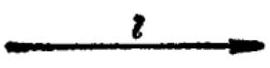
\includegraphics[max width=0.3\textwidth]{images/01912cc2-ffb6-728e-9ae7-b113ff05c64b_7_968321.jpg}
  	%\documentclass[tikz,border=5pt]{standalone}
\begin{document}
	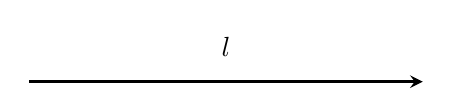
\begin{tikzpicture}
		% 绘制射线,从原点(0,0)出发向右延伸5cm,右侧有三角形箭头
		\draw[->, >=stealth, line width=1pt] (0,0) -- ++(5cm,0);
		% 在射线上方添加标签l
		\node[above] at (2.5cm, 0.2cm) {$l$};
	\end{tikzpicture}
\end{document}

  	\caption{图 1-1}
  \end{subfigure}
		\hfill % 两个图片之间添加空白填充,确保左右分布
% 右侧图片:宽度设置为0.45倍文本宽度
  \begin{subfigure}[h]{0.45\textwidth}
  \centering
%  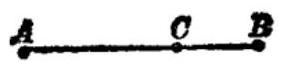
\includegraphics[max width=0.3\textwidth]{images/01912cc2-ffb6-728e-9ae7-b113ff05c64b_7_264987.jpg}
  %\documentclass[tikz,border=5pt]{standalone}
\begin{document}
	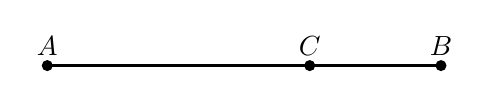
\begin{tikzpicture}
		% 绘制5cm长的线段AB
		\draw[line width=1pt] (0,0) -- (5cm,0);
		% 标记点A、B、C
		\fill (0,0) circle (2pt) node[above] {$A$};                % 点A(起点)
		\fill (5cm,0) circle (2pt) node[above] {$B$};              % 点B(终点)
		\fill (5cm - 5cm/3,0) circle (2pt) node[above] {$C$};      % 点C(距B点1/3处)
	\end{tikzpicture}
\end{document}

  \caption{图 1-2}
  \end{subfigure}
%  \caption{}
\end{figure}

一条线段也可以规定两个相反的方向. 如图 1-2 中的线段 \({AB}\) ,如果以 \(A\) 为起点、 \(B\) 为终点,那么,它的方向是从 \(A\) 到 \(B\) ; 相反,如果以 \(B\) 为起点、 \(A\) 为终点,它的方向就是从 \(B\) 到 \(A\) . 

\begin{definition}[有向线段] 
	规定了方向,即规定了起点和终点的线段叫做有向线段.
\end{definition}

 表示有向线段时, 要将表示起点的字母写在前面, 表示终点的字母写在后面. 如以 \(A\) 为起点、 \(B\) 为终点的有向线段记作 \(\overline{AB}\) . 图 1-2 中,点 \(C\) 是线段 \({AB}\) 上的一点, \(\overline{AB}\) 和 \(\overline{AC}\) 是方向相同的有向线段, \(\overline{AB}\) 和 \(\overline{BC}\) 是方向相反的有向线段.

\begin{definition}[线段的长度]
选定一条线段作为长度单位, 我们可以量得一条线段的长度,线段 \({AB}\) 的长度,就是有向线段 \(\overline{AB}\) 的长度,记作 \(\left| {AB}\right|\) .
\end{definition}

 如图 1-3,设线段 \(e\) 是长度单位,那么 \(\left| {AB}\right| = 3\) . 因为有向线段的长度与它的方向无关,所以 \(\left| {AB}\right| = \left| {BA}\right|\) .

\begin{figure}[h]
	\centering
	% 左侧图片:宽度设置为0.45倍文本宽度,预留间距
	\begin{subfigure}[h]{0.45\textwidth}
		\centering
%		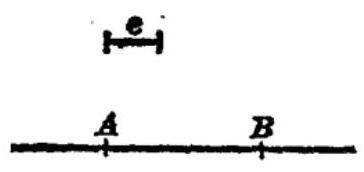
\includegraphics[max width=0.4\textwidth]{images/01912cc2-ffb6-728e-9ae7-b113ff05c64b_8_197225.jpg}
		%\documentclass[tikz, border=5pt]{standalone}
\begin{document}
	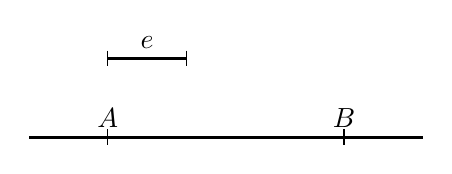
\begin{tikzpicture}
		% 绘制水平直线
		\draw[line width=1pt] (-2,0) -- (3,0);
		
		% 点A:标记文字、小竖线
		\node at (-1,0) [above] {$A$};
		\draw (-1,0.1) -- (-1,-0.1);  % A点的垂直小竖线(上下各延伸0.1单位)
		
		% 点B:标记文字、小竖线
		\node at (2,0) [above] {$B$};
		\draw (2,0.1) -- (2,-0.1);  % B点的垂直小竖线
		
		% 上方线段e:线段本身、两端小竖线、标记文字
		\draw[line width=1pt] (-1,1) -- (0,1);
		\draw (-1,1.1) -- (-1,0.9);  % e线段左端的垂直小竖线
		\draw (0,1.1) -- (0,0.9);  % e线段右端的垂直小竖线
		\node at (-0.5,1) [above] {$e$};
	\end{tikzpicture}
\end{document}

		\caption{图 1-3}
	\end{subfigure}
	\hfill % 两个图片之间添加空白填充,确保左右分布
	% 右侧图片:宽度设置为0.45倍文本宽度
	\begin{subfigure}[h]{0.45\textwidth}
		\centering
%		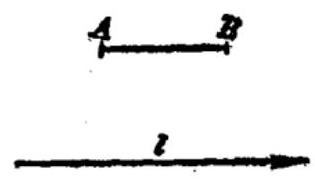
\includegraphics[max width=0.3\textwidth]{images/01912cc2-ffb6-728e-9ae7-b113ff05c64b_8_589831.jpg}
		%\documentclass[tikz, border=5pt]{standalone}
\begin{document}
	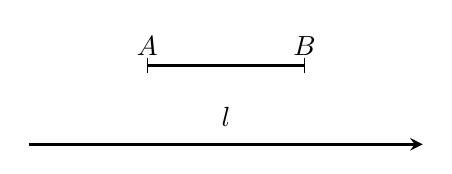
\begin{tikzpicture}

		% 绘制水平直线
		\draw[line width=1pt] (-1,1) -- (1,1);
		
		% 点A:标记文字、小竖线
		\node at (-1,1) [above] {$A$};
		\draw (-1,1.1) -- (-1,0.9);  % A点的垂直小竖线(上下各延伸0.1单位)
		
		% 点B:标记文字、小竖线
		\node at (1,1) [above] {$B$};
		\draw (1,1.1) -- (1,0.9);  % B点的垂直小竖线
		
		% 绘制射线,从原点(0,0)出发向右延伸5cm,右侧有三角形箭头
		\draw[->, >=stealth, line width=1pt] (-2.5,0) -- ++(5cm,0);
		% 在射线上方添加标签l
		\node[above] at (0cm, 0.1cm) {$l$};

	\end{tikzpicture}
\end{document}

		\caption{图 1-4}
	\end{subfigure}
	%  \caption{}
\end{figure}

如果有向线段在有向直线 \(l\) 上或与 \(l\) 平行,那么,它的方向与 \(l\) 的正方向可能相同或相反. 例如图 1-4 中的 \(\overline{AB}\) 与 \(l\) 的方向相同,而 \(\overline{BA}\) 与 \(l\) 的方向相反.

根据 \(\overline{AB}\) 与有向直线 \(l\) 的方向相同或相反,分别把它的长度加上正号或负号, 这样所得的数, 叫做有向线段的数量 (或数值). 有向线段 \(\overline{AB}\) 的数量用 \({AB}\) 表示*、显然

\[
    {AB} = - {BA}\text{. }
\]

\customfootnote{
	* 在引入有向直线以后,线段 \({AB}\) 的长度一律用 \(\left| {AB}\right|\) 表示.
}

数轴 \({Ox}\) 是有向直线,数轴上点 \(P\) 的坐标 \({x}_{0}\) 实际上是以有向线段的数量来定义的. 点 \(P\) 的坐标 \({x}_{0}\) 是以原点 \(O\) 为起点、 \(P\) 为终点的有向线段 \(\overline{OP}\) 的数量, \({OP} = {x}_{0}\) . 例如,点 \(A\text{、}B\) 的坐标分别是有向线段 \(\overline{OA}\text{、}\overline{OB}\) 的数量, \({OA} = 3\text{、}{OB} = - 2\) (图 1-5).

现在我们来研究, 对于数轴上任意一条有向线段, 怎样用它的起点坐标和终点坐标表示它的数量.

\begin{figure}[h]
  \centering
%  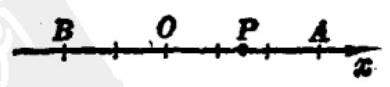
\includegraphics[max width=0.4\textwidth]{images/01912cc2-ffb6-728e-9ae7-b113ff05c64b_8_647013.jpg}
  %\documentclass[tikz, border=5pt]{standalone}
\begin{document}
	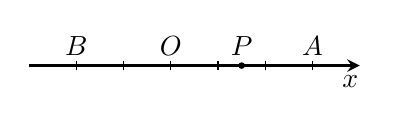
\begin{tikzpicture}[scale=0.6]
		% 绘制主水平线
		\draw[->, >=stealth, line width=1pt] (-1,0) -- (6,0);
		
		% 6个小竖线标记点(从左到右)
		\draw (0,0.1) -- (0,-0.1);    % 第一个竖线标记
		\draw (1,0.1) -- (1,-0.1);    % 第二个竖线标记
		\draw (2,0.1) -- (2,-0.1);    % 第三个竖线标记
		\draw (3,0.1) -- (3,-0.1);    % 第六个竖线标记
		\draw (4,0.1) -- (4,-0.1);    % 第四个竖线标记
		\draw (5,0.1) -- (5,-0.1);    % 第五个竖线标记

		% 实心圆点P
		\fill (3.5,0) circle (2pt) node[above] {$P$};  % 带标签的实心点
		
		% 为竖线标记添加标签
		\node[above] at (0,0) {$B$};
		\node[above] at (5,0) {$A$};
		\node[above] at (2,0) {$O$};
		\node[below] at (5.8,0) {$x$};
		
	\end{tikzpicture}
\end{document}


  \caption{图 1-5}
\end{figure}

设 \(\overline{AB}\) 是 \(x\) 轴上的任意一条有向线段, \(O\) 是原点. 先讨论两点 \(A\text{、}B\) 与 \(O\) 都不重合的情形. 如图 1-6,它们的位置关系只可能有六种不同情形. 点 \(A\text{、}B\) 的坐标分别用 \({x}_{1}\) 和 \({x}_{2}\) 表示,那么 \({OA} = {x}_{1},{OB} = {x}_{2}\) .

在图 1-6(1)中, \({AB} = \left| {AB}\right| ,{OA} = \left| {OA}\right| ,{OB} = \left| {OB}\right|\) ,而 \(\left| {AB}\right| = \left| {OB}\right| - \left| {OA}\right|\)

\[
  \therefore \;{AB} = {OB} - {OA}\text{,}
\]

即

\[
    {AB} = {x}_{2} - {x}_{1}\text{. }
\]

\begin{figure}[h]
  \centering
%  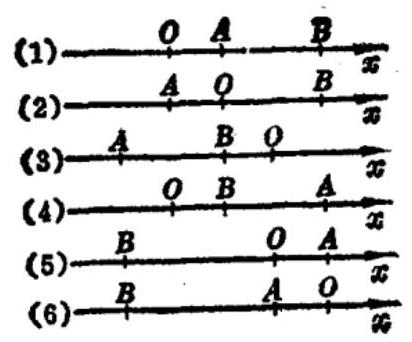
\includegraphics[max width=0.4\textwidth]{images/01912cc2-ffb6-728e-9ae7-b113ff05c64b_9_561693.jpg}
  %\documentclass[tikz, border=5pt]{standalone}
\begin{document}
	% 图(1)
	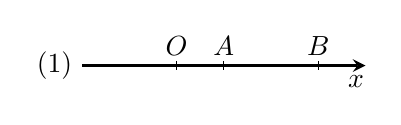
\begin{tikzpicture}[scale=0.6]
		\node[left] at (-1, 0) {(1)};            % 左编号
		% 绘制主水平线
		\draw[->, >=stealth, line width=1pt] (-1,0) -- (5,0);
		\node[below] at (4.8,0) {$x$};
	
		% 6个小竖线标记点(从左到右)
		\draw (1,0.1) -- (1,-0.1); \node[above] at (1,0) {$O$};   % 第一个竖线标记
		\draw (2,0.1) -- (2,-0.1); \node[above] at (2,0) {$A$};   % 第二个竖线标记
		\draw (4,0.1) -- (4,-0.1); \node[above] at (4,0) {$B$};   % 第三个竖线标记
	\end{tikzpicture}
	
	% 图(2)
	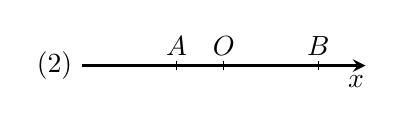
\begin{tikzpicture}[scale=0.6]
		\node[left] at (-1, 0) {(2)}; 		% 左编号
		\draw[->, >=stealth, line width=1pt] (-1,0) -- (5,0); 		% 绘制水平线
		\node[below] at (4.8,0) {$x$}; 
		\foreach \pos/\label in {1/A, 2/O, 4/B} {    % 点O、A、B的位置
			\draw (\pos, 0.1) -- (\pos, -0.1);       % 竖线标记
			\node[above] at (\pos, 0) {$\label$};    % 点标签(上方)
		}
	\end{tikzpicture}
	
	% 图(3)
	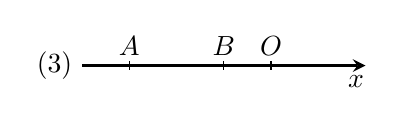
\begin{tikzpicture}[scale=0.6]
		\node[left] at (-1, 0) {(3)}; 		% 左编号
		\draw[->, >=stealth, line width=1pt] (-1,0) -- (5,0); 		% 绘制水平线
		\node[below] at (4.8,0) {$x$}; 
		\foreach \pos/\label in {0/A, 2/B, 3/O} {
			\draw (\pos, 0.1) -- (\pos, -0.1);
			\node[above] at (\pos, 0) {$\label$};
		}
	\end{tikzpicture}
	
	% 图(4)
	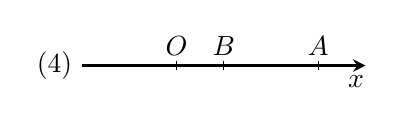
\begin{tikzpicture}[scale=0.6]
		\node[left] at (-1, 0) {(4)}; 		% 左编号
		\draw[->, >=stealth, line width=1pt] (-1,0) -- (5,0); 		% 绘制水平线
		\node[below] at (4.8,0) {$x$}; 
		\foreach \pos/\label in {1/O, 2/B, 4/A} {
			\draw (\pos, 0.1) -- (\pos, -0.1);
			\node[above] at (\pos, 0) {$\label$};
		}
	\end{tikzpicture}
	
	% 图(5)
	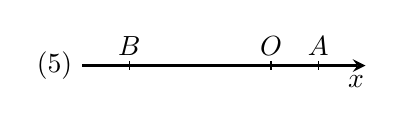
\begin{tikzpicture}[scale=0.6]
		\node[left] at (-1, 0) {(5)}; 		% 左编号
		\draw[->, >=stealth, line width=1pt] (-1,0) -- (5,0); 		% 绘制水平线
		\node[below] at (4.8,0) {$x$}; 
		\foreach \pos/\label in {0/B, 3/O, 4/A} {
			\draw (\pos, 0.1) -- (\pos, -0.1);
			\node[above] at (\pos, 0) {$\label$};
		}
	\end{tikzpicture}
	
	% 图(6)
	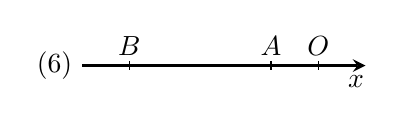
\begin{tikzpicture}[scale=0.6]
		\node[left] at (-1, 0) {(6)}; 		% 左编号
		\draw[->, >=stealth, line width=1pt] (-1,0) -- (5,0); 		% 绘制水平线
		\node[below] at (4.8,0) {$x$}; 
		\foreach \pos/\label in {0/B, 3/A, 4/O} {
			\draw (\pos, 0.1) -- (\pos, -0.1);
			\node[above] at (\pos, 0) {$\label$};
		}
	\end{tikzpicture}
	
\end{document}

  \caption{图 1-6}
\end{figure}

在图 1-6(2)中, \({AB} = \left| {AB}\right| ,{OA} = - \left| {OA}\right| ,{OB} = \left| {OB}\right|\) ,而 \(\left| {AB}\right| = \left| {OA}\right| + \left| {OB}\right|\) ,

\[
  \therefore \;{AB} = {OB} - {OA}\text{,}
\]

即

\[
    {AB} = {x}_{2} - {x}_{1}
\]

同样可以证明, 对于其他四种情况, 这个等式也成立. 容易验证,当点 \(A\) 或点 \(B\) 与原点 \(O\) 重合时这个等式同样成立. 因此,对于数轴上任意有向线段 \(\overline{AB}\) ,它的数量 \({AB}\) 和起点坐标 \({x}_{1}\) 、终点坐标 \({x}_{2}\) 有如下关系:

\[
    {AB} = {x}_{2} - {x}_{1}
\]
\begin{corollary}[数轴两点的距离公式]
根据这个公式可以得到,数轴上两点 \(A\text{、}B\) 的距离公式
\[
  \left| {AB}\right| = \left| {{x}_{2} - {x}_{1}}\right| \text{. }
\]
\end{corollary}
下面, 我们来求平面上任意两点的距离.

在直角坐标系中,已知两点 \({P}_{1}\left( {{x}_{1},{y}_{1}}\right) \text{、}{P}_{2}\left( {{x}_{2},{y}_{2}}\right)\) (图 1-7). 从 \({P}_{1}\text{、}{P}_{2}\) 分别向 \(x\) 轴和 \(y\) 轴作垂线 \({P}_{1}{M}_{1}\text{、}{P}_{1}{N}_{1}\) 和 \({P}_{2}{M}_{2}\text{、}{P}_{2}{N}_{2}\) ,垂足分别为 \({M}_{1}\left( {{x}_{1},0}\right)\) 、 \({N}_{1}\left( {0,{y}_{1}}\right) \text{、}{M}_{2}\left( {{x}_{2},0}\right) \text{、}{N}_{2}\left( {0,{y}_{2}}\right)\) ,其中直线 \({P}_{1}{N}_{1}\) 和 \({P}_{2}{M}_{2}\) 相交于点 \(Q\) .

\begin{figure}[h]
  \centering
%  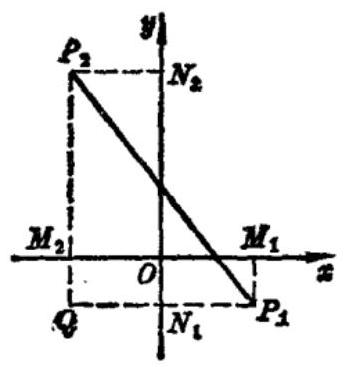
\includegraphics[max width=0.4\textwidth]{images/01912cc2-ffb6-728e-9ae7-b113ff05c64b_10_261177.jpg}
  %\documentclass[tikz, border=5pt]{standalone}
\begin{document}
	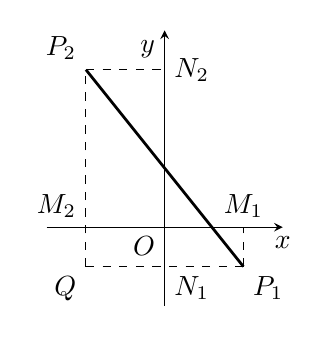
\begin{tikzpicture}[>=stealth, scale=0.5] % 箭头样式为stealth,
		
		% 绘制坐标轴
		\draw[->] (-3,0) -- (3,0) node[below] {$x$}; % x轴(带箭头和标签)
		\draw[->] (0,-2) -- (0,5) node[below left] {$y$}; % y轴(带箭头和标签)
		\node at (0,0) [below left] {$O$};           % 原点O的标签
		
		% 定义各关键点坐标
		\coordinate (P1) at (2,-1);  % 点P₁
		\coordinate (P2) at (-2,4); % 点P₂
		\coordinate (N1) at (0,-1); % 点N₁
		\coordinate (N2) at (0,4);  % 点N₂
		\coordinate (M1) at (2,0);  % 点M₁
		\coordinate (M2) at (-2,0); % 点M₂
		\coordinate (Q)  at (-2,-1);% 点Q
		
		% 绘制连接P₁和P₂的直线
		\draw[line width=1pt] (P1) -- (P2);
		
		% 绘制虚线辅助线(矩形的边)
		\draw[dashed] (P2) -- (N2); % P₂到y轴的虚线
		\draw[dashed] (Q) -- (P2);  % Q到P₂的虚线
		\draw[dashed] (Q) -- (P1);  % Q到P₁的虚线
		\draw[dashed] (P1) -- (M1); % P₁到x轴的虚线
		
		% 标记各点的标签
		\node at (P1) [below right]  {$P_1$};
		\node at (P2) [above left]      {$P_2$};
		\node at (N1) [below right] {$N_1$};
		\node at (N2) [right]             {$N_2$};
		\node at (M1) [above]          {$M_1$};
		\node at (M2) [above left] {$M_2$};
		\node at (Q)  [below left]   {$Q$};
		
	\end{tikzpicture}
\end{document}

  \caption{图 1-7}
\end{figure}

在 \({Rt}\bigtriangleup {P}_{1}Q{P}_{2}\) 中,
\[
{\left| {P}_{1}{P}_{2}\right| }^{2} = {\left| {P}_{1}Q\right| }^{2} + {\left| Q{P}_{2}\right| }^{2} .
\]
\[
\because \;\left| {{P}_{1}Q}\right| = \left| {{M}_{1}{M}_{2}}\right| = \left| {{x}_{2} - {x}_{1}}\right| , 
\]
\[
\left| {Q{P}_{2}}\right| = \left| {{N}_{1}{N}_{2}}\right| = \left| {{y}_{2} - {y}_{1}}\right| ,
\]
\[
  \therefore {\left| {P}_{1}{P}_{2}\right| }^{2} = {\left| {x}_{2} - {x}_{1}\right| }^{2} + {\left| {y}_{2} - {y}_{1}\right| }^{2}\text{.}
\]
\begin{corollary}[两点间距离公式]
由此得到两点 \({P}_{1}\left( {{x}_{1},{y}_{1}}\right) \text{、}{P}_{2}\left( {{x}_{2},{y}_{2}}\right)\) 的距离公式:
\[
  \left| {{\mathbf{P}}_{1}{\mathbf{P}}_{2}}\right| = \sqrt{{\left( {x}_{2} - {x}_{1}\right) }^{2} + {\left( {y}_{2} - {y}_{1}\right) }^{2}}.
\]
\end{corollary}
例 1 已知数轴上三点 \(A\text{、}B\text{、}C\) 的坐标分别是 4、 -2 、 -6. 求 \(\overline{AB}\text{、}\overline{BC}\text{、}\overline{CA}\) 的数量和长度 (图 1-8).

\begin{figure}[h]
  \centering
%  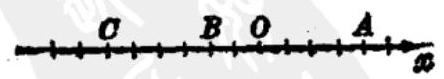
\includegraphics[max width=0.5\textwidth]{images/01912cc2-ffb6-728e-9ae7-b113ff05c64b_10_794091.jpg}
  %\documentclass[tikz, border=5pt]{standalone}
\begin{document}
	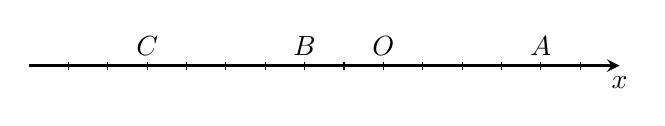
\begin{tikzpicture}[scale=0.5]
		% 绘制带箭头的 x 轴
		\draw[->, >=stealth, line width=1pt] (-9,0) -- (6,0) node[below] {$x$};
		
		% 定义各点坐标(可根据刻度密度调整)
		\coordinate (C) at (-6,0);  % 点 C
		\coordinate (B) at (-2,0);  % 点 B
		\coordinate (O) at (0,0);   % 原点 O
		\coordinate (A) at (4,0);   % 点 A
		
		% 绘制所有小刻度线(从 -8 到 5,每隔 1 单位画竖线)
		\foreach \x in {-8,-7,...,5} {
			\draw (\x, 0.1) -- (\x, -0.1);  % 小竖线(长 0.2 单位)
		}
		
		% 标记各点标签(位置与原图匹配)
		\node[above] at (C) {$C$};
		\node[above] at (B) {$B$};
		\node[above] at (O) {$O$};
		\node[above] at (A) {$A$};
	\end{tikzpicture}
\end{document}

  \caption{图 1-8}
\end{figure}

解: \({AB} = \left( {-2}\right) - 4 = - 6,\;\left| {AB}\right| = \left| {-6}\right| = 6\) ;

\[
    {BC} = - 6 - \left( {-2}\right) = - 4,\left| {BC}\right| = \left| {-4}\right| = 4\text{;}
\]

\[
    {CA} = 4 - \left( {-6}\right) = {10},\;\left| {CA}\right| = \left| {10}\right| = {10}.
\]

例 2 \(\bigtriangleup {ABC}\) 中, \({AO}\) 是 \({BC}\) 边上的中线 (图 1-9). 求证:

\[
    {\left| AB\right| }^{2} + {\left| AC\right| }^{2} = 2\left( {{\left| AO\right| }^{2} + {\left| OC\right| }^{2}}\right) .
\]

\begin{figure}[h]
  \centering
%  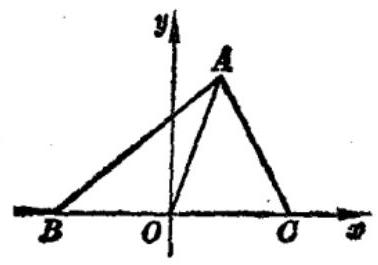
\includegraphics[max width=0.4\textwidth]{images/01912cc2-ffb6-728e-9ae7-b113ff05c64b_11_761140.jpg}
  %\documentclass[tikz, border=5pt]{standalone}
\begin{document}
	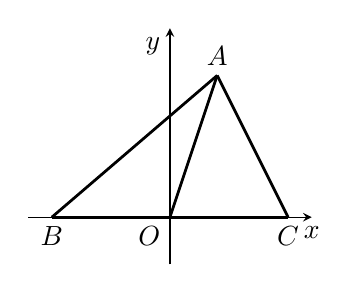
\begin{tikzpicture}[>=stealth, scale=0.6] % 箭头样式为stealth,
		
		% 绘制坐标轴
		\draw[->] (-3,0) -- (3,0) node[below] {$x$};      % x轴(带箭头和标签)
		\draw[->] (0,-1) -- (0,4) node[below left] {$y$}; % y轴(带箭头和标签)
		\node at (0,0) [below left] {$O$};                % 原点O的标签
		
		% 定义各关键点坐标
		\coordinate (A) at (1,3);    % 点A
		\coordinate (B) at (-2.5,0); % 点B
		\coordinate (C) at (2.5,0);  % 点C
		\coordinate (O) at (0,0);   % 原点 O
		
		% 绘制连接点的直线
		\draw[line width=1pt] (A) -- (B);
		\draw[line width=1pt] (A) -- (C);
		\draw[line width=1pt] (A) -- (O);
		\draw[line width=1pt] (B) -- (C);
		
		% 标记各点的标签
		\node at (B) [below] {$B$};
		\node at (A) [above] {$A$};
		\node at (C) [below] {$C$};
		
	\end{tikzpicture}
\end{document}

  \caption{图 1-9}
\end{figure}

证明: 取线段 \({BC}\) 所在的直线为 \(x\) 轴,点 \(O\) 为原点建立直角坐标系. 设点 \(A\) 的坐标为 \(\left( {b,c}\right)\) ,点 \(C\) 的坐标为 \(\left( {a,0}\right)\) , 则点 \(B\) 的坐标为 \(\left( {-a,0}\right)\) . 可得

\[
    {\left| AB\right| }^{2} = {\left( a + b\right) }^{2} + {c}^{2},{\left| AC\right| }^{2} = {\left( a - b\right) }^{2} + {c}^{2},
\]

\[
    {\left| AO\right| }^{2} = {b}^{2} + {c}^{2},\;{\left| OC\right| }^{2} = {a}^{2}.
\]

\[
  \therefore {\left| AB\right| }^{2} + {\left| AC\right| }^{2} = 2\left( {{a}^{2} + {b}^{2} + {c}^{2}}\right) ,
\]

\[
    {\left| AO\right| }^{2} + {\left| OC\right| }^{2} = {a}^{2} + {b}^{2} + {c}^{2}.
\]

\(\therefore {\left| AB\right| }^{2} + {\left| AC\right| }^{2} = 2\left( {{\left| AO\right| }^{2} + {\left| OC\right| }^{2}}\right)\) .

\begin{problemset}[练习]

\item 数轴上点 \(A\) 的坐标为 2,点 \(B\) 的坐标为 -3 . 验证公式 \({AB} = {x}_{2} - {x}_{1}.\)

\item 已知数轴 \(x\) 上的点 \(A\text{、}B\text{、}C\) 的坐标分别为 \(1\text{、}2\text{、}3\) . (1) 求 \(\overline{AB}\text{、}\overline{CB}\) 的数量; (2) 如果在 \(x\) 轴上还有两个点 \(D\text{、}E\) ,且 \({AD} = {2.5},{CE} = - 3\) . 求点 \(D\text{、}E\) 的坐标.

\item 求有下列坐标的两点距离:

(1) \(\left( {6,0}\right) \text{、}\left( {-2,0}\right)\) ; (2) \(\left( {0, - 4}\right) \text{、}\left( {0, - 1}\right)\) ;

(3) \(\left( {6,0}\right) \text{、}\left( {0, - 2}\right)\) ; (4) \(\left( {2,1}\right) \text{、}\left( {5, - 1}\right)\) ;

(5) \(\left( {\frac{\sqrt{3}}{2}, - \frac{\sqrt{2}}{2}}\right) ,\left( {-\frac{\sqrt{2}}{2}, - \frac{\sqrt{3}}{2}}\right)\) ;

(6) \(\left( {a{b}^{2},{2abc}}\right) \text{、}\left( {a{c}^{2},0}\right)\) .

\item 已知点 \(A\left( {a, - 5}\right)\) 和 \(B\left( {0,{10}}\right)\) 的距离是 17,求 \(a\) 的值.

\end{problemset}

\section{线段的定比分点}

\begin{definition}[定比分点] \label{def:int}
	
有向直线 \(l\) 上的一点 \(P\) ,把 \(l\) 上的有向线段 \(\overline{{P}_{1}{P}_{2}}\) 分成两条有向线段 \(\overline{{P}_{1}P}\) 和 \(\overline{P{P}_{2}}.\overline{{P}_{1}P}\) 和 \(\overline{P{P}_{2}}\) 数量的比叫做点 \(P\) 分 \(\overline{{\mathbf{P}}_{1}{\mathbf{P}}_{2}}\) 所成的比,通常用字母 \(\lambda\) 来表示这个比值,

\[
  \lambda = \frac{{P}_{1}P}{P{P}_{2}}
\]

点 \(P\) 叫做 \(\overline{{P}_{1}{P}_{2}}\) 的定比分点.
\end{definition}

\begin{corollary}[内外分点]
如果点 \(P\) 在线段 \({P}_{1}{P}_{2}\) 上 (图 1-10 甲),点 \(P\) 叫做 \(\overline{{P}_{1}{P}_{2}}\) 的内分点. 这时,无论 \(l\) 的方向如何, \(\overline{{P}_{1}P}\) 和 \(\overline{P{P}_{2}}\) 的方向都相同,它们的数量的符号也相同,所以 \(\lambda\) 为正值. 如果点 \(P\) 在线段 \({P}_{2}{P}_{1}\) 或 \({P}_{1}{P}_{2}\) 的延长线上 (图 1-10乙、丙),点 \(P\) 叫做 \(\overline{{P}_{1}{P}_{2}}\) 的外分点. 这时无论 \(l\) 的方向如何, \(\overline{{P}_{1}P}\) 和 \(\overline{P{P}_{2}}\) 的方向都相反, 它们的数量的符号也相反,所以 \(\lambda\) 为负值.
\end{corollary}

\begin{figure}[h]
  \centering
%  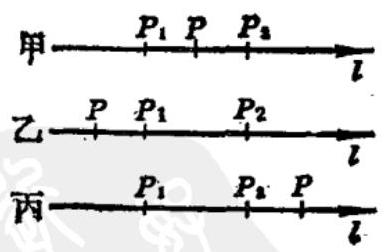
\includegraphics[max width=0.4\textwidth]{images/01912cc2-ffb6-728e-9ae7-b113ff05c64b_12_791347.jpg}
  %\documentclass[ctex,tikz, border=5pt]{standalone}
\begin{document}
	% 图(1)
	\begin{tikzpicture}[scale=0.6]
		\node[left] at (-1, 0) {(甲)};            % 左编号
		% 绘制主水平线
		\draw[->, >=stealth, line width=1pt] (-1,0) -- (5,0);
		\node[below] at (4.8,0) {$l$};
		
		% 6个小竖线标记点(从左到右)
		\draw (1,0.1) -- (1,-0.1); \node[above] at (1,0) {$P_1$};   % 第一个竖线标记
		\draw (2,0.1) -- (2,-0.1); \node[above] at (2,0) {$P$};   % 第二个竖线标记
		\draw (3,0.1) -- (3,-0.1); \node[above] at (3,0) {$P_2$};   % 第三个竖线标记
	\end{tikzpicture}
	
	% 图(2)
	\begin{tikzpicture}[scale=0.6]
		\node[left] at (-1, 0) {(乙)}; 		% 左编号
		\draw[->, >=stealth, line width=1pt] (-1,0) -- (5,0); 		% 绘制水平线
		\node[below] at (4.8,0) {$l$}; 
		\foreach \pos/\label in {0/P, 1/P_1, 3/P_2} {    % 点P、P₂、P₁的位置
			\draw (\pos, 0.1) -- (\pos, -0.1);       % 竖线标记
			\node[above] at (\pos, 0) {$\label$};    % 点标签(上方)
		}
	\end{tikzpicture}
	
	% 图(3)
	\begin{tikzpicture}[scale=0.6]
		\node[left] at (-1, 0) {(丙)}; 		% 左编号
		\draw[->, >=stealth, line width=1pt] (-1,0) -- (5,0); 		% 绘制水平线
		\node[below] at (4.8,0) {$l$}; 
		\foreach \pos/\label in {1/P_1, 3/P_2, 4/P} {
			\draw (\pos, 0.1) -- (\pos, -0.1);
			\node[above] at (\pos, 0) {$\label$};
		}
	\end{tikzpicture}
	
\end{document}

  \caption{图 1-10}
\end{figure}

由于点 \(P\) 分 \(\overline{{P}_{1}{P}_{2}}\) 所成的比与它们所在的直线 \(l\) 的方向无关,为了简便起见,在以后谈到点 \(P\) 分 \(\overline{{P}_{1}{P}_{2}}\) 所成的比时,一般不提它所在的有向直线的方向.

设 \(\overline{{P}_{1}{P}_{2}}\) 的两个端点分别为 \({P}_{1}\left( {{x}_{1},{y}_{1}}\right)\) 和 \({P}_{2}\left( {{x}_{2},{y}_{2}}\right)\) ,点 \(P\) 分 \(\overline{{P}_{1}{P}_{2}}\) 所成的比为 \(\lambda \;\left( {\lambda \neq - 1}\right)\) (图 1-11),求分点 \(P\) 的坐标 \(\left( {x,y}\right)\) .

\begin{figure}[h]
	\centering
	%  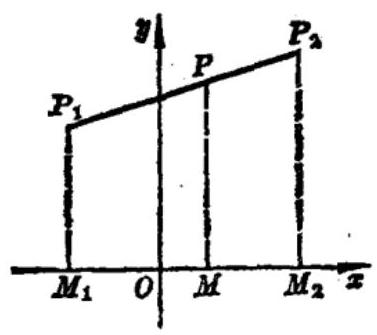
\includegraphics[max width=0.4\textwidth]{images/01912cc2-ffb6-728e-9ae7-b113ff05c64b_13_700827.jpg}
	%\documentclass[tikz, border=5pt]{standalone}
\begin{document}
	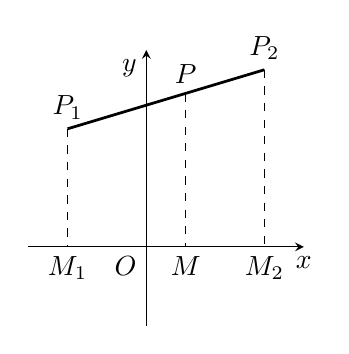
\begin{tikzpicture}[>=stealth, scale=0.5] % 箭头样式为stealth,
		
		% 绘制坐标轴
		\draw[->] (-3,0) -- (4,0) node[below] {$x$};      % x轴(带箭头和标签)
		\draw[->] (0,-2) -- (0,5) node[below left] {$y$}; % y轴(带箭头和标签)
		\node at (0,0) [below left] {$O$};                % 原点O的标签
		
		% 定义各关键点坐标
		\coordinate (P1) at (-2,3); % 点P₁
		\coordinate (P2) at (3,4.5);  % 点P₂
		\coordinate (P) at (1,3.9);  % 点P
		\coordinate (M1) at (-2,0); % 点M₁
		\coordinate (M2) at (3,0);  % 点M₂
		\coordinate (M) at (1,0);   % 点M
		
		% 绘制连接P₁和P₂的直线
		\draw[line width=1pt] (P1) -- (P2);
		
		% 绘制虚线辅助线(矩形的边)
		\draw[dashed] (P1) -- (M1); % P₁到x轴的虚线
		\draw[dashed] (P2) -- (M2); % P₂到x轴的虚线
		\draw[dashed] (P) -- (M);  % M到P的虚线
		
		% 标记各点的标签
		\node at (P1) [above] {$P_1$};
		\node at (P2) [above]  {$P_2$};
		\node at (P) [above]  {$P$};
		\node at (M1) [below]  {$M_1$};
		\node at (M2) [below]  {$M_2$};
		\node at (M) [below]  {$M$};
		
	\end{tikzpicture}
\end{document}

	\caption{图 1-11}
\end{figure}

过点 \({P}_{1}\text{、}{P}_{2}\text{、}P\) 分别作 \(x\) 轴的垂线 \({P}_{1}{M}_{1}\text{、}{P}_{2}{M}_{2}\text{、}{PM}\) ,则垂足分别为 \({M}_{1}\left( {{x}_{1},0}\right) \text{、}{M}_{2}\left( {{x}_{2},0}\right) \text{、}M\left( {x,0}\right)\) . 根据平行线分线段成比例定理, 得

\[
  \frac{\left| {P}_{1}P\right| }{\left| P{P}_{2}\right| } = \frac{\left| {M}_{1}M\right| }{\left| M{M}_{2}\right| }.
\]

如果点 \(P\) 在线段 \({P}_{1}{P}_{2}\) 上,那么点 \(M\) 也在线段 \({M}_{1}{M}_{2}\) 上; 如果点 \(P\) 在线段 \({P}_{1}{P}_{2}\) 或 \({P}_{2}{P}_{1}\) 的延长线上,那么点 \(M\) 也在线段 \({M}_{1}{M}_{2}\) 或 \({M}_{2}{M}_{1}\) 的延长线上. 因此 \(\frac{{P}_{1}P}{P{P}_{2}}\) 与 \(\frac{{M}_{1}M}{M{M}_{2}}\) 的符号相同, 所以

\[
  \frac{{P}_{1}P}{P{P}_{2}} = \frac{{M}_{1}M}{M{M}_{2}}.
\]

\[
  \because \;{M}_{1}M = x - {x}_{1},
\]

\[
  M{M}_{2} = {x}_{2} - x,
\]

\[
  \therefore \lambda = \frac{x - {x}_{1}}{{x}_{2} - x}
\]

即 \(\left( {1 + \lambda }\right) x = {x}_{1} + \lambda {x}_{2}\) ,当 \(\lambda \neq - 1\) 时,

得

\[
  x = \frac{{x}_{1} + \lambda {x}_{2}}{1 + \lambda }
\]

同理可以求得 \(\lambda = \frac{y - {y}_{1}}{{y}_{2} - y}\) ,

\[
  y = \frac{{y}_{1} + \lambda {y}_{2}}{1 + \lambda }
\]

\begin{corollary}[定比分点的坐标]

因此,当已知两个端点为 \({P}_{1}\left( {{x}_{1},{y}_{1}}\right) \text{、}{P}_{2}\left( {{x}_{2},{y}_{2}}\right)\) ,点 \(P\left( {x,y}\right)\) 分 \(\overline{{P}_{1}{P}_{2}}\) 所成的比为 \(\lambda\) 时,点 \(P\) 的坐标是
\[
  x = \frac{{x}_{1} + \lambda {x}_{2}}{1 + \lambda },y = \frac{{y}_{1} + \lambda {y}_{2}}{1 + \lambda }\left( {\lambda \neq - 1}\right) .
\]
\end{corollary}

\begin{corollary}[中点的坐标]

当点 \(P\) 是线段 \(\overline{{P}_{1}{P}_{2}}\) 的中点时,有 \({P}_{1}P = P{P}_{2}\) ,即 \(\lambda = 1\) . 因此线段 \(\overline{{P}_{1}{P}_{2}}\) 中点 \(P\) 的坐标是
\[
\mathbf{x} = \frac{{\mathbf{x}}_{1} + {\mathbf{x}}_{2}}{2},\;\mathbf{y} = \frac{{\mathbf{y}}_{1} + {\mathbf{y}}_{2}}{2}.
\]
\end{corollary}


例 1 点 \({P}_{1}\) 和 \({P}_{2}\) 的坐标分别是 \(\left( {-1, - 6}\right)\) 和 \(\left( {3,0}\right)\) ,点 \(P\) 的横坐标为 \(- \frac{7}{3}\) . 求点 \(P\) 分 \(\overline{{P}_{1}{P}_{2}}\) 所成的比 \(\lambda\) 和点 \(P\) 的纵坐标 \(y\) .

\begin{figure}[h]
	\centering
	%  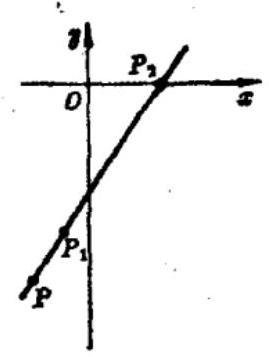
\includegraphics[max width=0.3\textwidth]{images/01912cc2-ffb6-728e-9ae7-b113ff05c64b_14_690449.jpg}
	%\documentclass[tikz, border=5pt]{standalone}
\begin{document}
	\begin{tikzpicture}[>=stealth, scale=0.5] % 箭头样式为 stealth,整体缩放优化显示
		
		% 绘制坐标轴
		\draw[->] (-3,0) -- (4.5,0) node[below] {$x$}; % x 轴(带箭头与标签)
		\draw[->] (0,-9) -- (0,1.5) node[below left] {$y$}; % y 轴(带箭头与标签)
		\node at (0,0) [below left] {$O$}; % 原点 $O$ 的标签
		
		% 定义各关键点坐标(可根据图形比例调整)
		\coordinate (P1) at (-1,-6);   % 点 $P_1$
		\coordinate (P2)  at (3,0);    % 点 $P$
		\coordinate (P) at (-7/3,-8);    % 点 $P_2$
		
		% 绘制连接 $P_1, P, P_2$ 的直线
		\draw [line width=1pt] (-8/3,-8.5) -- (10/3,0.5)  ;
		
		% 标记各点的标签 实心圆点
		\fill (P) circle (2pt) node [right] {$P$};  % 带标签的实心点
		\fill (P1) circle (2pt) node [left]  {$P_1$};  % 带标签的实心点
		\fill (P2) circle (2pt) node [above left]  {$P_2$};  % 带标签的实心点

	\end{tikzpicture}
\end{document}

	\caption{图 1-12}
\end{figure}

解: 由 \(\lambda\) 的定义,可得

\[
  \lambda = \frac{x - {x}_{1}}{{x}_{2} - x} = \frac{-\frac{7}{3} - \left( {-1}\right) }{3 - \left( {-\frac{7}{3}}\right) } = - \frac{1}{4}.
\]

\[
  y = \frac{{y}_{1} + \lambda {y}_{2}}{1 + \lambda } = \frac{-6 + \left( {-\frac{1}{4}}\right) \cdot 0}{1 + \left( {-\frac{1}{4}}\right) } = - 8.
\]

点 \(P\) 分 \({\overline{{P}_{1}P}}_{2}\) 所成的比是 \(- \frac{1}{4}\) ,点 \(P\) 的纵坐标是 \(- 8\) (图 1-12).

例 2 已知三角形顶点是 \(A\left( {{x}_{1},{y}_{1}}\right) \text{、}B\left( {{x}_{2},{y}_{2}}\right) \text{、}C\left( {{x}_{3},{y}_{3}}\right)\) . 求 \(\bigtriangleup {ABC}\) 的重心 \(G\) 的坐标 \(\left( {x,y}\right)\) (图 1-13).

\begin{figure}[h]
	\centering
	%  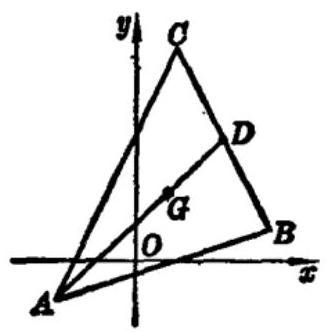
\includegraphics[max width=0.3\textwidth]{images/01912cc2-ffb6-728e-9ae7-b113ff05c64b_15_210180.jpg}
	%\documentclass[tikz,border=5pt]{standalone}
\begin{document}
	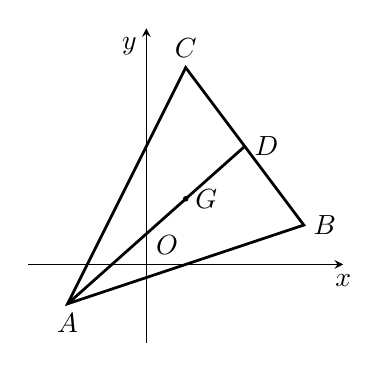
\begin{tikzpicture}[>=stealth, scale=0.5]
		% 绘制坐标轴
\draw[->] (-3,0) -- (5,0) node[below] {$x$}; % x 轴(带箭头与标签)
\draw[->] (0,-2) -- (0,6) node[below left] {$y$}; % y 轴(带箭头与标签)
\node at (0,0) [above right] {$O$}; % 原点 $O$ 的标签

% 定义各关键点坐标(可根据图形比例调整)
\coordinate (A) at (-2,-1);   % 点 $A$
\coordinate (B)  at (4,1);    % 点 $B$
\coordinate (C) at (1,5);    % 点 $C$
\coordinate (G) at (1,5/3);    % 点 $G$ 计算重心G的坐标 (重心坐标 = 三个顶点坐标的平均值)
\coordinate (D) at (2.5,3);    % 点 $D$

% 绘制连线
\draw [line width=1pt] (A) -- (B) -- (C) -- cycle; % 绘制三角形
\draw [line width=1pt] (A) -- (D);  % 绘制三条中线(从顶点到对边中点)

% 标记各点的标签 实心圆点
\fill (G) circle (2pt) node [right] {$G$};  % 带标签的实心点
\node at (A) [below] {$A$}; 
\node at (B) [right] {$B$}; 
\node at (C) [above] {$C$}; 
\node at (D) [right] {$D$}; 

	\end{tikzpicture}
\end{document}

	\caption{图 1-13}
\end{figure}

解: 设 \({BC}\) 边的中点为 \(D\) ,则点 \(D\) 的坐标是

\[
  \left( {\frac{{x}_{2} + {x}_{3}}{2},\frac{{y}_{2} + {y}_{3}}{2}}\right)
\]

又因为 \({AD}\) 是中线,且 \(\frac{AG}{GD} = 2\) ,所以点 \(G\) 的坐标是

\[
  x = \frac{{x}_{1} + 2 \times \frac{{x}_{2} + {x}_{3}}{2}}{1 + 2}
\]

\[
  y = \frac{{y}_{1} + 2 \times \frac{{y}_{2} + {y}_{3}}{2}}{1 + 2}
\]

整理后得重心 \(G\) 的坐标

\[
  x = \frac{{x}_{1} + {x}_{2} + {x}_{3}}{3},\;y = \frac{{y}_{1} + {y}_{2} + {y}_{3}}{3}.
\]

\begin{problemset}[练习]

\item 已知两点 \({P}_{1}\left( {3, - 2}\right) \text{、}{P}_{2}\left( {-9,4}\right)\) . 求点 \(P\left( {x,0}\right)\) 分 \(\overline{{P}_{1}{P}_{2}}\) 所成的比 \(\lambda\) 及 \(x\) 的值.

\item 点 \(M\) 分有向线段 \(\overline{{M}_{1}{M}_{2}}\) 的比为 \(\lambda\) ,求点 \(M\) 的坐标 \(\left( {x,y}\right)\) :

(1) 已知: \({M}_{1}\left( {1,5}\right) \text{、}{M}_{2}\left( {2,3}\right) ,\lambda = \frac{1}{3}\) ;

(2)已知: \({M}_{1}\left( {1,5}\right) \text{、}{M}_{2}\left( {2,3}\right) ,\lambda = - 2\) ;

(3) 已知: \({M}_{1}\left( {1,5}\right) \text{、}{M}_{2}\left( {2, - 3}\right) ,\lambda = - 2\) .

\item 已知 \(\bigtriangleup {ABC}\) 的顶点 \(A\left( {2,3}\right) \text{、}B\left( {8, - 4}\right)\) 和重心 \(G\left( {2, - 1}\right)\) . 求点 \(C\) 的坐标 \(\left( {x,y}\right)\) .

\end{problemset}

\begin{problemset}[习 题 一]

\item 如图, 数轴上每一格等于一个长度单位,说出有向线段 \(\overline{AB}\) 、\(\overline{BC}\text{、}\overline{CD}\) 和 \(\overline{EA}\) 的长度和数量. (第 1 题)
\begin{figure}[h]
  \centering
%  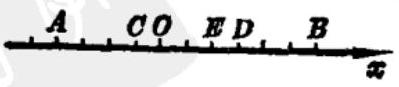
\includegraphics[max width=0.4\textwidth]{images/01912cc2-ffb6-728e-9ae7-b113ff05c64b_15_328018.jpg}
  %\documentclass[tikz, border=5pt]{standalone}
\begin{document}
	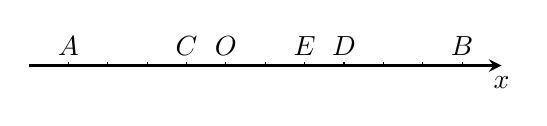
\begin{tikzpicture}[scale=0.5]
		% 绘制带箭头的 x 轴
		\draw[->, >=stealth, line width=1pt] (-5,0) -- (7,0) node[below] {$x$};
		
		% 定义各点坐标(可根据刻度密度调整)
		\coordinate (C) at (-1,0);  % 点 C
		\coordinate (B) at (6,0);  % 点 B
		\coordinate (O) at (0,0);   % 原点 O
		\coordinate (A) at (-4,0);   % 点 A
		\coordinate (D) at (3,0);  % 点 D
		\coordinate (E) at (2,0);  % 点 E

		% 绘制所有小刻度线(从 -5 到 6,每隔 1 单位画竖线)
		\foreach \x in {-4,-3,...,6} {
			\draw (\x, 0.1) -- (\x, 0);  % 小竖线(长 0.1 单位)
		}
		
		% 标记各点标签(位置与原图匹配)
		\node[above] at (C) {$C$};
		\node[above] at (B) {$B$};
		\node[above] at (O) {$O$};
		\node[above] at (A) {$A$};
		\node[above] at (D) {$D$};
		\node[above] at (E) {$E$};
		
	\end{tikzpicture}
\end{document}

  \caption{(第 1 题)}
\end{figure}

\item 已知数轴上 \(A\text{、}B\) 两点的坐标 \({x}_{1}\text{、}{x}_{2}\) 分别是:

(1) \({x}_{1} = 8,{x}_{2} = 6\) ; (2) \({x}_{1} = 5,{x}_{2} = - 3\) ;

(3) \({x}_{1} = - 4,{x}_{2} = 0\) ; (4) \({x}_{1} = - 9,{x}_{2} = - {11}\) ;

(5) \({x}_{1} = {2a} - b,{x}_{2} = a - {2b}\) ;

(6) \({x}_{1} = 2 + \sqrt{3},\;{x}_{2} = 3 + \sqrt{2}\) .

求 \(\overline{AB}\) 和 \(\overline{BA}\) 的数量.

\item \(A\text{、}B\) 是数轴上两点,点 \(B\) 的坐标是 \({x}_{2}\) . 根据下列条件, 求点 \(A\) 的坐标 \({x}_{1}\) :

(1) \({x}_{2} = 3,{AB} = 5\) ; (2) \({x}_{2} = - 5,{BA} = - 3\) ;

(3) \({x}_{2} = 0,\left| {AB}\right| = 2\) ; (4) \({x}_{2} = - 5,\left| {AB}\right| = 2\) .

\item 已知某零件一个面上有 3 个孔, 孔中心的坐标分别为: \(A\left( {-{10},{30}}\right) \text{、}B\left( {-2,3}\right) \text{、}C\left( {0, - 1}\right)\) . 求每两孔中心的距离.

\item 已知点 \(P\left( {x,2}\right) \text{、}Q\left( {-2, - 3}\right) \text{、}M\left( {1,1}\right)\) ,且 \(\left| {PQ}\right| = \left| {PM}\right|\) . 求 \(x\) .

\item (1) 求在 \(x\) 轴上与点 \(A\left( {5,{12}}\right)\) 的距离为 13 的点的坐标;

(2)已知点 \(P\) 的横坐标是 7,点 \(P\) 到点 \(N\left( {-1,5}\right)\) 的距离等于 10,求点 \(P\) 的纵坐标.

\item 设线段 \({P}_{1}{P}_{2}\) 长 \(5\mathrm{\;{cm}}\) ,写出点 \(P\) 分 \(\overline{{P}_{1}{P}_{2}}\) 所成的比 \(\lambda\) :

(1)点 \(P\) 在 \({P}_{1}{P}_{2}\) 上, \(\left| {{P}_{1}P}\right| = 1\mathrm{\;{cm}}\) ;

(2)点 \(P\) 在 \({P}_{1}{P}_{2}\) 的延长线上, \(\left| {{P}_{2}P}\right| = {10}\mathrm{\;{cm}}\) ;

(3)点 \(P\) 在 \({P}_{2}{P}_{1}\) 的延长线上, \(\left| {P{P}_{1}}\right| = 1\mathrm{\;{cm}}\) .

\item 求连结下列两点的线段的长度和中点坐标:

(1) \(A\left( {7,4}\right) \text{、}B\left( {3,2}\right)\) ; (2) \({P}_{1}\left( {6, - 4}\right) \text{、}{P}_{2}\left( {-2, - 2}\right)\) ;

(3) \(M\left( {3,1}\right) \text{、}N\left( {2,1}\right)\) ;

(4) \(E\left( {-{2.8},{6.4}}\right) \text{、}F\left( {-{2.8},{7.2}}\right)\) .

\item 一条线段的两个端点 \({P}_{1}\text{、}{P}_{2}\) 的坐标及点 \(P\) 分 \(\overline{{P}_{1}{P}_{2}}\) 所成的比如下,求分点 \(P\) 的坐标:

(1) \(\left( {2,1}\right) \text{、}\left( {3, - 9}\right) ,\lambda = 4\) ;

(2) \(\left( {5, - 2}\right) \text{、}\left( {5,3}\right) ,\lambda = - \frac{2}{3}\) ;

(3) \(\left( {-4,1}\right) \text{、}\left( {5,4}\right) ,\lambda = \frac{5}{2}\) ;

(4) \(\left( {8,5}\right) \text{、}\left( {-{13}, - 2}\right) ,\lambda = - \frac{4}{3}\) .

\item (1) 一条线段的两个端点坐标如下, 求这条线段的两个三等分点的坐标: (i) \(\left( {-1,2}\right) \text{、}\left( {-{10}, - 1}\right)\) ; (ii) \(\left( {7,8}\right) \text{、}\left( {1, - 6}\right)\) .

(2)已知点 \(A\left( {1, - 1}\right) \text{、}B\left( {-4,5}\right)\) . 将线段 \({AB}\) 延长至 \(C\) , 使 \(\left| {AC}\right| = 3\left| {AB}\right|\) . 求点 \(C\) 的坐标.

\item 三角形的三个顶点是 \(A\left( {2,1}\right) \text{、}B\left( {-2,3}\right) \text{、}C\left( {0, - 1}\right)\) . 求三条中线的长度.

\item 已知点 \({P}_{1}\) 和 \({P}_{2}\) 的坐标分别是 \(\left( {4, - 3}\right)\) 和 \(\left( {-2,6}\right)\) ,求适合下列条件的点 \(P\) 的坐标:

(1) \(\frac{\left| {P}_{1}P\right| }{\left| P{P}_{2}\right| } = 2\) ,点 \(P\) 在线段 \({P}_{1}{P}_{2}\) 上;

(2) \(\frac{\left| {P}_{1}P\right| }{\left| P{P}_{2}\right| } = 4\) ,点 \(P\) 在线段 \({P}_{1}{P}_{2}\) 的延长线上;

(3) \(\frac{\left| {P}_{1}P\right| }{\left| P{P}_{2}\right| } = \frac{4}{5}\) ,点 \(P\) 在线段 \({P}_{2}{P}_{1}\) 的延长线上.

\item (1) 已知三点 \(A\left( {x,5}\right) \text{、}B\left( {-2,y}\right) \text{、}C\left( {1,1}\right)\) ,且点 \(C\) 平分线段 \({AB}\) . 求 \(x\text{、}y\) .

(2) 已知两点 \(A\left( {3, - 1}\right) \text{、}B\left( {2,1}\right)\) ,求点 \(A\) 关于点 \(B\) 的对称点的坐标.

\item 已知三点 \(A\left( {1, - 1}\right) \text{、}B\left( {3,3}\right) ,C\left( {4,5}\right)\) . 求证: 三点在一条直线上.

\item (1) 证明: 直角三角形斜边的中点到三个顶点的距离相等;

(2) 证明: 三角形中位线等于底边的一半.
\end{problemset}

\section*{直线的方程}

\section{一次函数的图象与直线的方程}

初中研究一次函数时, 在直角坐标系中, 画出的一次函数图象是一条直线. 例如函数 \(y = {2x} + 1\) 的图象是直线 \(l\) (图 1-14). 这时,满足函数式 \(y = {2x} + 1\) 的每一对 \(x\text{、}y\) 的值都是直线 \(l\) 上的点的坐标,如数对 \(\left( {0,1}\right)\) 满足函数式,在直线 \(l\) 上就有一点 \(A\) ,它的坐标是 \((0\) , 1); 而直线 \(l\) 上每一点的坐标都满足函数式,如直线 \(l\) 上点 \(P\) 的坐标是 \(\left( {1,3}\right)\) ,数对 \(\left( {1,3}\right)\) 就满足函数式.

\begin{figure}[h]
  \centering
%  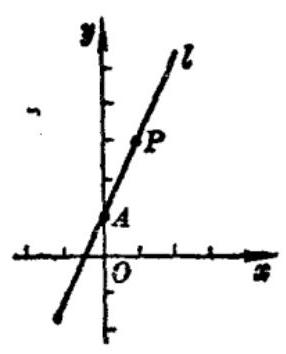
\includegraphics[max width=0.3\textwidth]{images/01912cc2-ffb6-728e-9ae7-b113ff05c64b_18_311691.jpg}
  %\documentclass[tikz, border=5pt]{standalone}
\begin{document}
	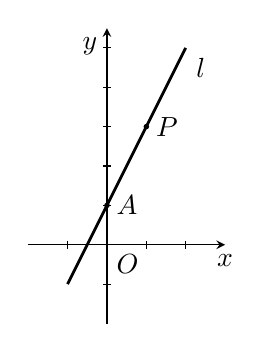
\begin{tikzpicture}[>=stealth, scale=0.5] % 箭头样式为stealth,
		
		% 绘制坐标轴
		\draw[->] (-2,0) -- (3,0) node[below] {$x$}; % x轴(带箭头和标签)
		\draw[->] (0,-2) -- (0,5.5) node[below left] {$y$}; % y轴(带箭头和标签)
		\node at (0,0) [below right] {$O$};           % 原点O的标签
		
		% 绘制所有小刻度线(从 -1 到 2,每隔 1 单位画竖线)
		\foreach \x in {-1,0,...,2} {
			\draw (\x, 0.1) -- (\x, -0.1);  % 小竖线(长 0.2 单位)
		}
		\foreach \y in {-1,0,...,5} {
			\draw (0.1,\y) -- (-0.1,\y);  % 小竖线(长 0.2 单位)
		}
		
		% 定义各关键点坐标
		\coordinate (A) at (0,1);  % 点A
		\coordinate (P) at (1,3); % 点P₂
		
		% 绘制直线l y=2x+1
		\draw[line width=1pt] (-1,-1) -- (2,5) node[below right]{$l$};
		
		% 标记各点的标签
		\fill (A) circle (2pt) node [right] {$A$};  % 带标签的实心点
		\fill (P) circle (2pt) node [right] {$P$};  % 带标签的实心点
		
	\end{tikzpicture}
\end{document}

  \caption{图 1-14}
\end{figure}

一般地,一次函数 \(y = {kx} + b\) 的图象是一条直线,它是以满足 \(y = {kx} + b\) 的每一对 \(x\text{、}y\) 的值为坐标的点构成的. 由于函数 \(y = {kx} + b\) 也可以看作二元一次方程,因此,我们也可以说, 这个方程的解和直线上的点也存在这样的一一对应关系.

\begin{corollary}[直线与方程的关系]
以一个方程的解为坐标的点都是某条直线上的点; 反之, 这条直线上点的坐标都是这个方程的解, 这时, 这个方程就叫做这条直线的方程, 这条直线叫做这个方程的直线.
\end{corollary}

在解析几何里研究直线时, 就是利用直线与方程的这种关系, 建立直线的方程, 并通过方程来研究直线的有关问题.

\begin{problemset}[练习]

\item 在坐标平面上, 画出下列方程的直线:

(1) \(y = x\) ; (2) \({2x} + {3y} = 6\) ;

(3) \({2x} + {3y} + 6 = 0\) ; (4) \({2x} - {3y} + 6 = 0\) .

\item (1) 用量角器测量上题中各直线向上的方向与 \(x\) 轴的正方向所成的角的度数;

(2) 量出各直线与 \(x\) 轴、 \(y\) 轴交点的坐标,并代入方程, 看它们是不是方程的解.
\end{problemset}

\section{直线的倾斜角和斜率}

为了建立直角坐标系中的直线方程, 需要研究直线的倾斜角和斜率.

\begin{definition}[倾斜角]
一条直线 \(l\) 向上的方向与 \(x\) 轴的正方向所成的最小正角叫做这条直线的倾斜角,如图 1-15 中的 \(\alpha\) .特别地,当直线 \(l\) 和 \(x\) 轴平行时,我们规定它的倾斜角为 \({0}^{ \circ }\) . 因此,倾斜角的取值范围是 \({0}^{ \circ } \leq \alpha < {180}^{ \circ }\) .
\end{definition}

\begin{figure}[h]
	\centering
	% 左侧图片:宽度设置为0.45倍文本宽度,预留间距
	\begin{subfigure}[h]{0.45\textwidth}
		\centering
		%  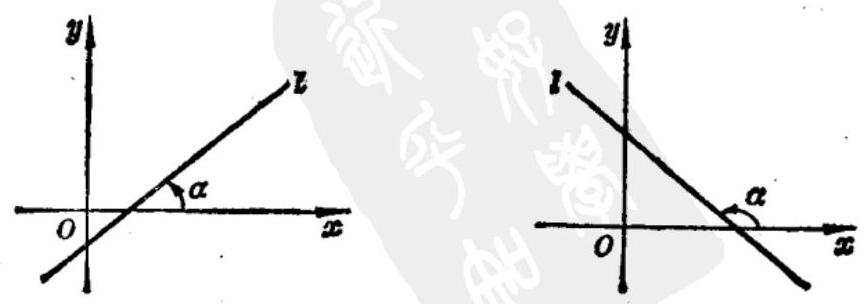
\includegraphics[max width=0.9\textwidth]{images/01912cc2-ffb6-728e-9ae7-b113ff05c64b_19_823562.jpg}
		%\documentclass[tikz, border=5pt]{standalone}
\begin{document}
	\begin{tikzpicture}[>=stealth, scale=0.8]
		% 绘制坐标轴
		\draw[->] (-2,0) -- (4,0) node[below] {$x$}; % x轴(带箭头和标签)
		\draw[->] (0,-2) -- (0,3) node[below left] {$y$}; % y轴(带箭头和标签)
		\node at (0,0) [below left] {$O$};           % 原点O的标签
		
		% 直线l y=x-1
		\draw[thick] (-1, -2) -- (3, 2) node[above right] {$l$};
		
		% 角度α(辅助线+角度标记)
		%	\draw[dashed] (1,0) -- (1, -0.5); % 垂直辅助线
		%	\pic[draw, angle radius=0.8cm, "$\alpha$"] % 绘制并标记角度
		%	{angle=(1,-0.5)--(1,0)--(-1,-1.5)};
		
		% x方向箭头(增强示意)
		\draw[->] (2, 0) arc (0:45:1) node[midway] {$\alpha$};
		
	\end{tikzpicture}
	
%	\begin{tikzpicture}[>=stealth, scale=0.8] % 箭头样式为stealth,
%		% 绘制坐标轴
%\draw[->] (-2,0) -- (4,0) node[below] {$x$}; % x轴(带箭头和标签)
%\draw[->] (0,-2) -- (0,3) node[below left] {$y$}; % y轴(带箭头和标签)
%\node at (0,0) [below left] {$O$};           % 原点O的标签
%
%% 直线l
%\draw[thick] (2.5, -1) -- (-1, 2) node[left] {$l$};
%
%% x方向箭头(增强示意)
%		\draw[->] (2, 0) arc (0:140:0.6) node[midway] {$\alpha$};
%		
%	\end{tikzpicture}

\end{document}

%		\caption{}
	\end{subfigure}
	\hfill % 两个图片之间添加空白填充,确保左右分布
	% 右侧图片:宽度设置为0.45倍文本宽度
	\begin{subfigure}[h]{0.45\textwidth}
		\centering
		%\documentclass[tikz, border=5pt]{standalone}
\begin{document}
%	\begin{tikzpicture}[>=stealth, scale=0.8]
%		% 绘制坐标轴
%		\draw[->] (-2,0) -- (4,0) node[below] {$x$}; % x轴(带箭头和标签)
%		\draw[->] (0,-2) -- (0,3) node[below left] {$y$}; % y轴(带箭头和标签)
%		\node at (0,0) [below left] {$O$};           % 原点O的标签
%		
%		% 直线l y=x-1
%		\draw[thick] (-1, -2) -- (3, 2) node[above right] {$l$};
%		
%		% 角度α(辅助线+角度标记)
%		%	\draw[dashed] (1,0) -- (1, -0.5); % 垂直辅助线
%		%	\pic[draw, angle radius=0.8cm, "$\alpha$"] % 绘制并标记角度
%		%	{angle=(1,-0.5)--(1,0)--(-1,-1.5)};
%		
%		% x方向箭头(增强示意)
%		\draw[->] (2, 0) arc (0:45:1) node[midway] {$\alpha$};
%		
%	\end{tikzpicture}
	
	\begin{tikzpicture}[>=stealth, scale=0.8] % 箭头样式为stealth,
		% 绘制坐标轴
\draw[->] (-2,0) -- (4,0) node[below] {$x$}; % x轴(带箭头和标签)
\draw[->] (0,-2) -- (0,3) node[below left] {$y$}; % y轴(带箭头和标签)
\node at (0,0) [below left] {$O$};           % 原点O的标签

% 直线l
\draw[thick] (2.5, -1) -- (-1, 2) node[left] {$l$};

% x方向箭头(增强示意)
		\draw[->] (2, 0) arc (0:140:0.6) node[midway] {$\alpha$};
		
	\end{tikzpicture}

\end{document}

%		\caption{}
	\end{subfigure}
	\caption{图 1-15}
\end{figure}

\begin{definition}[斜率]
  倾斜角不是 \({90}^{ \circ }\) 的直线,它的倾斜角的正切叫做这条直线的斜率. 直线的斜率常用 \(k\) 表示,即

\[
  k = \operatorname{tg}\alpha \text{or} k = \tan\alpha  \text{.}
\]

倾斜角是 \({90}^{ \circ }\) 的直线没有斜率; 倾斜角不是 \({90}^{ \circ }\) 的直线, 都有斜率, 并且是确定的, 我们常用斜率来表示倾斜角不等于 \({90}^{ \circ }\) 的直线对于 \(x\) 轴的倾斜程度.
\end{definition}

在坐标平面上,如果已知两点 \({P}_{1}\left( {{x}_{1},{y}_{1}}\right) \text{、}{P}_{2}\left( {{x}_{2},{y}_{2}}\right)\) ,那么直线 \({P}_{1}{P}_{2}\) 就是确定的,当直线 \({P}_{1}{P}_{2}\) 的倾斜角不等于 \({90}^{ \circ }\) 时, 这条直线的斜率也是确定的. 下面我们来研究怎样用两点的坐标来表示直线 \({P}_{1}{P}_{2}\) 的斜率.

设直线 \({P}_{1}{P}_{2}\) 的倾斜角是 \(\alpha\) ,斜率是 \(k,\overline{{P}_{1}{P}_{2}}\) 的方向是向上的方向. 从 \({P}_{1}\text{、}{P}_{2}\) 分别向 \(x\) 轴作垂线 \({P}_{1}{M}_{1}\text{、}{P}_{2}{M}_{2}\) ,再作 \({P}_{1}Q \bot {P}_{2}{M}_{2}\) ,垂足分别是 \({M}_{1}\text{、}{M}_{2}\text{、}Q\) . 那么

\[
  \alpha = \angle Q{P}_{1}{P}_{2}\text{ (图 1-16 甲),} 
\]
或 \(\alpha = \angle P{P}_{1}{P}_{2}\)  (图 1-16 乙).
\begin{figure}[h]
	\centering
	% 左侧图片:宽度设置为0.45倍文本宽度,预留间距
	\begin{subfigure}[h]{0.45\textwidth}
		\centering
%		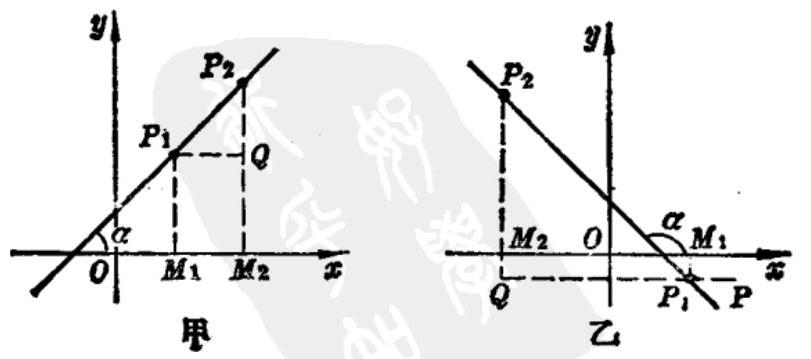
\includegraphics[max width=0.8\textwidth]{images/01912cc2-ffb6-728e-9ae7-b113ff05c64b_20_458905.jpg}
		%\documentclass[tikz, border=5pt]{standalone}
\begin{document}
	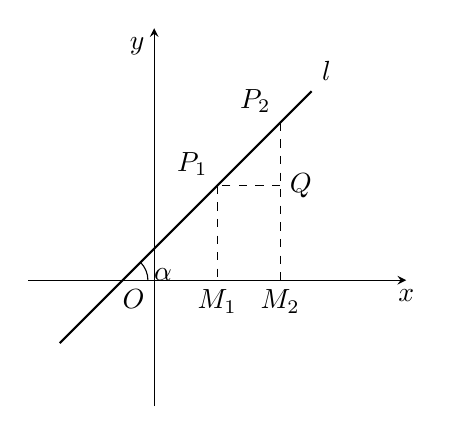
\begin{tikzpicture}[>=stealth, scale=0.8]
		% 绘制坐标轴
		\draw[->] (-2,0) -- (4,0) node[below] {$x$}; % x轴(带箭头和标签)
		\draw[->] (0,-2) -- (0,4) node[below left] {$y$}; % y轴(带箭头和标签)
		\node at (0,0) [below left] {$O$};           % 原点O的标签
		
		% 直线l y=x+0.5
		\draw[thick] (-1.5, -1) -- (2.5, 3) node[above right] {$l$}; 
		
		% 定义各关键点坐标
		\coordinate (P1) at (1,1.5);  % 点P₁
		\coordinate (P2) at (2,2.5); % 点P₂
		\coordinate (M1) at (1,0);  % 点M₁
		\coordinate (M2) at (2,0); % 点M₂
		\coordinate (Q)  at (2,1.5);% 点Q
		
		% 绘制虚线辅助线(矩形的边)
		\draw[dashed] (Q) -- (P1);  % Q到P₁的虚线
		\draw[dashed] (P1) -- (M1); % P₁到x轴的虚线
		\draw[dashed] (P2) -- (M2); % P₂到y轴的虚线
		
		% 标记各点的标签
		\node at (P1) [above left]  {$P_1$};
		\node at (P2) [above left]      {$P_2$};
		\node at (M1) [below]          {$M_1$};
		\node at (M2) [below] {$M_2$};
		\node at (Q)  [right]   {$Q$};
		
		%  弧线
		\draw (-0.1, 0) arc (0:45:0.4) ; 
		node[above right] at (0,0) {$\alpha$}; 
		
	\end{tikzpicture}
	
%	\begin{tikzpicture}[>=stealth, scale=0.8] % 箭头样式为stealth,
%		% 绘制坐标轴
%		\draw[->] (-3,0) -- (3,0) node[below] {$x$}; % x轴(带箭头和标签)
%		\draw[->] (0,-1.5) -- (0,4.5) node[below left] {$y$}; % y轴(带箭头和标签)
%		\node at (0,0) [above left] {$O$};           % 原点O的标签
%		
%		% 直线l  y=-x+1
%		\draw[thick] (2, -1) -- (-2.5, 3.5) node[below left] {$l$}; 
%		
%		% 定义各关键点坐标
%		\coordinate (P1) at (1.5,-0.5);  % 点P₁
%		\coordinate (P2) at (-2,3); % 点P₂
%		\coordinate (M1) at (1.5,0);  % 点M₁
%		\coordinate (M2) at (-2,0); % 点M₂
%		\coordinate (Q)  at (-2,-0.5);% 点Q
%		\coordinate (P) at (2.5,-0.5);  % 点P
%		
%		% 绘制虚线辅助线(矩形的边)
%		\draw[dashed] (Q) -- (P);  % Q到P₁的虚线
%		\draw[dashed] (P1) -- (M1); % P₁到x轴的虚线
%		\draw[dashed] (P2) -- (Q); % P₂到y轴的虚线
%		
%		% 标记各点的标签
%		\node at (P) [below]  {$P$};
%		\node at (P1) [below]  {$P_1$};
%		\node at (P2) [right]   {$P_2$};
%		\node at (M1) [above right]  {$M_1$};
%		\node at (M2) [above left]  {$M_2$};
%		\node at (Q)  [below]   {$Q$};
%		
%		%  弧线
%		\draw (1.4, 0) arc (0:135:0.4) node[midway] {$\alpha$}; 
%		
%	\end{tikzpicture}
	
\end{document}

		\caption{甲}
	\end{subfigure}
	\hfill % 两个图片之间添加空白填充,确保左右分布
	% 右侧图片:宽度设置为0.45倍文本宽度
	\begin{subfigure}[h]{0.45\textwidth}
		\centering
		%\documentclass[tikz, border=5pt]{standalone}
\begin{document}
%	\begin{tikzpicture}[>=stealth, scale=0.8]
%		% 绘制坐标轴
%		\draw[->] (-2,0) -- (4,0) node[below] {$x$}; % x轴(带箭头和标签)
%		\draw[->] (0,-2) -- (0,4) node[below left] {$y$}; % y轴(带箭头和标签)
%		\node at (0,0) [below left] {$O$};           % 原点O的标签
%		
%		% 直线l y=x+0.5
%		\draw[thick] (-1.5, -1) -- (2.5, 3) node[above right] {$l$}; 
%		
%		% 定义各关键点坐标
%		\coordinate (P1) at (1,1.5);  % 点P₁
%		\coordinate (P2) at (2,2.5); % 点P₂
%		\coordinate (M1) at (1,0);  % 点M₁
%		\coordinate (M2) at (2,0); % 点M₂
%		\coordinate (Q)  at (2,1.5);% 点Q
%		
%		% 绘制虚线辅助线(矩形的边)
%		\draw[dashed] (Q) -- (P1);  % Q到P₁的虚线
%		\draw[dashed] (P1) -- (M1); % P₁到x轴的虚线
%		\draw[dashed] (P2) -- (M2); % P₂到y轴的虚线
%		
%		% 标记各点的标签
%		\node at (P1) [above left]  {$P_1$};
%		\node at (P2) [above left]      {$P_2$};
%		\node at (M1) [below]          {$M_1$};
%		\node at (M2) [below] {$M_2$};
%		\node at (Q)  [right]   {$Q$};
%		
%		%  弧线
%		\draw (-0.1, 0) arc (0:45:0.4) ; 
%		node[above right] at (0,0) {$\alpha$}; 
%		
%	\end{tikzpicture}
	
	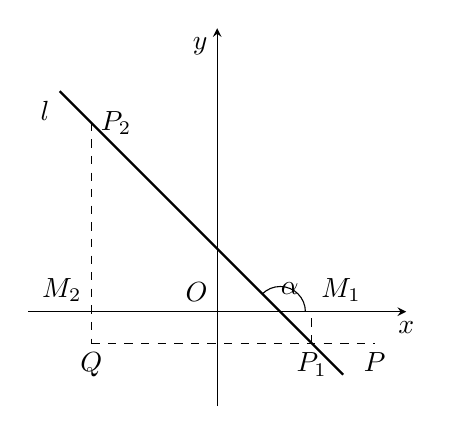
\begin{tikzpicture}[>=stealth, scale=0.8] % 箭头样式为stealth,
		% 绘制坐标轴
		\draw[->] (-3,0) -- (3,0) node[below] {$x$}; % x轴(带箭头和标签)
		\draw[->] (0,-1.5) -- (0,4.5) node[below left] {$y$}; % y轴(带箭头和标签)
		\node at (0,0) [above left] {$O$};           % 原点O的标签
		
		% 直线l  y=-x+1
		\draw[thick] (2, -1) -- (-2.5, 3.5) node[below left] {$l$}; 
		
		% 定义各关键点坐标
		\coordinate (P1) at (1.5,-0.5);  % 点P₁
		\coordinate (P2) at (-2,3); % 点P₂
		\coordinate (M1) at (1.5,0);  % 点M₁
		\coordinate (M2) at (-2,0); % 点M₂
		\coordinate (Q)  at (-2,-0.5);% 点Q
		\coordinate (P) at (2.5,-0.5);  % 点P
		
		% 绘制虚线辅助线(矩形的边)
		\draw[dashed] (Q) -- (P);  % Q到P₁的虚线
		\draw[dashed] (P1) -- (M1); % P₁到x轴的虚线
		\draw[dashed] (P2) -- (Q); % P₂到y轴的虚线
		
		% 标记各点的标签
		\node at (P) [below]  {$P$};
		\node at (P1) [below]  {$P_1$};
		\node at (P2) [right]   {$P_2$};
		\node at (M1) [above right]  {$M_1$};
		\node at (M2) [above left]  {$M_2$};
		\node at (Q)  [below]   {$Q$};
		
		%  弧线
		\draw (1.4, 0) arc (0:135:0.4) node[midway] {$\alpha$}; 
		
	\end{tikzpicture}
	
\end{document}

		\caption{乙}
	\end{subfigure}
	\caption{图 1-16}
\end{figure}

在图 1-16 甲中,

\[
  \operatorname{tg}\alpha = \operatorname{tg}Q{P}_{1}{P}_{2} = \frac{Q{P}_{2}}{{P}_{1}Q} = \frac{{y}_{2} - {y}_{1}}{{x}_{2} - {x}_{1}}.
\]

在图 1-16 乙中,

\[
  \operatorname{tg}\alpha = \operatorname{tg}P{P}_{1}{P}_{2} = \frac{Q{P}_{2}}{{P}_{1}Q} = \frac{{y}_{2} - {y}_{1}}{{x}_{2} - {x}_{1}}.
\]

同样,对于 \(\overline{{P}_{2}{P}_{1}}\) 方向向上的情形,

\[
  \operatorname{tg}\alpha = \frac{{y}_{1} - {y}_{2}}{{x}_{1} - {x}_{2}} = \frac{{y}_{2} - {y}_{1}}{{x}_{2} - {x}_{1}}.
\]

\begin{corollary}[直线上两点的斜率公式]
综上所述,我们得到经过点 \({P}_{1}\left( {{x}_{1},{y}_{1}}\right) \text{、}{P}_{2}\left( {{x}_{2},{y}_{2}}\right)\) 两点的直线的斜率公式:

\[
  \mathbf{k} = \frac{{\mathbf{y}}_{2} - {\mathbf{y}}_{1}}{{\mathbf{x}}_{2} - {\mathbf{x}}_{1}}.
\]
\end{corollary}

\begin{figure}[h]
  \centering
%  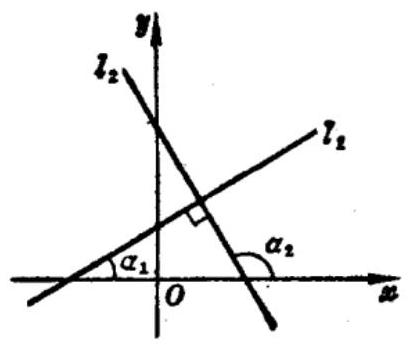
\includegraphics[max width=0.4\textwidth]{images/01912cc2-ffb6-728e-9ae7-b113ff05c64b_21_706247.jpg}
  %\documentclass[tikz, border=5pt]{standalone}
\usetikzlibrary{angles, quotes, shapes.geometric} % 加载角度、引用、直角标记库

\begin{document}
	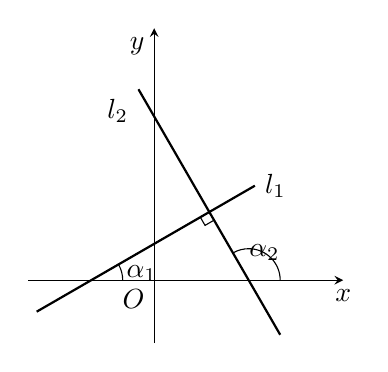
\begin{tikzpicture}[>=stealth, scale=0.8]

    % 1. 绘制坐标轴
    \draw[->] (-2,0) -- (3,0) node[below] {$x$}; % x轴(带箭头和标签)
    \draw[->] (0,-1) -- (0,4) node[below left] {$y$}; % y轴(带箭头和标签)
    \node at (0,0) [below left] {$O$}; % 原点标记

    % 2. 绘制直线 \( l_1 \)(倾斜向上)
    \draw[thick] (-1, 0) --  ++(30: 3) node[right] {$l_1$};
    \draw[thick] (-1, 0) --  ++(-150: 1) ;
    
    % 3. 绘制直线 \( l_2 \)(倾斜向下,与 \( l_1 \) 垂直)
    \draw[thick] (1.5, 0) -- ++(120: 3.5) node[below left] {$l_2$};
    \draw[thick] (1.5, 0) -- ++(-60: 1) ;
    
    % 4. 标记角度 \( \alpha_1 \)(\( l_1 \) 与 x 轴正方向的锐角)
    \draw (-0.5, 0) arc (0:30:0.5) ;
    \node at (-0.2, 0.1) []  {$\alpha_1$}; 

    % 5. 标记角度 \( \alpha_2 \)(\( l_2 \) 与 x 轴正方向的钝角)
    \draw (2, 0) arc (0:120:0.5) node[midway] {$\alpha_2$}; 
    
    % 6. 绘制直角标记(两直线垂直的符号)
    \draw (-1, 0) --  ++(30: 2) -- ++(-60: 0.15) -- ++(30: 0.15) ;

	\end{tikzpicture}
\end{document}

  \caption{图 1-17}
\end{figure}



例 1 如图 1-17,直线 \({l}_{1}\) 的倾斜角 \({\alpha }_{1} = {30}^{ \circ }\) ,直线 \({l}_{2} \bot {l}_{1}\) . 求 \({l}_{1}\text{、}{l}_{2}\) 的斜率.

解: \({l}_{1}\) 的斜率 \({k}_{1} = \operatorname{tg}{30}^{ \circ } = \frac{\sqrt{3}}{3}\) ,

\(\because {l}_{2}\) 的倾斜角 \({\alpha }_{2} = {90}^{ \circ } + {30}^{ \circ } = {120}^{ \circ }\) ,

\(\therefore {l}_{2}\) 的斜率 \({k}_{2} = \operatorname{tg}{120}^{ \circ } = - \operatorname{tg}{60}^{ \circ } = - \sqrt{3}\) .

例 2 求经过 \(A\left( {-2,0}\right) \text{、}B\left( {-5,3}\right)\) 两点的直线的斜率和倾斜角.

解:

\[
  k = \frac{3 - 0}{-5 - \left( {-2}\right) } = - 1,
\]

就是

\[
  \operatorname{tg}\alpha = - 1\text{. }
\]

..

\[
    {0}^{ \circ } \leq \alpha < {180}^{ \circ }
\]

\[
  \therefore \;\alpha = {135}^{ \circ }\text{. }
\]

因此,这条直线的斜率是 -1,倾斜角是 \({135}^{ \circ }\) .

\begin{problemset}[练习]

\item 已知直线的倾斜角, 讨论这条直线的斜率的值:

(1) \(\alpha = {0}^{ \circ }\) ; (2) \({0}^{ \circ } < \alpha < {90}^{ \circ }\) ;

(3) \(\alpha = {90}^{ \circ }\) ; (4) \({90}^{ \circ } < \alpha < {180}^{ \circ }\) .

\item 求经过下列每两个点的直线的斜率和倾斜角:

(1) \(C\left( {{10},8}\right) \text{、}D\left( {4, - 4}\right)\) ;

(2) \(P\left( {0,0}\right) \text{、}Q\left( {-1,\sqrt{3}}\right)\) ;

(3) \(M\left( {-\sqrt{3},\sqrt{2}}\right) \text{、}N\left( {-\sqrt{2},\sqrt{3}}\right)\) .

\item 已知: \(a\text{、}b\text{、}c\) 是两两不等的实数. 求经过下列每两个点的直线的倾斜角:

(1) \(A\left( {a,c}\right) \text{、}B\left( {b,c}\right)\) ; (2) \(C\left( {a,b}\right) \text{、}D\left( {a,c}\right)\) ;

(3) \(P\left( {b,b + c}\right) \text{、}Q\left( {a,c + a}\right)\) .

\item 证明: 已知三点 \(A\text{、}B\text{、}C\) . 如果直线 \({AB}\text{、}{AC}\) 的斜率相同. 那么这三点在同一条直线上.
\end{problemset}

\section{直线方程的几种形式}

一条直线在直角坐标平面内的位置, 可以由不同的条件来确定. 下面, 我们来研究怎样根据所给的条件, 求出直线的方程.

\section*{1. 点斜式}

已知直线 \(l\) 的斜率是 \(k\) ,并且经过点 \({P}_{1}\left( {{x}_{1},{y}_{1}}\right)\) ,求直线 \(l\) 的方程 (图 1-18).

设点 \(P\left( {x,y}\right)\) 是直线 \(l\) 上不同于点 \({P}_{1}\) 的任意一点. 根据经过两点的直线的斜率公式, 得

\[
  k = \frac{y - {y}_{1}}{x - {x}_{1}}
\]

可化为

\begin{corollary}[点斜式]
\[
  y - {y}_{1} = k\left( {x - {x}_{1}}\right) .
\]
\end{corollary}

\begin{figure}[h]
	\centering
	% 左侧图片:宽度设置为0.45倍文本宽度,预留间距
	\begin{subfigure}[h]{0.45\textwidth}
		\centering
%		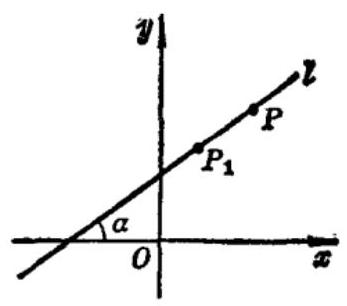
\includegraphics[max width=0.4\textwidth]{images/01912cc2-ffb6-728e-9ae7-b113ff05c64b_23_507928.jpg}
		%\documentclass[tikz, border=5pt]{standalone}
\begin{document}
	\begin{tikzpicture}[>=stealth, scale=0.8]
		% 绘制坐标轴
		\draw[->] (-2,0) -- (3,0) node[below] {$x$}; % x轴(带箭头和标签)
		\draw[->] (0,-1) -- (0,4) node[below left] {$y$}; % y轴(带箭头和标签)
		\node at (0,0) [below left] {$O$};           % 原点O的标签
		
		% 直线l y=x+1
		\draw[thick] (-1.5, -0.5) -- (2, 3) node[below right] {$l$}; 
		
		% 标记各点的标签
		\fill (0.5,1.5) circle (2pt) node[below] {$P_1$};  % 点P_1
		\fill (1.5,2.5) circle (2pt) node[below] {$P$};       % 点P
		
		%  弧线
		\draw (-0.5, 0) arc (0:45:0.5) ; 
		\node[above right] at (-0.5,0) {$\alpha$}; 
		
	\end{tikzpicture}
	
\end{document}

		\caption{图 1-18}
	\end{subfigure}
	\hfill % 两个图片之间添加空白填充,确保左右分布
	% 右侧图片:宽度设置为0.45倍文本宽度
	\begin{subfigure}[h]{0.45\textwidth}
		\centering
%		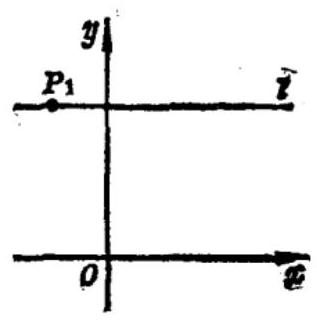
\includegraphics[max width=0.3\textwidth]{images/01912cc2-ffb6-728e-9ae7-b113ff05c64b_23_669751.jpg}
		%\documentclass[tikz, border=5pt]{standalone}
\begin{document}
	\begin{tikzpicture}[>=stealth, scale=0.8]
		% 绘制坐标轴
		\draw[->] (-2,0) -- (3,0) node[below] {$x$}; % x轴(带箭头和标签)
		\draw[->] (0,-1) -- (0,4) node[below left] {$y$}; % y轴(带箭头和标签)
		\node at (0,0) [below left] {$O$};           % 原点O的标签
		
		% 直线l y=2.5
		\draw[thick] (-1.5, 2.5) -- (2.5, 2.5) node[below right] {$l$}; 
		
		% 标记各点的标签
		\fill (-0.5,2.5) circle (2pt) node[below] {$P_1$};  % 点P_1
		
	\end{tikzpicture}
	
\end{document}

		\caption{图 1-19}
	\end{subfigure}
%	\caption{}
\end{figure}

可以验证,直线 \(l\) 上的每个点的坐标都是这个方程的解; 反过来,以这个方程的解为坐标的点都在直线 \(l\) 上,所以这个方程就是过点 \({P}_{1}\) 、斜率为 \(k\) 的直线 \(l\) 的方程.

这个方程是由直线上一点和直线的斜率确定的, 叫做直线方程的点斜式.

当直线 \(l\) 的倾斜角为 \({0}^{ \circ }\) 时 (图 1-19), \(\operatorname{tg}{0}^{ \circ } = 0\) ,即 \(k = 0\) . 这时直线 \(l\) 的方程就是

\[
  y = {y}_{1}
\]

当直线 \(l\) 的倾斜角为 \({90}^{ \circ }\) 时,直线没有斜率,这时直线 \(l\) 与 \(y\) 轴平行或重合,它的方程不能用点斜式表示. 但因 \(l\) 上

每一点的横坐标都等于 \({x}_{1}\) (图 1-20),所以它的方程是

\[
  x = {x}_{1}
\]

\begin{figure}[h]
	\centering
	% 左侧图片:宽度设置为0.45倍文本宽度,预留间距
	\begin{subfigure}[h]{0.45\textwidth}
		\centering
%		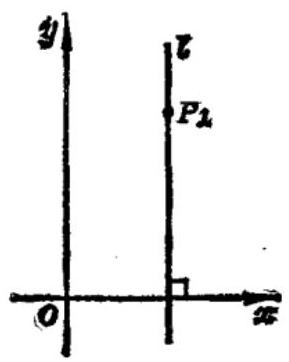
\includegraphics[max width=0.3\textwidth]{images/01912cc2-ffb6-728e-9ae7-b113ff05c64b_24_697633.jpg}
		%\documentclass[tikz, border=5pt]{standalone}
\begin{document}
	\begin{tikzpicture}[>=stealth, scale=0.8]
		% 绘制坐标轴
		\draw[->] (-1,0) -- (3,0) node[below] {$x$}; % x轴(带箭头和标签)
		\draw[->] (0,-1) -- (0,4) node[below left] {$y$}; % y轴(带箭头和标签)
		\node at (0,0) [below left] {$O$};           % 原点O的标签
		% 直线l x=2
		\draw[thick] (2, -0.5) -- (2, 3.5) node[below right] {$l$}; 
		% 标记各点的标签
		\fill (2,2.5) circle (2pt) node[left] {$P_1$};  % 点P_1
	\end{tikzpicture}
\end{document}

		\caption{图 1-20}
	\end{subfigure}
	\hfill % 两个图片之间添加空白填充,确保左右分布
	% 右侧图片:宽度设置为0.45倍文本宽度
	\begin{subfigure}[h]{0.45\textwidth}
		\centering
%		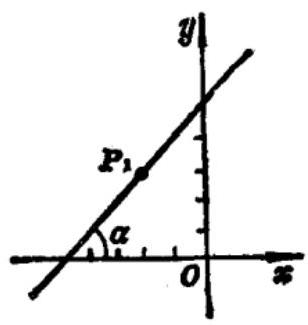
\includegraphics[max width=0.3\textwidth]{images/01912cc2-ffb6-728e-9ae7-b113ff05c64b_24_594823.jpg}
		%\documentclass[tikz, border=5pt]{standalone}
\begin{document}
	\begin{tikzpicture}[>=stealth, scale=0.8]
		% 绘制坐标轴
		\draw[->] (-3.5,0) -- (1.5,0) node[below] {$x$}; % x轴(带箭头和标签)
		\draw[->] (0,-1) -- (0,4) node[below left] {$y$}; % y轴(带箭头和标签)
		\node at (0,0) [below left] {$O$};           % 原点O的标签
		% 直线l y=x+2.5
		\draw[thick] (-3, -0.5) -- (1, 3.5) node[below right] {$l$}; 
		% 绘制所有小刻度线(从 -1 到 2,每隔 1 单位画竖线)
		\foreach \x in {-2, -1.5,...,-0.5} {
			\draw (\x, 0.1) -- (\x, -0.1);  % 小竖线(长 0.2 单位)
		}
		\foreach \y in {0.5,1,...,2} {
			\draw (0.1,\y) -- (-0.1,\y);  % 小竖线(长 0.2 单位)
		}
		% 标记各点的标签
		\fill (-1,1.5) circle (2pt) node[below] {$P_1$};  % 点P_1
		%  弧线
		\draw (-2, 0) arc (0:45:0.5) node [midway] {$\alpha$}; 
%		\node[above right] at (-0.5,0) {$\alpha$}; 
	\end{tikzpicture}
\end{document}

		\caption{图 1-21}
	\end{subfigure}
	%	\caption{}
\end{figure}

例 1 一条直线经过点 \({P}_{1}\left( {-2,3}\right)\) ,倾斜角 \(\alpha = {45}^{ \circ }\) . 求这条直线的方程, 并画出图形.

解: 这条直线经过点 \({P}_{1}\left( {-2,3}\right)\) ,斜率是

\[
  k = \operatorname{tg}{45}^{ \circ } = 1\text{. }
\]

代入点斜式, 得

\[
  y - 3 = x + 2,
\]

即

\[
  x - y + 5 = 0.
\]

这就是所求的直线方程, 图形如图 1-21.

如果已知直线 \(l\) 的斜率是 \(k\) ,与 \(y\) 轴的交点是 \(\left( {0,b}\right) (b\) 是直线 \(l\) 在 \(y\) 轴上的截距),代入点斜式得直线 \(l\) 的方程:

\[
  y - b = k\left( {x - 0}\right) \text{. }
\]

也就是
\begin{corollary}[斜截式]
\[
  y = {kx} + b\text{. }
\]
\end{corollary}
这个方程是由直线 \(l\) 的斜率和它在 \(y\) 轴上的截距确定的, 所以叫做直线方程的斜截式.

\begin{problemset}[练习]

\item 写出下列直线的点斜式方程, 并画出图形:

(1) 经过点 \(A\left( {2,5}\right)\) ,斜率是 4 ;

(2)经过点 \(B\left( {3, - 1}\right)\) ,斜率是 \(\sqrt{2}\) ;

(3)经过点 \(C\left( {-\sqrt{2},2}\right)\) ,倾斜角是 \({30}^{ \circ }\) ;

(4)经过点 \(D\left( {0,3}\right)\) ,倾斜角是 \({0}^{ \circ }\) ;

(5) 经过点 \(E\left( {4, - 2}\right)\) ,倾斜角是 \({120}^{ \circ }\) .

\item 已知下列直线的点斜式方程, 求各直线经过的已知点、直线的斜率和倾斜角:


(1) \(y - 2 = x - 1\) ; (2) \(y - 3 = \sqrt{3}\left( {x - 4}\right)\) ;


(3) \(y + 3 = - \left( {x - 1}\right)\) ; (4) \(y + 2 = - \frac{\sqrt{3}}{3}\left( {x + 1}\right)\) .

\item 写出下列直线的斜截式方程:

(1)斜率是 \(\frac{\sqrt{3}}{2},y\) 轴上的截距是 -2 ;

(2)倾斜角是 \({135}^{ \circ },y\) 轴上的截距是 3 。
\end{problemset}

\section*{2. 两点式}

已知直线 \(l\) 经过两点 \({P}_{1}\left( {{x}_{1},{y}_{1}}\right) \text{、}{P}_{2}\left( {{x}_{2},{y}_{2}}\right) \left( {{x}_{1} \neq {x}_{2}}\right)\) ,求直线 \(l\) 的方程.

因为直线 \(l\) 经过点 \({P}_{1}\left( {{x}_{1},{y}_{1}}\right) \text{、}{P}_{2}\left( {{x}_{2},{y}_{2}}\right)\) ,并且 \({x}_{1} \neq {x}_{2}\) ,所以它的斜率 \(k = \frac{{y}_{2} - {y}_{1}}{{x}_{2} - {x}_{1}}\) . 代入点斜式,得

\[
  y - {y}_{1} = \frac{{y}_{2} - {y}_{1}}{{x}_{2} - {x}_{1}}\left( {x - {x}_{1}}\right) .
\]
\begin{corollary}[两点式]
当 \({y}_{2} \neq {y}_{1}\) 时,方程可以写成:

\[
  \frac{y - {y}_{1}}{{y}_{2} - {y}_{1}} = \frac{x - {x}_{1}}{{x}_{2} - {x}_{1}}
\]

这个方程是由直线上两点确定的, 叫做直线方程的两点式.
\end{corollary}
例 2 已知直线 \(l\) 在 \(x\) 轴和 \(y\) 轴上的截距分别是 \(a\) 和 \(b\) \(\left( {a \neq 0,b \neq 0}\right)\) ,求直线 \(l\) 的方程.

解: 因为直线 \(l\) 经过 \(A\left( {a,0}\right)\) 和 \(B\left( {0,b}\right)\) 两点,将这两点的坐标代入两点式, 得

\[
  \frac{y - 0}{b - 0} = \frac{x - a}{0 - a}
\]

就是
\begin{corollary}[截距式]
\[
  \frac{x}{a} + \frac{y}{b} = 1
\]

这个方程是由直线在 \(x\) 轴和 \(y\) 轴上的截距确定的,叫做直线方程的截距式.
\end{corollary}
例 3 三角形的顶点是 \(A\left( {-5,0}\right) \text{、}B\left( {3, - 3}\right) \text{、}C\left( {0,2}\right)\) (图 1-22), 求这个三角形三边所在直线的方程.

解: 直线 \({AB}\) 过 \(A\left( {-5,0}\right)\) 、 \(B\left( {3, - 3}\right)\) 两点. 由两点式得

\[
  \frac{y - 0}{-3 - 0} = \frac{x - \left( {-5}\right) }{3 - \left( {-5}\right) }
\]

\begin{figure}[h]
  \centering
%  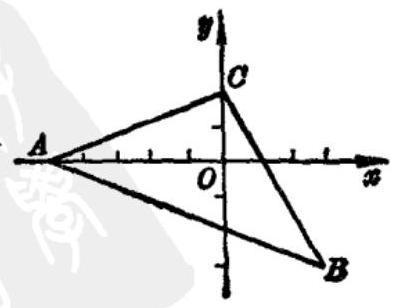
\includegraphics[max width=0.4\textwidth]{images/01912cc2-ffb6-728e-9ae7-b113ff05c64b_26_981074.jpg}
  %\documentclass[tikz, border=5pt]{standalone}
\begin{document}
	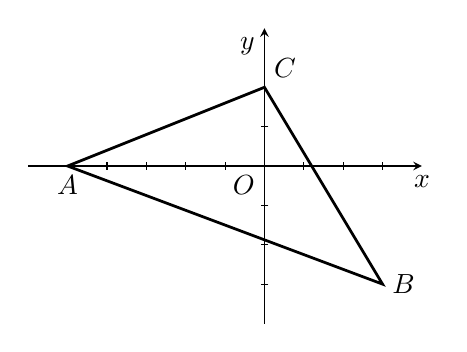
\begin{tikzpicture}[>=stealth, scale=0.5]
		% 绘制坐标轴
		\draw[->] (-6,0) -- (4,0) node[below] {$x$}; % x轴(带箭头和标签)
		\draw[->] (0,-4) -- (0,3.5) node[below left] {$y$}; % y轴(带箭头和标签)
		\node at (0,0) [below left] {$O$};           % 原点O的标签

		% 绘制所有小刻度线(从 -1 到 2,每隔 1 单位画竖线)
		\foreach \x in {-4, -3,...,3} {
			\draw (\x, 0.1) -- (\x, -0.1);  % 小竖线(长 0.2 单位)
		}
		\foreach \y in {-3,-2,...,1} {
			\draw (0.1,\y) -- (-0.1,\y);  % 小竖线(长 0.2 单位)
		}
		
		% 定义各关键点坐标(可根据图形比例调整)
		\coordinate (A) at (-5,0);   % 点 $A$
		\coordinate (B)  at (3,-3);    % 点 $B$
		\coordinate (C) at (0,2);    % 点 $C$
		
		% 绘制连线
		\draw [line width=1pt] (A) -- (B) -- (C) -- cycle; % 绘制三角形
		
		% 标记各点的标签 实心圆点
%		\fill (G) circle (2pt) node [right] {$G$};  % 带标签的实心点
		\node at (A) [below] {$A$}; 
		\node at (B) [right] {$B$}; 
		\node at (C) [above right] {$C$}; 
		
	\end{tikzpicture}
\end{document}

  \caption{图 1-22}
\end{figure}

即

\[
    {3x} + {8y} + {15} = 0.
\]

这就是直线 \({AB}\) 的方程.

直线 \({BC}\) 在 \(y\) 轴上的截距是 2,斜率是

\[
  k = \frac{2 - \left( {-3}\right) }{0 - 3} = - \frac{5}{3}.
\]

由斜截式得

\[
  y = - \frac{5}{3}x + 2
\]

即

\[
    {5x} + {3y} - 6 = 0\text{. }
\]

这就是直线 \({BC}\) 的方程.

直线 \({AC}\) 在 \(x\) 轴、 \(y\) 轴上的截距分别是 -5、2 . 由截距式得

\[
  \frac{x}{-5} + \frac{y}{2} = 1
\]

即

\[
    {2x} - {5y} + {10} = 0\text{. }
\]

这就是直线 \({AC}\) 的方程.

\begin{problemset}[练习]

\item 在什么情况下直线方程可以表示成下列形式:

(1) 点斜式; (2) 斜截式; (3) 两点式; (4) 截距式.

\item 求过下列两点的直线的两点式方程, 再化成斜截式方程:

(1) \({P}_{1}\left( {2,1}\right) \text{、}{P}_{2}\left( {0, - 3}\right)\) ;

(2) \(A\left( {0,5}\right) \text{、}B\left( {5,0}\right)\) ;

(3) \(C\left( {-4, - 5}\right) \text{、}D\left( {0,0}\right)\) .

\item 写出下列直线的截距式方程, 并根据截距式方程作出直线:

(1) \(x\) 轴上的截距是 \(2,y\) 轴上的截距是 3 ;

(2) \(x\) 轴上的截距是 \(- 5,y\) 轴上的截距是 6 ;

(3) \(x\) 轴上的截距是 \(4,y\) 轴上的截距是 -3 ;

(4) \(x\) 轴上的截距和 \(y\) 轴上的截距都是 \(- \frac{1}{2}\) .
\end{problemset}

\section{直线方程的一般形式}

上一节我们学习了直线方程的几种特殊形式, 它们都是二元一次方程. 下面我们来进一步研究直线和二元一次方程的关系.

我们知道,在直角坐标系中,每一条直线都有倾斜角 \(\alpha\) . 当 \(\alpha \neq {90}^{ \circ }\) 时,它们都有斜率,方程可写成下面的形式:

\[
  y = {kx} + b
\]

当 \(\alpha = {90}^{ \circ }\) 时,它的方程可以写成 \(x = {x}_{1}\) 的形式. 由于是在坐标平面上讨论问题,所以这个方程应认为是关于 \(x\text{、}y\) 的二元一次方程,其中 \(y\) 的系数是 0 .

这样, 对于每一条直线都可以求得它的方程, 而且是二元一次方程. 就是说,直线的方程都是关于 \(x\text{、}y\) 的一次方程.
\begin{corollary}[直线方程的一般形式]
下面证明,任何关于 \(x\text{、}y\) 的一次方程都表示一条直线.

\(x\text{、}y\) 的一次方程的一般形式是

\[
    {Ax} + {By} + C = 0, \tag{1}
\]
\end{corollary}
其中 \(A\text{、}B\) 不同时为零. 下面分 \(B \neq 0\) 和 \(B = 0\) 两种情况加以研究.

(i) 当 \(B \neq 0\) 时,方程 (1) 可化为

\[
  y = - \frac{A}{B}x - \frac{C}{B}.
\]

这就是直线的斜截式方程,它表示斜率为 \(- \frac{A}{B}\) 、在 \(y\) 轴上的截距为 \(- \frac{C}{B}\) 的直线.

(ii) 当 \(B = 0\) 时,由于 \(A\text{、}B\) 不同时为零,必有 \(A \neq 0\) ,方程 (1) 可化为

\[
  x = - \frac{C}{A}
\]

它表示一条与 \(y\) 轴平行或重合的直线.

根据以上的讨论, 我们又得到下面的结论:

关于 \(x\) 和 \(y\) 的一次方程都表示一条直线.

我们把方程

\[
  \mathbf{A}\mathbf{x} + \mathbf{B}\mathbf{y} + \mathbf{C} = \mathbf{0}. \tag{1}
\]

(其中 \(A\text{、}B\) 不全为零) 叫做直线方程的一般式.

例 1 已知直线经过点 \(A\left( {6, - 4}\right)\) ,斜率为 \(- \frac{4}{3}\) ,求直线的 (1) 点斜式; (2) 一般式; (3) 截距式.

解: 经过点 \(A\left( {6, - 4}\right)\) 并且斜率等于 \(- \frac{4}{3}\) 的直线的点斜式是

\[
  y + 4 = - \frac{4}{3}\left( {x - 6}\right)
\]

化成一般式, 得

\[
    {4x} + {3y} - {12} = 0.
\]

把常数项移到等号的右边, 再把方程的两边都除以 12 , 就得截距式

\[
  \frac{x}{3} + \frac{y}{4} = 1
\]

例 2 把直线 \(l\) 的方程 \(x - {2y} + 6 = 0\) 化成斜截式,求出直线 \(l\) 的斜率和在 \(x\) 轴与 \(y\) 轴上的截距,并画图.

解: 将原方程移项,得 \({2y} = x + 6\) . 两边除以 2,得斜截式:

\[
  y = \frac{1}{2}x + 3
\]

因此,直线 \(l\) 的斜率 \(k = \frac{1}{2}\) ,在 \(y\) 轴上的截距是 3 . 在上面的方程中令 \(y = 0\) ,可得

\[
  x = - 6,
\]

即直线 \(l\) 在 \(x\) 轴上的截距是 -6 .

\begin{figure}[h]
  \centering
%  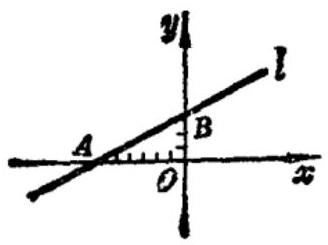
\includegraphics[max width=0.3\textwidth]{images/01912cc2-ffb6-728e-9ae7-b113ff05c64b_30_525610.jpg}
  %\documentclass[tikz, border=5pt]{standalone}
\begin{document}
	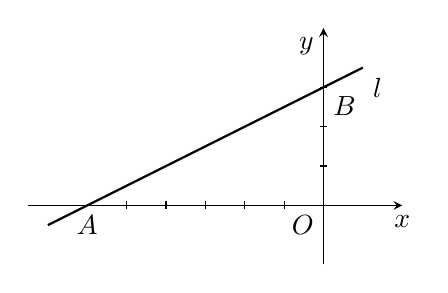
\begin{tikzpicture}[>=stealth, scale=0.5]
		% 绘制坐标轴
		\draw[->] (-7.5,0) -- (2,0) node[below] {$x$}; % x轴(带箭头和标签)
		\draw[->] (0,-1.5) -- (0,4.5) node[below left] {$y$}; % y轴(带箭头和标签)
		\node at (0,0) [below left] {$O$};           % 原点O的标签
		% 直线l  y=x/2+3
		\draw[thick] (-7, -0.5) -- (1, 3.5) node[below right] {$l$}; 
		% 绘制所有小刻度线(从 -1 到 2,每隔 1 单位画竖线)
		\foreach \x in {-5, -4,...,-1} {
			\draw (\x, 0.1) -- (\x, -0.1);  % 小竖线(长 0.2 单位)
		}
		\foreach \y in {0,1,...,3} {
			\draw (0.1,\y) -- (-0.1,\y);  % 小竖线(长 0.2 单位)
		}
		% 标记各点的标签 实心圆点
		%		\fill (G) circle (2pt) node [right] {$G$};  % 带标签的实心点
		\node at (-6,0) [below] {$A$}; 
		\node at (0,3) [below right] {$B$}; 
		
	\end{tikzpicture}
\end{document}

  \caption{图 1-23}
\end{figure}

画一条直线时, 只要找出这条直线上的任意两点就可以了. 通常是找出直线与两个坐标轴的交点. 上面已经求得直线 \(l\) 与 \(x\) 轴、 \(y\) 轴的交点:

\[
  A\left( {-6,0}\right) \text{、}B\left( {0,3}\right) \text{.}
\]

过点 \(A\text{、}B\) 作直线,就得直线 \(l\) (如图 1-23).

\begin{problemset}[练习]

\item 由下列各条件, 写出直线的方程, 并且化成一般式:

(1) 斜率是 \(- \frac{1}{2}\) ,经过点 \(A\left( {8, - 2}\right)\) ;

(2) 经过点 \(B\left( {4,2}\right)\) ,平行于 \(x\) 轴;

(3)经过点 \(C\left( {-\frac{1}{2},0}\right)\) ,平行于 \(y\) 轴;

(4)在 \(x\) 轴和 \(y\) 轴上的截距分别是 \(\frac{3}{2}\text{、} - 3\) ;

(5) 经过两点 \({P}_{1}\left( {3, - 2}\right) \text{、}{P}_{2}\left( {5, - 4}\right)\) ;

(6) \(x\) 轴上的截距是 -7,倾斜角是 \({45}^{ \circ }\) .

\item 已知直线 \({Ax} + {By} + C = 0\) ,

(1) 当 \(B \neq 0\) 时,斜率是多少? 当 \(B = 0\) 时呢?

(2) 系数为什么值时, 方程表示通过坐标原点的直线.

\item 求下列直线的斜率和在 \(y\) 轴上的截距,并画出图形:

(1) \({3x} + y - 5 = 0\) ; (2) \(\frac{x}{4} - \frac{y}{5} = 1\) ;

(3) \(x + {2y} = 0\) ; (4) \({7x} - {6y} + 4 = 0\) ;

(5) \({2y} - 7 = 0\) .

\end{problemset}

\section{*二元一次不等式表示的区域}

前面, 我们研究了二元一次方程和直线的关系, 用同样的方法, 也可以研究二元一次不等式和以它的解为坐标的点的集合 (图形) 的关系.

含有两个未知数, 并且未知数的次数都是一次的不等式叫做二元一次不等式. 使不等式成立的未知数的值叫做它的解.

我们研究不等式

\[
  y > {2x} + 1 \tag{1}
\]

的解, 并把它在坐标平面上表示出来.

为了求 (1) 式的任何一个实数解,可任意选取 \(x\) 的一个实数值,例如 \(x = 1\) ,把它看作一次方程,这个方程的图形是平行于 \(y\) 轴的直线,它与直线 \(l : y = {2x} + 1\) 相交于点 \(A\left( {1,3}\right)\) (图 1-24).

在直线 \(x = 1\) 上,点 \(A\) 上方的所有点,如 \(B\left( {1,4}\right) \text{、}C\left( {1,5}\right)\) 、 \(\cdots\) 的坐标都满足不等式 (1), 它们都是 (1) 式的解.

在直线 \(x = 1\) 上,点 \(A\) 下方的所有点,如 \({B}^{\prime }\left( {1,2}\right)\) 、 \({C}^{\prime }\left( {1,1}\right) \text{、}\cdots\) 的坐标都不满足不等式 \(\left( 1\right)\) ,它们都不是 \(\left( 1\right)\) 的解.

可见, 以不等式 (1) 的解为坐标的所有点的集合

\[
  P = \{ M \mid y > {2x} + 1\}
\]

\begin{figure}[h]
  \centering
%  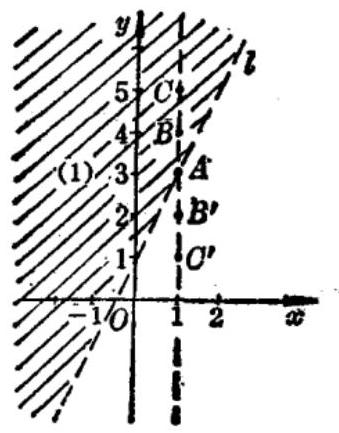
\includegraphics[max width=0.4\textwidth]{images/01912cc2-ffb6-728e-9ae7-b113ff05c64b_32_144093.jpg}
  %\documentclass[tikz, border=5pt]{standalone}
\usetikzlibrary{patterns} % 加载斜线阴影库
\begin{document}
	\begin{tikzpicture}[>=stealth, scale=1]
		
		% 5. 绘制阴影区域(东北斜线填充)位于最下层,
		\filldraw[pattern=north east lines, pattern color=gray!50] (-1.5,-2) -- (-2,-2) -- (-2,6) -- (2.5,6)  ;
		\draw[white]  (-1.5,-2) -- (-2,-2) -- (-2,6) -- (2.5,6);
		
		% 1. 绘制坐标轴
		\draw[->] (-2,0) -- (3,0) node[below] {$x$}; % x轴(带箭头和标签)
		\draw[->] (0,-2) -- (0,7) node[below left] {$y$}; % y轴(带箭头和标签)
		\node at (0,0) [below left] {$O$};          % 原点标记
		
		% 绘制所有小刻度线(从 -1 到 2,每隔 1 单位画竖线)
		\foreach \x in {-2, -1,...,2} {
			\ifnum\x=0 % 若x=0,则不绘制刻度
			\else % 否则绘制刻度线和标签
			\draw (\x, 0.1) -- (\x, -0.1) node[below] {$\x$};
			\fi
			
%			\draw (\x, 0.1) -- (\x, -0.1) node[below] {$\x$};  % 小竖线(长 0.2 单位)x轴刻度标记
		}
		\foreach \y in {1,2,...,6} {
			\draw (0.1,\y) -- (-0.1,\y) node[left] {$\y$};  % 小竖线(长 0.2 单位)y轴刻度标记
		}
		
		% 2. 绘制直线  l 虚线 y=2x+1 
		\draw[dashed , thick] (-1.5,-2) -- (2.5,6) node[below right] {$l$}; % 虚线部分
		
		% 3. 绘制竖直线 \( x=1 \)(虚线)
		\draw[dashed, thick ] (1,-2) -- (1,6);
		
		% 4. 标记各点(A、B、C、B'、C')
		\fill (1,3) circle (1pt) node [right] {$A$};
		\fill (1,4) circle (1pt) node [right] {$B$};
		\fill (1,5) circle (1pt) node [right] {$C$};
		\fill (1,2) circle (1pt) node [right] {$B'$};
		\fill (1,1) circle (1pt) node [right] {$C'$};
		
		\node at (-1,3) [left] {$(1)$};
		
	\end{tikzpicture}
\end{document}

  \caption{图 1-24}
\end{figure}

是直线 \(l\) 上方的半平面所有的点, 也就是图 1-24 中阴影所表示的平面部分, 但不包括边界直线. 这种情况,直线 \(l\) 在图中一般画成虚线.

以二元一次不等式的解为坐标的所有点的集合表示一个平面图形, 我们把这个图形叫做不等式表示的区域.

由上例知道, \(y > {2x} + 1\) 表示的区域是直线 \(l\) 上方的半平面; 同理,容易求得 \(y < {2x} + 1\) 表示的区域是直线 \(l\) 下方的半平面; 而 \(y = {2x} + 1\) 就是边界直线 \(l\) .

一般地, \(y = {kx} + b\) 的直线把平面分成两个半平面, \(y > {kx}\) \(+ b\) 表示的区域是直线上方的半平面; \(y < {kx} + b\) 表示的区域是直线下方的半平面; 直线 \(y = {kx} + b\) 是两个半平面的边界线.

例 1 画出不等式 \(y \leq - {2x} + 3\) 表示的区域.

解: 不等式 \(y \leq - {2x} + 3\) 的解集是

\[
  y = - {2x} + 3 \tag{1}
\]

\[
  y < - {2x} + 3 \tag{2}
\]

\begin{figure}[h]
  \centering
%  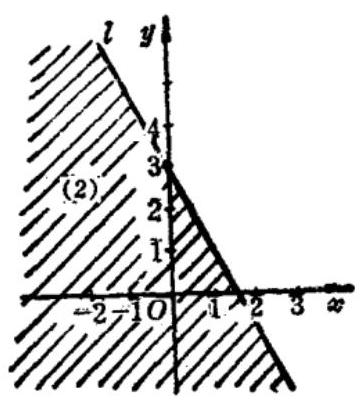
\includegraphics[max width=0.4\textwidth]{images/01912cc2-ffb6-728e-9ae7-b113ff05c64b_33_345679.jpg}
  %\documentclass[tikz, border=5pt]{standalone}
\usetikzlibrary{patterns} % 加载斜线阴影库
\begin{document}
	\begin{tikzpicture}[>=stealth, scale=1]
		
		% 4. 绘制阴影区域(东北斜线填充)位于最下层,
		\filldraw[pattern=north east lines, pattern color=gray!50] (2.5,-2) -- (-2.5,-2) -- (-2.5,6) -- (-1.5,6)  ;
		\draw[white]  (2.5,-2) -- (-2.5,-2) -- (-2.5,6) -- (-1.5,6);
		
		% 1. 绘制坐标轴
		\draw[->] (-3,0) -- (3.5,0) node[below] {$x$}; % x轴(带箭头和标签)
		\draw[->] (0,-2.2) -- (0,6.5) node[below left] {$y$}; % y轴(带箭头和标签)
		\node at (0,0) [below left] {$O$};          % 原点标记
		
		% 绘制所有小刻度线(从 -1 到 2,每隔 1 单位画竖线)
		\foreach \x in {-2, -1,...,3} {
			\ifnum\x=0 % 若x=0,则不绘制刻度
			\else % 否则绘制刻度线和标签
			\draw (\x, 0.1) -- (\x, -0.1) node[below] {$\x$};
			\fi
		}
			
%			\draw (\x, 0.1) -- (\x, -0.1) node[below] {$\x$};  % 小竖线(长 0.2 单位)x轴刻度标记
%		}
		\foreach \y in {1,2,...,5} {
			\draw (0.1,\y) -- (-0.1,\y) node[left] {$\y$};  % 小竖线(长 0.2 单位)y轴刻度标记
		}
		
		% 2. 绘制直线  l 虚线 y=-2x+3 
		\draw[thick] (2.5,-2) -- (-1.5, 6) node[ right] {$l$}; % 虚线部分
		
		% 3. 标记各点(A、B、C、B'、C')
		\fill (0,3) circle (1pt) ;
		
		\node at (-1,2) [left] {$(2)$};
		
	\end{tikzpicture}
\end{document}

  \caption{图 1-25}
\end{figure}

的解集的并集, 所以它们表示的区域是由 (1)、(2) 的图形合成的.

因为 (1) 式的图形是直线 \(l\) ; (2) 式的图形是直线 \(l\) 下方的半平面. 所以已知不等式表示的区域是直线 \(l\) 和它下方的半平面,也就是图 1-25 阴影部分并且包括直线. 这种情况,直线 \(l\) 在图中一般画成实线.

由上面的讨论容易想到, 一般二元一次不等式

\[
    {Ax} + {By} + C > 0
\]

表示的区域,一定是在直线 \({Ax} + {By} + C = 0\) 的某一侧. 但要断定究竟是在哪一侧,并不需要将不等式化为 \(y\) 的函数式,可以取直线 \({Ax} + {By} + C = 0\) 一侧的一点,将它的坐标代入不等式, 如果不等式成立, 那么这一侧就是不等式表示的区域; 如果不等式不成立, 那么直线的另一侧是不等式表示的区域.

除选点代入不等式的方法外,也可以用 \(y\) 的系数判断不等式表示的区域. 如果 \(B > 0\) (或 \(B < 0\) ),那么不等式 \({Ax} + {By}\) \(+ C > 0\) 所表示的区域是直线 \({Ax} + {By} + C = 0\) 的上 (或下) 方的半平面; 如果不等式写成 \({Ax} + {By} + C < 0\) 的形式时,它表示的区域是直线下 (或上) 方的半平面. 想一想,如果 \(B = 0\) 时, 原不等式表示什么样的区域.

例 2 求不等式

\[
  x + {2y} - {10} < 0 \tag{1}
\]

表示的区域, 并画出图形.

解: 先画出直线 \(l : x + {2y} - {10} = 0\) .

用选点代入不等式 \(\left( 1\right)\) 的方法,例如将原点 \(\left( {0,0}\right)\) 的坐标

代入 \(\left( 1\right)\) 式,得 \(- {10} < 0,\left( 1\right)\) 式成立. 所以坐标原点所在的半平面是不等式 (1) 表示的区域, 即直线 \(l\) 下方的半平面,如图 1-26 的阴影部分, 但不包括直线 \(l\) .

\begin{figure}[h]
  \centering
%  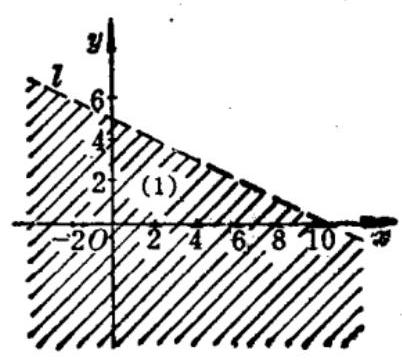
\includegraphics[max width=0.4\textwidth]{images/01912cc2-ffb6-728e-9ae7-b113ff05c64b_34_186358.jpg}
  %\documentclass[tikz, border=5pt]{standalone}
\usetikzlibrary{patterns} % 加载斜线阴影库
\begin{document}
	\begin{tikzpicture}[>=stealth, scale=0.6]
		
		% 4. 绘制阴影区域(东北斜线填充)位于最下层,
		\filldraw[pattern=north east lines, pattern color=gray!50] (-2.5, 6.25) -- (-2.5,-1.5) -- (11,-1.5) -- (11,-0.5)  ;
		\draw[white] (-2.5, 6.25) -- (-2.5,-1.5) -- (11,-1.5) -- (11,-0.5) ;
		
		% 1. 绘制坐标轴
		\draw[->] (-3,0) -- (11.5,0) node[below] {$x$}; % x轴(带箭头和标签)
		\draw[->] (0,-2) -- (0,7.5) node[below left] {$y$}; % y轴(带箭头和标签)
		\node at (0,0) [below left] {$O$};          % 原点标记
		
		% 绘制所有小刻度线(从 -1 到 2,每隔 1 单位画竖线)
		% 遍历x值,排除0刻度
		\foreach \x in {-2, 0,...,10} {
			\ifnum\x=0 % 若x=0,则不绘制刻度
			\else % 否则绘制刻度线和标签
			\draw (\x, 0.1) -- (\x, -0.1) node[below] {$\x$};
			\fi
		}
		
%		\foreach \x in {-2, 0,...,10} {
%			\draw (\x, 0.1) -- (\x, -0.1) node[below] {$\x$};  % 小竖线(长 0.2 单位)x轴刻度标记
%		}

		\foreach \y in {2,4,...,6} {
			\draw (0.1,\y) -- (-0.1,\y) node[left] {$\y$};  % 小竖线(长 0.2 单位)y轴刻度标记
		}
		
		% 2. 绘制直线  l 虚线 y=-x/2+5 
		\draw[dashed , thick] (11,-0.5) -- (-2.5, 6.25) node[ right] {$l$}; % 虚线部分
		
		% 3. 标记各点(A、B、C、B'、C')
		\fill (0,5) circle (1pt) ;
		
		\node at (2,2) [left] {$(1)$};
		
	\end{tikzpicture}
\end{document}

  \caption{图 1-26}
\end{figure}

例 2 也可以用如下解法:

解: 用 \(y\) 的系数判断不等式 (1) 表示的区域.

\(\because \;B = 2 > 0\) ,

\(\therefore x + {2y} - {10} < 0\) 表示的区域是直线 \(x + {2y} - {10} = 0\) 下方的半平面, 但不包括直线.

例 3 某工厂有一批长为 2.5 米的条形钢材, 要截成 60 厘米和 42 厘米两种规格的零件毛坯, 找出最佳的下料方案并计算材料的利用率.

解: 设每根钢材可截成 60 厘米长的毛坯 \(x\) 根和 42 厘米长的毛坯 \(y\) 根. 按题意得不等式

\[
    {0.6x} + {0.42y} \leq {2.5}\text{.} \tag{1}
\]

在坐标纸上画出

\[
    {0.6x} + {0.42y} = {2.5} \tag{2}
\]

的直线. 如图 1-27.

\begin{figure}[h]
  \centering
%  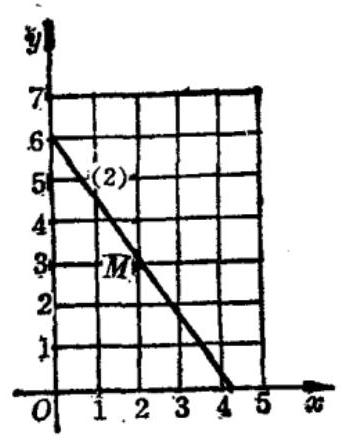
\includegraphics[max width=0.4\textwidth]{images/01912cc2-ffb6-728e-9ae7-b113ff05c64b_35_684997.jpg}
  %\documentclass[tikz, border=5pt]{standalone}
\begin{document}
	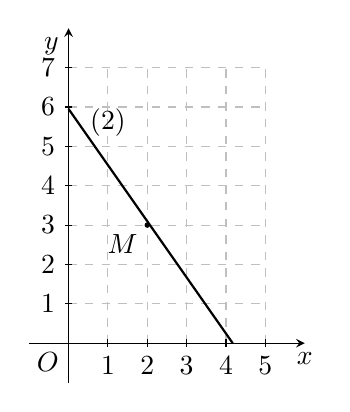
\begin{tikzpicture}[>=stealth, scale=0.5]
		% 1. 绘制坐标轴
		\draw[->] (-1,0) -- (6,0) node[below ] {$x$};  % x轴(带箭头和标签)
		\draw[->] (0,-1) -- (0,8) node[below left] {$y$};  % y轴(带箭头和标签)
		\node at (0,0) [below left] {$O$};           % 原点标记
		
		% 2. 绘制网格线(虚线)
		\foreach \x in {1,2,...,5} {
			\draw[dashed, gray!50] (\x,0) -- (\x,7);  % 垂直网格线
			\draw (\x, 0.1) -- (\x, -0.1) node[below] {$\x$};  % 小竖线(长 0.2 单位)x轴刻度标记
		}
		\foreach \y in {1,2,...,7} {
			\draw[dashed, gray!50] (0,\y) -- (5,\y);  % 水平网格线
			\draw (0.1,\y) -- (-0.1,\y) node[left] {$\y$};  % 小竖线(长 0.2 单位)y轴刻度标记
		}
		
		% 3. 绘制直线(从 (0,6) 到 (4,0))
		\draw[thick] (0,5.95) -- (4.17,0);
		
		% 4. 标记点 M(2,3)
		\fill (2,3) circle (2pt);           % 绘制点 M
		\node at (2,3) [below left] {$M$}; % 标注点 M
		
		% 5. 标注区域 (2)
		\node at (1,5) [ above] {(2)};
		
	\end{tikzpicture}
\end{document}

  \caption{图 1-27}
\end{figure}

因为要截得的两种毛坯数的和必须是正整数, 所以以 (1) 的解为坐标的点一定是第一象限内的网格的交点.

如果直线 (2) 上有网格的交点, 那么按直线上网格交点的坐标 \(\left( {x,y}\right)\) 的值作为下料方案, 这时材料全被利用, 因此这个方案就是最佳方案. 但从图 1-27 中可以看出, 直线 (2) 不通过网格交点, 在这种情况下, 为了制订最佳下料方案, 应该找靠近直线 (2) 的网格交点.

当然不能在直线(2)的上方半平面内找网格交点. 因为 \(B = {0.42} > 0\) ,上方半平面内任何网格交点的坐标都使 \({0.6x}\) \(+ {0.42y} > {2.5}\) ,这时两种零件毛坯长度的和超过了原钢材长, 这是不合理的.

这样,下料范围只能限制在 \({0.6x} + {0.42y} < {2.5}\) 表示的区, 域内. 这个区域是直线(2)下方的半平面. 在直线(2)的下方半平面上找到最靠近直线的网格交点,得点 \(M\left( {2,3}\right)\) .

\(x = 2,y = 3\) 就是所求的解,按这样截取毛坯,材料尽管没有被完全利用, 但废料最少.

材料的利用率

\[
  \frac{{0.6} \times 2 + {0.42} \times 3}{2.5} = {98.4}\% \text{.}
\]

答: 把每根条钢截成 2 根 60 厘米长和 3 根 42 厘米长的零件毛坯是最佳的下料方案. 材料利用率为 \({98.4}\%\) .

\begin{problemset}[练习]

\item 求下列不等式表示的区域:

(1) \(y < - {2x} - 1\) ; (2) \(y \geq - x + 3\) ; (3) \(x + {2y} - 5 < 0\) ;

(4) \({5x} - {3y} + 2 \geq 0\) ; (5) \(x \geq 4\) ; (6) \(y \leq - 3\) ;

(7) \(y \leq {3x}\) ; (8) \(x \leq - {2y}\) ; (9) \({3x} + {2y} < 0\) .

\item 已知 \(y < {kx} + b\) 表示直线 \(y = {kx} + b\) 下方的半平面,说明当 \(B < 0\) 时,不等式 \({Ax} + {By} + C > 0\) 表示的区域是直 线 \({Ax} + {By} + C = 0\) 下方的半平面.

\item 已知每袋面粉 50 斤, 每袋大米 210 斤, 用栽重量是 530 斤的小推车运输, 找出车运效率最高的装车方案.

\end{problemset}

\section{* 直线型经验公式}

在生产和科学实验中, 常常需要根据观察或实验所得的两个变量的一些对应的近似值 (叫做实验数据), 来求出这两个变量之间的函数关系的解析式. 这样通过实验数据得到的两个变量的关系式叫做经验公式. 如果所求得的经验公式是一次方程, 它就叫做直线型经验公式.

下面举例说明求直线型经验公式的方法.

例 通过实验,测得某种合金的熔点 \(y\left( {{}^{ \circ }\mathrm{C}}\right)\) 和含铅量 \(x\left( \% \right)\) 之间关系的数据如下表:

\begin{center}
  \adjustbox{max width=\textwidth}{
    \begin{tabular}{|c|c|c|c|c|c|c|}
      \hline
      \(x\left( \% \right)\) & 36.9 & 46.7 & 63.7 & 77.8 & 84.0 & 87.5 \\
      \hline
      \(y\left( {{}^{ \circ }\mathrm{C}}\right)\) & 181 & 197 & 235 & 270 & 283 & 292 \\
      \hline
    \end{tabular}
  }
\end{center}

根据这些数据,求关于 \(x\text{、}y\) 的经验公式.

解: (1) 把各组对应的数据作为点的坐标, 在坐标平面上画出这些点. 例如,以 \(\left( {{63.7},{235}}\right)\) 为坐标的点就是 \(P\) (图 1-28).

(2)观察这些点的位置, 可以看出它们大致分布在一条直线上. 用透明尺的边缘在这些点间移动, 使它尽量靠近或通过大多数点, 然后画出直线.

(3)求方程: 在这条直线上选出两点,例如 \(A({46.7}\) , 197)、 \(B\left( {{84.0},{283}}\right)\) 、把它们的坐标代入直线的两点式方程, 得

\[
  \frac{y - {197}}{{283} - {197}} = \frac{x - {46.7}}{{84.0} - {46.7}}
\]

\begin{figure}[h]
  \centering
%  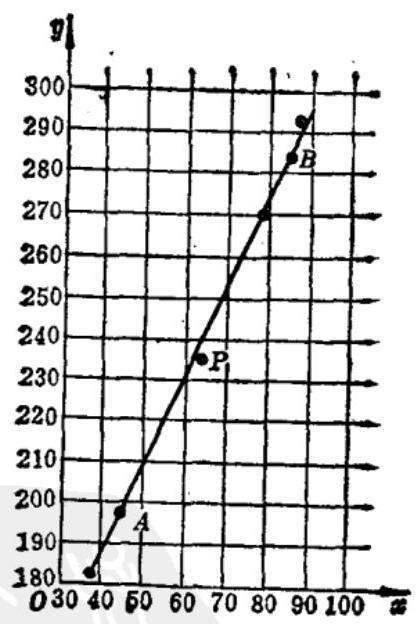
\includegraphics[max width=0.4\textwidth]{images/01912cc2-ffb6-728e-9ae7-b113ff05c64b_37_976668.jpg}
  %\documentclass[tikz, border=5pt]{standalone}
\begin{document}
	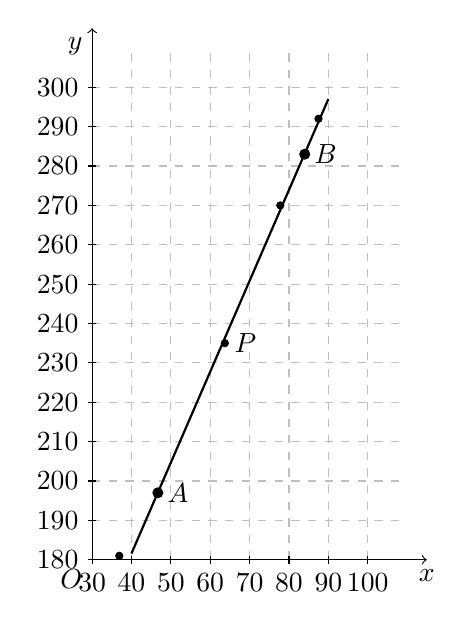
\begin{tikzpicture}[scale=0.5]
		% 2. 绘制网格线(虚线)
		\foreach \x in {0,1,2,...,7} {
			\draw[dashed, gray!50] (\x,0) -- (\x,13);  % 垂直网格线
			% 计算 \x * 10 + 30 并存储到 \result(整数)
			\pgfmathtruncatemacro{\result}{\x * 10 + 30}
			% 绘制刻度短线 + 标注计算后的值
			\draw (\x, 0.1) -- (\x, -0.1) node[below] {$\result$};  % 小竖线(长 0.2 单位)x轴刻度标记 =10x+30
		}
		\foreach \y in {0,1,2,...,12} {
			\draw[dashed, gray!50] (0,\y) -- (8,\y);  % 水平网格线
			\pgfmathtruncatemacro{\result}{\y * 10 + 180}
			\draw (0.1,\y) -- (-0.1,\y) node[left] {$\result$};  % 小竖线(长 0.2 单位)y轴刻度标记
		}
		
		
		% 1. 绘制坐标轴
		\draw[->] (0, 0) -- (8.5, 0) node[below ] {$x$};  % x轴(带箭头和标签)
		\draw[->] (0, 0) -- (0, 13.5) node[below left] {$y$};  % y轴(带箭头和标签)
		\node at (0,0) [below left] {$O$};           % 原点标记
%		\node at (0,0) [below ] {$30$}; 
%		\node at (0,0) [ left] {$180$}; 
		
		
		% 3. 绘制直线(从 (1,0.16) 到 (6,11.7))
		\draw[thick] (1,0.16) -- (6,11.7);
		
		% 4. 标记点 (近似)y≈2.31x−21.5  A(16.7,17) 和 B(54,103)
		\fill (1.67,1.7) circle (4pt) node [ right] {$A$};  % 绘制标注点 A
		\fill (5.4,10.3) circle (4pt) node [ right] {$B$};  % 绘制标注点 B
		\fill (0.69,0.1) circle (3pt) ; 
		\fill (3.37,5.5) circle (3pt) node [ right] {$P$};  % 绘制标注点 P
		\fill (4.78,9) circle (3pt) ;  % 绘制标注点 
		\fill (5.75,11.2) circle (3pt) ;  % 绘制标注点 
		
	\end{tikzpicture}
\end{document}

  \caption{图 1-28}
\end{figure}

化简后, 就得经验公式

\[
  y = {2.3x} + {89.3}\text{. }
\]

有了这个经验公式, 就可以从这种合金的含铅量求得对应的熔点, 或者反过来, 从这种合金的熔点求得对应的含铅量.

上面这种选择两点求直线型经验公式的方法, 叫做选点法.

选点法虽然比较简便, 但是由于选点的灵活性较大, 一般精确度不高. 下面再介绍一种精确度较高的方法, 叫做平均值法.

我们仍用上面的例题来说明平均值法. 在确定经验公式是直线型的以后, 可假定所求的经验公式为

\[
  y = {kx} + b.
\]

把表中 \(x\text{、}y\) 的对应值代入这个方程,得到若干个关于 \(k\) 、 \(b\) 的一次方程. 为了确定 \(k\text{、}b\) 的值,把它们分成两组,使两组中的方程个数相同或相差一个, 再把各组方程两边分别相加, 就得到关于 \(k\text{、}b\) 的两个方程:

\[
  \begin{aligned} {181} & = {36.9k} + b & {270} & = {77.8k} + b \\ {197} & = {46.7k} + b & {283} & = {84.0k} + b \\ + ){235} & = {63.7k} + b & + ){292} & = {87.5k} + b \\ {613} & = {147.3k} + {3b} & {845} & = {249.3k} + {3b} \end{aligned}
\]

解方程组

\[
  \left\{ \begin{array}{l} {613} = {147.3k} + {3b} \\ {845} = {249.3k} + {3b} \end{array}\right.
\]

得

\[
  k \approx {2.27},\;b \approx {92.9}.
\]

代入所设方程, 就得到所求的经验公式

\[
  y = {2.27x} + {92.9}.
\]

\begin{problemset}[练习]

\item 丙烯腈是合成人造羊毛的原料. 在研究它的比重 \(D\) 和温度 \(T\left( {{}^{ \circ }\mathrm{C}}\right)\) 的关系时,通过实验得到的数据如下:

\begin{center}
  \adjustbox{max width=\textwidth}{
    \begin{tabular}{|c|c|c|c|c|c|c|c|}
      \hline
      \(T\left( {{}^{ \circ }\mathrm{C}}\right)\) & 0 & 5 & 10 & 15 & 20 & 25 & 30 \\
      \hline
      D & 0.8287 & 0.8282 & 0.8276 & 0.8271 & 0.8266 & 0.8261 & 0.8255 \\
      \hline
    \end{tabular}
  }
\end{center}

用选点法求出 \(D\) 与 \(T\) 之间的经验公式.

\item 根据下列实验数据,用平均值法求关于 \(m\text{、}p\) 的经验公式:

\begin{center}
  \adjustbox{max width=\textwidth}{
    \begin{tabular}{|c|c|c|c|c|c|c|c|}
      \hline
      \(m\) & 0.03 & 0.05 & 0.10 & 0.14 & 0.17 & 0.20 & 0.25 \\
      \hline
      \(p\) & 0 & 0.42 & 0.93 & 1.60 & 2.08 & 2. 41 & 3. 31 \\
      \hline
    \end{tabular}
  }
\end{center}

\end{problemset}

\begin{problemset}[习 题 二]

\item 四边形 \({ABCD}\) 的四个顶点是 \(A\left( {2,3}\right) \text{、}B\left( {1, - 1}\right) \text{、}C( - 1\) , \(- 2)\text{、}D\left( {-2,2}\right)\) . 求四边所在直线的倾斜角和斜率.

\item 根据下列条件写出直线的方程:

(1)斜率是 \(\frac{\sqrt{3}}{3}\) ,经过点 \(A\left( {8, - 2}\right)\) ;

(2)过点 \(B\left( {-2,0}\right)\) ,且与 \(x\) 轴垂直;

(3)斜率为 -4,在 \(y\) 轴上的截距为 7 ;

(4)经过两点 \(A\left( {-1,8}\right) \text{、}B\left( {4, - 2}\right)\) ;

(5) 在 \(y\) 轴上的截距是 2,且与 \(x\) 轴平行;

(6) 在 \(x\) 轴、 \(y\) 轴上的截距分别是 4 与 -3 .


\item 已知直线的斜率 \(k = 2,{P}_{1}\left( {3,5}\right) \text{、}{P}_{2}\left( {{x}_{2},7}\right) \text{、}{P}_{3}\left( {-1,{y}_{3}}\right)\) 是这条直线上的三个点. 求 \({x}_{2}\) 和 \({y}_{8}\) .

\item 已知两点 \(M\left( {2,2}\right)\) 和 \(N\left( {5, - 2}\right)\) ,点 \(P\) 在 \(x\) 轴上,且 \(\angle {MPN} = {Rt}\angle\) . 求点 \(P\) 的坐标.

\item 设 \(A\text{、}B\) 两点的坐标分别是 \(\left( {{x}_{1},{y}_{1}}\right)\) 和 \(\left( {{x}_{2},{y}_{2}}\right)\) ,直线 \({AB}\) 的倾斜角是 \(\alpha\) . 求证:

\[
  \left| {{x}_{1} - {x}_{2}}\right| = \sqrt{{\left( {x}_{2} - {x}_{1}\right) }^{2} + {\left( {y}_{2} - {y}_{1}\right) }^{2}}\left| {\cos \alpha }\right| .
\]

\item 一条直线经过点 \(A\left( {2, - 3}\right)\) ,它的倾斜角等于直线 \(y = \frac{1}{\sqrt{3}}x\) 的倾斜角的 2 倍,求这条直线的方程.

\item 一根弹簧, 挂 4 公斤的物体时, 长 20 厘米, 在弹性限度内, 所挂物体的重量每增加 1 公斤, 弹簧伸长 1.5 厘米. 利用点斜式写出弹簧的长度 \(l\) (厘米) 和所挂物体重量 \(\mathbf{F}\) (公斤) 之间关系的方程.

\item 一条直线和 \(y\) 轴相交于点 \(P\left( {0,2}\right)\) ,它的倾斜角的正弦是 \(\frac{4}{5}\) . 求这条直线的方程. 这样的直线有几条?

\item 证明: 三点 \(A\left( {1,3}\right) \text{、}B\left( {5,7}\right) \text{、}C\left( {{10},{12}}\right)\) 在同一条直线上.

\item (1) 已知三角形的顶点是 \(A\left( {8,5}\right) \text{、}B\left( {4, - 2}\right) \text{、}C\left( {-6,3}\right)\) , 求经过每两边中点的三条直线的方程.

(2) \(\bigtriangleup {ABC}\) 的顶点是 \(A\left( {0,5}\right) \text{、}B\left( {1, - 2}\right) \text{、}C\left( {-6,4}\right)\) , 求 \({BC}\) 边上的中线所在直线的方程.

\item 一根铁棒在 \({40}^{ \circ }\mathrm{C}\) 时长 12.506 米,在 \({80}^{ \circ }\mathrm{C}\) 时长 12.512 米, 已知长度 \(l\) (米) 和温度 \(t\left( {{}^{ \circ }\mathrm{C}}\right)\) 的关系可以用直线方程来表示, 用两点式表示这个方程, 并且根据这个方程, 求这根铁棒在 \({100}^{ \circ }\mathrm{C}\) 时的长度.

\item 菱形的两条对角线长分别等于 8 和 6,并且分别放置在 \(x\) 轴和 \(y\) 轴上. 求菱形各边所在的直线的方程.

\item 求过点 \(P\left( {2,3}\right)\) ,并且在两轴上的截距相等的直线方程.

\item 油槽储油 20 立方米, 从一管道等速流出, 50 分钟流 完. 用截距式写出关于油槽里剩余的油量 \(Q\) (立方米) 和流出的时间 \(t\) (分) 的方程,并且画出图形 (注意: \(0 \leq t \leq {50}\) ).

\item 直线方程 \({Ax} + {By} + C = 0\) 的系数 \(A\text{、}B\text{、}C\) 满足什么关系时,这条直线 (1) 与坐标轴都相交; (2) 只与 \(x\) 轴相交; (3)只与 \(y\) 轴相交; (4) 是 \(x\) 轴; (5) 是 \(y\) 轴.

\item 设点 \(P\left( {{x}_{0},{y}_{0}}\right)\) 在直线 \({Ax} + {By} + C = 0\) 上. 求证: 这条直线的方程可以写成 \(A\left( {x - {x}_{0}}\right) + B\left( {y - {y}_{0}}\right) = 0\) .

\item * 求下列不等式表示的区域:

(1) \(y \geq x\) ; (2) \(x < {2y}\) ;

(3) \({3y} \leq {2x}\) ; (4) \({3y} - 2 \leq 0\) ;

(5) \({3x} - {5y} + {10} > 0\) ; (6) \({2x} + {3y} - 4 \geq 0\) .

\item * 某同学拿 5 元钱买纪念邮票, 票面 4 分钱的每套 5 张, 8 分钱的每套 4 张. 如果每种至少买一套, 共有几种买法, 能否恰好将钱用完, 怎样买剩钱最少?

\item * 有一滑轮组,举起的物重 \(W\) 与需用的力 \(F\) 之间的关系,由实验所得的数据如下表:

\begin{center}
  \adjustbox{max width=\textwidth}{
    \begin{tabular}{|c|c|c|c|c|c|}
      \hline
      \(W\) (公斤) & 20 & 40 & 60 & 80 & 100 \\
      \hline
      \(F\) (公斤) & 4. 35 & 7. 55 & 10.40 & 13.80 & 16.80 \\
      \hline
    \end{tabular}
  }
\end{center}

求适合以上关系的直线型经验公式.

\item * 一个弹簧的长度 \(l\) 和它悬挂的重量 \(W\) 间关系的实验数据如下:

\begin{center}
  \adjustbox{max width=\textwidth}{
    \begin{tabular}{|c|c|c|c|c|c|c|}
      \hline
      \(W\) & 2 & 4 & 6 & 8 & 10 & 12 \\
      \hline
      \(l\) & 8.9 & 10.1 & 11.2 & 12.0 & 13. 1 & 13.9 \\
      \hline
    \end{tabular}
  }
\end{center}

分别用选点法和平均值法求关于 \(l\text{、}W\) 的经验公式,并算出当 \(l = {9.2}\) 时, \(W\) 的值.

\end{problemset}

\section*{三 \text{ }两条直线的位置关系}

\section{两条直线的平行与垂直}

在平面几何中, 我们研究过平面上两条直线互相平行或垂直的位置关系. 现在我们研究怎样通过直线的方程来判定两条直线平行或垂直.

设直线 \({l}_{1}\) 和 \({l}_{2}\) 的斜率为 \({k}_{1}\) 和 \({k}_{2}\) ,它们的方程分别是

\[
    {l}_{1} : y = {k}_{1}x + {b}_{1};\;{l}_{2} : y = {k}_{2}x + {b}_{2}.
\]

我们首先研究两条直线平行 (不重合) 的情形.

如果 \({l}_{1}//{l}_{2}\) (图 1-29),那么它们的倾斜角相等, \({\alpha }_{1} = {\alpha }_{2}\) .

\(\therefore\)

\[
  \operatorname{tg}{\alpha }_{1} = \operatorname{tg}{\alpha }_{2}
\]

即

\[
    {k}_{1} = {k}_{2}\text{.}
\]

反过来,如果两条直线的斜率相等, \({k}_{1} = {k}_{2}\) ,也就是 \(\operatorname{tg}{\alpha }_{1}\) \(= \operatorname{tg}{\alpha }_{2}\) .

\begin{figure}[h]
  \centering
%  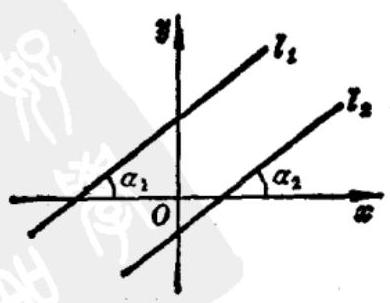
\includegraphics[max width=0.4\textwidth]{images/01912cc2-ffb6-728e-9ae7-b113ff05c64b_42_859750.jpg}
  %\documentclass[tikz, border=5pt]{standalone}
\usetikzlibrary{angles, quotes, shapes.geometric} % 加载角度、引用、直角标记库
\begin{document}
	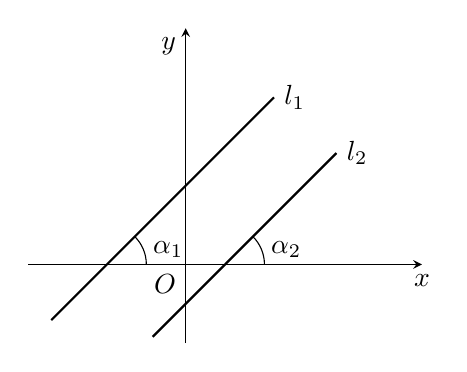
\begin{tikzpicture}[>=stealth, scale=1]
		% 1. 绘制坐标轴
		\draw[->] (-2,0) -- (3,0) node[below] {$x$}; % x轴(带箭头和标签)
		\draw[->] (0,-1) -- (0,3) node[below left] {$y$}; % y轴(带箭头和标签)
		\node at (0,0) [below left] {$O$}; % 原点标记
		
		% 2. 绘制直线 \( l_1 \)(倾斜向上)
		\draw[thick] (-1, 0) --  ++(45: 3) node[right] {$l_1$};
		\draw[thick] (-1, 0) --  ++(-135: 1) ;
		
		% 3. 绘制直线 \( l_2 \)(倾斜向下,与 \( l_1 \) 垂直)
		\draw[thick] (0.5, 0) -- ++(45: 2) node[right] {$l_2$};
		\draw[thick] (0.5, 0) -- ++(-135: 1.3) ;
		
		% 4. 标记角度 \( \alpha_1 \)(\( l_1 \) 与 x 轴正方向的锐角)
		\draw (-0.5, 0) arc (0:45:0.5) node[midway, right ] {$\alpha_1$};
		
		% 5. 标记角度 \( \alpha_2 \)(\( l_2 \) 与 x 轴正方向的角)
		\draw (1, 0) arc (0:45:0.5) node[midway, right ] {$\alpha_2$}; 
		
	\end{tikzpicture}
\end{document}

  \caption{图 1-29}
\end{figure}

由于 \({0}^{ \circ } \leq {\alpha }_{1} < {180}^{ \circ }\) ,

\[
    {0}^{ \circ } \leq {\alpha }_{2} < {180}^{ \circ }
\]

\(\therefore \;{\alpha }_{1} = {\alpha }_{2}\) .

又因为两条直线不重合,

\(\therefore {l}_{1}//{l}_{2}\) .
\begin{corollary}
两条直线有斜率且不重合, 如果它们平行, 则斜率相等; 反之, 如果它们的斜率相等, 则它们平行. 即

\[
    {l}_{1}//{l}_{2} \Leftrightarrow {k}_{1} = {k}_{2}\text{.}
\]

\end{corollary}

\textbf{geezhu:两条直线没有斜率且不重合,亦平行。}

例 1 已知两条不重合的直线

\[
    {l}_{1} : {2x} - {4y} + 7 = 0,\;{l}_{2} : x - {2y} + 5 = 0.
\]

求证: \({l}_{1}//{l}_{2}\) .

证明: 把 \({l}_{1}\text{、}{l}_{2}\) 的方程写成斜截式:

\[
    {l}_{1} : y = \frac{1}{2}x + \frac{7}{4},\;{l}_{2} : y = \frac{1}{2}x + \frac{5}{2}.
\]

则 \({l}_{1}\) 的斜率 \({k}_{1} = \frac{1}{2},\;{l}_{2}\) 的斜率 \({k}_{2} = \frac{1}{2}\) ,

\[
  \therefore \;{k}_{1} = {k}_{2}\text{. }
\]

又 \(\because\) 两条直线不重合,

\[
  \therefore \;{l}_{1}//{l}_{2}\text{. }
\]

例 2 求过点 \(A\left( {1, - 4}\right)\) ,且与直线 \({2x} + {3y} + 5 = 0\) 平行的直线方程.

解: 已知直线的斜率是 \(- \frac{2}{3}\) ,因为所求直线与已知直线

平行,因此它的斜率也是 \(- \frac{2}{3}\) .

根据点斜式, 得到所求直线的方程是

\[
  y + 4 = - \frac{2}{3}\left( {x - 1}\right)
\]

即

\[
    {2x} + {3y} + {10} = 0\text{. }
\]

现在研究两条直线垂直的情形.

如果 \({l}_{1} \bot {l}_{2}\) ,这时 \({\alpha }_{1} \neq {\alpha }_{2}\) ,(为什么?)

设 \({\alpha }_{2} < {\alpha }_{1}\) (图 1-30). 根据三角形外角等于和它不相邻的两内角的和, 得

\[
    {\alpha }_{1} = {90}^{ \circ } + {\alpha }_{2}
\]

\begin{figure}[h]
	\centering
	% 左侧图片:宽度设置为0.45倍文本宽度,预留间距
	\begin{subfigure}[h]{0.45\textwidth}
		\centering
%  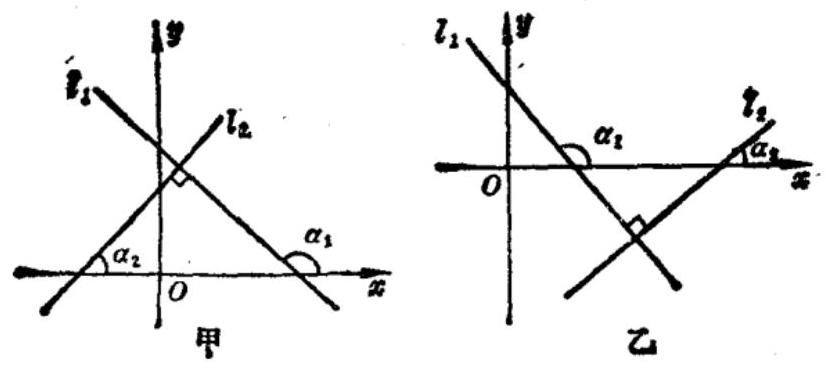
\includegraphics[max width=0.9\textwidth]{images/01912cc2-ffb6-728e-9ae7-b113ff05c64b_44_991124.jpg}
		%\documentclass[tikz, border=5pt]{standalone}
\usetikzlibrary{angles, quotes, shapes.geometric} % 加载角度、引用、直角标记库
\begin{document}
	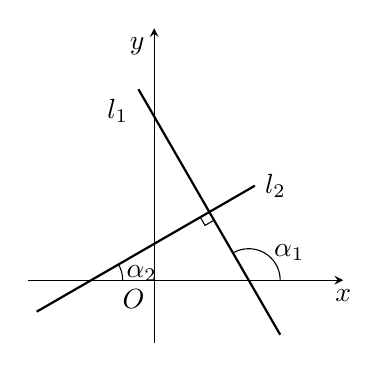
\begin{tikzpicture}[>=stealth, scale=0.8]
		
		% 1. 绘制坐标轴
		\draw[->] (-2,0) -- (3,0) node[below] {$x$}; % x轴(带箭头和标签)
		\draw[->] (0,-1) -- (0,4) node[below left] {$y$}; % y轴(带箭头和标签)
		\node at (0,0) [below left] {$O$}; % 原点标记
		
		% 2. 绘制直线 \( l_1 \)(倾斜向上)
		\draw[thick] (-1, 0) --  ++(30: 3) node[right] {$l_2$};
		\draw[thick] (-1, 0) --  ++(-150: 1) ;
		
		% 3. 绘制直线 \( l_2 \)(倾斜向下,与 \( l_1 \) 垂直)
		\draw[thick] (1.5, 0) -- ++(120: 3.5) node[below left] {$l_1$};
		\draw[thick] (1.5, 0) -- ++(-60: 1) ;
		
		% 4. 标记角度 \( \alpha_1 \)(\( l_1 \) 与 x 轴正方向的锐角)
		\draw (-0.5, 0) arc (0:30:0.5) ;
		\node at (-0.2, 0.1) []  {$\alpha_2$}; 
		
		% 5. 标记角度 \( \alpha_2 \)(\( l_2 \) 与 x 轴正方向的钝角)
		\draw (2, 0) arc (0:120:0.5) node[midway, right] {$\alpha_1$}; 
		
		% 6. 绘制直角标记(两直线垂直的符号)
		\draw (-1, 0) --  ++(30: 2) -- ++(-60: 0.15) -- ++(30: 0.15) ;
		
	\end{tikzpicture}
\end{document}

		\caption{甲}
	\end{subfigure}
	\hfill % 两个图片之间添加空白填充,确保左右分布
	% 右侧图片:宽度设置为0.45倍文本宽度
	\begin{subfigure}[h]{0.45\textwidth}
		\centering
		%\documentclass[tikz, border=5pt]{standalone}
\usetikzlibrary{angles, quotes, shapes.geometric} % 加载角度、引用、直角标记库
\begin{document}
	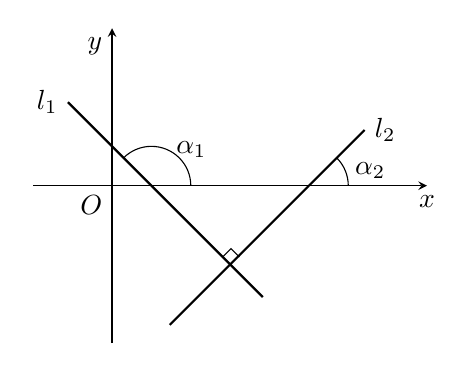
\begin{tikzpicture}[>=stealth, scale=1]
		
		% 1. 绘制坐标轴
		\draw[->] (-1,0) -- (4,0) node[below] {$x$}; % x轴(带箭头和标签)
		\draw[->] (0,-2) -- (0,2) node[below left] {$y$}; % y轴(带箭头和标签)
		\node at (0,0) [below left] {$O$}; % 原点标记
		
		% 2. 绘制直线 \( l_1 \)(倾斜向上)
		\draw[thick] (2.5, 0) --  ++(45: 1) node[right] {$l_2$};
		\draw[thick] (2.5, 0) --  ++(-135: 2.5) ;
		
		% 3. 绘制直线 \( l_2 \)(倾斜向下,与 \( l_1 \) 垂直)
		\draw[thick] (0.5, 0) -- ++(135: 1.5) node[ left] {$l_1$};
		\draw[thick] (0.5, 0) -- ++(-45: 2) ;
		
		% 4. 标记角度 \( \alpha_1 \)(\( l_1 \) 与 x 轴正方向的锐角)
		\draw (3, 0) arc (0:45:0.5) node[midway, right] {$\alpha_2$};
		
		% 5. 标记角度 \( \alpha_2 \)(\( l_2 \) 与 x 轴正方向的钝角)
		\draw (1, 0) arc (0:135:0.5) node[midway, right] {$\alpha_1$}; 
		
		% 6. 绘制直角标记(两直线垂直的符号)
		\draw (0.5, 0) --  ++(-45: 1.28) -- ++(45: 0.15) -- ++(-45: 0.15) ;
		
	\end{tikzpicture}
\end{document}

		\caption{乙}
	\end{subfigure}
	\caption{图 1-30}
\end{figure}

因为 \({l}_{1}\text{、}{l}_{2}\) 的斜率是 \({k}_{1}\text{、}{k}_{2}\) ,即 \({\alpha }_{1} \neq {90}^{ \circ }\) ,所以 \({\alpha }_{2} \neq {0}^{ \circ }\) .

\[
  \therefore \operatorname{tg}{\alpha }_{1} = \operatorname{tg}\left( {{90}^{ \circ } + {\alpha }_{2}}\right) = - \frac{1}{\operatorname{tg}{\alpha }_{2}}
\]

即

\[
    {k}_{1} = - \frac{1}{{k}_{2}}\;\text{ 或 }\;{k}_{1} \cdot {k}_{2} = - 1.
\]

反过来,如果 \({k}_{1} = - \frac{1}{{k}_{2}}\) ,即 \({k}_{1} \cdot {k}_{2} = - 1\) . 设其中一个,例如 \({k}_{2}\) 是正数,则 \({k}_{1}\) 是负数. 那么 \({\alpha }_{2}\) 是锐角, \({\alpha }_{1}\) 是钝角. 于是由

\[
  \operatorname{tg}{\alpha }_{1} = - \frac{1}{\operatorname{tg}{\alpha }_{2}} = \operatorname{tg}\left( {{90}^{ \circ } + {\alpha }_{2}}\right) ,
\]

可以推出

\[
    {\alpha }_{1} = {90}^{ \circ } + {\alpha }_{2}
\]

\[
    {l}_{1} \bot {l}_{2}\text{.}
\]
\begin{corollary}
两条直线都有斜率, 如果它们互相垂直, 则它们的斜率互为负倒数; 反之, 如果它们的斜率互为负倒数, 则它们互相垂直. 即

\[
    {l}_{1} \bot {l}_{2} \Leftrightarrow {k}_{1} = - \frac{1}{{k}_{2}}
\]

或 \({l}_{1} \bot {l}_{2} \Leftrightarrow {k}_{1} \cdot {k}_{2} = - 1\) .
\end{corollary}

\textbf{geezhu:斜率为0和斜率不存在的直线也垂直。}

例 3 已知两条直线

\[
    {l}_{1} : {2x} - {4y} + 7 = 0,\;{l}_{2} : {2x} + y - 5 = 0.
\]

求证: \({l}_{1} \bot {l}_{2}\) .

证明: \({l}_{1}\) 的斜率 \({k}_{1} = \frac{1}{2},{l}_{2}\) 的斜率 \({k}_{2} = - 2\) .

由于 \({k}_{1} \cdot {k}_{2} = \frac{1}{2} \times \left( {-2}\right) = - 1\) ,

\(\therefore \;{l}_{1} \bot {l}_{2}\) .

例 4 求过点 \(A\left( {2,1}\right)\) ,且与直线 \({2x} + y - {10} = 0\) 垂直的直线方程.

解: 直线 \({2x} + y - {10} = 0\) 的斜率是 -2 . 因为所求直线与已知直线垂直, 所以它的斜率

\[
  k = - \frac{1}{-2} = \frac{1}{2}
\]

根据点斜式, 得到所求直线的方程是

\[
  y - 1 = \frac{1}{2}\left( {x - 2}\right)
\]

就是

\[
  x - {2y} = 0.
\]

\begin{problemset}[练习]

\item 判别下列各对不重合的直线是否平行或垂直:

(1) \(y = {3x} + 4\) 与 \({2y} - {6x} + 1 = 0\) ;

(2) \(y = x\) 与 \({3x} + {3y} - {10} = 0\) ;

(3) \({3x} + {4y} = 5\) 与 \({6x} - {8y} = 7\) ;

(4) \(\sqrt{3}x - y - 1 = 0\) 与 \(\sqrt{3}x + {3y} + 6 = 0\) .

\item 求过点 \(A\left( {2,3}\right)\) ,且分别适合下列条件的直线方程:

(1)平行于直线 \({2x} + y - 5 = 0\) ;

(2) 垂直于直线 \(x - y - 2 = 0\) .

\item 已知两条直线 \({l}_{1}\text{、}{l}_{2}\) ,其中一条没有斜率. 这两条直 线什么时候 (1) 平行; (2) 垂直. 逆命题成立吗?
\end{problemset}

\section{两条直线所成的角}

两条直线 \({l}_{1}\) 和 \({l}_{2}\) 相交构成四个角,它们是两对对顶角. 为了区别这些角,我们把直线 \({l}_{1}\) 依逆时针方向旋转到与 \({l}_{2}\) 重合时所转的角,叫做 \({l}_{1}\) 到 \({l}_{2}\) 的角,图 1-31 中,直线 \({l}_{1}\) 到 \({l}_{2}\) 的角是 \({\theta }_{1},{l}_{2}\) 到 \({l}_{1}\) 的角是 \({\theta }_{2}\left( {{\theta }_{1} + {\theta }_{2} = {180}^{ \circ }}\right)\) .

现在我们来求斜率为 \({k}_{1}\text{、}{k}_{2}\) 的两条直线 \({l}_{1}\) 到 \({l}_{2}\) 的角 \(\theta\) . 设已知直线的方程分别是

\[
    {l}_{1} : y = {k}_{1}x + {b}_{1},
\]

\[
    {l}_{2} : y = {k}_{2}x + {b}_{2}.
\]

\begin{figure}[h]
  \centering
%  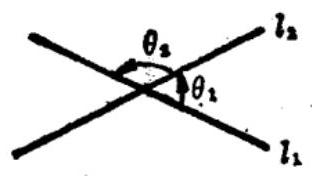
\includegraphics[max width=0.3\textwidth]{images/01912cc2-ffb6-728e-9ae7-b113ff05c64b_46_107087.jpg}
  %\documentclass[tikz, border=5pt]{standalone}
\usetikzlibrary{angles, quotes, shapes.geometric} % 加载角度、引用、直角标记库
\begin{document}
	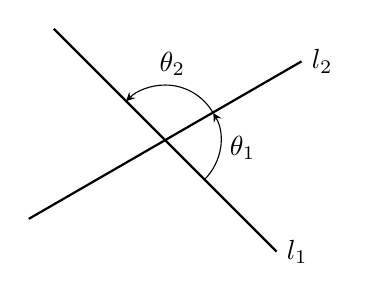
\begin{tikzpicture}[>=stealth, scale=1]
		
		% 1. 绘制直线 \( l_1 \)
		\draw[thick] (0, 0) -- ++(135: 2) ;
		\draw[thick] (0, 0) -- ++(-45: 2) node[ right] {$l_1$};
		% 2. 绘制直线 \( l_2 \)
		\draw[thick] (0, 0) -- ++(30: 2) node[ right] {$l_2$};
		\draw[thick] (0, 0) -- ++(-150: 2) ;
		
		
		% 4. 标记角度 \( \theta_1 \)(\( l_1 \) 与 x 轴正方向的锐角)
		\draw[->] (0.5, -0.5) arc (-45:30:0.7) node[midway, right] {$\theta_1$};
		
		% 5. 标记角度 \( \theta_2 \)(\( l_2 \) 与 x 轴正方向的钝角)
		\draw[->] (0, 0) -- ++(30: 0.7) arc (30:135:0.7) node[midway, above] {$\theta_2$}; 
		
	\end{tikzpicture}
\end{document}

  \caption{图 1-31}
\end{figure}

如果 \(1 + {k}_{1}{k}_{2} = 0\) ,那么 \(\theta = {90}^{ \circ }\) .

下面研究 \(1 + {k}_{1}{k}_{2} \neq 0\) 的情形.

设 \({l}_{1}\text{、}{l}_{2}\) 的倾斜角分别是 \({\alpha }_{1}\) 和 \({\alpha }_{2}\) (图 1-32),

\[
  \operatorname{tg}{\alpha }_{1} = {k}_{1},\;\operatorname{tg}{\alpha }_{2} = {k}_{2}.
\]

\(\because \theta = {\alpha }_{2} - {\alpha }_{1}\) (图 1-32 甲)

或 \(\;\theta = \pi - \left( {{\alpha }_{1} - {\alpha }_{2}}\right) = \pi + \left( {{\alpha }_{2} - {\alpha }_{1}}\right)\)

\(\therefore \operatorname{tg}\theta = \operatorname{tg}\left( {{\alpha }_{2} - {\alpha }_{1}}\right)\)

或 \(\operatorname{tg}\theta = \operatorname{tg}\left\lbrack {\pi + \left( {{\alpha }_{2} - {\alpha }_{1}}\right) }\right\rbrack = \operatorname{tg}\left( {{\alpha }_{2} - {\alpha }_{1}}\right)\) .

\begin{figure}[h]
	\centering
	% 左侧图片:宽度设置为0.45倍文本宽度,预留间距
	\begin{subfigure}[h]{0.45\textwidth}
		\centering
%  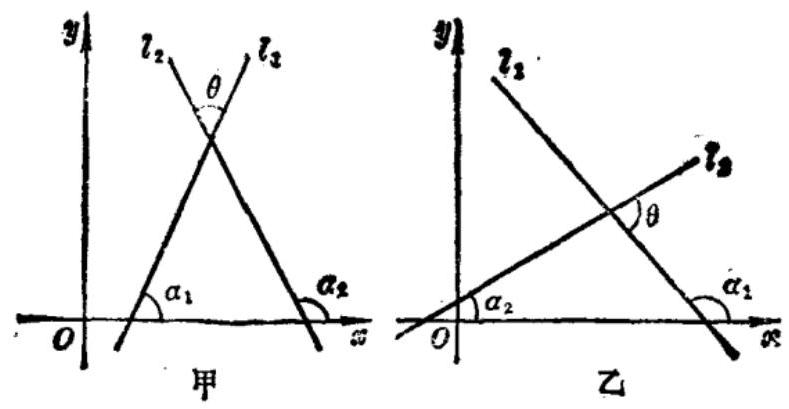
\includegraphics[max width=0.8\textwidth]{images/01912cc2-ffb6-728e-9ae7-b113ff05c64b_47_848929.jpg}
		%\documentclass[tikz, border=5pt]{standalone}
\usetikzlibrary{angles, quotes, shapes.geometric} % 加载角度、引用、直角标记库
\begin{document}
	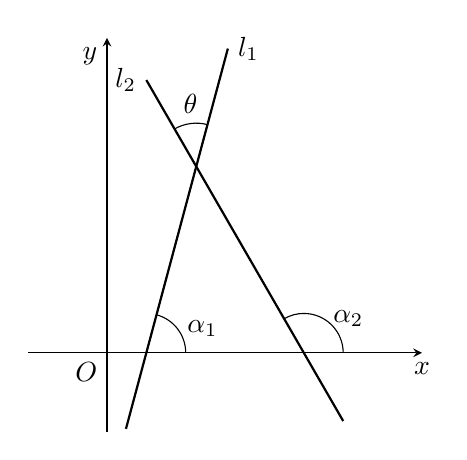
\begin{tikzpicture}[>=stealth, scale=1]
		
		% 1. 绘制坐标轴
		\draw[->] (-1,0) -- (4,0) node[below] {$x$}; % x轴(带箭头和标签)
		\draw[->] (0,-1) -- (0,4) node[below left] {$y$}; % y轴(带箭头和标签)
		\node at (0,0) [below left] {$O$}; % 原点标记
		
		% 2. 绘制直线 \( l_1 \)(倾斜向上)
		\draw[thick] (0.5, 0) --  ++(75: 4) node[right] {$l_1$};
		\draw[thick] (0.5, 0) --  ++(-105: 1) ;
		
		% 3. 绘制直线 \( l_2 \)(倾斜向下,与 \( l_1 \) 垂直)
		\draw[thick] (2.5, 0) -- ++(120: 4) node[ left] {$l_2$};
		\draw[thick] (2.5, 0) -- ++(-60: 1) ;
		
		% 4. 标记角度 \( \alpha_1 \)(\( l_1 \) 与 x 轴正方向的锐角)
		\draw (1, 0) arc (0:75:0.5)  node[midway, right] {$\alpha_1$};
		
		% 5. 标记角度 \( \alpha_2 \)(\( l_2 \) 与 x 轴正方向的钝角)
		\draw (3, 0) arc (0:120:0.5) node[midway, right] {$\alpha_2$}; 
		
		% 6. 绘制夹角标记
		\draw (0.5, 0) --  ++ (75: 3) arc (75:120:0.55) node[midway, above] {$\theta$}; 
		
	\end{tikzpicture}
\end{document}

		\caption{甲}
	\end{subfigure}
	\hfill % 两个图片之间添加空白填充,确保左右分布
	% 右侧图片:宽度设置为0.45倍文本宽度
	\begin{subfigure}[h]{0.45\textwidth}
		\centering
		%\documentclass[tikz, border=5pt]{standalone}
\usetikzlibrary{angles, quotes, shapes.geometric} % 加载角度、引用、直角标记库
\begin{document}
	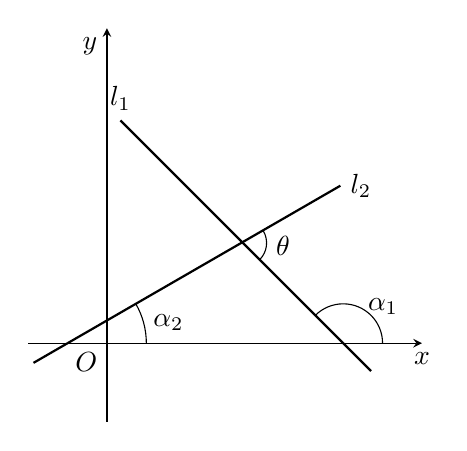
\begin{tikzpicture}[>=stealth, scale=1]
		
		% 1. 绘制坐标轴
		\draw[->] (-1,0) -- (4,0) node[below] {$x$}; % x轴(带箭头和标签)
		\draw[->] (0,-1) -- (0,4) node[below left] {$y$}; % y轴(带箭头和标签)
		\node at (0,0) [below left] {$O$}; % 原点标记
		
		% 2. 绘制直线 \( l_1 \)(倾斜向上)
		\draw[thick] (-0.5, 0) --  ++(30: 4) node[right] {$l_2$};
		\draw[thick] (-0.5, 0) --  ++(-150: 0.5) ;
		
		% 3. 绘制直线 \( l_2 \)(倾斜向下,与 \( l_1 \) 垂直)
		\draw[thick] (3, 0) -- ++(135: 4) node[ above] {$l_1$};
		\draw[thick] (3, 0) -- ++(-45: 0.5) ;
		
		% 4. 标记角度 \( \alpha_1 \)(\( l_1 \) 与 x 轴正方向的锐角)
		\draw (3.5, 0) arc (0:135:0.5) node[midway, right] {$\alpha_1$};
		
		% 5. 标记角度 \( \alpha_2 \)(\( l_2 \) 与 x 轴正方向的钝角)
		\draw (0.5, 0) arc (0:30:1) node[midway, right] {$\alpha_2$}; 
		
		% 6. 绘制夹角标记
		\draw (3, 0) --  ++ (135: 1.5) arc (-45:30:0.3) node[midway, right] {$\theta$}; 
		
	\end{tikzpicture}
\end{document}

		\caption{乙}
	\end{subfigure}
	\caption{图 1-32}
\end{figure}

可得

\[
  \operatorname{tg}\theta = \frac{\operatorname{tg}{\alpha }_{2} - \operatorname{tg}{\alpha }_{1}}{1 + \operatorname{tg}{\alpha }_{2}\operatorname{tg}{\alpha }_{1}}
\]

即

\[
  \operatorname{tg}\theta = \frac{{k}_{2} - {k}_{1}}{1 + {k}_{2}{k}_{1}}.
\]
\begin{corollary}
从一条直线到另一条直线的角, 可能不大于直角, 也可能大于直角, 但我们常常只需要考虑不大于直角的角(就是两条直线所成的角, 简称夹角) 就可以了, 这时可用下面的公式

\[
  \operatorname{tg}\theta = \left| \frac{{k}_{2} - {k}_{1}}{1 + {k}_{2}{k}_{1}}\right| .
\]
\end{corollary}
例 1 求直线 \({l}_{1} : y = - {2x} + 3,\;{l}_{2} : y = x - \frac{3}{2}\) 的夹角.

解: 两条直线的斜率为 \({k}_{1} = - 2,\;{k}_{2} = 1\) ,得

\[
  \operatorname{tg}\theta = \left| \frac{{k}_{2} - {k}_{1}}{1 + {k}_{2}{k}_{1}}\right| = \left| \frac{1 - \left( {-2}\right) }{1 + 1 \cdot \left( {-2}\right) }\right| = 3.
\]

\[
  \therefore \theta = \operatorname{arctg}3 \approx {71}^{ \circ }{34}^{\prime }\text{.}
\]

例 2 已知直线 \({l}_{1} : {A}_{1}x + {B}_{1}y + {C}_{1} = 0\) 和 \({l}_{2} : {A}_{2}x + {B}_{2}y\) \(+ {C}_{2} = 0\left( {{B}_{1} \neq 0\text{、}{B}_{2} \neq 0\text{、}{A}_{1}{A}_{2} + {B}_{1}{B}_{2} \neq 0}\right) ,{l}_{1}\) 到 \({l}_{2}\) 的角是 \(\theta\) . 求证:

\[
  \operatorname{tg}\theta = \frac{{A}_{1}{B}_{2} - {A}_{2}{B}_{1}}{{A}_{1}{A}_{2} + {B}_{1}{B}_{2}}.
\]

证明: 设两条直线 \({l}_{1}\text{、}{l}_{2}\) 的斜率分别为 \({k}_{1}\text{、}{k}_{2}\) ,则

\[
    {k}_{1} = - \frac{{A}_{1}}{{B}_{1}},\;{k}_{2} = - \frac{{A}_{2}}{{B}_{2}}
\]

\[
  \therefore \operatorname{tg}\theta = \frac{{k}_{2} - {k}_{1}}{1 + {k}_{2}{k}_{1}} = \frac{-\frac{{A}_{2}}{{B}_{2}} - \left( {-\frac{{A}_{1}}{{B}_{1}}}\right) }{1 + \left( {-\frac{{A}_{2}}{{B}_{2}}}\right) \left( {-\frac{{A}_{1}}{{B}_{1}}}\right) } = \frac{{A}_{1}{B}_{2} - {A}_{2}{B}_{1}}{{A}_{1}{A}_{2} + {B}_{1}{B}_{2}}\text{.}
\]

例 3 等腰三角形一腰所在的直线 \({l}_{1}\) 的方程是 \(x - {2y}\) \(- 2 = 0\) ,底边所在的直线 \({l}_{2}\) 的方程是 \(x + y - 1 = 0\) ,点 \(\left( {-2,0}\right)\) 在另一腰上,求这腰所在直线 \({l}_{3}\) 的方程.

解: 设 \({l}_{1}\text{、}{l}_{2}\text{、}{l}_{3}\) 的斜率分别为 \({k}_{1}\text{、}{k}_{2}\text{、}{k}_{3},{l}_{1}\) 到 \({l}_{2}\) 的角是 \({\theta }_{1},{l}_{2}\) 到 \({l}_{3}\) 的角是 \({\theta }_{2}\) . 则

\[
    {k}_{1} = \frac{1}{2},\;{k}_{2} = - 1,
\]

\[
  \operatorname{tg}{\theta }_{1} = \frac{{k}_{2} - {k}_{1}}{1 + {k}_{2}{k}_{1}} = \frac{\left( {-1}\right) - \frac{1}{2}}{1 + \left( {-1}\right) \cdot \frac{1}{2}} = - 3.
\]

因为 \({l}_{1}\text{、}{l}_{2}\text{、}{l}_{3}\) 所围成的三角形是等腰三角形,所以

\[
    {\theta }_{1} = {\theta }_{2}
\]

\[
  \operatorname{tg}{\theta }_{2} = \operatorname{tg}{\theta }_{1} = - 3
\]

即

\[
  \frac{{k}_{3} - {k}_{2}}{1 + {k}_{3}{k}_{2}} = - 3
\]

\[
  \frac{{k}_{3} + 1}{1 - {k}_{3}} = - 3
\]

解得

\[
    {k}_{3} = 2\text{.}
\]

因为 \({l}_{3}\) 经过点 \(\left( {-2\text{、}0}\right)\) ,斜率为 2,写出点斜式为

\[
  y = 2\left\lbrack {x - \left( {-2}\right) }\right\rbrack ,
\]

得

\[
    {2x} - y + 4 = 0\text{. }
\]

这就是直线 \({l}_{3}\) 的方程.

\begin{problemset}[练习]

\item 求下列直线 \({l}_{1}\) 到 \({l}_{2}\) 的角与 \({l}_{2}\) 到 \({l}_{1}\) 的角:

(1) \({l}_{1} : y = \frac{1}{2}x + 2,\;{l}_{2} : y = {3x} + 7\) ;

(2) \({l}_{1} : x - y = 5,\;{l}_{2} : x + {2y} - 3 = 0\) .

\item 求下列直线的夹角:

(1) \(y = {3x} - 1,\;y = - \frac{1}{3}x + 4\) ;

(2) \(x - y = 5,\;y = 4\) ;

(3) \({5x} - {3y} = 9,\;{6x} + {10y} + 7 = 0\) .
\end{problemset}

\section{两条直线的交点}

设两条直线的方程是

\[
    {l}_{1} : {A}_{1}x + {B}_{1}y + {C}_{1} = 0,\;{l}_{2} : {A}_{2}x + {B}_{2}y + {C}_{2} = 0.
\]

如果这两条直线相交, 由于交点同时在这两条直线上, 交点的坐标一定是这两个方程的公共解; 反之, 如果这两个二元一次方程只有一个公共解, 那么以这个解为坐标的点必是直线 \({l}_{1}\) 和 \({l}_{2}\) 的交点. 因此,两条直线是否有交点,就要看这两条直线的方程所组成的方程组

\[
  \left\{ \begin{array}{l} {A}_{1}x + {B}_{1}y + {C}_{1} = 0 \\ {A}_{2}x + {B}_{2}y + {C}_{2} = 0 \end{array}\right. \tag{1 2}
\]

是否有唯一解.

设 \({A}_{1}\text{、}{A}_{2}\text{、}{B}_{1}\text{、}{B}_{2}\) 全不为零.

解这个方程组,

(1) \(\times {B}_{2}\) 得 \({A}_{1}{B}_{2}x + {B}_{1}{B}_{2}y + {B}_{2}{C}_{1} = 0\) ,(3)

(2) \(\times {B}_{1}\) 得 \({A}_{2}{B}_{1}x + {B}_{1}{B}_{2}y + {B}_{1}{C}_{2} = 0\) .(4)

(3) \(- \left( 4\right)\) 得 \(\left( {{A}_{1}{B}_{2} - {A}_{2}{B}_{1}}\right) x + {B}_{2}{C}_{1} - {B}_{1}{C}_{2} = 0\) .

下面分两种情形进行讨论:

1. 当 \({A}_{1}{B}_{2} - {A}_{2}{B}_{1} \neq 0\) 时,即 \(\frac{{A}_{1}}{{A}_{2}} \neq \frac{{B}_{1}}{{B}_{2}}\) 时,方程有唯一解:

\[
  \left\{ \begin{array}{l} x = \frac{{B}_{1}{C}_{2} - {B}_{2}{C}_{1}}{{A}_{1}{B}_{2} - {A}_{2}{B}_{1}}, \\ y = \frac{{C}_{1}{A}_{2} - {C}_{2}{A}_{1}}{{A}_{1}{B}_{2} - {A}_{2}{B}_{1}}. \end{array}\right.
\]

这时 \({l}_{1}\) 与 \({l}_{2}\) 相交,上面 \(x\) 和 \(y\) 的值就是交点的坐标.

因为直线 (1) 和 (2) 的斜率分别是 \(- \frac{{A}_{1}}{{B}_{1}}\) 和 \(- \frac{{A}_{2}}{{B}_{2}}\) ,由 \(\frac{{A}_{1}}{{A}_{2}} \neq \frac{{B}_{1}}{{B}_{2}}\) 可得 \(- \frac{{A}_{1}}{{B}_{1}} \neq - \frac{{A}_{2}}{{B}_{2}}\) ,也就是说,两条直线的斜率不相等,它们必相交于一点.

例如, 两条直线的方程是

\[
    {2x} + {3y} - 7 = 0,
\]

\[
    {5x} - y - 9 = 0.
\]

由于 \(\frac{2}{5} \neq \frac{3}{-1}\) ,这两个方程组成的方程组有唯一解,并且这个解是

\[
  \left\{ \begin{array}{l} x = 2 \\ y = 1 \end{array}\right.
\]

就是说,这两条直线相交,交点的坐标是 \(\left( {2,1}\right)\) .

2. 当 \({A}_{1}{B}_{2} - {A}_{2}{B}_{1} = 0\) 时:

(i) 如果 \({B}_{1}{C}_{2} - {B}_{2}{C}_{1} \neq 0\) ,这时 \({C}_{1}\text{、}{C}_{2}\) 不能全为零. 设 \({C}_{2} \neq 0\) ,有 \(\frac{{A}_{1}}{{A}_{2}} = \frac{{B}_{1}}{{B}_{2}} \neq \frac{{C}_{1}}{{C}_{2}}\) . 方程组无解,也就是说这两条直线不相交, 即两直线平行.

因为 \(\frac{{A}_{1}}{{A}_{2}} = \frac{{B}_{1}}{{B}_{2}} \neq \frac{{C}_{1}}{{C}_{2}}\) ,即 \(\frac{{A}_{1}}{{B}_{1}} = \frac{{A}_{2}}{{B}_{2}},\frac{{C}_{1}}{{B}_{1}} \neq \frac{{C}_{2}}{{B}_{2}}\) ,所以直线 (1) 和

(2)的斜率 \(- \frac{{A}_{1}}{{B}_{1}} = - \frac{{A}_{2}}{{B}_{2}}\) ,截距 \(\frac{{C}_{1}}{{B}_{1}} \neq \frac{{C}_{2}}{{B}_{2}}\) ,显然两条直线平行.

例如, 两条直线的方程是

\[
    {2x} - {3y} + 5 = 0,
\]

\[
    {4x} - {6y} - 7 = 0\text{. }
\]

因为 \(\frac{2}{4} = \frac{-3}{-6} \neq \frac{5}{-7}\) ,所以方程组没有解,两条直线平行.

(ii) 如果 \({B}_{1}{C}_{2} - {B}_{2}{C}_{1} = 0\) ,这时 \({C}_{1}\text{、}{C}_{2}\) 或全为零,或全不为零 \(\left( {\text{当 }{C}_{1}\text{、}{C}_{2}\text{ 全不为零时,}\frac{{A}_{1}}{{A}_{2}} = \frac{{B}_{1}}{{B}_{2}} = \frac{{C}_{1}}{{C}_{2}}}\right)\) . 两个方程是同解方程, 因此它们有无穷多解.

这时两条直线的斜率 \(- \frac{{A}_{1}}{{B}_{1}} = - \frac{{A}_{2}}{{B}_{2}}\) ,在 \(y\) 轴上的截距 \(- \frac{{C}_{1}}{{B}_{1}}\) \(= - \frac{{C}_{2}}{{B}_{2}}\) (当 \({C}_{1}\text{、}{C}_{2}\) 全为零时,两条直线都通过原点),两方程的直线重合.

例如, 两条直线的方程是

\[
    {2x} - {3y} + 5 = 0,
\]

\[
    {4x} - {6y} + {10} = 0.
\]

由于 \(\frac{2}{4} = \frac{-3}{-6} = \frac{5}{10}\) ,两个方程是同解方程,方程组有无穷多个解, 两条直线重合.

如果 \({A}_{1}\text{、}{B}_{1}\text{、}{A}_{2}\text{、}{B}_{2}\) 中有等于零的情形,方程比较简单,两条直线的交点很容易讨论.

以上公式较难记忆,以下是geezhu基于通义千问提供的行列式表达:

考虑两条直线:
\[
l_2: A_2x + B_2y + C_2 = 0.
\]
\[
l_2: A_2x + B_2y + C_2 = 0.
\]

我们定义行列式 \(D\) 如下:
\[
  D = \left| \begin{array}{cc}
               A_1 & B_1 \\
               A_2 & B_2
  \end{array} \right| = A_1B_2 - A_2B_1.
\]

如果 \(D \neq 0\),这意味着两条直线在平面上必定相交于一点。此时,\sout{克莱姆法则(Cramer's Rule)}可以用来解出交点坐标:
\[
  x = \frac{D_x}{D}, \quad y = \frac{D_y}{D},
\]
其中:
\[
  D_x = \left| \begin{array}{cc}
                  B_1 & C_1 \\
                  B_2 & C_2
  \end{array} \right|=B_1C_2-B_2C_1\]

\[ \quad
D_y = \left| \begin{array}{cc}
               C_1 & A_1 \\
               C_2 & A_2
\end{array} \right| ==C_1A_2-A_1C_2.
\]

如果 \(D = 0\),这意味着两条直线的系数向量共线,即它们平行或重合。

\begin{enumerate}
  \item 如果 \(D_x = D_y = 0\),这意味着两条直线实际上重合,即它们是同一条直线的不同表示。
  \item 如果 \(D_x \neq 0\) 或 \(D_y \neq 0\),那么两条直线平行但不相交。
\end{enumerate}

例 1 求下列两条直线的交点.

\[
    {l}_{1} : {3x} + {4y} - 2 = 0,
\]

\[
    {l}_{2} : {2x} + y + 2 = 0.
\]

\begin{figure}[h]
  \centering
%  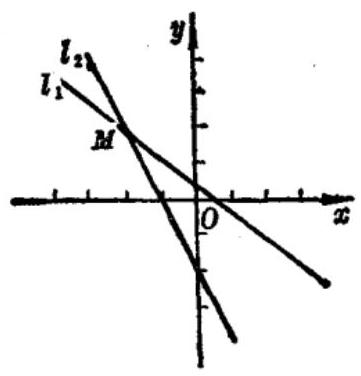
\includegraphics[max width=0.4\textwidth]{images/01912cc2-ffb6-728e-9ae7-b113ff05c64b_52_702387.jpg}
  %\documentclass[tikz, border=5pt]{standalone}
\begin{document}
	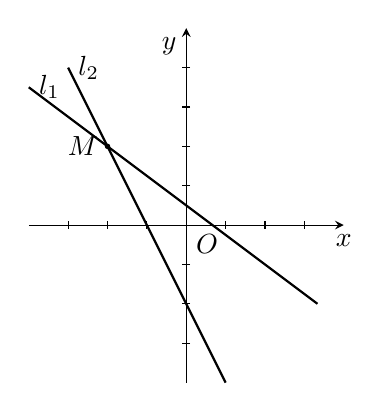
\begin{tikzpicture}[>=stealth, scale=0.5]
		% 1. 绘制坐标轴
		\draw[->] (-4,0) -- (4,0) node[below] {$x$}; % x轴(带箭头和标签)
		\draw[->] (0,-4) -- (0,5) node[below left] {$y$}; % y轴(带箭头和标签)
		\node at (0,0) [below right] {$O$};          % 原点标记
		
		% 绘制所有小刻度线(从 -1 到 2,每隔 1 单位画竖线)
		\foreach \x in {-3,-2,...,3} {
			\draw (\x, 0.1) -- (\x, -0.1) ;  % 小竖线(长 0.2 单位)
		}
	\foreach \y in {-3,-2,...,4} {
		\draw (0.1,\y) -- (-0.1,\y) ;  % 小竖线(长 0.2 单位)
	}
	
	% 2. 绘制直线  l1 虚线 4y=-3x+2 
	\draw[thick] (10/3,-2) -- (-4, 3.5) node[ right] {$l_1$}; % 虚线部分
	% 2. 绘制直线  l 2虚线 y=-2x-2 
	\draw[thick] (1,-4) -- (-3, 4) node[ right] {$l_2$}; % 虚线部分
	
	% 3. 标记各点(M)
	\fill (-2,2) circle (2pt) node [left] {$M$};
	
	\end{tikzpicture}
\end{document}

  \caption{图 1-33}
\end{figure}

解: 解方程组

\[
  \left\{ \begin{array}{l} {3x} + {4y} - 2 = 0 \\ {2x} + y + 2 = 0 \end{array}\right.
\]

得

\[
  \left\{ \begin{array}{l} x = - 2 \\ y = 2 \end{array}\right.
\]

\(\therefore {l}_{1}\) 与 \({l}_{2}\) 的交点是 \(M\left( {-2,2}\right)\) ,如图 1-33.

例 2 已知两条直线:

\[
    {l}_{1} : x + {my} + 6 = 0,
\]

\[
    {l}_{2} : \left( {m - 2}\right) x + {3y} + {2m} = 0.
\]

当 \(m\) 为何值时, \({l}_{1}\) 与 \({l}_{2}\) (i) 相交; (ii) 平行; (iii) 重合.

解: 将两直线的方程组成方程组

\[
  \left\{ \begin{array}{l} x + {my} + 6 = 0, \\ \left( {m - 2}\right) x + {3y} + {2m} = 0. \end{array}\right.
\]

这时, \(\frac{{A}_{1}}{{A}_{2}} = \frac{1}{m - 2},\frac{{B}_{1}}{{B}_{2}} = \frac{m}{3},\frac{{C}_{1}}{{C}_{2}} = \frac{6}{2m}\) .

当 \(\frac{{A}_{1}}{{A}_{2}} = \frac{{B}_{1}}{{B}_{2}}\) 时, \(\frac{1}{m - 2} = \frac{m}{3}\) ,(1)

解得 \(m = - 1\) 或 \(m = 3\) .

当 \(\frac{{A}_{1}}{{A}_{2}} = \frac{{C}_{1}}{{C}_{2}}\) 时, \(\frac{1}{m - 2} = \frac{6}{2m}\) ,(2)

解得

\[
  m = 3\text{.}
\]

(i) 当 \(m \neq - 1\) 且 \(m \neq 3\) 时, \(\frac{{A}_{1}}{{A}_{2}} \neq \frac{{B}_{1}}{{B}_{2}}\) ,方程组有唯一解, \({l}_{1}\) 与 \({l}_{2}\) 相交.

(ii) 当 \(m = - 1\) 时, \(\frac{{A}_{1}}{{A}_{2}} = \frac{{B}_{1}}{{B}_{2}},\frac{{A}_{1}}{{A}_{2}} \neq \frac{{C}_{1}}{{C}_{2}}\) ,方程组无解, \({l}_{1}\) 与 \({l}_{2}\) 平行.

(iii) 当 \(m = 3\) 时, \(\frac{{A}_{1}}{{A}_{2}} = \frac{{B}_{1}}{{B}_{2}} = \frac{{C}_{1}}{{C}_{2}}\) ,方程组有无穷多解, \({l}_{1}\) 与 \({l}_{2}\) 重合.

\begin{problemset}[练习]

\item 求下列各对直线的交点, 并画图:

(1) \({l}_{1} : {2x} + {3y} = {12},{l}_{2} : x - {2y} = 4\) ;

(2) \({l}_{1} : x = 2\) , \(\;{l}_{2} : {3x} + {2y} - {12} = 0\) .

\item 判定下列各对直线的位置关系. 如果相交, 则求出交点的坐标:

(1) \({l}_{1} : {2x} - y = 7,{l}_{2} : {4x} + {2y} = 1\) ;

(2) \({l}_{1} : {2x} - {6y} + 4 = 0,{l}_{2} : y = \frac{x}{3} + \frac{2}{3}\) ;

(3) \({l}_{1} : \left( {\sqrt{2} - 1}\right) x + y = 3,{l}_{2} : x + \left( {\sqrt{2} + 1}\right) y = 2\) .

\item \(A\) 和 \(C\) 取什么值时,直线 \({Ax} - {2y} - 1 = 0\) 和直线 \({6x} - {4y}\) \(+ C = 0\left( 1\right)\) 平行; (2) 重合; (3) 相交.

\end{problemset}

\section{点到直线的距离}

已知点 \(P\left( {{x}_{0},{y}_{0}}\right)\) 和直线 \(l : {Ax} + {By} + C = 0\) ,怎样求点 \(P\) 到直线 \(l\) 的距离呢?

根据定义,点 \(P\) 到直线 \(l\) 的距离是点 \(P\) 到直线 \(l\) 的垂线段的长(图 1-34).

\begin{figure}[h]
	\centering
	% 左侧图片:宽度设置为0.45倍文本宽度,预留间距
	\begin{subfigure}[h]{0.45\textwidth}
		\centering
%		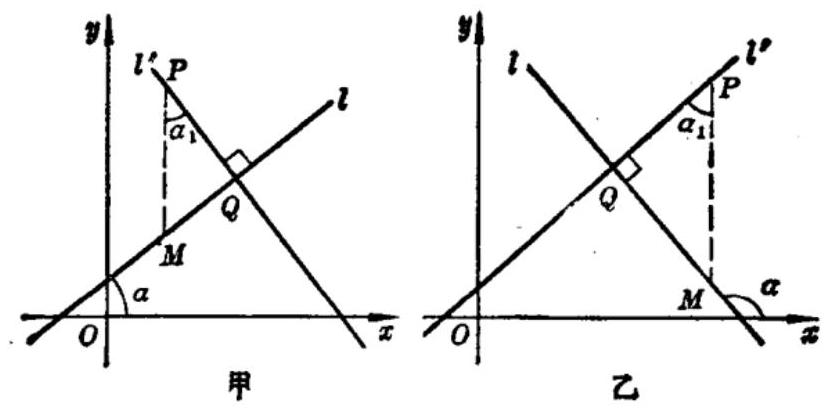
\includegraphics[max width=0.9\textwidth]{images/01912cc2-ffb6-728e-9ae7-b113ff05c64b_54_863018.jpg}
		%\documentclass[tikz, border=5pt]{standalone}
\usetikzlibrary{angles, quotes, shapes.geometric} % 加载角度、引用、直角标记库
\begin{document}
	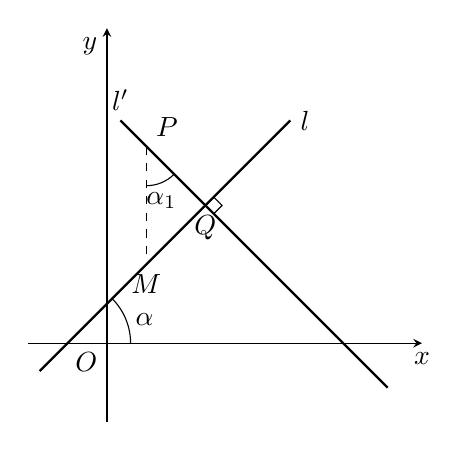
\begin{tikzpicture}[>=stealth, scale=1]
		
		% 1. 绘制坐标轴
		\draw[->] (-1,0) -- (4,0) node[below] {$x$}; % x轴(带箭头和标签)
		\draw[->] (0,-1) -- (0,4) node[below left] {$y$}; % y轴(带箭头和标签)
		\node at (0,0) [below left] {$O$}; % 原点标记
		
		% 2. 绘制直线 \( l \)(倾斜向上)
		\draw[thick] (-0.5, 0) --  ++(45: 4) node[right] {$l$};
		\draw[thick] (-0.5, 0) --  ++(-135: 0.5) ;
		
		% 3. 绘制直线 \( l'\)(倾斜向下,与 \( l \) 垂直)
		\draw[thick] (3, 0) -- ++(135: 4) node[above] {$l'$};
		\draw[thick] (3, 0) -- ++(-45: 0.8) ;
		
		% 4. 标记角度 \( \alpha \)(\( l \) 与 x 轴正方向的锐角)
		\draw (0.3, 0) arc (0:45:0.8)  node[midway, right] {$\alpha$};
		
		% 5. 标记角度 \( \alpha_1\)(\( l' \) 与 x 轴正方向的钝角)
		\draw (0.5, 2) arc (-90:-45:0.5) node[midway, below] {$\alpha_1$}; 
		
		% 6. 绘制直角标记(两直线垂直的符号)
		\draw (1.25, 1.75) -- ++(45: 0.15) -- ++(-45: 0.15)  -- ++(-135: 0.15) ;
		
		% 定义各关键点坐标
		\coordinate (P) at (0.5,2.5);  % 点P₁
		\coordinate (M) at (0.5,1);  % 点M₁
		\coordinate (Q)  at (1.25, 1.75);% 点Q
		
		% 绘制虚线辅助线(矩形的边)
		\draw[dashed] (P) -- (M); % P₁到x轴的虚线
		
		% 标记各点的标签
		\node at (P) [above right]  {$P$};
		\node at (M) [below]          {$M$};
		\node at (Q)  [below]   {$Q$};
		
	\end{tikzpicture}
\end{document}

		\caption{甲}
	\end{subfigure}
	\hfill % 两个图片之间添加空白填充,确保左右分布
	% 右侧图片:宽度设置为0.45倍文本宽度
	\begin{subfigure}[h]{0.45\textwidth}
		\centering
		%\documentclass[tikz, border=5pt]{standalone}
\usetikzlibrary{angles, quotes, shapes.geometric} % 加载角度、引用、直角标记库
\begin{document}
	\begin{tikzpicture}[>=stealth, scale=1]
		
		% 1. 绘制坐标轴
		\draw[->] (-1,0) -- (4,0) node[below] {$x$}; % x轴(带箭头和标签)
		\draw[->] (0,-1) -- (0,4) node[below left] {$y$}; % y轴(带箭头和标签)
		\node at (0,0) [below left] {$O$}; % 原点标记
		
		% 2. 绘制直线 \( l' \)(倾斜向上)
		\draw[thick] (-0.5, 0) --  ++(45: 4.5) node[right] {$l'$};
		\draw[thick] (-0.5, 0) --  ++(-135: 0.5) ;
		
		% 3. 绘制直线 \( l \)(倾斜向下,与 \( l \) 垂直)
		\draw[thick] (3, 0) -- ++(135: 4) node[above] {$l$};
		\draw[thick] (3, 0) -- ++(-45: 0.8) ;
		
		% 4. 标记角度 \( \alpha \)(\( l \) 与 x 轴正方向的锐角)
		\draw (3.5, 0) arc (0:135:0.5)  node[midway, above] {$\alpha$};
		
		% 5. 标记角度 \( \alpha_1\)(\( l' \) 与 x 轴正方向的钝角)
		\draw (2, 2.5) arc (-135:-90:0.35) node[midway, below] {$\alpha_1$}; 
		
		% 6. 绘制直角标记(两直线垂直的符号)
		\draw (1.25, 1.75) -- ++(45: 0.15) -- ++(-45: 0.15)  -- ++(-135: 0.15) ;
		
		% 定义各关键点坐标
		\coordinate (P) at (2.25,2.75);  % 点P₁
		\coordinate (M) at (2.25, 0.75);  % 点M₁
		\coordinate (Q)  at (1.25, 1.75);% 点Q
		
		% 绘制虚线辅助线(矩形的边)
		\draw[dashed] (P) -- (M); % P₁到x轴的虚线
		
		% 标记各点的标签
		\node at (P) [above] {$P$};
		\node at (M) [below] {$M$};
		\node at (Q)  [below] {$Q$};
		
	\end{tikzpicture}
\end{document}

		\caption{乙}
	\end{subfigure}
	\caption{图 1-34}
\end{figure}

设点 \(P\) 到直线 \(l\) 的垂线为 \({l}^{\prime }\) ,垂足为 \(Q\) . 由 \({l}^{\prime } \bot l\) 可知 \({l}^{\prime }\) 的斜率为 \(\frac{B}{A}\left( {A \neq 0}\right)\) ,根据点斜式可写出 \({l}^{\prime }\) 的方程,并由 \(l\) 与 \({l}^{\prime }\) 的方程求出点 \(Q\) 的坐标; 由此即可根据两点距离公式求出 \(\left| {PQ}\right|\) ,这就是点 \(P\) 到直线 \(l\) 的距离.

这个方法虽然思路自然, 但是运算很繁, 下面介绍另一种求法.

设 \(A \neq 0,B \neq 0\) ,直线 \(l\) 的倾斜角为 \(\alpha\) . 过点 \(P\) 作 \({PM}\) \(//{Oy}\) ,那么 \({PM}\) 与 \(l\) 相交于点 \(M\left( {{x}_{1},{y}_{1}}\right)\) (图 1-34).

\[
  \because \;{PM}\parallel {Oy}\text{,}
\]

\[
  \therefore \;{x}_{1} = {x}_{0}\text{. }
\]

代入直线 \(l\) 的方程可得

\[
    {y}_{1} = - \frac{A{x}_{0} + C}{B}
\]

\[
  \therefore \;\left| {PM}\right| = \left| {{y}_{0} - {y}_{1}}\right| = \left| {{y}_{0} + \frac{A{x}_{0} + C}{B}}\right|
\]

\[
  = \frac{\left| A{x}_{0} + B{y}_{0} + C\right| }{\left| B\right| }
\]

当 \(\alpha < {90}^{ \circ }\) 时 (如图 1-34 甲), \({\alpha }_{1} = \alpha\) ;

当 \(\alpha > {90}^{ \circ }\) 时 (如图 1-34 乙), \({\alpha }_{1} = \pi - \alpha\) ,

所以, 在两种情况下都有

\[
    {\operatorname{tg}}^{2}{\alpha }_{1} = {\operatorname{tg}}^{2}\alpha = \frac{{A}^{2}}{{B}^{2}}
\]

\[
  \because \;{\alpha }_{1} < {90}^{ \circ }\text{,}
\]

\[
  \cos {\alpha }_{1} = \frac{1}{\sqrt{1 + {\operatorname{tg}}^{2}{\alpha }_{1}}} = \frac{1}{\sqrt{1 + \frac{{A}^{2}}{{B}^{2}}}}
\]

\[
  = \frac{\left| B\right| }{\sqrt{{A}^{2} + {B}^{2}}}\text{. }
\]

\[
  \therefore \left| {PQ}\right| = \left| {PM}\right| \cos {\alpha }_{1}
\]

\[
  = \frac{\left| A{x}_{0} + B{y}_{0} + C\right| }{\left| B\right| } \cdot \frac{\left| B\right| }{\sqrt{{A}^{2} + {B}^{2}}}
\]

\[
  = \frac{\left| A{x}_{0} + B{y}_{0} + C\right| }{\sqrt{{A}^{2} + {B}^{2}}}.
\]
\begin{corollary}[点到直线的距离公式]
这样,我们就得到平面内一点 \(P\left( {{x}_{0},{y}_{0}}\right)\) 到一条直线 \({Ax} + {By} + C = 0\) 的距离公式:

\[
  \mathbf{d} = \frac{\left| \mathbf{A}{\mathbf{x}}_{0} + \mathbf{B}{\mathbf{y}}_{0} + \mathbf{C}\right| }{\sqrt{{\mathbf{A}}^{2} + {\mathbf{B}}^{2}}}.
\]

如果 \(A = 0\) 或 \(B = 0\) ,上面的距离公式仍然成立. 但这时不需要利用公式就可以直接求出距离.
\end{corollary}
例 1 求点 \({P}_{0}\left( {-1,2}\right)\) 到直线 (i) \({2x} + y - {10} = 0\) ; (ii) \({3x}\) \(= 2\) 的距离.

解: (i) 根据点到直线的距离公式, 得

\[
  d = \frac{\left| 2 \times \left( -1\right) + 1 \times 2 - {10}\right| }{\sqrt{{2}^{2} + {1}^{2}}} = \frac{10}{\sqrt{5}} = 2\sqrt{5}.
\]

(ii) 因为直线 \({3x} = 2\) 平行于 \(y\) 轴,所以

\[
  d = \left| {\frac{2}{3} - \left( {-1}\right) }\right| = \frac{5}{3}.
\]

例 2 求平行线 \({2x} - {7y} + 8 = 0\) 和 \({2x} - {7y} - 6 = 0\) 的距离.

解: 在直线 \({2x} - {7y} - 6 = 0\) 上任取一点,例如取 \(P\left( {3,0}\right)\) (图 1-35),则两平行线的距离就是点 \(P\left( {3,0}\right)\) 到直线

\[
    {2x} - {7y} + 8 = 0
\]

的距离。

因此,

\[
  d = \frac{\left| 2 \times 3 - 7 \times 0 + 8\right| }{\sqrt{{2}^{2} + {\left( -7\right) }^{2}}}
\]

\[
  = \frac{14}{\sqrt{53}} = \frac{{14}\sqrt{53}}{53}
\]

\begin{figure}[h]
	\centering
	%  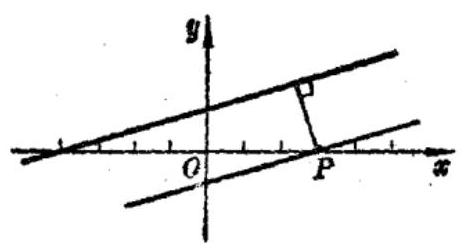
\includegraphics[max width=0.5\textwidth]{images/01912cc2-ffb6-728e-9ae7-b113ff05c64b_56_427717.jpg}
	%\documentclass[tikz, border=5pt]{standalone}
\begin{document}
	\begin{tikzpicture}[>=stealth, scale=0.5] % 箭头样式为stealth,
		
		% 绘制坐标轴
		\draw[->] (-5,0) -- (6,0) node[below] {$x$}; % x轴(带箭头和标签)
		\draw[->] (0,-2) -- (0,3.5) node[below left] {$y$}; % y轴(带箭头和标签)
		\node at (0,0) [below left] {$O$};           % 原点O的标签
		
		% 绘制所有小刻度线(从 -1 到 2,每隔 1 单位画竖线)
		\foreach \x in {-4,-3,...,5} {
			\draw (\x, 0.1) -- (\x, -0.1);  % 小竖线(长 0.2 单位)
		}
		\foreach \y in {-1,0,...,2} {
			\draw (0.1,\y) -- (-0.1,\y);  % 小竖线(长 0.2 单位)
		}
		
		% 绘制直线l 7y=2x+8
		\draw[line width=1pt] (-4.5,-1/7) -- (5,18/7) ;
		% 绘制直线l 7y=2x-6
		\draw[thick] (-2,-10/7) -- (5.5,5/7) ;
		
		% 交点: (131/53, 98/53)
		\draw[thick] (3, 0) -- ++({180-atan(3.5)}:1.95);
		% 直角符号
		\draw (131/53, 98/53) -- ++({atan(2/7)}:0.15) -- ++({atan(2/7)-90}:0.15) -- ++({atan(2/7)-180}:0.15);
%		\draw (2.47, 1.85) -- ++({atan(2/7)}:0.15) -- ++({atan(2/7)-90}:0.15) -- ++({atan(2/7)-180}:0.15);
		
		% 标记各点的标签
		\node at (3,0) [below] {$P$};
		
	\end{tikzpicture}
\end{document}

	\caption{图 1-35}
\end{figure}

\begin{problemset}[练习]

\item 求坐标原点到下列直线的距离:

(1) \({3x} + {2y} - {26} = 0\) ; (2) \(x = y\) .

\item 求下列点到直线的距离:

(1) \(A\left( {-2,3}\right)\) , \({3x} + {4y} + 3 = 0\) ;

(2) \(B\left( {1,0}\right) ,\;\sqrt{3}x + y - \sqrt{3} = 0\) ;

(3) \(C\left( {1, - 2}\right) ,\;{4x} + {3y} = 0\) .

\item 求下列两条平行线的距离:

(1) \({2x} + {3y} - 8 = 0,{2x} + {3y} + {18} = 0\) ;

(2) \({3x} + {4y} = {10},{3x} + {4y} = 0\) .

\end{problemset}

\begin{problemset}[习 题 三]

\item 已知直线分别满足下列条件, 求直线的方程:

(1)经过点 \(A\left( {3,2}\right)\) ,且与直线 \({4x} + y - 2 = 0\) 平行;

(2) 经过点 \(B\left( {3,0}\right)\) ,且与直线 \({2x} + y - 5 = 0\) 垂直;

(3)经过点 \(C\left( {2, - 3}\right)\) ,且平行于过两点 \(M\left( {1,2}\right)\) 和 \(N( - 1\) , \(- 5)\) 的直线.

\item 设有两点 \(A\left( {7, - 4}\right) \text{、}B\left( {-5,6}\right)\) ,求线段 \({AB}\) 的垂直平分线的方程.

\item 三角形三个顶点是 \(A\left( {4,0}\right) \text{、}B\left( {6,7}\right) \text{、}C\left( {0,3}\right)\) . 求这个三角形的三条高所在直线的方程.

\item 已知直线分别满足下列条件, 求直线的方程:

(1)斜率为 -2,且过两条直线 \({3x} - y + 4 = 0\) 和 \(x + y - 4\) . \(= 0\) 的交点;

(2)过两条直线 \(x - {2y} + 3 = 0\) 和 \(x + {2y} - 9 = 0\) 的交点和原点;

(3)经过两条直线 \({2x} - {3y} + {10} = 0\) 和 \({3x} + {4y} - 2 = 0\) 的交点,且垂直于直线 \({3x} - {2y} + 4 = 0\) ;

(4)经过两条直线 \({2x} + y - 8 = 0\) 和 \(x - {2y} + 1 = 0\) 的交点,且平行于直线 \({4x} - {3y} - 7 = 0\) ;

(5) 经过直线 \(y = {2x} + 3\) 和 \({3x} - y + 2 = 0\) 的交点,且垂直. 于第一条直线.

\item 直线 \({ax} + {2y} + 8 = 0,{4x} + 3\dot{y} = {10}\) 和 \({2x} - y = {10}\) 相交于一点. 求 \(a\) 的值.

\item 不解方程组, 判定下列两个方程的直线的位置关系.

(i) \(\left\{ \begin{array}{l} {2x} + y = {11} \\ x + {3y} = {18} \end{array}\right.\) (2) \(\left\{ \begin{array}{l} {2x} - {3y} = 4 \\ {4x} - {6y} = 8 \end{array}\right.\)

(3) \(\left\{ \begin{array}{l} {3x} + {10y} = {16} \\ {6x} + {20y} = 7 \end{array}\right.\) (4) \(\left\{ \begin{array}{l} {4x} + {10y} = {12} \\ {6x} - {15y} = {18} \end{array}\right.\)

\item 已知两条直线

\({l}_{1};\;\left( {3 + m}\right) x + {4y} = 5 - {3m},\)

\({l}_{2} : {2x} + \left( {5 + m}\right) y = 8.\)

\(m\) 为何值时, \({l}_{1}\) 与 \({l}_{2}\left( 1\right)\) 相交; (2) 平行; (3) 重合.

\item 讨论两条直线 \({l}_{1} : {A}_{1}x + {B}_{1}y + {C}_{1} = 0,{l}_{2} : {A}_{2}x + {B}_{2}y + {C}_{2}\) \(= 0\) 的位置关系: (1) 当 \({B}_{1} = 0,{B}_{2} \neq 0\) 时; (2) 当 \({B}_{1} = {B}_{2}\) \(= 0\) 时.

\item 三角形的三个顶点是 \(A\left( {6,3}\right) \text{、}B\left( {9,3}\right) \text{、}C\left( {3,6}\right)\) . 求它的三个内角的度数.

\item 已知直线 \(l\) 经过点 \(P\left( {2,1}\right)\) ,且和直线 \({5x} + {2y} + 3 = 0\) 的夹角等于 \({45}^{ \circ }\) . 求直线 \(l\) 的方程.

\item 光线从点 \(M\left( {-2,3}\right)\) 射到 \(x\) 轴上一点 \(P\left( {1,0}\right)\) 后被 \(x\) 轴反射. 求反射光线所在直线的方程.

\item 求点 \(P\left( {-5,7}\right)\) 到直线 \({12x} + {5y} - 3 = 0\) 的距离.

\item 点 \(A\left( {a,6}\right)\) 到直线 \({3x} - {4y} = 2\) 的距离 (1) 等于 4 ; (2) 大于 4. 分别求 \(a\) 的值.

\item 求证: 两条平行线 \({Ax} + {By} + {C}_{1} = 0\) 与 \({Ax} + {By} + {C}_{2} = 0\) 的距离是

\[
  d = \frac{\left| {C}_{1} - {C}_{2}\right| }{\sqrt{{A}^{2} + {B}^{2}}}
\]

\item 求两条平行线 \({3x} - {2y} - 1 = 0\) 和 \({6x} - {4y} + 2 = 0\) 的距离.

\end{problemset}

\chapter*{小 结}
\markboth{小 结}{小 结}

一、在这一章里, 我们首先研究了有向线段、两点的距离及线段的定比分点; 接着又研究了直线方程的各种形式, 并利用这些方程讨论了两条直线的位置关系和两条直线所成的角、点到直线的距离. 这种通过方程研究图形性质的方法就是解析法. 解析法揭示了数学中“数”和“形”的内在联系.

二、有向线段的数量、两点的距离与定比分点等公式是解析几何的基本公式. 在用解析法研究点的轨迹问题时, 经常用到这些公式.

三、本章介绍了点斜式、斜截式; 两点式、截距式等直线方程的特殊形式, 并研究了直线方程的一般式, 这些直线的方程都是二元一次方程. 每一个二元一次方程都表示一条直线; 反之, 表示每一条直线的方程都是二元一次方程. 但是表示同一条直线的方程形式却不是唯一的, 不过它们都可以通过方程的同解变形互化, 可以看作是同一个方程. 就这个意义来说, 直线和二元一次方程是一一对应的.

四、直线的斜率和截距是表示直线位置的重要特征数值, 通过它们可以判定两条直线的位置关系: 平行、相交 (包括垂直)及重合。

在斜截式 \(y = {kx} + b\) 中,如果 \(k\) 固定, \(b\) 取不同的值时,我们得到一组平行的直线; 在点斜式方程 \(y - {y}_{0} = k\left( {x - {x}_{0}}\right)\) 中, \(k\) 取不同的值时,则得到过定点 \(A\left( {{x}_{0},{y}_{0}}\right)\) 的一组直线.

*五、二元一次不等式表示区域和直线型经验公式在生产与科学研究中都常常用到. 利用二元一次不等式表示的区域, 我们还可以确定一个点与直线的位置关系. 把点 \(P\left( {{x}_{0},{y}_{0}}\right)\) 的坐标代入直线方程 \({Ax} + {By} + C = 0\) 的左边,由 \(A{x}_{0} + B{y}_{0} + C\) 的值的正负可以确定点 \(P\) 是在该直线的上方还是下方.

六、在研究了直线方程的各种形式之后, 本章还研究了两条直线的交点、夹角以及点到直线的距离等问题. 我们除了要掌握这些问题的结论外, 还应注意学习通过代数方程研究几何性质的方法.

\chapter*{复习参考题一}
\markboth{复习参考题一}{复习参考题一}

\section*{A 组}

1. 已知 \(\bigtriangleup {ABC}\) 顶点的坐标是 \(A\left( {2,3}\right) \text{、}B\left( {5,3}\right) \text{、}C\left( {2,7}\right)\) . 求 \(\angle A\) 的平分线长及所在直线的方程.

2. 已知矩形的顶点为 \(O\left( {0,0}\right) \text{、}A\left( {8,0}\right) \text{、}B\left( {0,5}\right)\) . 试用两种方法求两条对角线所在直线的方程.

3. 用两种方法证明: 三点 \(A\left( {-2,{12}}\right) \text{、}B\left( {1,3}\right) \text{、}C\left( {4, - 6}\right)\) 在同一条直线上.

4. 求直线 \({2x} - {5y} - {10} = 0\) 和坐标轴所围成的三角形的面积.

5. 求经过点 \(A\left( {-3,4}\right)\) ,并且在两轴上截距的和等于 12 的直线的方程.

*6. 在 \(x,y\) 的坐标都不小于 0 的整数点中,求满 足 \(x + y \leq 4\) 的点的个数.

*7. 一定量的气体,在一定压强下体积 \(V\left( {\mathrm{\;{cm}}}^{3}\right)\) 和温度 \(T\left( {{}^{ \circ }\mathrm{C}}\right)\) 之间关系的实验数据如下:

\begin{center}
  \adjustbox{max width=\textwidth}{
    \begin{tabular}{|c|c|c|c|c|c|c|}
      \hline
      \(T\) (℃) & 20 & 30 & 40 & 50 & 60 & 70 \\
      \hline
      \(V\) (cm3) & 106.5 & 110.9 & 114.0 & 117.2 & 121. 2 & 124.7 \\
      \hline
    \end{tabular}
  }
\end{center}

用选点法求出 \(V\) 与 \(T\) 间的经验公式.

*8. 一个 10 欧姆的电阻, 使用不同的电压通电, 量得电流数值如下:

\begin{center}
  \adjustbox{max width=\textwidth}{
    \begin{tabular}{|c|c|c|c|c|c|c|}
      \hline
      电压 \(V\) (伏特) & 5 & 10 & 15 & 20 & 25 & 30 \\
      \hline
      电流 \(I\) (安培) & 0.55 & 1. 14 & 1. 45 & 2. 10 & 2. 45 & 3.10 \\
      \hline
    \end{tabular}
  }
\end{center}

用平均值法求出 \(I\) 与 \(V\) 间的经验公式.

9. 已知平行四边形两条边所在直线的方程是

\[
  x + y - 1 = 0,{3x} - y + 4 = 0,
\]

它的对角线的交点是 \(M\left( {3,3}\right)\) . 求这个平行四边形其他两边的方程.

10. 直线 \(\left( {{3a} + 2}\right) x + \left( {1 - {4a}}\right) y + 8 = 0\) 和 \(\left( {{5a} - 2}\right) x + \left( {a + 4}\right) y\) \(- 7 = 0\) 互相垂直. 求 \(a\) 的值.

11. \({ABCD}\) 是正方形, \(E\text{、}F\text{、}G\text{、}H\) 分别是边 \({AB}\text{、}{BC}\text{、}{CD}\text{、}{DA}\) 的中点. 求证:

(1)线段 \({AF}\text{、}{BG}\text{、}{CH}\text{、}{DE}\) 围成一个正方形;

(2)这个正方形的面积是原正方形面积的 \(\frac{1}{5}\) .

12. (1) 当 \(a\) 为何值时,下列两方程的直线平行:

(i) \({ax} - {5y} = 9,\;{2x} - {3y} = {15}\) ;

(ii) \(x + {2ay} - 1 = 0,\;\left( {{3a} - 1}\right) x - {ay} - 1 = 0\) ;

(iii) \({2x} + {3y} = a,\;{4x} + {6y} - 3 = 0\) .

(2)当 \(m\text{、}n\) 各为何值时,下列两方程的直线重合:

(i) \(x + {2y} = 4,\;{mx} + y = n\) ;

(ii) \({mx} + {10y} = 2,\;{3x} + \left( {n - 1}\right) y = - 1\) .

(3)当 \(a\) 为何值时,下列两方程的直线互相垂直:

(i) \({4ax} + y = 1,\left( {1 - a}\right) x + y = - 1\) ;

(ii) \({2x} + {ay} = 2,\;{ax} + {2y} = 1\) .

13. 已知两条直线

\({l}_{1} : x + \left( {1 + m}\right) y = 2 - m,\;{l}_{2} : {2mx} + {4y} = - {16}.\)

当 \(m\) 为何值时, \({l}_{1}\) 与 \({l}_{2}\left( 1\right)\) 相交; (2) 平行; (3) 重合.

14. 求两条平行直线 \({3x} + {4y} - {12} = 0\) 和 \({6x} + {8y} + {11} = 0\) 的距离.

15. 求平行于直线 \(x - y - 2 = 0\) 且与它的距离为 \(2\sqrt{2}\) 的直线方程.

16. 正方形的中心在 \(C\left( {-1,0}\right)\) ,一条边所在的直线方程是 \(x + {3y} - 5 = 0\) ,求其他三边所在的直线方程.

\section*{B 组}

17. 已知: 直线 \(l : {Ax} + {By} + C = 0\left( {A \neq 0,B \neq 0}\right)\) ,点 \(M\left( {x}_{0}\right.\) , \(\left. {y}_{0}\right)\) . 求证: (1) 经过点 \(M\) 且平行于直线 \(l\) 的直线方程是 \(A\left( {x - {x}_{0}}\right) + B\left( {y - {y}_{0}}\right) = 0\) ; (2) 经过点 \(M\) 且垂直于直线 \(l\) 的直线的方程是 \(\frac{x - {x}_{0}}{A} = \frac{y - {y}_{0}}{B}\) .

18. 已知平行直线 \({3x} + {2y} - 6 = 0\) 与 \({6x} + {4y} - 3 = 0\) . 求与它们等距离的平行线的方程.

19. 一条光线从点 \({M}_{0}\left( {5,3}\right)\) 射出后,被直线 \(l : x + y = 1\) 反射,入射光线到直线 \(l\) 的角为 \(\beta\) . 已知 \(\operatorname{tg}\beta = 2\) ,求入射光线与反射光线所在直线的方程.

20. 直线 \({l}_{1}\text{、}{l}_{2}\text{、}{l}_{3}\) 的方程分别是

\({l}_{1} : {A}_{1}x + {B}_{1}y + {C}_{1} = 0;\)

\({l}_{2} : {A}_{2}x + {B}_{2}y + {C}_{2} = 0;\)

\({l}_{3} : {A}_{1}x + {B}_{1}y + {C}_{1} + \lambda \left( {{A}_{2}x + {B}_{2}y + {C}_{2}}\right) = 0.\)

如果当 (1) \({l}_{1}\) 和 \({l}_{2}\) 相交; (2) \({l}_{1}\) 和 \({l}_{2}\) 平行时,直线 \({l}_{3}\) 和 \({l}_{1}\text{、}{l}_{2}\) 的位置关系如何?

21. 山顶上有高 \(h\) 的塔 \({BC}\) ,从塔顶 \(B\) 测得地面上一点 \(A\) 的俯角是 \(\alpha\) ,从塔底 \(C\) 测得点 \(A\) 的俯角是 \(\beta\) ,用解析法求山高 \(H\) .

\begin{figure}[h]
  \centering
%  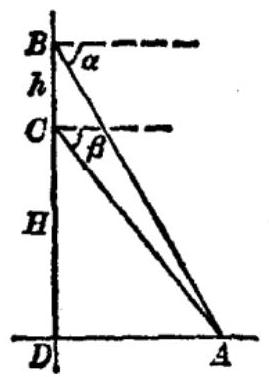
\includegraphics[max width=0.3\textwidth]{images/01912cc2-ffb6-728e-9ae7-b113ff05c64b_64_551024.jpg}
  %\documentclass[tikz, border=5pt]{standalone}
\begin{document}
	\begin{tikzpicture}[>=stealth, scale=1]
		% 绘制坐标轴
		\draw[->] (-1,0) -- (3,0) ; % x轴(带箭头和标签)node[below] {$x$}
		\draw[->] (0,-1) -- (0,4) ; % y轴(带箭头和标签)node[below left] {$y$}
		\node at (0,0) [below left] {$D$};           % 原点O的标签
		
		% 直线
		\draw[thick] (2, 0) -- (0, 2) ; 
		\draw[thick] (2, 0) -- ++(120:4) ; 
		
		% 绘制虚线辅助线
		\draw[dashed] (0,{2*tan(60)}) -- (1.5,{2*tan(60)});  % B的虚线
		\draw[dashed] (0,2) -- (1.5,2);  % C的虚线
		
		% 标记各点的标签
		\node at (2,0) [below] {$A$};
		\node at (0,2) [ left] {$C$};
		\node at (0,{2*tan(60)}) [ left] {$B$};
		
		\node at (0,1) [left] {$H$};
		\node at (0,2.8)  [left] {$h$};
		
		%  弧线
		\draw (0.5, {2*tan(60)}) arc (0:-60:0.5) node[midway, right] {$\alpha$}; 
		\draw (0.5, 2) arc (0:-45:0.5) node[midway, right] {$\beta$}; 
		
	\end{tikzpicture}
\end{document}

  \caption{(第 21题)}
\end{figure}

22. 过两点 \(A\left( {-3,2}\right)\) 和 \(B\left( {6,1}\right)\) 的直线与直线 \(x + {3y} - 6 = 0\) 交于点 \(P\) . 求点 \(P\) 分 \(\overline{AB}\) 所成的比.


\chapter{圆 锥 曲 线}

\section*{一\text{ }曲线和方程}

\section{曲线和方程}

在第一章里, 我们研究过直线的各种方程, 讨论了直线和二元一次方程的关系. 下面, 我们进一步研究一般曲线 (包括直线) 和方程的关系.

我们知道, 两坐标轴所成的角在第一、三象限的平分线的方程是 \(x - y = 0\) ,就是说,如果点 \(M\left( {{x}_{0},{y}_{0}}\right)\) 是这条直线上的任意一点,它到两坐标轴的距离一定相等,即 \({x}_{0} = {y}_{0}\) ,那么它的坐标 \(\left( {{x}_{0},{y}_{0}}\right)\) 是方程 \(x - y = 0\) 的解; 反过来,如果 \(\left( {{x}_{0},{y}_{0}}\right)\) 是方程 \(x - y = 0\) 的解,即 \({x}_{0} = {y}_{0}\) ,那么以这个解为坐标的点到两轴的距离相等,它一定在这条平分线上. 这样,我们就说 \(x - y = 0\) 是这条平分线的方程.

又如,函数 \(y = a{x}^{2}\) 的图象是关于 \(y\) 轴对称的抛物线,这条抛物线是所有以方程 \(y = a{x}^{2}\) 的解为坐标的点组成的. 这就是说,如果 \(M\left( {{x}_{0},{y}_{0}}\right)\) 是抛物线上的点,那么 \(\left( {{x}_{0},{y}_{0}}\right)\) 一定是这个方程的解; 反过来,如果 \(\left( {{x}_{0},{y}_{0}}\right)\) 是方程 \(y = a{x}^{2}\) 的解,那么以它为坐标的点一定在这条抛物线上. 这样,我们就说 \(y = a{x}^{2}\) 是这条抛物线的方程.

\begin{corollary}[曲线和方程的关系]	
一般地,在直角坐标系中,如果某曲线 \(C\) (看作适合某种条件的点的集合或轨迹) 上的点与一个二元方程 \(f\left( {x,y}\right) = 0\) 的实数解建立了如下的关系:

1. 曲线上的点的坐标都是这个方程的解;

2. 以这个方程的解为坐标的点都是曲线上的点,

那么,这个方程叫做曲线的方程;这条曲线叫做方程的曲线 (图形).
\end{corollary}

例  证明以坐标原点为圆心, 半径等于 5 的圆的方程是 \({x}^{2} + {y}^{2} = {25}\) ,并判断点 \( {M}_{1} \left( {3, - 4} \right) \) ,\( {M}_{2} \left(  {-2\sqrt{5},2} \right) \) 是否在这个圆上。

证明: 1. 设 \(M\left( {{x}_{0},{y}_{0}}\right)\) 是圆上任意一点. 因为点 \(M\) 到坐标原点的距离等于 5 , 所以

\[
  \sqrt{{x}_{0}^{2} + {y}_{0}^{2}} = 5
\]

也就是

\[
    {x}_{0}^{2} + {y}_{0}^{2} = {25}
\]

即 \(\left( {{x}_{0},{y}_{0}}\right)\) 是方程 \({x}^{2} + {y}^{2} = {25}\) 的解.

2. 设 \(\left( {{x}_{0},{y}_{0}}\right)\) 是方程 \({x}^{2} + {y}^{2} = {25}\) 的解,那么

\[
    {x}_{0}^{2} + {y}_{0}^{2} = {25}\text{.}
\]

两边开方取算术根, 得

\[
  \sqrt{{x}_{0}^{2} + {y}_{0}^{2}} = 5\text{.}
\]

\begin{figure}[h]
  \centering
%  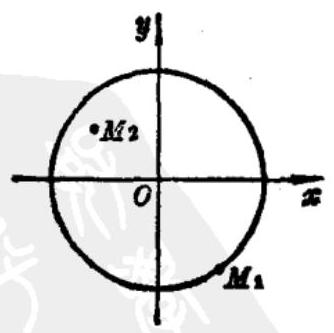
\includegraphics[max width=0.3\textwidth]{images/01912cc2-ffb6-728e-9ae7-b113ff05c64b_66_677276.jpg}
  %\documentclass[tikz, border=5pt]{standalone}
\usetikzlibrary{angles, quotes} % 用于绘制角度标记
\begin{document}
	\begin{tikzpicture}[>=stealth, scale=0.5] % 缩放使图形更清晰
		
		% 绘制坐标轴
		\draw[->] (-5,0) -- (5,0) node[below] {$x$};
		\draw[->] (0,-5) -- (0,5) node[below left] {$y$};
		
		% 绘制圆
		\draw[thick] (0,0) circle (4);
		
		\fill ({4*cos(-60)}, {4*sin(-60)}) circle (2pt) node[ right] {$M_1$}; % 圆上的交点
		\fill(-2,2) circle (2pt) node[ right] {$M_2$}; 
		
	\end{tikzpicture}
\end{document}

  \caption{图 2-1}
\end{figure}

即点 \(M\left( {{x}_{0},{y}_{0}}\right)\) 到坐标原点的距离等于 5,点 \(M\left( {{x}_{0},{y}_{0}}\right)\) 是这个圆上的点.

“这里少了,这里少了,这里少了,”

\[
    {x}^{2} + {y}^{2} = {25}
\]

“这里少了,这里少了,这里少了,” 圆心,半径等 “这里少了,这里少了,这里少了,” 

(3, -4) 的坐标代入方程 \({x}^{2} + {y}^{2} = {25}\) ,左右两边相等, \(\left( {3, - 4}\right)\) 是方程的解,所以点 \({M}_{1}\) 在这个圆上;

把 \({M}_{2}\left( {-2\sqrt{5},2}\right)\) 的坐标代入方程 \({x}^{2} + {y}^{2} = {25}\) ,左右两边不等, \(\left( {-2\sqrt{5},2}\right)\) 不是方程的解,所以点 \({M}_{2}\) 不在这个圆上 (如图 2-1).

\begin{problemset}[练习]

\item 到两坐标轴距离相等的点组成的直线的方程是 \(x - y = 0\) 吗? 为什么?

\item 已知等腰三角形三个顶点的坐标是 \(A\left( {0,3}\right) ,B\left( {-2,0}\right)\) , \(C\left( {2,0}\right)\) . 中线 \({AO}\) 的方程是 \(x = 0\) 吗? 为什么?

\end{problemset}

\section{求曲线的方程}

我们先看两个例子.

例 1 设 \(A\text{、}B\) 两点的坐标是 \(\left( {-1, - 1}\right) \text{、}\left( {3,7}\right)\) ,求线段 \({AB}\) 的垂直平分线的方程。

\begin{figure}[h]
  \centering
%  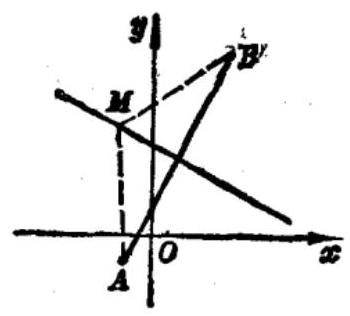
\includegraphics[max width=0.4\textwidth]{images/01912cc2-ffb6-728e-9ae7-b113ff05c64b_67_837628.jpg}
  %\documentclass[tikz, border=5pt]{standalone}
\begin{document}
	\begin{tikzpicture}[>=stealth, scale=0.5]
		% 绘制坐标轴
		\draw[->] (-4,0) -- (6,0) node[below] {$x$}; % x轴(带箭头和标签)
		\draw[->] (0,-2) -- (0,8) node[below left] {$y$}; % y轴(带箭头和标签)
		\node at (0,0) [below right] {$O$};           % 原点O的标签
		
		% 直线l  x+2y−7=0
		\draw[thick] (-3, 5) -- (5, 1) node[above right] {$l$}; 
		
		% 定义各关键点坐标
		\coordinate (A) at (-1,-1);  % 点P₁
		\coordinate (B) at (3,7); % 点P₂
		\coordinate (M) at (-1,4);  % 点M₁
		
		% 绘制连线
		\draw[thick] (A) -- (B);  % Q到P₁的虚线
		\draw[dashed] (A) -- (M); % P₁到x轴的虚线
		\draw[dashed] (B) -- (M); % P₂到y轴的虚线
		
		% 标记各点的标签
		\fill (A) circle (2pt) node[below] {$A$};  % 绘制点A
		\fill (B) circle (2pt) node[right] {$B$};   % 绘制点B
		\fill (M) circle (2pt) node[above] {$M$};    % 绘制点M
		
	\end{tikzpicture}
\end{document}

  \caption{图 2-2}
\end{figure}

解: 设 \(M\left( {x,y}\right)\) 是线段 \({AB}\) 的垂直平分线上任意一点 (图 2-2), 也就是点 \(M\) 属于集合

\[
  P = \{ M\left| \right| {MA}\left| = \right| {MB} \mid \} .
\]

由两点的距离公式,点 \(M\) 所适合的条件可表示为

\[
  \sqrt{{\left( x + 1\right) }^{2} + {\left( y + 1\right) }^{2}} = \sqrt{{\left( x - 3\right) }^{2} + {\left( y - 7\right) }^{2}}.
\]

两边平方后, 得

\[
    {\left( x + 1\right) }^{2} + {\left( y + 1\right) }^{2} = {\left( x - 3\right) }^{2} + {\left( y - 7\right) }^{2},
\]

即

\[
  x + {2y} - 7 = 0\text{. } \tag{1}
\]

下面,我们证明方程 (1) 是线段 \({AB}\) 的垂直平分线的方程.

1. 由上面求方程的过程可知, 垂直平分线上每一点的坐标都是方程 (1) 的解;

2. 设点 \({M}_{1}\) 的坐标 \(\left( {{x}_{1},{y}_{1}}\right)\) 是方程 (1) 的解,即

\[
    {x}_{1} + 2{y}_{1} - 7 = 0,
\]

\[
    {x}_{1} = 7 - 2{y}_{1}
\]

点 \({M}_{1}\) 到 \(A\text{、}B\) 的距离分别是

\[
  \left| {{M}_{1}A}\right| = \sqrt{{\left( {x}_{1} + 1\right) }^{2} + {\left( {y}_{1} + 1\right) }^{2}}
\]

\[
  = \sqrt{{\left( 8 - 2{y}_{1}\right) }^{2} + {\left( {y}_{1} + 1\right) }^{2}}
\]

\[
  = \sqrt{5\left( {{y}_{1}^{2} - 6{y}_{1} + {13}}\right) }\text{;}
\]

\[
  \left| {{M}_{1}B}\right| = \sqrt{{\left( {x}_{1} - 3\right) }^{2} + {\left( {y}_{1} - 7\right) }^{2}}
\]

\[
  = \sqrt{{\left( 4 - 2{y}_{1}\right) }^{2} + {\left( {y}_{1} - 7\right) }^{2}}
\]

\[
  = \sqrt{5\left( {{y}_{1}^{2} - 6{y}_{1} + {13}}\right) }\text{.}
\]

\[
  \therefore \;\left| {{M}_{1}A}\right| = \left| {{M}_{1}B}\right| \text{,}
\]

即点 \({M}_{1}\) 在线段 \({AB}\) 的垂直平分线上.

由上述证明可知,方程 (1) 是线段 \({AB}\) 的垂直平分线的方程。

例 2 点 \(M\) 与两条互相垂直的直线的距离的积是常数 \(k\left( {k > 0}\right)\) ,求点 \(M\) 的轨迹方程。

\begin{figure}[h]
  \centering
%  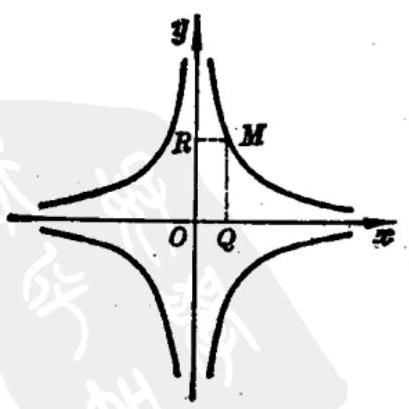
\includegraphics[max width=0.4\textwidth]{images/01912cc2-ffb6-728e-9ae7-b113ff05c64b_68_272250.jpg}
  %\documentclass[tikz, border=5pt]{standalone}
\begin{document}
	\begin{tikzpicture}[>=stealth, scale=0.5]
		% 1. 绘制坐标轴
		\draw[->] (-4,0) -- (4,0) node[below] {$x$};  % x轴(带箭头和标签)
		\draw[->] (0,-4) -- (0,4) node[below left] {$y$};  % y轴(带箭头和标签)
		\node at (0,0) [below left] {$O$};  % 原点标记
		
		% 2. 绘制双曲线(以 \( xy = 1 \) 和 \( xy = -1 \) 为例,控制“张开程度”)
		% 第一、三象限分支:\( xy = 1 \)
		\draw[thick, domain=0.3:3, smooth, variable=\x] plot (\x, {1/\x});   % 右支
		\draw[thick, domain=-3:-0.3, smooth, variable=\x] plot (\x, {1/\x}); % 左支
		% 第二、四象限分支:\( xy = -1 \)
		\draw[thick, domain=0.3:3, smooth, variable=\x] plot (\x, {-1/\x});  % 右支
		\draw[thick, domain=-3:-0.3, smooth, variable=\x] plot (\x, {-1/\x}); % 左支
		
		% 3. 标记点与辅助线(以 \( M(1,1) \) 为例)
		\coordinate (Q) at (1,0);  % 点Q(x轴上)
		\coordinate (R) at (0,1);  % 点R(y轴上)
		\coordinate (M) at (1,1);  % 点M(双曲线上)
		
		% 绘制虚线辅助线(MQ垂直x轴,MR垂直y轴)
		\draw[dashed] (M) -- (Q);
		\draw[dashed] (M) -- (R);
		
		% 标记点标签
		\node at (Q) [below] {$Q$};
		\node at (R) [left] {$R$};
		\node at (M) [above right] {$M$};
	\end{tikzpicture}
\end{document}

  \caption{图 2-3}
\end{figure}

解: 取已知两条互相垂直的直线为坐标轴, 建立直角坐标系(图 2-3).

设点 \(M\) 的坐标为 \(\left( {x,y}\right)\) . 点 \(M\) 的轨迹就是与坐标轴的距离的积是常数 \(k\) 的点的集合

\[
  P = \{ M\left| \right| {MR}\left| \cdot \right| {MQ} \mid = k\} ,
\]

其中 \(Q\text{、}R\) 分别是点 \(M\) 到 \(x\) 轴、 \(y\) 轴的垂线的垂足.

因为点 \(M\) 到 \(x\) 轴、 \(y\) 轴的距离,分别是它的纵坐标和横坐标的绝对值,所以条件 \(\left| {MR}\right| \cdot \left| {MQ}\right| = k\) 可写成

\[
  \left| x\right| \cdot \left| y\right| = k
\]

即

\[
    {xy} = \pm k\text{.} \tag{1}
\]

下面我们证明方程 (1) 是所求轨迹的方程.

1. 由上面求方程的过程可知, 曲线上的点的坐标都是方程 (1) 的解;

2. 设点 \({M}_{1}\) 的坐标 \(\left( {{x}_{1},{y}_{1}}\right)\) 是方程 (1) 的解,那么

\[
    {x}_{1}{y}_{1} = \pm k
\]

即

\[
  \left| {x}_{1}\right| \cdot \left| {y}_{1}\right| = k\text{. }
\]

而 \(\left| {x}_{1}\right| \text{、}\left| {y}_{1}\right|\) 正是点 \({M}_{1}\) 到纵轴、横轴的距离,因此点 \({M}_{1}\) 到这两条直线的距离的积是常数 \(k\) ,点 \({M}_{1}\) 在方程 (1) 的曲线上.

由 1、2 可知, 方程 (1) 是所求轨迹的方程. 图形如图 \(2 - 3\) .

由上面的例子可以看出, 求曲线 (图形) 的方程, 一般有下面几个步骤:

(1)建立适当的直角坐标系,用 \(\left( {x,y}\right)\) 表示曲线上任意一点 \(M\) 的坐标;

(2)写出适合条件 \(p\) 的点 \(M\) 的集合 \(P = \{ M \mid p\left( M\right) \}\) ;

(3)用坐标表示条件 \(p\left( M\right)\) ,列出方程 \(f\left( {x,y}\right) = 0\) ;

(4)化方程 \(f\left( {x,y}\right) = 0\) 为最简形式;

(5)证明以化简后的方程的解为坐标的点都是曲线上的点.

除个别情况外, 化简过程都是同解变形过程, 步骤(5)可以省略不写, 如有特殊情况, 可适当予以说明. 另外, 根据情况, 也可以省略步骤 (2), 直接列出曲线方程.

例 3 已知一条曲线在 \(x\) 轴的上方,它上面的每一点,到点 \(A\left( {0,2}\right)\) 的距离减去它到 \(x\) 轴的距离的差都是 2,求这条曲线的方程.

解: 设点 \(M\left( {x,y}\right)\) 是曲线上任意一点, \({MB} \bot x\) 轴,垂足是 \(B\) (图 2-4),那么点 \(M\) 属于集合

\[
  P = \{ M\left| \right| {MA}\left| -\right| {MB} \mid = 2\} \text{. }
\]

由距离公式,点 \(M\) 适合的条件可表示为

\[
  \sqrt{{x}^{2} + {\left( y - 2\right) }^{2}} - y = 2. \tag{1}
\]

将 (1) 式移项后再两边平方, 得

\[
    {x}^{2} + {\left( y - 2\right) }^{2} = {\left( y + 2\right) }^{2},
\]

化简得

\[
  y = \frac{1}{8}{x}^{2}.
\]

\begin{figure}[h]
	\centering
	%  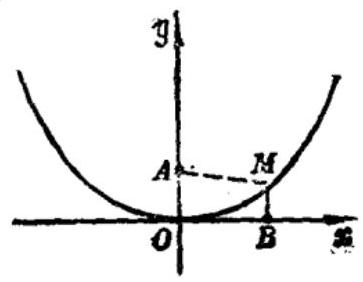
\includegraphics[max width=0.4\textwidth]{images/01912cc2-ffb6-728e-9ae7-b113ff05c64b_70_664169.jpg}
	%\documentclass[tikz, border=5pt]{standalone}
\begin{document}
	\begin{tikzpicture}[>=stealth, scale=0.6]
		% 1. 绘制坐标轴
		\draw[->] (-5,0) -- (5,0) node[below] {$x$};  % x轴
		\draw[->] (0,-1) -- (0,3) node[below left] {$y$};% y轴
		\node at (0,0) [below left] {$O$};            % 原点标记
		
		% 2. 绘制抛物线 \(8y = x^2\)(即 \(y = \frac{x^2}{8}\))
		\draw[thick, domain=-4.5:4.5, smooth, variable=\x] 
		plot ({\x}, {\x*\x/8});
		
		% 3. 定义并标记关键点
		\coordinate (A) at (0, 2);  % 点A(y轴上)
		\coordinate (B) at (3, 0);    % 点B(x轴上)
		\coordinate (M) at (3, 9/8);  % 点M(抛物线上,\(x=2\) 时 \(y=\frac{2^2}{8}=0.5\))
		
		% 4. 绘制辅助线
		\draw[dashed] (A) -- (M);  % 虚线连接A和M
		\draw[thick] (M) -- (B);   % 实线连接M和B(垂直x轴)
		
		% 5. 标记点(实心小圆+标签)
		\fill (A) circle (1.5pt) node[left] {$A$};
		\fill (B) circle (1.5pt) node[below] {$B$};
		\fill (M) circle (1.5pt) node[above] {$M$};
	\end{tikzpicture}
\end{document}

	\caption{图 2-4}
\end{figure}

因为曲线在 \(x\) 轴的上方, \(y > 0\) ,虽然原点 \(O\) 的坐标 \(\left( {0,0}\right)\) 是这个方程的解, 但不属于已知曲线, 所以曲线的方程应是 \(y = \frac{1}{8}{x}^{2}\left( {x \neq 0}\right)\) ,它的图形是关于 \(y\) 轴对称的抛物线 (图2-4), 但缺一个顶点.

求出曲线方程以后, 我们就可以根据曲线的方程, 来研究曲线的几何性质, 这个问题, 我们将在后面结合各种具体的曲线方程来说明.

\begin{problemset}[练习]

\item 求到坐标原点的距离等于 2 的点的轨迹方程.

\item 已知点 \(M\) 与 \(x\) 轴的距离和它与点 \(F\left( {0,4}\right)\) 的距离相等,求点 \(M\) 的轨迹方程。

\end{problemset}

\section{充要条件}

从 2.1 节我们知道, \(y = a{x}^{2}\) 是一条抛物线的方程。这就是说,如果点 \(M\) 的坐标是方程 \(y = a{x}^{2}\) 的解,那么点 \(M\) 一定是这条抛物线上的点.

象这样,我们就说 “点 \(M\) 的坐标是方程 \(y = a{x}^{2}\) 的解”是 “点 \(M\) 在这条抛物线上”的充分条件.

又如, 如果一个三角形有两个角相等, 那么这个三角形是等腰三角形.

同样, 我们说 “有两个角相等”是“三角形是等腰三角形” 的充分条件.

\begin{definition}[充分条件]
一般地,如果 \(A\) 成立,那么 \(B\) 成立,即 \(A \Rightarrow B\) ,这时我们就说条件 \(A\) 是 \(B\) 成立的充分条件. 也就是说,为使 \(B\) 成立,具备条件 \(A\) 就足够了.
\end{definition}

再举一些充分条件的例子:

(1)如果不重合的两条直线 \({l}_{1}\text{、}{l}_{2}\) 的斜率 \({k}_{1} = {k}_{2}\) ,那么 \({l}_{1}//{l}_{2}\) . 因此, \({k}_{1} = {k}_{2}\) 是 \({l}_{1}//{l}_{2}\) 的充分条件.

(2)如果 \(x = y\) ,那么 \({x}^{2} = {y}^{2}\) . 因此, \(x = y\) 是 \({x}^{2} = {y}^{2}\) 的充分条件.

(3)如果两个三角形全等, 那么这两个三角形面积相等. 因此, 两个三角形全等是两个三角形面积相等的充分条件.

从 2.1 节我们还知道,如果点 \(M\) 在方程 \(y = a{x}^{2}\) 的曲线上,那么点 \(M\) 的坐标一定是方程 \(y = a{x}^{2}\) 的解.

象这样,我们就说 “点 \(M\) 的坐标是方程 \(y = a{x}^{2}\) 的解” 是 “点 \(M\) 在抛物线上”的必要条件.

又如, 如果三角形是等腰的, 那么它有两个角相等.

同样, 我们说“有两个角相等”是“三角形是等腰三角形” 的必要条件.

\begin{definition}[必要条件]
一般地,如果 \(B\) 成立,那么 \(A\) 成立,即 \(B \Rightarrow A\) ,或者,如果 \(A\) 不成立,那么 \(B\) 就不成立,这时我们就说,条件 \(A\) 是 \(B\) 成立的必要条件. 也就是说,要使 \(B\) 成立,就必须 \(A\) 成立.
\end{definition}

\begin{corollary}[逆否命题等价性]
  因为 “ \(B \Rightarrow A\) ”和它的逆否命题 “ \(\bar{A} \Rightarrow \bar{B}\) ” 是等价的,所以,如果 \(A\) 不成立,那么 \(B\) 就一定不成立,也就是说,要使 \(\bar{B}\) 成立, \(\bar{A}\) 就必须成立.
\end{corollary}

再举一些必要条件的例子:

(1)如果两条有斜率的直线 \({l}_{1}//{l}_{2}\) ,那么它们的斜率 \({k}_{1}\) \(= {k}_{2}\) ,也就是,如果 \({k}_{1} \neq {k}_{2}\) ,那么 \({l}_{1}\) 与 \({l}_{2}\) 不平行. 因此, \({k}_{1} = {k}_{2}\) 是 \({l}_{1}//{l}_{2}\) 的必要条件.

(2)如果 \(x = y\) ,那么 \({x}^{2} = {y}^{2}\) . 也就是,如果 \({x}^{2} \neq {y}^{2}\) ,那么 \(x \neq y\) . 因此, \({x}^{2} = {y}^{2}\) 是 \(x = y\) 的必要条件.

(3)如果两个三角形全等, 那么这两个三角形的面积相等, 也就是, 如果两个三角形的面积不相等, 那么它们不能全等. 因此, 两个三角形面积相等是它们全等的必要条件.

综上所述,我们看到,如果 \(A \Rightarrow B\) ,那么 \(A\) 是 \(B\) 成立的充分条件; 如果 \(B \Rightarrow A\) ,那么 \(A\) 是 \(B\) 成立的必要条件.
\begin{definition}[充要条件]
  有时既有 \(A \Rightarrow B\) ,又有 \(B \Rightarrow A\) ,那么 \(A\) 既是 \(B\) 成立的充分条件,又是 \(B\) 成立的必要条件. 这时,我们就说 \(A\) 是 \(B\) 成立的充分而且必要的条件, 简称充要条件.
\end{definition}
例如,如果 \(f\left( {x,y}\right) = 0\) 是曲线 \(C\) 的方程,那么“点 \(M\) 的坐标是方程 \(f\left( {x,y}\right) = 0\) 的解” 就是 “点 \(M\) 在曲线 \(C\) 上” 的充要条件; “有两个角相等”就是“三角形是等腰三角形”的充要条件; “两条有斜率的直线 \({l}_{1}\text{、}{l}_{2}\) 的斜率 \({k}_{1} = {k}_{2}\) ”就是“ \({l}_{1}//{l}_{2}\) ”的充要条件.

应该注意, 对于某个结论来说, 有的条件是充分条件, 但不是必要条件; 也有的条件是必要条件, 但不是充分条件.

例如," \(x = y\) "是 “ \(x = y\) ” 的充分条件,但不是必要条件. 因为要使 \({x}^{2} = {y}^{2}\) ,不一定要有 \(x = y\) ,有 \(x = - y\) 也可以了.

又如, 两个三角形面积相等是它们全等的必要条件, 但不是充分条件. 因为得出两个三角形全等, 只有面积相等是不够的.

充要条件是进一步学习时常用的数学概念之一.

\begin{problemset}[练习]

\item “ \(b = 0\) ” 是 “直线 \(y = {kx} + b\) 过原点” 的什么条件,为什么?

\item “四边相等”是 “一个四边形是正方形” 的什么条件, 为什么?

\item “ \(x - 1 = 0\) ” 是 “ \({x}^{2} - 1 = 0\) ” 的什么条件,为什么?

\item “两条直线不相交”是“这两条直线异面”的什么条件, 为什么?
\end{problemset}

\section{曲线的交点}

由曲线方程的定义可知, 两条曲线交点的坐标应该是两个曲线方程的公共实数解, 即两个曲线方程组成的方程组的实数解; 反过来, 方程组有几个实数解, 两条曲线就有几个交点, 方程组没有实数解, 两条曲线就没有交点. 即两条曲线有交点的充要条件是它们的方程所组成的方程组有实数解. 可见, 求曲线的交点的问题, 就是求由它们的方程所组成的方程组的实数解的问题.

例 1 求直线 \(y = x + \frac{3}{2}\) 被曲线 \(y = \frac{1}{2}{x}^{2}\) 截得的线段的长.

\begin{figure}[h]
  \centering
%  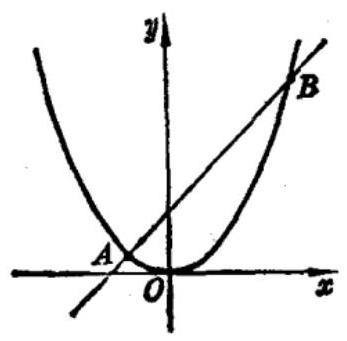
\includegraphics[max width=0.4\textwidth]{images/01912cc2-ffb6-728e-9ae7-b113ff05c64b_74_639219.jpg}
  %\documentclass[tikz, border=5pt]{standalone}
\begin{document}
	\begin{tikzpicture}[>=stealth, scale=0.5]
		% 1. 绘制坐标轴
		\draw[->] (-3, 0) -- (4, 0) node[below] {$x$};
		\draw[->] (0, -1) -- (0, 6) node[below left] {$y$};
		\node at (0, 0) [below left] {$O$};  % 标记原点
		
		% 2. 绘制抛物线 \( 2y = x^2 \)(即 \( y = \frac{x^2}{2} \))
		\draw[thick, domain=-3:3.3, smooth, variable=\x]
		plot (\x, {\x*\x / 2});
		
		% 3. 绘制直线 \( y = x + 1.5 \)
		\draw[thick, domain=-2:4]
		plot (\x, {\x + 1.5});
		
		% 4. 标记交点 \( A(-1, 0.5) \) 和 \( B(3, 4.5) \)
		\fill (-1, 0.5) circle (2pt) node[ left] {$A$};
		\fill (3, 4.5) circle (2pt) node[ right] {$B$};
	\end{tikzpicture}
\end{document}

  \caption{图 2-5}
\end{figure}

解: 先求交点.

解方程组

\[
  \left\{ \begin{array}{l} y = x + \frac{3}{2} \\ y = \frac{1}{2}{x}^{2} \end{array}\right.
\]

得

\[
  \left\{ {\begin{array}{l} {x}_{1} = - 1, \\ {y}_{1} = \frac{1}{2}; \end{array}\;\left\{ \begin{array}{l} {x}_{2} = 3, \\ {y}_{2} = \frac{9}{2}. \end{array}\right. }\right.
\]

所以交点 \(A\text{、}B\) 的坐标分别是 \(\left( {-1,\frac{1}{2}}\right) \text{、}\left( {3,\frac{9}{2}}\right)\) . 直线被曲线截得的线段长

\[
  \left| {AB}\right| = \sqrt{{\left( 3 + 1\right) }^{2} + {\left( \frac{9}{2} - \frac{1}{2}\right) }^{2}} = 4\sqrt{2}.
\]

例 2 已知某圆的方程是 \({x}^{2} + {y}^{2} = 2\) 。当 \(b\) 为何值时,直线 \(y = x + b\) 与圆有两个交点;两个交点重合为一点;没有交点?

\begin{figure}[h]
  \centering
%  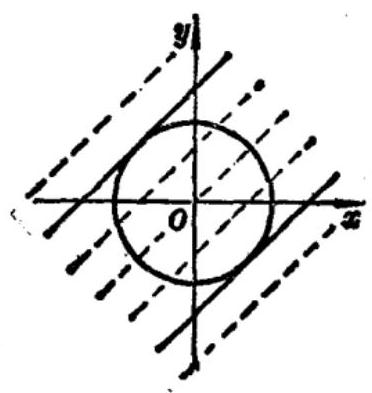
\includegraphics[max width=0.4\textwidth]{images/01912cc2-ffb6-728e-9ae7-b113ff05c64b_75_443692.jpg}
  %\documentclass[tikz, border=5pt]{standalone}
\begin{document}
	\begin{tikzpicture}[>=stealth, scale=0.8] % 缩放使图形更清晰
		% 1. 绘制坐标轴
		\draw[->] (-3,0) -- (3,0) node[below] {$x$};
		\draw[->] (0,-3) -- (0,3) node[below left] {$y$};
		\node at (0,0) [below left] {$O$};  % 原点标记
		
		% 绘制圆
		\draw[thick] (0,0) circle (1.4);
		
		% 绘制线
		\draw[thick] (-0.5, -2.5) -- (2.5, 0.5) ; 
		\draw[thick] (-2.5, -0.5) -- (0.5, 2.5) ; 
		
		% 绘制虚线
		\draw[dashed] (-2, -1) -- (1, 2) ; 
		\draw[dashed] (-1.5, -1.5) -- (1.5, 1.5) ; 
		\draw[dashed] (-1, -2) -- (2, 1) ; 
		\draw[dashed] (-3,0) -- (0,3); 
		\draw[dashed] (0,-3) -- (3,0); 
		
	\end{tikzpicture}
\end{document}

  \caption{图 2-6}
\end{figure}

解: 解方程组

\[
  \left\{ \begin{array}{l} y = x + b \\ {x}^{2} + {y}^{2} = 2 \end{array}\right. \tag{1 2}
\]

把 (1) 式代入 (2) 式, 得

\[
    {x}^{2} + {\left( x + b\right) }^{2} = 2,
\]

\[
  2{x}^{2} + {2bx} + {b}^{2} - 2 = 0. \tag{3}
\]

方程 (3) 的根的判别式

\[
  \Delta = {\left( 2b\right) }^{2} - 4 \times 2\left( {{b}^{2} - 2}\right)
\]

\[
  = 4\left( {-{b}^{2} + 4}\right)
\]

\[
  = 4\left( {2 + b}\right) \left( {2 - b}\right) \text{.}
\]

当 \(- 2 < b < 2\) 时, \(\Delta > 0\) ,这时方程组有两个不同的实数解, 因此直线与圆有两个交点;

当 \(b = - 2\) 或 \(b = 2\) 时, \(\Delta = 0\) ,这时方程组有两个相同的实数解, 因此直线与圆的两个交点重合为一点;

当 \(b > 2\) 或 \(b < - 2\) 时, \(\Delta < 0\) ,这时方程组没有实数解,因此直线与圆没有交点.

实际上,上述三种情况,就是直线与圆相交、相切、相离 (图 2-6)。

\begin{problemset}[练习]

\item 求直线 \({2x} - {5y} + 5 = 0\) 与曲线 \(y = - \frac{10}{x}\) 的交点.
\end{problemset}

\begin{problemset}[习 题 四]

\item 点 \(A\left( {1, - 2}\right) \text{、}B\left( {2, - 3}\right) \text{、}C\left( {3,{10}}\right)\) 是否在方程

\[
    {x}^{2} - {xy} + {2y} + 1 = 0
\]

的图形上?

\item (1) 在什么情况下,方程 \(y = a{x}^{2} + {bx} + c\) 的曲线经过原点?

(2) 在什么情况下,方程 \({\left( x - a\right) }^{2} + {\left( y - b\right) }^{2} = {r}^{2}\) 的曲线经过原点?

\item 已知点 \(M\) 到 \(x\) 轴、 \(y\) 轴的距离的乘积等于 1 . 求点 \(M\) 的轨迹方程.

\item 点 \(M\) 到点 \(A\left( {4,0}\right)\) 和点 \(B\left( {-4,0}\right)\) 的距离的和为 12,求点 \(M\) 的轨迹方程.

\item 一个点到点 \(\left( {4,0}\right)\) 的距离等于它到 \(y\) 轴的距离,求这个点的轨迹方程.

\item 两个定点的距离为 6,点 \(M\) 到这两个定点的距离的平方和为 26,求点 \(M\) 的轨迹方程.

\item 求与点 \(O\left( {0,0}\right)\) 和 \(A\left( {c,0}\right)\) 的距离的平方差为常数 \(c\) 的点的轨迹方程.

\begin{figure}[h]
  \centering
  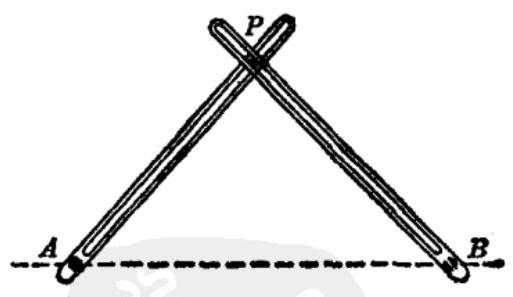
\includegraphics[max width=0.5\textwidth]{images/01912cc2-ffb6-728e-9ae7-b113ff05c64b_76_433068.jpg}
  \caption{(第 8 题)}
\end{figure}

\item 两根杆分别绕着定点 \(A\) 和 \(B\left( {{AB} = {2a}}\right)\) 在平面内转动, 并且转动时两杆保持相互垂直, 求杆的交点 \(P\) 的轨迹方程.

\item 在下列括弧中填写: “充分条件”或“必要条件” 或 “充要条件”:

(1) “ \(m\) 是有理数” 是 “ \(m\) 是实数” 的 ( );

(2) “ \({x}^{2} - 1 = 0\) ” 是 “ \(x - 1 = 0\) ” 的 ( );

(3) “ \(x = {2}^{n}\) 是 “ \({x}^{2} - {5x} + 6 = 0\) ” 的 ( );

(4) “ \(x < 5\) ” 是 “ \(x < 3\) ” 的 ( );

(5) “内错角相等”是 “二直线平行” 的 ( );

(6) “ABCD 是矩形”是 “ABCD 是平行四边形”的 ( );

(7) “两边和夹角对应相等”是 “三角形全等” 的 ( ).

\item 求直线 \({4x} - {3y} = {20}\) 和圆 \({x}^{2} + {y}^{2} = {25}\) 的交点.

\item 求经过两条曲线 \({x}^{2} + {y}^{2} + {3x} - y = 0\) 和 \(3{x}^{2} + 3{y}^{2} + {2x} + y\) \(= 0\) 交点的直线的方程.
\end{problemset}

\section*{二\text{ }圆}

\section{圆的标准方程}

\begin{definition}[圆] 
我们知道, 平面内与定点距离等于定长的点的集合 (轨迹) 是圆. 定点就是圆心, 定长就是半径。
\end{definition}

根据圆的定义, 我们来求圆心是 \(C\left( {a,b}\right)\) ,半径是 \(r\) 的圆的方程 (图 2-7)。

\begin{figure}[h]
  \centering
%  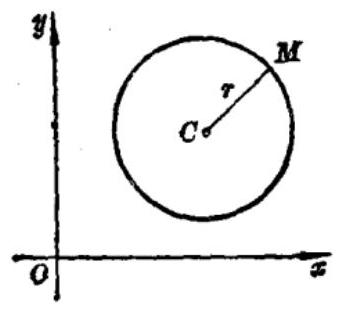
\includegraphics[max width=0.4\textwidth]{images/01912cc2-ffb6-728e-9ae7-b113ff05c64b_77_682858.jpg}
  %\documentclass[tikz, border=5pt]{standalone}
\begin{document}
	\begin{tikzpicture} [>=stealth, scale=1]
		% 1. 绘制坐标轴
		\draw[->] (-0.5,0) -- (4,0) node[below] {$x$};  % x轴
		\draw[->] (0,-0.5) -- (0,4) node[below left] {$y$};  % y轴
		\node at (0,0) [below left] {$O$};  % 标记原点
		
		% 2. 绘制圆(圆心C(2,2),半径1.5)
		\draw (2,2) circle (1.5);
		\node at (2,2) [ left] {$C$};  % 标记圆心
		
		% 3. 绘制半径线段CM并标记
		\draw (2,2) -- (3.5,2) node[midway, above] {$r$};  % 半径线段
		\node at (3.5,2) [above right] {$M$};  % 标记圆上点M
		
	\end{tikzpicture}
\end{document}

  \caption{图 2-7}
\end{figure}

设 \(M\left( {x,y}\right)\) 是圆上任意一点,根据定义,点 \(M\) 到圆心 \(C\) 的距离等于 \(r\) . 圆就是集合

\[
  P = \{ M\} \mid {MC} \mid = r\} .
\]

由两点的距离公式,点 \(M\) 适合的条件可表示为

\[
  \sqrt{{\left( x - a\right) }^{2} + {\left( y - b\right) }^{2}} = r. \tag{1}
\]

把 (1) 式两边平方, 得

\[
    {\left( x - a\right) }^{2} + {\left( y - b\right) }^{2} = {r}^{2}. \tag{2}
\]

方程 (2) 就是圆心是 \(C\left( {a,b}\right)\) ,半径是 \(r\) 的圆的方程。我们把它叫做圆的标准方程。

\begin{definition}[圆的标准方程]
	如果圆心在坐标原点,这时 \(a = 0,b = 0\) ,那么圆的方程就是
	\[
	{x}^{2} + {y}^{2} = {r}^{2}
	\]
\end{definition}

例 1  已知两点 \({P}_{1}\left( {4,9}\right)\) 和 \({P}_{2}\left( {6,3}\right)\) ,求以 \({P}_{1}{P}_{2}\) 为直径的圆的方程,并且判断点 \(M\left( {6,9}\right) \text{、}N\left( {3,3}\right) \text{、}Q\left( {5,3}\right)\) 是在圆上,在圆内,还是在圆外。

解:根据已知条件,圆心 \(C\left( {a,b}\right)\) 是 \({P}_{1}{P}_{2}\) 的中点,那么它的坐标为

\[
  a = \frac{4 + 6}{2} = 5,\;b = \frac{9 + 3}{2} = 6.
\]

再根据两点的距离公式,得圆的半径是

\[
  r = \left| {C{P}_{1}}\right| = \sqrt{{\left( 4 - 5\right) }^{2} + {\left( 9 - 6\right) }^{2}} = \sqrt{10}.
\]

因此所求圆的方程是

\[
    {\left( x - 5\right) }^{2} + {\left( y - 6\right) }^{2} = {10}.
\]

分别计算点 \(M\left( {6,9}\right) \text{、}N\left( {3,3}\right) \text{、}Q\left( {5,3}\right)\) 与圆心 \(C\left( {5,6}\right)\) 的距离,得

\[
  \left| {CM}\right| = \sqrt{{\left( 6 - 5\right) }^{2} + {\left( 9 - 6\right) }^{2}} = \sqrt{10},
\]

\[
  \left| {CN}\right| = \sqrt{{\left( 3 - 5\right) }^{2} + {\left( 3 - 6\right) }^{2}} = \sqrt{13} > \sqrt{10},
\]

\[
  \left| {CQ}\right| = \sqrt{{\left( 5 - 5\right) }^{2} + {\left( 3 - 6\right) }^{2}} = 3 < \sqrt{10},
\]

因此,点 \(M\) 在圆上,点 \(N\) 在圆外,点 \(Q\) 在圆内。

例 2 求以 \(C\left( {1,3}\right)\) 为圆心,并且和直线 \({3x} - {4y} - 7 = 0\) 相切的圆的方程。

解: 已知圆心是 \(C\left( {1,3}\right)\) ,那么只要再求出圆的半径 \(r\) ,就能写出圆的方程。

因为圆 \(C\) 和直线 \({3x} - {4y} - 7 = 0\) 相切,所以半径 \(r\) 等于圆心 \(C\) 到这条直线的距离。根据点到直线的距离公式,得

\[
  r = \frac{\left| 3 \times 1 - 4 \times 3 - 7\right| }{\sqrt{{3}^{2} + {\left( -4\right) }^{2}}} = \frac{16}{5}.
\]

因此,所求的圆的方程是

\[
    {\left( x - 1\right) }^{2} + {\left( y - 3\right) }^{2} = \frac{256}{25}
\]

例 3  已知圆的方程是 \({x}^{2} + {y}^{2} = {r}^{2}\) ,求经过圆上一点 \(M\left( {{x}_{0},{y}_{0}}\right)\) 的切线的方程。

\begin{figure}[h]
	\centering
	%  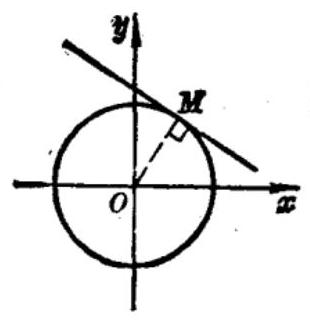
\includegraphics[max width=0.3\textwidth]{images/01912cc2-ffb6-728e-9ae7-b113ff05c64b_79_916236.jpg}
	%\documentclass[tikz, border=5pt]{standalone}
\begin{document}
	\begin{tikzpicture}[>=stealth, scale=0.6]
		% 绘制坐标轴
		\draw[->] (-3,0) -- (4,0) node[below ] {$x$};
		\draw[->] (0,-3) -- (0,4) node[below left] {$y$};
		\node at (0,0) [below left] {$O$};
		
		% 绘制圆(圆心在原点,半径设为2)
		\draw (0,0) circle (2);
		
		% 定义切点M的坐标(M(√2, √2),在圆上且位于第一象限)
		\coordinate (M) at ({sqrt(2)},{sqrt(2)});
		
		% 绘制从原点到切点M的线段(虚线)
		\draw[dashed] (0,0) -- (M);
		
		% 绘制切线(过M且与OM垂直,斜率为-1)
		\draw[thick] (M) -- ++({-sqrt(3)},{sqrt(3)}) (M) -- ++({sqrt(3)},{-sqrt(3)});
		
		% 标记切点M
		\node at (M) [above right] {$M$};
		
		% 绘制直角符号
		\draw ({sqrt(2)},{sqrt(2)}) -- ++ (-45: 0.15) -- ++ (-135: 0.15) -- ++ (135: 0.15) ;
		
	\end{tikzpicture}
\end{document}

	\caption{图 2-8}
\end{figure}

解:如图 2-8,设切线的斜率为 \(k\) ,半径 \({OM}\) 的斜率为 \({k}_{1}\) 。因为圆的切线垂直于过切点的半径,于是 \(k = - \frac{1}{{k}_{1}}\) 。

\[
    {k}_{1} = \frac{{y}_{0}}{{x}_{0}}
\]

\[
  \therefore \;k = - \frac{{x}_{0}}{{y}_{0}}\text{. }
\]

经过点 \(M\) 的切线方程是

\[
  y - {y}_{0} = - \frac{{x}_{0}}{{y}_{0}}\left( {x - {x}_{0}}\right)
\]

整理得

\[
    {x}_{0}x + {y}_{0}y = {x}_{0}^{2} + {y}_{0}^{2}
\]

\begin{corollary}[切线方程]
因为点 \(M\left( {{x}_{0},{y}_{0}}\right)\) 在圆上,所以 \({x}_{0}^{2} + {y}_{0}^{2} = {r}^{2}\) ,所求切线方程是
\[
    {x}_{0}x + {y}_{0}y = {r}^{2}
\]
\end{corollary}

例 4     图 2-9 是某圆拱桥的一孔圆拱的示意图. 该圆拱跨度 \({AB} = {20}\) 米,拱高 \({OP} = 4\) 米,在建造时每隔 4 米需用一个支柱支撑,求支柱 \({A}_{2}{P}_{2}\) 的长度 (精确到 0.01 米)。

\begin{figure}[h]
	\centering
	%  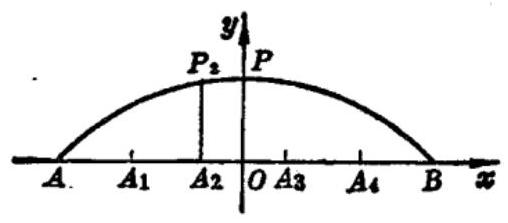
\includegraphics[max width=0.5\textwidth]{images/01912cc2-ffb6-728e-9ae7-b113ff05c64b_80_540621.jpg}
	%\documentclass[tikz, border=5pt]{standalone}
\begin{document}
	\begin{tikzpicture}[>=stealth, scale=0.5] % 箭头样式为stealth,
		
		% 绘制坐标轴
		\draw[->] (-6,0) -- (6,0) node[below] {$x$}; % x轴(带箭头和标签)
		\draw[->] (0,-1) -- (0,3) node[ left] {$y$}; % y轴(带箭头和标签)
		\node at (0,0) [below right] {$O$};           % 原点O的标签
		
		% 绘制所有小刻度线(从 -1 到 2,每隔 1 单位画竖线)
		\foreach \x in {-5,-3,...,5} {
			\draw (\x, 0.1) -- (\x, -0.1) ;  % 小竖线(长 0.2 单位)
		}
		
		% 绘制拱形
		\draw[line width=1pt] (5, 0) arc (45:135:7.1) ;\\
		
		% 定义各关键点坐标
		\coordinate (A_2) at (-1,0);  % 点A₂
		\coordinate (P_2) at (-1,2); % 点P₂
		
		\draw[thick] (A_2) -- (P_2) ;
		
		% 标记各点的标签
		\fill (A_2) circle (2pt) node [below] {$A_2$};  % 带标签的实心点
		\fill (P_2) circle (2pt) node [above] {$P_2$};  % 带标签的实心点
		\node[below] at (-5,0) {$A$};
		\node[below] at (-3,0) {$A_1$};
		\node[below] at (1,0) {$A_3$};
		\node[below] at (3,0) {$A_4$};
		\node[below] at (5,0) {$B$};
		\node[above right] at (0,2) {$P$};
		
	\end{tikzpicture}
\end{document}

	\caption{图 2-9}
\end{figure}

解:建立坐标系如图 2-9。 圆心在 \(y\) 轴上。设圆心的坐标是 \(\left( {0,b}\right)\) ,圆的半径是 \(r\) ,那么圆的方程是

\[
    {x}^{2} + {\left( y - b\right) }^{2} = {r}^{2}.
\]

下面用待定系数法来确定 \(b\) 和 \(r\) 的值。

因为 \(P\text{、}B\) 都在圆上,所以它们的坐标 \(\left( {0,4}\right) \text{、}\left( {{10},0}\right)\) 都是这个圆的方程的解。于是得到方程组:

\[
  \left\{ \begin{array}{l} {0}^{2} + {\left( 4 - b\right) }^{2} = {r}^{2} \\ {10}^{2} + {\left( 0 - b\right) }^{2} = {r}^{2} \end{array}\right.
\]

解得

\[
  b = - {10.5},{r}^{2} = {14.5}^{2}
\]

\(\therefore\) 这个圆的方程是

\[
    {x}^{2} + {\left( y + {10.5}\right) }^{2} = {14.5}^{2}.
\]

把点 \({P}_{2}\) 的横坐标 \(x = - 2\) 代入这个圆的方程,得

\[
    {\left( -2\right) }^{2} + {\left( y + {10.5}\right) }^{2} = {14.5}^{2},
\]

\[
  y + {10.5} = \sqrt{{14.5}^{2} - {\left( -2\right) }^{2}}
\]

(因为 \({P}_{2}\) 的纵坐标 \(y > 0\) ,所以方根取正值。)

\[
  \therefore \;y = \sqrt{{14.5}^{2} - {\left( -2\right) }^{2}} - {10.5}
\]

\[
  \approx {14.36} - {10.5}
\]

\[
  = {3.86}\text{ (米). }
\]

答:支柱 \({A}_{2}{P}_{2}\) 的长度约为 3.86 米。

\begin{problemset}[练习]

\item 写出下列各圆的方程:

(1)圆心在原点, 半径是 3 ;

(2)圆心在点 \(C\left( {3,4}\right)\) ,半径是 \(\sqrt{5}\) ;

(3) 经过点 \(P\left( {5,1}\right)\) ,圆心在点 \(C\left( {8, - 3}\right)\) .

\item 一个圆过点 \(P\left( {{12},0}\right)\) ,且与 \(y\) 轴切于原点. 求这个圆的方程,并判断点 \(A\left( {6, - 6}\right) \text{、}B\left( {5, - 5}\right) \text{、}C\left( {{2.5},5}\right)\) 是在圆内, 在圆外, 还是在圆上.

\item 已知一个圆的圆心在原点,并与直线 \({4x} + {3y} - {70} = 0\) 相切. 求圆的方程.

\item 写出过圆 \({x}^{2} + {y}^{2} = {10}\) 上一点 \(M\left( {2,\sqrt{6}}\right)\) 的切线的方程.

\item 已知圆的方程是 \({x}^{2} + {y}^{2} = 1\) . 求:

(1)斜率等于 1 的切线方程;

(2)在 \(y\) 轴上截距是 \(\sqrt{2}\) 的切线方程。

\end{problemset}

\section{圆的一般方程}

把圆的标准方程

\[
    {\left( x - a\right) }^{2} + {\left( y - b\right) }^{2} = {r}^{2}
\]

展开, 得

\[
    {x}^{2} + {y}^{2} - {2ax} - {2by} + {a}^{2} + {b}^{2} - {r}^{2} = 0.
\]

\begin{definition}[圆的一般方程] 
可见, 任何一个圆的方程都可以写成下面的形式:
\[
    {x}^{2} + {y}^{2} + {Dx} + {Ey} + F = 0. \tag{1}
\]
\end{definition}

反过来, 我们来研究形如 (1) 的方程的曲线是不是圆.
将 (1) 的左边配方, 得

\[
    {\left( x + \frac{D}{2}\right) }^{2} + {\left( y + \frac{E}{2}\right) }^{2} = \frac{{D}^{2} + {E}^{2} - {4F}}{4}. \tag{2}
\]

1. 当 \({D}^{2} + {E}^{2} - {4F} > 0\) 时,比较方程 (2) 和圆的标准方程,可以看出方程 (1) 表示以 \(\left( {-\frac{D}{2}, - \frac{E}{2}}\right)\) 为圆心、 \(\frac{1}{2}\sqrt{{D}^{2} + {E}^{2} - {4F}}\) 为半径的圆;

2. 当 \({D}^{2} + {E}^{2} - {4F} = 0\) 时,方程 (1) 只有实数解 \(x = - \frac{D}{2}\) 、 \(y = - \frac{E}{2}\) ,所以表示一个点 \(\left( {-\frac{D}{2}, - \frac{E}{2}}\right)\) ;

3. 当 \({D}^{2} + {E}^{2} - {4F} < 0\) 时,方程 (1) 没有实数解,因而它不表示任何图形.

因此,当 \({D}^{2} + {E}^{2} - {4F} > 0\) 时,方程 (1) 表示一个圆,方程 (1) 叫做圆的一般方程.

圆的标准方程的优点在于它明确地指出了圆心和半径, 而一般方程突出了方程形式上的特点:

(1) \({x}^{2}\) 和 \({y}^{2}\) 的系数相同,不等于零;

(2)没有 \({xy}\) 这样的二次项.

以上两点是二元二次方程

\[
  A{x}^{2} + {Bxy} + C{y}^{2} + {Dx} + {Ey} + F = 0
\]

表示圆的必要条件, 但不是充分条件.

要求圆的一般方程,只要求出三个系数 \(D\text{、}E\text{、}F\) 就可以了.

例 1 求过三点 \(O\left( {0,0}\right) \text{、}{M}_{1}\left( {1,1}\right) \text{、}{M}_{2}\left( {4,2}\right)\) 的圆的方程, 并求这个圆的半径和圆心坐标.

解: 设所求的圆的方程为

\[
    {x}^{2} + {y}^{2} + {Dx} + {Ey} + F = 0.
\]

用待定系数法,根据所给条件,来确定 \(D\text{、}E\text{、}F\) .

因 \(O\text{、}{M}_{1}\text{、}{M}_{2}\) 在圆上,所以它们的坐标是方程的解. 把它们的坐标依次代入上面的方程,得到关于 \(D\text{、}E\text{、}F\) 的三元一次方程组:

\[
  \left\{ \begin{array}{l} F = 0, \\ D + E + F + 2 = 0, \\ {4D} + {2E} + F + {20} = 0. \end{array}\right.
\]

解这个方程组,得 \(F = 0,D = - 8,E = 6\) . 于是得到所求圆的方程

\[
    {x}^{2} + {y}^{2} - {8x} + {6y} = 0.
\]

由前面的讨论可知,圆的半径 \(r = \frac{1}{2}\sqrt{{D}^{2} + {E}^{2} - {4F}} = 5\) , 圆心坐标是 \(\left( {4, - 3}\right)\) .

例 2 已知一曲线是与两个定点 \(O\left( {0,0}\right) \text{、}A\left( {3,0}\right)\) 距离的比为 \(\frac{1}{2}\) 的点的轨迹,求这个曲线的方程,并画出曲线.

解: 在给定的坐标系里,设点 \(M\left( {x,y}\right)\) 是曲线上的任意一点,也就是点 \(M\) 属于集合

\[
  P = \left\{ {M\left| {\;\frac{\left| OM\right| }{\left| AM\right| } = \frac{1}{2}}\right. }\right\} .
\]

由两点的距离公式,点 \(M\) 所适合的条件可以表示为

\[
  \frac{\sqrt{{x}^{2} + {y}^{2}}}{\sqrt{{\left( x - 3\right) }^{2} + {y}^{2}}} = \frac{1}{2} \tag{1}
\]

将 (1) 式两边平方, 得

\[
  \frac{{x}^{2} + {y}^{2}}{{\left( x - 3\right) }^{2} + {y}^{2}} = \frac{1}{4}
\]

\begin{figure}[h]
  \centering
%  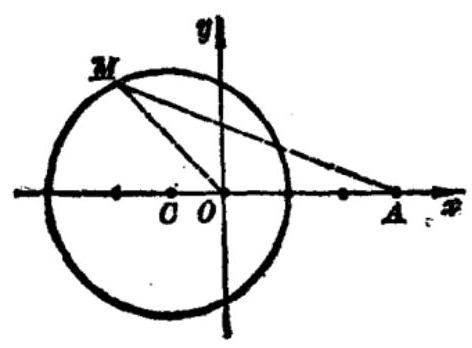
\includegraphics[max width=0.5\textwidth]{images/01912cc2-ffb6-728e-9ae7-b113ff05c64b_84_125563.jpg}
  %\documentclass[tikz, border=5pt]{standalone}
\begin{document}
	\begin{tikzpicture}[>=stealth, scale=0.6]
		% 绘制坐标轴
		\draw[->] (-3.5,0) -- (4,0) node[below ] {$x$};
		\draw[->] (0,-2.5) -- (0,3) node[below left] {$y$};
		\node at (0,0) [below left] {$O$};
		
		% 绘制圆(圆心在原点,半径设为2)
		\draw[thick] (-1,0) circle (2);
		
		% 定义切点M的坐标(M(√2, √2),在圆上且位于第一象限)
		\coordinate (A) at (3,0);
		\coordinate (C) at (-1,0);
		\coordinate (M) at (-2,{sqrt(3)});
		
		% 绘制从原点到切点M的线段(虚线)
		\draw[thick] (0,0) -- (M);
		\draw[thick] (A) -- (M);
		
		% 标记切点M
		\fill (M) circle (2pt) node[above ] {$M$}; % 圆上的点
		\fill(A) circle (2pt) node (A) [below] {$A$};
		\fill(C) circle (2pt) node (C) [below] {$C$};
		
	\end{tikzpicture}
\end{document}

  \caption{图 2-10}
\end{figure}

化简得

\[
    {x}^{2} + {y}^{2} + {2x} - 3 = 0. \tag{2}
\]

这就是所求的曲线方程.

把方程 (2) 配方, 得

\[
    {\left( x + 1\right) }^{2} + {y}^{2} = 4\text{. }
\]

所以方程 (2) 的曲线是以 \(C\left( {-1,0}\right)\) 为圆心, \(r = 2\) 为半径的圆, 它的图形如图 2-10.

\begin{problemset}[练习]

\item 下列方程各表示什么图形?

(1) \({x}^{2} + {y}^{2} = 0\) ; (2) \({x}^{2} + {y}^{2} - {2x} + {4y} - 6 = 0\) ;

(3) \({x}^{2} + {y}^{2} + {2ax} - {b}^{2} = 0\) .

\item 求下列各圆的半径和圆心坐标:

(1) \({x}^{2} + {y}^{2} - {6x} = 0\) ; (2) \({x}^{2} + {y}^{2} + {2by} = 0\) .
\end{problemset}

\begin{problemset}[习 题 五]

\item 求下列各圆的方程, 并画出它的图形:

(1) 过点 \(C\left( {-1,1}\right)\) 和 \(D\left( {1,3}\right)\) ,圆心在 \(x\) 轴上;

(2)过直线 \(x + {3y} + 7 = 0\) 与 \({3x} - {2y} - {12} = 0\) 的交点,圆心为点 \(C\left( {-1,1}\right)\) ;

(3)半径是 5,圆心在 \(y\) 轴上,且与直线 \(y = 6\) 相切;

(4)过点 \(A\left( {5,2}\right)\) 和 \(B\left( {3, - 2}\right)\) ,圆心在直线 \({2x} - y = 3\) 上.

\item 求下列条件所决定的圆的方程:

(1)圆心为 \(C\left( {3, - 5}\right)\) ,并且与直线 \(x - {7y} + 2 = 0\) 相切;

(2)过点 \(A\left( {3,2}\right)\) ,圆心在直线 \(y = {2x}\) 上,且与直线 \(y = {2x}\) +5 相切.

\item 已知: 一个圆的直径端点是 \(A\left( {{x}_{1},{y}_{1}}\right) \text{、}B\left( {{x}_{2},{y}_{2}}\right)\) . 证明: 圆的方程是 \(\left( {x - {x}_{1}}\right) \left( {x - {x}_{2}}\right) + \left( {y - {y}_{1}}\right) \left( {y - {y}_{2}}\right) = 0\) .

\item 一个等腰三角形底边上的高等于 5 , 底边两端点的坐标是 \(\left( {-4,0}\right)\) 和 \(\left( {4,0}\right)\) . 求它的外接圆的方程.

\item 赵州桥的 跨度是 37.4 米, 圆拱高约为 7.2 米. 求 这座圆拱桥的拱圆的方程.

\begin{figure}[h]
  \centering
%  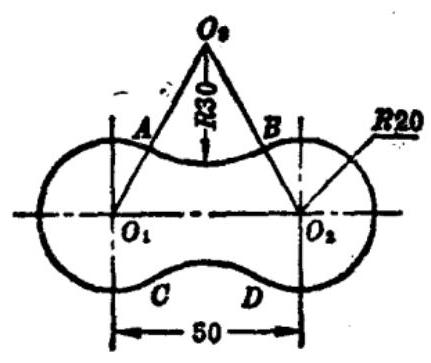
\includegraphics[max width=0.4\textwidth]{images/01912cc2-ffb6-728e-9ae7-b113ff05c64b_85_663180.jpg}
  %\documentclass[tikz, border=5pt]{standalone}
\begin{document}
	\begin{tikzpicture}[>=stealth, scale=0.8] % 箭头样式为stealth,
		
		% 绘制坐标轴
		\draw[dashed] (-5,0) -- (5,0) ; % x轴(带箭头和标签)
		\draw[dashed] (-2.5,-3) -- (-2.5,3) ; 
		\draw[dashed] (2.5,-3) -- (2.5,3) ; 
		
		\node at (2.5,0) [below right] {$O_2$};  % 原点O的标签
		\node at (-2.5,0) [below right] {$O_1$};  % 原点O的标签
		
		% 定义各关键点坐标
		% 3. 计算圆弧的起点(120°)和终点(-120°)坐标
		% 公式:圆心(x0,y0),半径r,角度θ对应的坐标为 (x0 + r·cosθ, y0 + r·sinθ)
		\coordinate (B) at (1.5, {sqrt(3)});   % 120°起点
		\coordinate (A) at (-1.5, {sqrt(3)}); % -120°终点
		\coordinate (C) at (-1.5, {-sqrt(3)});  % 点A₂
		\coordinate (D) at (1.5, {-sqrt(3)}); % 点P₂
		\coordinate (O_3) at (0,{2.5*sqrt(3)}); % 点P₂
		
		% 绘制拱形
		\draw[line width=1pt] (B) arc (120: -120:2);
		\draw[line width=1pt] (A) arc (60:300:2) ;
		
		\draw[line width=1pt] (B) arc (-60: -120:3) ;
		\draw[line width=1pt] (D) arc (60: 120:3) ;
		
		% 绘制
		\draw[thick] (2.5,0) -- (O_3) ;
		\draw[thick] (-2.5,0) -- (O_3) ;
		\draw[thick] (2.5,0) -- (4.5,2) -- (5,2) node[midway, above] {$R20$} ;
		\draw[<->] (-2.5,-2.5) -- (2.5,-2.5) node[midway] {$50$};
		\draw[->] (O_3) --++ (-90:3) node[midway] {$R30$} ;
		
		% 标记各点的标签
		\node[above] at (A) {$A$};
		\node[above] at (B) {$B$};
		\node[below] at (C) {$C$};
		\node[below] at (D) {$D$};
		\node[above] at (O_3) {$O_3$};
		
	\end{tikzpicture}
\end{document}

  \caption{(第 6 题)}
\end{figure}

\item 某工件尺寸如图所示, 它的外缘由四段圆弧连接而成. 求各段圆弧所在的圆的方程.

\item 求通过点 \(A\left( {1,2}\right)\) ,且与两坐标轴同时相切的圆的方程.

\item 过点 \(A\left( {0,\sqrt{10}}\right)\) 向圆 \({x}^{2} + {y}^{2} = 5\) 引两条切线. 求它们的方程.

\item 求下列各圆的一般方程:

(1) 过点 \(A\left( {5,1}\right)\) ,圆心在点 \(C\left( {8, - 3}\right)\) ;

(2) 过三点 \(A\left( {-1,5}\right) \text{、}B\left( {5,5}\right) \text{、}C\left( {6, - 2}\right)\) .

\item 求下列各圆的圆心坐标和半径, 并画出它们的图形:

(1) \({x}^{2} + {y}^{2} - {2x} - 5 = 0\) ; (2) \({x}^{2} + {y}^{2} + {2x} - {4y} - 4 = 0\) ;

(3) \({x}^{2} + {y}^{2} + {2ax} = 0\) ; (4) \({x}^{2} + {y}^{2} - {2by} - 2{b}^{2} = 0\) .

\item 求证: 两圆 \({x}^{2} + {y}^{2} - {4x} - {6y} + 9 = 0\) 和 \({x}^{2} + {y}^{2} + {12x} + {6y}\) \(- {19} = 0\) 相外切.

\item 求直线 \({4x} - {3y} = {50}\) 和圆 \({x}^{2} + {y}^{2} = {100}\) 的交点,说明它们的位置关系.

\item 求经过两圆 \({x}^{2} + {y}^{2} + {6x} - 4 = 0\) 和 \({x}^{2} + {y}^{2} + {6y} - {28} = 0\) 的交点,并且圆心在直线 \(x - y - 4 = 0\) 上的圆的方程.

\item 等腰三角形的顶点是 \(A\left( {4,2}\right)\) ,底边一个端点是 \(B\left( {3,5}\right)\) . 求另一个端点的轨迹方程, 并说明它的轨迹是什么.

\item 一条线段 \({AB}\left( {{AB} = {2a}}\right)\) 的两个端点 \(A\) 和 \(B\) 分别在 \(x\) 轴和 \(y\) 轴上滑动. 求线段 \({AB}\) 的中点 \(M\) 的轨迹方程.
\end{problemset}

\section*{三\text{ }椭 圆}

\section{ 椭圆及其标准方程}

椭圆是一种常见的曲线, 如汽车油罐横截面的轮廓, 天体中一些行星和卫星运行的轨道. 在立体几何中画直观图时, 圆的一种直观图也是椭圆.

取一条一定长的细绳, 把它的两端固定在画图板上的 \({F}_{1}\) 和 \({F}_{2}\) 两点 (图 2-11),当绳长大于 \({F}_{1}\) 和 \({F}_{2}\) 的距离时,用铅笔尖把绳子拉紧, 使笔尖在图板上慢慢移动, 就可以画出一个椭圆.

\begin{figure}[h]
  \centering
  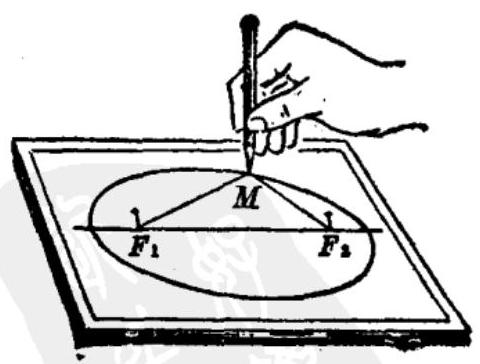
\includegraphics[max width=0.5\textwidth]{images/01912cc2-ffb6-728e-9ae7-b113ff05c64b_86_465051.jpg}
  \caption{图 2-11}
\end{figure}

从上面的画图过程,我们可以看出,椭圆是由与点 \({F}_{1}\) 和 \({F}_{2}\) 的距离的和等于这条绳长的点组成的.
\begin{definition}[椭圆] 
我们把平面内与两个定点 \({\overrightarrow{F}}_{1}\text{、}{\overrightarrow{F}}_{2}\) 的距离的和等于常数 (大于 \(\left| {{F}_{1}{F}_{2}}\right|\) ) 的点的轨迹叫做椭圆. 这两个定点叫做椭圆的焦点, 两焦点的距离叫做焦距.
\end{definition}
根据椭圆的定义, 我们来求椭圆的方程.

\begin{figure}[h]
  \centering
%  \includegraphics[max width=0.4\textwidth]{images/01912cc2-ffb6-728e-9ae7-b113ff05c64b_87_155934.jpg}
  %\documentclass[tikz, border=5pt]{standalone}
\begin{document}
	\begin{tikzpicture}[>=stealth, scale=0.6]
		% 1. 绘制坐标轴
		\draw[->] (-6,0) -- (6,0) node[below] {$x$};
		\draw[->] (0,-4) -- (0,4) node[below left] {$y$};
		\node at (0,0) [below right] {$O$};
		
		% 2. 定义椭圆参数(长半轴a=5,短半轴b=3,焦距c=4,满足a²=b²+c²)
		\def\a{5}  % 长半轴
		\def\b{3}  % 短半轴
		\def\c{4}  % 焦距(c = sqrt(a² - b²) = 4)
		
		% 3. 绘制椭圆
		\draw[thick] (0,0) ellipse ({\a} and {\b});
		
		% 4. 标记焦点F1、F2
		\fill (-{\c},0) circle (1.5pt) node[below] {$F_1$};
		\fill ({\c},0) circle (1.5pt) node[below] {$F_2$};
		
		% 5. 标记原点到焦点的距离c
		\draw[dashed] (0,0) -- ({\c},0) node[midway, below] {$c$};
		\draw[dashed] (0,0) -- (-{\c},0) node[midway, below] {$c$};
		
		% 6. 定义椭圆上点M(示例:M(3, 2.4),满足椭圆方程x²/25 + y²/9 = 1)
		\coordinate (M) at (3, 2.4);
		\fill (M) circle (1.5pt) node[above right] {$M$};
		
		% 7. 绘制线段F1M和F2M
		\draw (-{\c},0) -- (M);
		\draw ({\c},0) -- (M);
		
	\end{tikzpicture}
\end{document}

  \caption{图 2-12}
\end{figure}

取过焦点 \({F}_{1}\text{、}{F}_{2}\) 的直线为 \(x\) 轴,线段 \({F}_{1}{F}_{2}\) 的垂直平分线为 \(y\) 轴,建立直角坐标系 (图 2-12).

设 \(M\left( {x,y}\right)\) 是椭圆上任意一点,椭圆的焦距为 \({2c}\left( {c > 0}\right)\) , \(M\) 与 \({F}_{1}\) 和 \({F}_{2}\) 的距离的和等于正常数 \({2a}\) ,则 \({F}_{1}\text{、}{F}_{2}\) 的坐标分别是 \(\left( {-c,0}\right) \text{、}\left( {c,0}\right)\) .

椭圆就是集合

\[
  P = \left\{ {M\left| \right| M{F}_{1}\left| +\right| M{F}_{2} \mid = {2a}}\right\} .
\]

\[
  \because \left| {M{F}_{1}}\right| = \sqrt{{\left( x + c\right) }^{2} + {y}^{2}},\left| {M{F}_{2}}\right| = \sqrt{{\left( x - c\right) }^{2} + {y}^{2}}\text{,}
\]

得方程

\[
  \sqrt{{\left( x + c\right) }^{2} + {y}^{2}} + \sqrt{{\left( x - c\right) }^{2} + {y}^{2}} = {2a}.
\]

将这个方程移项, 两边平方, 得

\[
    {\left( x + c\right) }^{2} + {y}^{2} = 4{a}^{2} - {4a}\sqrt{{\left( x - c\right) }^{2} + {y}^{2}} + {\left( x - c\right) }^{2} + {y}^{2},
\]

\[
    {a}^{2} - {cx} = a\sqrt{{\left( x - c\right) }^{2} + {y}^{2}}.
\]

两边再平方, 得

\[
    {a}^{4} - 2{a}^{2}{cx} + {c}^{2}{x}^{2} = {a}^{2}{x}^{2} - 2{a}^{2}{cx} + {a}^{2}{c}^{2} + {a}^{2}{y}^{2},
\]

整理得

\[
  \left( {{a}^{2} - {c}^{2}}\right) {x}^{2} + {a}^{2}{y}^{2} = {a}^{2}\left( {{a}^{2} - {c}^{2}}\right) .
\]

由椭圆定义可知, \({2a} > {2c}\) ,即 \(a > c\) ,所以 \({a}^{2} - {c}^{2} > 0\) .

设 \({a}^{2} - {c}^{2} = {b}^{2}\;\left( {b > 0}\right)\) ,得

\[
    {b}^{2}{x}^{2} + {a}^{2}{y}^{2} = {a}^{2}{b}^{2}
\]

两边除以 \({a}^{2}{b}^{2}\) ,得

\begin{definition}[椭圆的标准方程] 
\[
  \frac{{x}^{2}}{{a}^{2}} + \frac{{y}^{2}}{{b}^{2}} = 1\left( {a > b > 0}\right) . \tag{1}
\]
这个方程叫 做椭圆的标准方程. 它所表示的椭圆的焦点在 \(x\) 轴上,焦点是 \({F}_{1}\left( {-c,0}\right) \text{、}{F}_{2}\left( {c,0}\right)\) ,这里 \({c}^{2} = {a}^{2} - {b}^{2}\) .
\end{definition}

\begin{corollary}[椭圆的标准方程2]
如果椭圆的焦点在 \(y\) 轴上,焦点是 \({F}_{1}(0\) , \(- c)\text{、}{F}_{2}\left( {0,c}\right)\) (图 2-13),只要将方程 (1) 的 \(x\) 、 \(y\) 互换,就可以得到它的方程. 这时方程为
\[
  \frac{{y}^{2}}{{a}^{2}} + \frac{{x}^{2}}{{b}^{2}} = 1\;\left( {a > b > 0}\right) .
\]
这个方程也是椭圆的标准方程.
\end{corollary}

\begin{figure}[h]
  \centering
%  \includegraphics[max width=0.3\textwidth]{images/01912cc2-ffb6-728e-9ae7-b113ff05c64b_88_686468.jpg}
  %\documentclass[tikz, border=5pt]{standalone}
\begin{document}
	\begin{tikzpicture}[>=stealth, scale=0.6]
		% 1. 绘制坐标轴
		\draw[->] (-4,0) -- (4,0) node[below] {$x$};
		\draw[->] (0,-6) -- (0,6) node[below left] {$y$};
		\node at (0,0) [below right] {$O$};
		
		% 2. 定义椭圆参数(长半轴a=5,短半轴b=3,焦距c=4,满足a²=b²+c²)
		\def\a{3}  % 长半轴
		\def\b{5}  % 短半轴
		\def\c{4}  % 焦距(c = sqrt(a² - b²) = 4)
		
		% 3. 绘制椭圆
		\draw[thick] (0,0) ellipse ({\a} and {\b});
		
		% 4. 标记焦点F1、F2
		\fill (0,-{\c}) circle (1.5pt) node[right] {$F_1$};
		\fill (0,{\c}) circle (1.5pt) node[right] {$F_2$};
		
		% 5. 标记原点到焦点的距离c
		\draw[dashed] (0,0) -- (0,-{\c}) node[midway, right] {$c$};
		\draw[dashed] (0,0) -- (0,{\c}) node[midway, right] {$c$};
		
		% 6. 定义椭圆上点M(示例:M(3, 2.4),满足椭圆方程x²/25 + y²/9 = 1)
		\coordinate (M) at (-2.4, -3);
		\fill (M) circle (1.5pt) node[above right] {$M$};
		
		% 7. 绘制线段F1M和F2M
		\draw (0,-{\c}) -- (M);
		\draw (0,{\c}) -- (M);
		
	\end{tikzpicture}
\end{document}

  \caption{图 2-13}
\end{figure}

例 1 平面内两个定点的距离是 8 , 写出到这两个定点的距离的和是 10 的点的轨迹的方程.

解: 这个轨迹是一个椭圆,两个定点是焦点,用 \({F}_{1}\text{、}{F}_{2}\) 表示. 取过点 \({F}_{1}\) 和 \({F}_{2}\) 的直线为 \(x\) 轴,线段 \({F}_{1}{F}_{2}\) 的垂直平分线为 \(y\) 轴.

\[
  \because \;{2a} = {10},{2c} = 8\text{,}
\]

\[
  \therefore \;a = 5,\;c = 4\text{. }
\]

\[
    {b}^{2} = {a}^{2} - {c}^{2} = {5}^{2} - {4}^{2} = 9,\;b = 3.
\]

因此, 这个椭圆的标准方程是

\[
  \frac{{x}^{2}}{{5}^{2}} + \frac{{y}^{2}}{{3}^{2}} = 1\text{,即 }\frac{{x}^{2}}{25} + \frac{{y}^{2}}{9}\;1\text{. }
\]

如果取过 \({F}_{1}\) 和 \({F}_{2}\) 的直线为 \(y\) 轴,线段 \({F}_{1}{F}_{2}\) 的垂直平分线为 \(x\) 轴,则这个椭圆的标准方程是

\[
  \frac{{y}^{2}}{25} + \frac{{x}^{2}}{9} = 1
\]

例 2 已知椭圆焦距是 \({2c}\) ,用直尺和圆规作点画出与两个焦点距离的和是 \({2a}\) 的椭圆.

画法: (1) 作线段 \({F}_{1}{F}_{2}\) ,使 \(\left| {{F}_{1}{F}_{2}}\right| = {2c}\) . 设 \({F}_{1}{F}_{2}\) 的中点为 \(O\) ,在 \({F}_{1}{F}_{2}\) 和 \({F}_{2}{F}_{1}\) 的延长线上,分别取点 \(A\text{、}{A}^{\prime }\) ; 使 \({OA}\) \(= O{A}^{\prime } = a\) (图 2-14).

\begin{figure}[h]
  \centering
%  \includegraphics[max width=0.4\textwidth]{images/01912cc2-ffb6-728e-9ae7-b113ff05c64b_89_799031.jpg}
  %\documentclass[tikz, border=5pt]{standalone}
\begin{document}
	\begin{tikzpicture}[>=stealth, scale=0.6]
		% 1. 定义椭圆参数(长半轴a=5,短半轴b=3,焦距c=4)
		\def\a{5}  % 长半轴
		\def\b{3}  % 短半轴
		\def\c{4}  % 焦距(c = sqrt(a² - b²) = 4)
		
		% 2. 绘制椭圆
		\draw[thick] (0,0) ellipse ({\a} and {\b});
		
		% 3. 绘制x轴(含标记点)
		\draw[->] (-5.5,0) -- (5.5,0);
		\fill (-5,0) circle (1pt) node[above left] {$A'$};  % 左顶点
		\fill (5,0) circle (1pt) node[above right] {$A$};   % 右顶点
		\fill (0,0) circle (1pt) node[above] {$O$};   % 原点O
		\fill (-4,0) circle (1pt) node[below] {$F_1$}; % 左焦点
		\fill (4,0) circle (1pt) node[below] {$F_2$}; % 右焦点
		
		% 4. 标记线段上的点 M1, M2
		\coordinate (M1) at (-3, 0); % 点 M1
		\coordinate (M2) at (-2, 0);   % 点 M2
		\fill (M1) circle (1pt) node[above] {$M_1$};
		\fill (M2) circle (1pt) node[below] {$M_2$};
		
		% 6. 绘制圆弧
%		\draw (-4,0) circle (2) ;
%		\draw (-4,0) circle (3) ;
		
		% 5. 标记椭圆上的点 P1, P2, P'1, P'2
		\coordinate (P1) at (-3.75, 2);   % 上半部分点 P1
		\coordinate (P2) at (-2.5, 2.6);   % 上半部分点 P2
		\coordinate (P1p) at (-3.75, -2); % 下半部分点 P'1
		\coordinate (P2p) at (-2.5, -2.6); % 下半部分点 P'2
		\fill (P1) circle (1pt) node[above left] {$P_1$};
		\fill (P2) circle (1pt) node[above left] {$P_2$};
		\fill (P1p) circle (1pt) node[below left] {$P'_1$};
		\fill (P2p) circle (1pt) node[below left] {$P'_2$};
		
	\end{tikzpicture}
\end{document}

  \caption{图 2-14}
\end{figure}

(2)在线段 \({F}_{1}{F}_{2}\) 上任取一点 \({M}_{1}\) ,分别以点 \({F}_{1}\text{、}{F}_{2}\) 为圆心, \({A}^{\prime }{M}_{1}\text{、}A{M}_{1}\) 为半径画弧,交于点 \({P}_{1}\text{、}{P}_{1}^{\prime }\) . 改变 \({M}_{1}\) 的位置, 例如 \({M}_{2},{M}_{3},\cdots\) ,用同样方法作出点 \({P}_{2}\text{、}{P}_{2}^{\prime }\text{、}{P}_{3}\text{、}{P}_{3}^{\prime },\cdots\) .

(3)把 \({A}^{\prime }\text{、}{P}_{1}\text{、}{P}_{2}\text{、}\cdots \text{、}A\text{、}\cdots \text{、}{P}_{2}^{\prime }\text{、}{P}_{1}^{\prime }\text{、}{A}^{\prime }\) 顺次连成光滑曲线, 就得到所求的椭圆.

\begin{problemset}[练习]

\item 说明例 2 中椭圆画法的依据.

\item 写出适合下列条件的椭圆的标准方程:

(1) \(a = 4,b = 1\) ,焦点在 \(x\) 轴上;

(2) \(a = 4,c = \sqrt{15}\) ,焦点在 \(y\) 轴上;

(3)两个焦点的坐标是 \(\left( {-2,0}\right)\) 和 \(\left( {2,0}\right)\) ,并且经过点

\[
  P\left( {\frac{5}{2}, - \frac{3}{2}}\right)
\]

\item 已知 \(\bigtriangleup {ABC}\) 的一边 \({BC}\) 长为 6,周长为 16 . 求顶点 \(A\) 的

\end{problemset}

\section*{轨迹方程}

\section{椭圆的几何性质}

我们根据椭圆的标准方程

\[
  \frac{{x}^{2}}{{a}^{2}} + \frac{{y}^{2}}{{b}^{2}} = 1\;\left( {a > b > 0}\right) ,
\]

来研究椭圆的几何性质.

\section*{1. 范围}

由标准方程可知,椭圆上点的坐标 \(\left( {x,y}\right)\) 都适合不等式

\[
  \frac{{x}^{2}}{{a}^{2}} \leq 1,\;\frac{{y}^{2}}{{b}^{2}} \leq 1,
\]

\begin{figure}[h]
  \centering
%  \includegraphics[max width=0.5\textwidth]{images/01912cc2-ffb6-728e-9ae7-b113ff05c64b_90_426128.jpg}
  %\documentclass[tikz, border=5pt]{standalone}
\begin{document}
	\begin{tikzpicture}[>=stealth, scale=0.6]
		% 1. 定义椭圆参数(长半轴a=5,短半轴b=3,焦距c=4,满足c=√(a²-b²))
		\def\a{5}  % 长半轴
		\def\b{3}  % 短半轴
		\def\c{4} % 焦距(近似√(5²-3²)=√16≈4)
		
		% 2. 绘制辅助矩形(虚线)
		\draw[dashed] (-\a, -\b) rectangle (\a, \b);
		
		% 3. 绘制椭圆
		\draw[thick] (0,0) ellipse ({\a} and {\b});
		
		% 4. 绘制坐标轴
		\draw[->] (-\a-1,0) -- (\a+1,0) node[below left] {$x$};
		\draw[->] (0,-\b-1) -- (0,\b+1) node[below left] {$y$};
		\node at (0,0) [below left] {$O$}; % 原点
		
		% 5. 标记顶点与焦点
		\node at (-\a,0) [above left] {$A_1$};   % 左顶点
		\node at (\a,0)  [above right] {$A_2$};  % 右顶点
		\node at (0,\b)  [above right] {$B_2$};  % 上顶点
		\node at (0,-\b) [below right] {$B_1$};  % 下顶点
		\fill (-\c,0) circle (1pt) node[below] {$F_1$}; % 左焦点
		\fill (\c,0) circle (1pt) node[below] {$F_2$}; % 右焦点
		
		% 6. 绘制线段 B2F2
		\draw (0,\b) -- (\c,0);
		
		% 7. 标记线段长度(a, b, c)
		\node at (2,1.5) [above] {$a$};  % 线段 B2F2 标注为 a
		\node at (0,1.5) [left] {$b$};  % 从 O 到 B2 标注为 b
		\node at (2,0) [below] {$c$}; % 从 O 到 F2 标注为 c
	\end{tikzpicture}
\end{document}

  \caption{图 2-15}
\end{figure}

即 \(\;{x}^{2} \leq {a}^{2},\;{y}^{2} \leq {b}^{2}\) ,

\[
  \therefore \left| x\right| \leq a,\;\left| y\right| \leq b\text{.}
\]

这说明椭圆位于直线 \(x = \pm a\) 和 \(y = \pm b\) 所围成的矩形里 (图 2-15).

\section*{2. 对称性}

在标准方程中,把 \(x\) 换成 \(- x\) ; 或把 \(y\) 换成 \(- y\) ; 或把 \(x\text{、}y\) 同时换成 \(- x\text{、} - y\) 时,方程都不变. 所以图形关于 \(y\) 轴、 \(x\) 轴和原点都是对称的. 这时, 坐标轴是椭圆的对称轴, 原点是椭圆的对称中心. 椭圆的对称中心叫做椭圆的中心.

\section*{3. 顶点}

在标准方程中,令 \(x = 0\) ,得 \(y = \pm b\) . 这说明 \({B}_{1}\left( {0, - b}\right)\) 、 \({B}_{2}\left( {0,b}\right)\) 是椭圆和 \(y\) 轴的两个交点. 同理,令 \(y = 0\) 时,得 \(x\) \(= \pm a,{A}_{1}\left( {-a,0}\right) \text{、}{A}_{2}\left( {a,0}\right)\) 是椭圆和 \(x\) 轴的两个交点. 因为 \(x\) 轴、 \(y\) 轴是椭圆的对称轴,所以椭圆和它的对称轴有四个交点, 这四个交点, 叫做椭圆的顶点.

线段 \({A}_{1}{A}_{2}\text{、}{B}_{1}{B}_{2}\) 分别叫做椭圆的长轴和短轴. 它们的长分别等于 \({2a}\) 和 \({2b},a\) 和 \(b\) 分别叫做椭圆的长半轴长和短半轴长.

\section*{4. 离心率}

椭圆的焦距与长轴长的比 \(e = \frac{c}{a}\) ,叫做椭圆的离心率.

因为 \(a > c > 0\) ,所以 \(0 < e < 1.e\) 越接近 1,则 \(c\) 越接近 \(a\) , 从而 \(b = \sqrt{{a}^{2} - {c}^{2}}\) 越小,因此椭圆越扁; 反之, \(e\) 越接近于 \(0,c\) 越接近于 0,从而 \(b\) 越接近于 \(a\) ,这时椭圆就接近于圆.

如果 \(a = b\) ,则 \(c = 0\) ,两个焦点重合,这时椭圆的标准方程成为

\[
    {x}^{2} + {y}^{2} = {a}^{2}
\]

图形就是圆了.

例 1 求椭圆 \({16}{x}^{2} + {25}{y}^{2} = {400}\) 的长轴和短轴的长、离心率、焦点和顶点的坐标, 并用描点法画出它的图形.

解: 把已知方程化成标准方程

\[
  \frac{{x}^{2}}{{5}^{2}} + \frac{{y}^{2}}{{4}^{2}} = 1
\]

这里, \(a = 5,b = 4,c = \sqrt{{25} - {16}} = 3\) .

因此,椭圆的长轴和短轴的长分别是 \({2a} = {10}\) 和 \({2b} = 8\) , 离心率 \(e = \frac{c}{a} = \frac{3}{5} = {0.6}\) ,两个焦点分别是 \({F}_{1}\left( {-3,0}\right)\) 和 \({F}_{2}(3\) , \(0)\) ,椭圆的四个顶点是 \({A}_{1}\left( {-5,0}\right) \text{、}{A}_{2}\left( {5,0}\right) \text{、}{B}_{1}\left( {0, - 4}\right)\) 和 \({B}_{2}\left( {0,4}\right)\) .

将已知方程变形为 \(y = \pm \frac{4}{5}\sqrt{{25} - {x}^{2}}\) . 根据

\[
  y = + \frac{4}{5}\sqrt{{25} - {x}^{2}}
\]

在第一象限 \(x \leq 5\) 的范围内算出几个点的坐标 \(\left( {x,y}\right)\) :

\begin{center}
	\adjustbox{max width=\textwidth}{
		\begin{tabular}{|c|c|c|c|c|c|c|}
			\hline
			x & 0 & 1 & 2 & 3 & 4 & 5 \\
			\hline
			y & 4 & 3.9 & 3.7 & 3.2 & 2.4 & 0 \\
			\hline
		\end{tabular}
	}
\end{center}

先描点画出椭圆在第一象限内的图形, 再利用椭圆的对称性就画出整个椭圆(图 2-16).

\begin{figure}[h]
	\centering
	% 左侧图片:宽度设置为0.45倍文本宽度,预留间距
	\begin{subfigure}[h]{0.45\textwidth}
		\centering
		%  \includegraphics[max width=0.4\textwidth]{images/01912cc2-ffb6-728e-9ae7-b113ff05c64b_92_523518.jpg}
		%\documentclass[tikz, border=5pt]{standalone}
\begin{document}
	\begin{tikzpicture}[>=stealth, scale=0.6]
		% 1. 定义椭圆参数(长半轴a=5,短半轴b=4,焦距c=3,满足c=√(a²-b²))
		\def\a{5}  % 长半轴
		\def\b{4}  % 短半轴
		\def\c{3} % 焦距(近似√(5²-3²)=√16≈4)
		
		% 2. 绘制辅助矩形(虚线)
		\draw[dashed] (-\a, -\b) rectangle (\a, \b);
		
		% 3. 绘制椭圆
		\draw[thick] (0,0) ellipse ({\a} and {\b});
		
		% 4. 绘制坐标轴
		\draw[->] (-\a-1,0) -- (\a+1,0) node[below left] {$x$};
		\draw[->] (0,-\b-1) -- (0,\b+1) node[below left] {$y$};
		\node at (0,0) [below left] {$O$}; % 原点
		
		% 绘制所有小刻度线(从 -1 到 2,每隔 1 单位画竖线)
		\foreach \x in {-4,-3,...,4} {
			\draw (\x, 0.1) -- (\x, -0.1) ;  % 小竖线(长 0.2 单位)
		}
		\foreach \y in {-3,-2,...,3} {
			\draw (0.1,\y) -- (-0.1,\y) ;  % 小竖线(长 0.2 单位)
		}
		
		% 5. 标记顶点与焦点
		\node at (-\a,0) [above left] {$A_1$};   % 左顶点
		\node at (\a,0)  [above right] {$A_2$};  % 右顶点
		\node at (0,\b)  [above right] {$B_2$};  % 上顶点
		\node at (0,-\b) [below right] {$B_1$};  % 下顶点
		\fill (-\c,0) circle (1pt) node[below] {$F_1$}; % 左焦点
		\fill (\c,0) circle (1pt) node[below] {$F_2$}; % 右焦点
		
		% 6. 绘制
		\fill (1,3.92) circle(2pt);
		\fill (2,3.66) circle(2pt);
		\fill (3,3.2) circle(2pt);
		\fill (4,2.4) circle(2pt);
		
	\end{tikzpicture}
\end{document}

		\caption{图 2-16}
	\end{subfigure}
	\hfill % 两个图片之间添加空白填充,确保左右分布
	% 右侧图片:宽度设置为0.45倍文本宽度
	\begin{subfigure}[h]{0.45\textwidth}
		\centering
		%  \includegraphics[max width=0.4\textwidth]{images/01912cc2-ffb6-728e-9ae7-b113ff05c64b_92_511935.jpg}
		%\documentclass[tikz, border=5pt]{standalone}
\begin{document}
	\begin{tikzpicture}[>=stealth, scale=0.6]
		% 3. 绘制椭圆
		\draw[thick] (0.5,0) circle(3);
		\draw[thick] (0,0) ellipse ({3.8} and {3.7});
		
		% 4. 绘制坐标轴
		\draw[->] (-4.5,0) -- (5,0) node[below left] {$x$};
		\draw[->] (0,-4.5) -- (0,4.5) node[below left] {$y$};
		\node at (0,0) [below left] {$O$}; % 原点
		
		% 5. 标记顶点与焦点
		\node at (-3.8,0) [below left] {$B$};   % 左顶点
		\node at (3.8,0)  [above right] {$A$};  % 右顶点
		\fill (-0.5,0) circle (2pt) node[above] {$F_1$}; % 左焦点
		\fill (0.5,0) circle (2pt) node[above] {$F_2$}; % 右焦点
		
	\end{tikzpicture}
\end{document}

		\caption{图 2-17}
	\end{subfigure}
	%  \caption{}
\end{figure}

例2 我国发射的第一颗人造地球卫星的运行轨道, 是以地球的中心为一个焦点的椭圆,近地点 \(A\) 距地面 439 公里,远地点 \(B\) 距地面 2384 公里,地球半径约为 6371 公里. 求卫星的轨道方程.

解: 选取坐标系如图 2-17.

\[
  a - c = \left| {OA}\right| - \left| {O{F}_{2}}\right| = \left| {{F}_{2}A}\right| = {6371} + {439} = {6810},
\]

\[
  a + c = \left| {OB}\right| + \left| {O{F}_{2}}\right| = \left| {{F}_{2}B}\right| = {6371} + {2384} = {8755}.
\]

解得

\[
  a = {7782.5},c = {972.5}\text{. }
\]

\(\therefore b = \sqrt{{a}^{2} - {c}^{2}} = \sqrt{\left( {a + c}\right) \left( {a - c}\right) } = \sqrt{{8755} \times {6810}}\)

\[
  = {7721.5}\text{.}
\]

因此, 卫星的轨道方程 (近似) 是

\[
  \frac{{x}^{2}}{{7783}^{2}} + \frac{{y}^{2}}{{7722}^{2}} = 1
\]

例 3 点 \(M\left( {x,y}\right)\) 与定点 \(F\left( {c,0}\right)\) 的距离和它到定直线 \(l\) : \(x = \frac{{a}^{2}}{c}\) 的距离的比是常数 \(\frac{c}{a}\left( {a > c > 0}\right)\) . 求点 \(M\) 的轨迹 (图 2-18).

解: 设 \(d\) 是点 \(M\) 到直线 \(l\) 的距离. 根据题意,所求轨迹就是集合

\[
  P = \left\{ {M\left| {\;\frac{\left| MF\right| }{d} = \frac{c}{a}}\right. }\right\}
\]

\begin{figure}[h]
  \centering
  \includegraphics[max width=0.5\textwidth]{images/01912cc2-ffb6-728e-9ae7-b113ff05c64b_93_181051.jpg}
  \caption{图 2-18}
\end{figure}

由此得

\[
  \frac{\sqrt{{\left( x - c\right) }^{2} + {y}^{2}}}{\left| \frac{{a}^{2}}{c} - x\right| } = \frac{c}{a}
\]

将上式化简, 得

\[
  \left( {{a}^{2} - {c}^{2}}\right) {x}^{2} + {a}^{2}{y}^{2} = {a}^{2}\left( {{a}^{2} - {c}^{2}}\right) .
\]

设 \({a}^{2} - {c}^{2} = {b}^{2}\) ,就可化成

\[
  \frac{{x}^{2}}{{a}^{2}} + \frac{{y}^{2}}{{b}^{2}} = 1
\]

这是椭圆的标准方程,所以点 \(M\) 的轨迹是椭圆.

由上面的例子可知,点 \(M\) 与一个定点的距离和它到一条定直线的距离的比是常数 \(e = \frac{c}{a}\left( {e < 1}\right)\) 时,这个点的轨迹是椭圆. 定点是椭圆的焦点,定直线叫做椭圆的准线,常数 \(e\) 是椭圆的离心率.

对于椭圆 \(\frac{{x}^{2}}{{a}^{2}} + \frac{{y}^{2}}{{b}^{2}} = 1\) ,相应于焦点 \(F\left( {c,0}\right)\) 的准线方程是 \(x = \frac{{a}^{2}}{c}\) . 根据椭圆的对称性,相应于焦点 \({F}^{\prime }\left( {-c,0}\right)\) 的准线方程是 \(x = - \frac{{a}^{2}}{c}\) ,所以椭圆有两条准线.

\begin{problemset}[练习]

\item 说出椭圆 \(\frac{{y}^{2}}{{a}^{2}} + \frac{{x}^{2}}{{b}^{2}} = 1\) 的焦点和顶点的坐标.

\item 求下列各椭圆的长轴和短轴的长、离心率、焦点坐标、顶点坐标和准线方程, 并画出草图:

(1) \(\frac{{x}^{2}}{25} + \frac{{y}^{2}}{9} = 1\) ; (2) \(9{x}^{2} + {y}^{2} = {81}\) ;

(3) \({x}^{2} + 4{y}^{2} = {16}\) ; (4) \(2{x}^{2} = 1 - {y}^{2}\) .

\item 求适合下列条件的椭圆的标准方程:

(1) \(a = 6,e = \frac{1}{3}\) ,焦点在 \(x\) 轴上;

(2) \(c = 3,e = \frac{3}{5}\) ,焦点在 \(y\) 轴上.

\end{problemset}

\begin{problemset}[习 题 六]

\item 如图,椭圆上的点中, \({A}_{1}\) 与焦点 \({F}_{1}\) 的距离最小, \(\left| {{A}_{1}{F}_{1}}\right|\) \(= 2,{A}_{2}\) 与 \({F}_{1}\) 的距离最大, \(\left| {{A}_{2}{F}_{1}}\right| = {14}\) ,求椭圆的标准方程。

\begin{figure}[h]
	\centering
	\includegraphics[max width=0.4\textwidth]{images/01912cc2-ffb6-728e-9ae7-b113ff05c64b_94_706053.jpg}
	\caption{(第 1 题)}
\end{figure}

\item 已知椭圆的面积公式是 \(S = {\pi ab}\) ,其中 \(a\text{、}b\) 分别是椭圆长半轴和短半轴的长. 利用这个公式, 求下列椭圆的面积:

(1) \(9{x}^{2} + {y}^{2} = 8\) ; (2) \(9{x}^{2} + {25}{y}^{2} = {100}\) .

\item 求椭圆 \(\frac{{x}^{2}}{16} + \frac{{y}^{2}}{25} = 1\) 上一点 \({M}_{1}\left( {{2.4},4}\right)\) 与焦点的距离.

\item 求适合下列条件的椭圆的标准方程:

(1)椭圆经过两点 \(P\left( {-2\sqrt{2},0}\right) \text{、}Q\left( {0,\sqrt{5}}\right)\) ;

(2) 长轴是短轴的 3 倍,椭圆经过点 \(P\left( {3,0}\right)\) ;

(3) 焦点坐标是 \(\left( {-2\sqrt{3},0}\right)\) 和 \(\left( {2\sqrt{3},0}\right)\) ,并且经过点

\[
  P\left( {\sqrt{5}, - \sqrt{6}}\right)
\]

(4)离心率等于 0.8 , 焦距是 8 .

\item 讨论下列椭圆的范围, 并描点画出图形:

(1) \(4{x}^{2} + {y}^{2} = {16}\) ; (2) \(5{x}^{2} + 9{y}^{2} = {100}\) ;

(3) \(2{x}^{2} = 1 - {y}^{2}\) .

\item 我国发射的科学实验人造地球卫星的运行轨道是以地球的中心为一个焦点的椭圆, 近地点距地面 266 公里, 远地点距地面 1826 公里. 求这颗卫星的轨道方程.

\item 彗星“紫金山一号”是南京天文台发现的. 它的运行轨道是以太阳为一个焦点的椭圆. 测得轨道的近日点距太阳中心 1.486 天文单位, 远日点距太阳中心 5.563 天文单位 (1 天文单位是太阳到地球的平均距离, 约 1.5 亿公里), 求椭圆的方程.

\item 已知地球运行的轨道是长半轴长 \(a = {1.50} \times {10}^{8}\mathrm{\;{km}}\) ,离心率 \(e = {0.0192}\) 的椭圆. 太阳在这个椭圆的一个焦点上. 求地球到太阳最大和最小的距离.

\item 求下列椭圆的离心率:

(1)从焦点看短轴两端点的视角为 \({60}^{ \circ }\) ;

(2)从短轴的一个端点看两焦点的视角为直角.

\item 点 \(P\) 与一定点 \(F\left( {2,0}\right)\) 的距离和它到一定直线 \(x = 8\) 的距离的比是 1:2. 求点 \(P\) 的轨迹方程,并说明轨迹是什么图形.

\item \(\bigtriangleup {ABC}\) 的一边的两顶点是 \(B\left( {0,6}\right)\) 和 \(C\left( {0, - 6}\right)\) ,另两边的斜率的乘积是 \(- \frac{4}{9}\) ,求顶点 \(A\) 的轨迹.

\item 点 \(M\) 与椭圆 \(\frac{{x}^{2}}{{13}^{2}} + \frac{{y}^{2}}{{12}^{2}} = 1\) 的左焦点和右焦点的距离的比为 2:3. 求点 \(M\) 的轨迹方程,并画出图形.

\item 已知直线和椭圆的方程如下, 求它们的交点坐标:

(1) \({3x} + {10y} - {25} = 0,\frac{{x}^{2}}{25} + \frac{{y}^{2}}{4} = 1\) ;

(2) \({3x} - y + 2 = 0,\frac{{x}^{2}}{16} + \frac{{y}^{2}}{4} = 1\) .

\item 求证两椭圆 \({b}^{2}{x}^{2} + {a}^{2}{y}^{2} - {a}^{2}{b}^{2} = 0,{a}^{2}{x}^{2} + {b}^{2}{y}^{2} - {a}^{2}{b}^{2} = 0\) 的交点在以原点为中心的圆周上, 并求这个圆的方程.

\end{problemset}

\section*{四\text{ }双曲线}

\section{双曲线及其标准方程}

我们知道, 与两定点的距离的和为常数的点的轨迹是椭圆, 那么与两定点的距离的差为常数的点的轨迹又是怎样的曲线: 这就是我们下面要讨论的问题.
\begin{definition}[双曲线] 
平面内与两个定点 \({F}_{1}\text{、}{F}_{2}\) 的距离的差的绝对值是常数 (小于 \(\left| {{F}_{1}{F}_{2}}\right|\) ) 的点的轨迹叫做双曲线. 这两个定点叫做双曲线的焦点, 两焦点的距离叫做焦距.
\end{definition}

\begin{figure}[h]
  \centering
  \includegraphics[max width=0.4\textwidth]{images/01912cc2-ffb6-728e-9ae7-b113ff05c64b_97_983208.jpg}
  \caption{图 2-19}
\end{figure}

取过焦点 \({F}_{1}\text{、}{F}_{2}\) 的直线为 \(x\) 轴,线段 \({F}_{1}{F}_{2}\) 的垂直平分线为 \(y\) 轴 (图 2-19).

设 \(M\left( {x,y}\right)\) 是双曲线上的任意一点,双曲线的焦距是 \({2c}\) \(\left( {c > 0}\right)\) ,那么, \({F}_{1}\text{、}{F}_{2}\) 的坐标分别是 \(\left( {-c,0}\right) \text{、}\left( {c,0}\right)\) . 又设点 \(M\) 与 \({F}_{1}\) 和 \({F}_{2}\) 的距离的差的绝对值等于常数 \({2a}\) .

由定义可知, 双曲线就是集合

\[
  P = \left\{ {M\left| \right| M{F}_{1}\left| -\right| M{F}_{2} \mid = \pm {2a}}\right\} ,
\]

\[
  \because \left| {M{F}_{1}}\right| = \sqrt{{\left( x + c\right) }^{2} + {y}^{2}},\left| {M{F}_{2}}\right| = \sqrt{{\left( x - c\right) }^{2} + {y}^{2}}\text{,}
\]

得方程

\[
  \sqrt{{\left( x + c\right) }^{2} + {y}^{2}} - \sqrt{{\left( x - c\right) }^{2} + {y}^{2}} = \pm {2a}.
\]

化简, 得

\[
  \left( {{c}^{2} - {a}^{2}}\right) {x}^{2} - {a}^{2}{y}^{2} = {a}^{2}\left( {{c}^{2} - {a}^{2}}\right) .
\]

由双曲线的定义, \({2c} > {2a}\) ,即 \(c > a\) ,所以 \({c}^{2} - {a}^{2} > 0\) ,设 \({c}^{2} - {a}^{2} = {b}^{2}\left( {b > 0}\right)\) ,代入上式得

\[
    {b}^{2}{x}^{2} - {a}^{2}{y}^{2} = {a}^{2}{b}^{2}
\]

也就是
\begin{definition}[双曲线的标准方程] 
\[
  \frac{{x}^{2}}{{a}^{2}} - \frac{{y}^{2}}{{b}^{2}} = 1 \tag{1}
\]

这个方程叫做双曲线的标准方程, 它所表示的双曲线的焦点在 \(x\) 轴上,焦点是 \({F}_{1}\left( {-c,0}\right) \text{、}{F}_{2}\left( {c,0}\right)\) ,这里 \({c}^{2} = {a}^{2} + {b}^{2}\) .
\end{definition}

\begin{corollary}[双曲线标准方程2]
	

如果双曲线的焦点在 \(y\) 轴上 (图 2-20),焦点是 \({F}_{1}(0\) , \(- c)\text{、}{F}_{2}\left( {0,c}\right)\) ,只要将方程 (1) 的 \(x\text{、}y\) 互换就可以得到它的方程

\[
  \frac{{y}^{2}}{{a}^{2}} - \frac{{x}^{2}}{{b}^{2}} = 1
\]

这个方程也是双曲线的标准方程.

\end{corollary}
\begin{figure}[h]
  \centering
  \includegraphics[max width=0.3\textwidth]{images/01912cc2-ffb6-728e-9ae7-b113ff05c64b_98_269004.jpg}
  \caption{图 2-20}
\end{figure}

例 已知两点 \({F}_{1}\left( {-5,0}\right) \text{、}{F}_{2}\left( {5,0}\right)\) ,求与它们的距离的差的绝对值是 6 的点的轨迹方程.

解: 按定义,所求点的轨迹是双曲线,因 \(c = 5,a = 3\) ,所以

\[
    {b}^{2} = {c}^{2} - {a}^{2} = {5}^{2} - {3}^{2} = {4}^{2},
\]

因此所求方程是

\[
  \frac{{x}^{2}}{{3}^{2}} - \frac{{y}^{2}}{{4}^{2}} = 1\text{,即 }\frac{{x}^{2}}{9} - \frac{{y}^{2}}{16} = 1\text{. }
\]

\begin{problemset}[练习]

\item 求适合下列条件的双曲线的标准方程:

(1) \(a = 4,b = 3\) ,焦点在 \(x\) 轴上;

(2) \(a = 2\sqrt{5}\) ,经过点 \(A\left( {2, - 5}\right)\) ,焦点在 \(y\) 轴上.

\item 证明: 椭圆 \(\frac{{x}^{2}}{25} + \frac{{y}^{2}}{9} = 1\) 与双曲线 \({x}^{2} - {15}{y}^{2} = {15}\) 的焦点相同。

\end{problemset}

\section{双曲线的几何性质}

我们根据双曲线的标准方程

\[
  \frac{{x}^{2}}{{a}^{2}} - \frac{{y}^{2}}{{b}^{2}} = 1
\]

来研究它的几何性质.

\section*{1. 范围}

由标准方程可知,双曲线上点的坐标 \(\left( {x,y}\right)\) ,对于任何实数 \(x,y\) 都适合不等式 \(\frac{{x}^{2}}{{a}^{2}} \geq 1\) ,即 \({x}^{2} \geq {a}^{2}\) .

\(\therefore \;x \geq a\) 或 \(x \leq - a\) .

这说明双曲线在两条直线 \(x = a,x = - a\) 的外侧.

\section*{2. 对称性}

双曲线关于每个坐标轴和原点都是对称的. 这时, 坐标轴是双曲线的对称轴, 原点是双曲线的对称中心. 双曲线的对称中心叫做双曲线的中心.

\section*{3. 顶点}

在标准方程中,令 \(y = 0\) ,得 \(x = \pm a\) ,因此双曲线和 \(x\) 轴有两个交点 \({A}_{1}\left( {-a,0}\right) \text{、}{A}_{2}\left( {a,0}\right)\) . 因为 \(x\) 轴是双曲线的对称轴, 所以双曲线和它的对称轴有两个交点, 它们叫做双曲线的顶点.

\begin{figure}[h]
  \centering
  \includegraphics[max width=0.3\textwidth]{images/01912cc2-ffb6-728e-9ae7-b113ff05c64b_99_697647.jpg}
  \caption{图 2-21}
\end{figure}

令 \(x = 0\) ,得 \({y}^{2} = - {b}^{2}\) ,这个方程没有实数根, 说明双曲线和 \(y\) 轴没有交点,但我们也把 \({B}_{1}\left( {0, - b}\right) \text{、}{B}_{2}\left( {0,b}\right)\) 画在 \(y\) 轴上(图 2-21).

线段 \({A}_{1}{A}_{2}\) 叫做双曲线的实轴,它的长等于 \({2a},a\) 叫做双曲线的实半轴长. 线段 \({B}_{1}{B}_{2}\) 叫做双曲线的虚轴,它的长等于 \({2b},b\) 叫做双曲线的虚半轴长.

\section*{4. 渐近线}

经过 \({A}_{2}\text{、}{A}_{1}\) 作 \(y\) 轴的平行线 \(x = \pm a\) ,经过 \({B}_{2}\text{、}{B}_{1}\) 作 \(x\) 轴的平行线 \(y = \pm b\) ,四条直线围成一个矩形(图 2-22). 矩形的两条对角线所在直线的方程是 \(y = \pm \frac{b}{a}x\) ,从图 2-22 可以看出,双曲线 \(\frac{{x}^{2}}{{a}^{2}} - \frac{{y}^{2}}{{b}^{2}} = 1\) 的各 支向外延伸时, 与这两条直线逐渐接近.

\begin{figure}[h]
  \centering
  \includegraphics[max width=0.3\textwidth]{images/01912cc2-ffb6-728e-9ae7-b113ff05c64b_100_513224.jpg}
  \caption{图 2-22}
\end{figure}

下面, 我们来证明这个事实.

双曲线在第一象限内的一部分的方程可写为

\[
  y = \frac{b}{a}\sqrt{{x}^{2} - {a}^{2}}\;\left( {x > a}\right) ,
\]

设 \(M\left( {x,y}\right)\) 是它上面的点, \(N\left( {x,Y}\right)\) 是直线 \(y = \frac{b}{a}x\) 上与 \(M\) 有相同横坐标的点,则 \(Y = \frac{b}{a}x\) .

\[
  \because y = \frac{b}{a}\sqrt{{x}^{2} - {a}^{2}} = \frac{b}{a}x\sqrt{1 - {\left( \frac{a}{x}\right) }^{2}} < \frac{b}{a}x = Y,
\]

\[
  \therefore \;\left| {MN}\right| = Y - y = \frac{b}{a}\left( {x - \sqrt{{x}^{2} - {a}^{2}}}\right)
\]

\[
  = \frac{b}{a} \cdot \frac{\left( {x - \sqrt{{x}^{2} - {a}^{2}}}\right) \left( {x + \sqrt{{x}^{2} - {a}^{2}}}\right) }{x + \sqrt{{x}^{2} - {a}^{2}}}
\]

\[
  = \frac{ab}{x + \sqrt{{x}^{2} - {a}^{2}}}.
\]

设 \(\left| {MQ}\right|\) 是点 \(M\) 到直线 \(y = \frac{b}{a}x\) 的距离,则 \(\left| {MQ}\right|\) \(< \left| {MN}\right|\) . 当 \(x\) 逐渐增大时, \(\left| {MN}\right|\) 逐渐减小, \(x\) 无限增大, \(\left| {MN}\right|\) 接近于零, \(\left| {MQ}\right|\) 也接近于零,就是说,双曲线在第一象限的部分从射线 \({ON}\) 的下方逐渐接近于射线 \({ON}\) .

在其他象限内也可以证明类似的情况. 我们把两条直线 \(y = \pm \frac{b}{a}x\) 叫做双曲线的渐近线. 在方程 \(\frac{{x}^{2}}{{a}^{2}} - \frac{{y}^{2}}{{b}^{2}} = 1\) 中,如果 \(a = b\) ,那么双曲线方程为 \({x}^{2} - {y}^{2} = {a}^{2}\) ,它的实轴和虚轴的长都等于 \({2a}\) . 这时,四条直线 \(x = \pm a,y = \pm a\) 围成正方形, 渐近线方程成为 \(x = \pm y\) ,它们互相垂直,并且平分双曲线实轴和虚轴所成的角. 实轴和虚轴等长的双曲线叫做等轴双曲线.

\section*{5. 离心率}

双曲线的焦距与实轴的比 \(e = \frac{c}{a}\) ,叫做双曲线的离心率. 因为 \(c > a\) ,所以双曲线的离心率 \(e > 1\) .

由等式 \({c}^{2} - {a}^{2} = {b}^{2}\) 可得

\[
  \frac{b}{a} = \frac{\sqrt{{c}^{2} - {a}^{2}}}{a} = \sqrt{\frac{{c}^{2}}{{a}^{2}} - 1} = \sqrt{{e}^{2} - 1}.
\]

因此 \(e\) 越大, \(\frac{b}{a}\) 也越大,即渐近线 \(y = \pm \frac{b}{a}x\) 的斜率的绝对值越大, 这时双曲线的形状就从扁狭逐渐变得开阔. 由此可知, 双曲线的离心率越大, 它的开口就越开阔.

例 1 求双曲线 \(9{y}^{2} - {16}{x}^{2} = {144}\) 的实半轴长和虚半轴长、焦点坐标、离心率、渐近线方程.

解: 把方程化为标准方程

\[
  \frac{{y}^{2}}{{4}^{2}} - \frac{{x}^{2}}{{3}^{2}} = 1
\]

由此可知,实半轴长 \(a = 4\) ,虚半轴长 \(b = 3\) .

\[
  c = \sqrt{{a}^{2} + {b}^{2}} = \sqrt{{4}^{2} + {3}^{2}} = 5.
\]

焦点的坐标是 \(\left( {0, - 5}\right) ,\left( {0,5}\right)\) .

离心率 \(e = \frac{c}{a} = \frac{5}{4}\) .

渐近线方程为

\[
  x = \pm \frac{3}{4}y\text{,即 }y = \pm \frac{4}{3}x\text{. }
\]

例 2 双曲线型自然通风塔的外形, 是双曲线的一部分绕其虚轴旋转所成的曲面 (图 2-23), 它的最小半径为 12 米, 上口半径为 13 米, 下口半径为 25 米, 高 55 米. 在所给的坐标系中求此双曲线的方程.

\begin{figure}[h]
  \centering
  \includegraphics[max width=0.7\textwidth]{images/01912cc2-ffb6-728e-9ae7-b113ff05c64b_102_919231.jpg}
  \caption{图 2-23}
\end{figure}

解: 在图 2-23 的坐标系中, 双曲线有标准方程

\[
  \frac{{x}^{2}}{{a}^{2}} - \frac{{y}^{2}}{{b}^{2}} = 1
\]

点 \(A\) 旋转所成的圆半径最小, \(a = {12}\) . 下面求 \(b\) .

设 \(B\) 是双曲线上位于通风塔下口的一点,它的坐标为 \(\left( {{25},{y}_{1}}\right) ;C\) 是双曲线上位于通风塔上口的一点,它的坐标为 \(\left( {{13},{y}_{2}}\right)\) . 因为 \(B\text{、}C\) 在双曲线上,所以

\[
  \frac{{25}^{2}}{{12}^{2}} - \frac{{y}_{1}^{2}}{{b}^{2}} = 1
\]

\[
  \frac{{13}^{2}}{{12}^{2}} - \frac{{y}_{2}^{2}}{{b}^{2}} = 1
\]

解得

\[
    {y}_{1} = - \frac{b}{12}\sqrt{{25}^{2} - {12}^{2}} = - \frac{b}{12}\sqrt{481}
\]

\[
    {y}_{2} = \frac{b}{12}\sqrt{{13}^{2} - {12}^{2}} = \frac{5}{12}b.
\]

因为塔高 55 米,所以 \({y}_{2} - {y}_{1} = {55}\) . 即

\[
  \frac{5}{12} + \frac{b\sqrt{481}}{12} = {55}
\]

解得

\[
  b \approx {24.5}\text{ (米). }
\]

所以双曲线方程 (近似) 为

\[
  \frac{{x}^{2}}{{12}^{2}} - \frac{{y}^{2}}{{24.5}^{2}} = 1
\]

例 3 以已知双曲线的虚轴为实轴, 实轴为虚轴的双曲线叫做原双曲线的共轭双曲线. 求证:

(1)双曲线和它的共轭双曲线有共同的渐近线;

(2)双曲线和它的共轭双曲线的四个焦点在同一个圆上.

证明: (1) 设已知双曲线的方程是

\[
  \frac{{x}^{2}}{{a}^{2}} - \frac{{y}^{2}}{{b}^{2}} = 1
\]

\begin{figure}[h]
  \centering
  \includegraphics[max width=0.4\textwidth]{images/01912cc2-ffb6-728e-9ae7-b113ff05c64b_104_706159.jpg}
  \caption{图 2-24}
\end{figure}

根据定义, 它的共轭双曲线的方程是

\[
  \frac{{y}^{2}}{{b}^{2}} - \frac{{x}^{2}}{{a}^{2}} = 1
\]

已知双曲线的渐近线方程是

\[
  y = \pm \frac{b}{a}x
\]

它的共轭双曲线的渐近线方程是

\[
  x = \pm \frac{a}{b}y\text{,即 }y = \pm \frac{b}{a}x\text{. }
\]

所以双曲线和它的共轭双曲线有共同的渐近线.

(2)设已知双曲线的焦点为 \({F}_{1}\left( {-c,0}\right) \text{、}{F}_{2}\left( {c,0}\right)\) ,它的共轭双曲线的焦点为 \({F}_{1}^{\prime }\left( {0, - {c}^{\prime }}\right) \text{、}{F}_{2}^{\prime }\left( {0,{c}^{\prime }}\right)\) .

\[
  \because \;c = \sqrt{{a}^{2} + {b}^{2}},\;{c}^{\prime } = \sqrt{{b}^{2} + {a}^{2}},
\]

\[
  \therefore \;c = {c}^{\prime }\text{. }
\]

所以四个焦点 \({F}_{1}\text{、}{F}_{2}\text{、}{F}_{1}^{\prime }\text{、}{F}_{2}^{\prime }\) 在同一个圆 \({x}^{2} + {y}^{2} = {a}^{2} + {b}^{2}\) 上(图 2-24).

例 4 点 \(M\left( {x,y}\right)\) 到定点 \(F\left( {c,0}\right)\) 的距离和它到定直线 \(l : x = \frac{{a}^{2}}{c}\) 的距离的比是常数 \(\frac{c}{a}\) \(\left( {c > a > 0}\right)\) . 求点 \(M\) 的轨迹 (图 \(2 - {25})\) .

\begin{figure}[h]
  \centering
  \includegraphics[max width=0.4\textwidth]{images/01912cc2-ffb6-728e-9ae7-b113ff05c64b_104_910731.jpg}
  \caption{图 2 - 25}
\end{figure}

解: 设 \(d\) 是点 \(M\) 到直线 \(l\) 的

距离. 根据题意, 所求轨迹, 就是集合 - 图 2825

\[
  P = \left\{ {M\left| {\;\frac{\left| MF\right| }{d} = \frac{c}{a}}\right. }\right\}
\]

由此得

\[
  \frac{\sqrt{{\left( x - c\right) }^{2} + {y}^{2}}}{\left| x - \frac{{a}^{2}}{c}\right| } = \frac{c}{a}
\]

化简, 得

\[
  \left( {{c}^{2} - {a}^{2}}\right) {x}^{2} - {a}^{2}{y}^{2} = {a}^{2}\left( {{c}^{2} - {a}^{2}}\right) .
\]

设 \({c}^{2} - {a}^{2} = {b}^{2}\) ,就可化为

\[
  \frac{{x}^{2}}{{a}^{2}} - \frac{{y}^{2}}{{b}^{2}} = 1
\]

这是双曲线的标准方程.

因此,点 \(M\) 到一个定点的距离和它到一条定直线的距离的比是常数 \(e = \frac{c}{a}\left( {e > 1}\right)\) 时,这个点的轨迹是双曲线. 定点是焦点,定直线叫做双曲线的准线,常数 \(e\) 是双曲线的离心率.

对于双曲线 \(\frac{{x}^{2}}{{a}^{2}} - \frac{{y}^{2}}{{b}^{2}} = 1\) ,相应于焦点 \(F\left( {c,0}\right)\) 的准线方程是 \(x = \frac{{a}^{2}}{c}\) . 根据双曲线的对称性,相应于焦点 \({F}^{\prime }\left( {-c,0}\right)\) 的准线方程是 \(x = - \frac{{a}^{2}}{c}\) . 所以双曲线有两条准线.

\begin{problemset}[练习]

\item 求下列双曲线的实轴和虚轴的长、顶点和焦点坐标、离心率、渐近线方程和准线方程:

(1) \({x}^{2} - 8{y}^{2} = {32}\) ; (2) \(9{x}^{2} - {y}^{2} = {81}\)

(3) \({x}^{2} - {y}^{2} = - 4\) ; (4) \(\frac{{x}^{2}}{49} - \frac{{y}^{2}}{25} = - 1\) .

\item 求适合下列条件的双曲线的标准方程:

(1) 顶点在 \(x\) 轴上,两顶点的距离是 8, \(e = \frac{5}{4}\) ;

(2)焦点在 \(y\) 轴上,焦距是 16, \(e = \frac{4}{3}\) ;

(3)一条渐近线的方程是 \({3x} - {2y} = 0\) ,实轴长为 8 .

\item 等轴双曲线的一个焦点是 \({F}_{1}\left( {-6,0}\right)\) ,求它的标准方程和渐近线方程.

\end{problemset}

\begin{problemset}[习 题 七]

\item 根据下列条件, 求双曲线的标准方程:

(1) 焦点的坐标是 \(\left( {-6,0}\right) \text{、}\left( {6,0}\right)\) ,并且经过点

\(A\left( {-5,2}\right)\)

(2)经过点 \(P\left( {-3,2\sqrt{7}}\right)\) 和 \(Q\left( {-6\sqrt{2}, - 7}\right)\) ,焦点在 \(y\) 轴上.

\item 参考椭圆的画法, 根据双曲线的定义, 研究一下怎样用直尺和圆规作点画出双曲线.

\item 已知双曲线的方程是:

(1) \({16}{x}^{2} - 9{y}^{2} = {144}\) ; (2) \({16}{x}^{2} - 9{y}^{2} = - {144}\) ,

求它的焦点坐标、离心率、渐近线方程。

\item 求双曲线的标准方程:

(1)实轴的长是 10,虚轴的长是 8,焦点在 \(x\) 轴上;

(2)焦距是 10,虚轴的长是 8,焦点在 \(y\) 轴上;

(3)离心率 \(e = \sqrt{2}\) ,经过点 \(M\left( {-5,3}\right)\) ;

(4)两条渐近线的方程是 \(y = \pm \frac{2}{3}x\) ,经过点 \(M\left( {\frac{9}{2}, - 1}\right)\) .

\item 求与椭圆 \(\frac{{x}^{2}}{49} + \frac{{y}^{2}}{24} = 1\) 有公共焦点,且离心率 \(e = \frac{5}{4}\) 的双曲线方程.

\item 求以椭圆 \(\frac{{x}^{2}}{8} + \frac{{y}^{2}}{5} = 1\) 的焦点为顶点,而以椭圆的顶点为焦点的双曲线方程.

\item 求与双曲线 \(\frac{{x}^{2}}{9} - \frac{{y}^{2}}{16} = 1\) 有共同的渐近线,且经过点 \(A( - 3\) , \(2\sqrt{3}\) ) 的双曲线方程.

\item 求经过点 \(A\left( {3, - 1}\right)\) ,并且对称轴都在坐标轴上的等轴双曲线的方程.

\item 证明: 等轴双曲线的离心率是 \(\sqrt{2}\) .

\item 在相距 1400 米的 \(A\text{、}B\) 两哨所,听到炮弹爆炸声的时间相差 3 秒, 已知声速是 340 米/秒. 炮弹爆炸点在怎样的曲线上?

\item 通过双曲线 \(\frac{{x}^{2}}{144} - \frac{{y}^{2}}{25} = 1\) 的一个焦点,作 \(x\) 轴的垂线,求垂线与双曲线的交点与两焦点的距离.

\item 证明从双曲线的一个焦点到一条渐近线的距离等于虚半轴长.

\item 求下列直线和双曲线的交点坐标:

(1) \({2x} - y - {10} = 0,\;\frac{{x}^{2}}{20} - \frac{{y}^{2}}{5} = 1\) ;

(2) \({4x} - {3y} - {16} = 0,\;\frac{{x}^{2}}{25} - \frac{{y}^{2}}{16} = 1\) .

\item 证明椭圆 \(\frac{{x}^{2}}{20} + \frac{{y}^{2}}{5} = 1\) 与双曲线 \(\frac{{x}^{2}}{12} - \frac{{y}^{2}}{3} = 1\) 的交点是一矩形的顶点.

\item 求与定点 \(A\left( {5,0}\right)\) 及定直线 \(l : x = \frac{16}{5}\) 的距离比是 5:4 的点的轨迹方程.

\item \(\bigtriangleup {ABC}\) 一边的两个端点是 \(B\left( {0,6}\right)\) 和 \(C\left( {0, - 6}\right)\) ,另两边斜率的积是 \(\frac{4}{9}\) ,求顶点 \(A\) 的轨迹.

\item 判定当 \(\left( 1\right) k < 4;\left( 2\right) 4 < k < 9\) 时,方程 \(\frac{{x}^{2}}{9 - k} + \frac{{y}^{2}}{4 - k} = 1\) 分别表示什么曲线.

\item 当 \(\alpha\) 从 \({0}^{ \circ }\) 到 \({180}^{ \circ }\) 变化时,曲线 \({x}^{2} + {y}^{2}\cos \alpha = 1\) 怎样变化?

\end{problemset}

\section*{五\text{ }抛 物 线}

\section{抛物线及其标准方程}

我们知道, 与一个定点的距离和一条定直线的距离的比是常数 \(e\) 的点的轨迹,当 \(e < 1\) 时,是椭圆,当 \(e > 1\) 时,是双曲线. 那么,当 \(e = 1\) 时,它又是什么曲线?

\begin{definition}[抛物线] 
	平面内与一个定点 \(F\) 和一条定直线 \(l\) 的距离相等的点的轨迹叫做抛物线. 点 \(F\) 叫做抛物线的焦点. 直线 \(l\) 叫做抛物线的准线.
\end{definition}

取经过焦点 \(F\) 且垂直于准线 \(l\) 的直线为 \(x\) 轴, \(x\) 轴与 \(l\) 相交于点 \(K\) ,以线段 \({KF}\) 的垂直平分线为 \(y\) 轴 (图 2-26). 设 \(\left| {KF}\right| = p\) ,那么,焦点 \(F\) 的坐标为 \(\left( {\frac{p}{2},0}\right)\) ,准线 \(l\) 的方程为

\[
  x = - \frac{p}{2}
\]

设抛物线上的点 \(M\left( {x,y}\right)\) 到 \(l\) 的距离为 \(d\) . 抛物线也就是集合

\[
  P = \{ M\left| \right| {MF} \mid = d\} .
\]

\[
  \because \left| {MF}\right| = \sqrt{{\left( x - \frac{p}{2}\right) }^{2} + {y}^{2}}\text{,}
\]

\[
  d = \left| {x + \frac{p}{2}}\right|
\]

\[
  \therefore \;\sqrt{{\left( x - \frac{p}{2}\right) }^{2} + {y}^{2}} = \left| {x + \frac{p}{2}}\right| \text{. }
\]

\begin{figure}[h]
  \centering
  \includegraphics[max width=0.3\textwidth]{images/01912cc2-ffb6-728e-9ae7-b113ff05c64b_109_844881.jpg}
  \caption{图 2-26}
\end{figure}

将上式两边平方, 并化简得
\begin{definition}[抛物线的标准方程]
\[
    {y}^{2} = {2px}\left( {p > 0}\right) \text{.} \tag{1}
\]

方程 (1) 叫做抛物线的标准方程. 它表示的抛物线的焦点在 \(x\) 轴的正半轴上,坐标是 \(\left( {\frac{p}{2},0}\right)\) ,准线方程是 \(x = - \frac{p}{2}\) .
\end{definition}

\begin{corollary}[抛物线的标准方程2]
一条抛物线, 由于它在坐标平面上的位置不同, 方程也不同. 所以抛物线的标准方程还有其他几种形式: \({y}^{2} = - {2px}\) 、 \({x}^{2} = {2py}\text{、}{x}^{2} = - {2py}\) . 
\end{corollary}

它们的焦点坐标,准线方程以及图形列表如下:

\begin{center}
  \adjustbox{max width=\textwidth}{
    \begin{tabular}{|c|c|c|c|}
      \hline
      方 程 . & 焦 点 & 准 线 & 图 形 \\
      \hline
      \({y}^{2} = {2px}\) \(\left( {p > 0}\right)\) & \(F\left( {\frac{p}{2},0}\right)\) & \(x = - \frac{p}{2}\) & \includegraphics[max width=0.2\textwidth]{images/01912cc2-ffb6-728e-9ae7-b113ff05c64b_110_902124.jpg} \\
      \hline
      \({y}^{2} = - {2px}\) \(\left( {p > 0}\right)\) & \(F\left( {-\frac{p}{2},0}\right)\) & \(x = \frac{p}{2}\) & \includegraphics[max width=0.2\textwidth]{images/01912cc2-ffb6-728e-9ae7-b113ff05c64b_110_902125.jpg} \\
      \hline
      \({x}^{2} = {2py}\) \(\left( {p > 0}\right)\) & \(F\left( {0,\frac{p}{2}}\right)\) & \(y = - \frac{p}{2}\) & \includegraphics[max width=0.2\textwidth]{images/01912cc2-ffb6-728e-9ae7-b113ff05c64b_110_902126.jpg} \\
      \hline
      \({x}^{2} = - {2py}\) \(\left( {p > 0}\right)\) & \(F\left( {0, - \frac{p}{2}}\right)\) & \(y = \frac{p}{2}\) & \includegraphics[max width=0.2\textwidth]{images/01912cc2-ffb6-728e-9ae7-b113ff05c64b_110_902127.jpg} \\
      \hline
    \end{tabular}
  }
\end{center}

例 1 (1) 已知抛物线的标准方程是 \({y}^{2} = {6x}\) ,求它的焦点坐标和准线方程;

(2)已知抛物线的焦点坐标是 \(F\left( {0, - 2}\right)\) ,求它的标准方程.

解: (1) 因为 \(p = 3\) ,所以焦点坐标是 \(\left( {\frac{3}{2},0}\right)\) ,准线方程是 \(x = - \frac{3}{2}\) .

(2)因为焦点在 \(y\) 轴的负半轴上,并且 \(\frac{p}{2} = 2,p = 4\) ,所以它的标准方程是

\[
    {x}^{2} = - {8y}
\]

例 2 在工程中,圆拱宽为 \({2a}\) ,拱高为 \(h\) 的抛物线,常用下面画法. 证明画法的正确性.

画法: 1. 作矩形 \({ABCD}\) ,使 \({AB} = {2a},{DA} = h\) (图 2-27).

2. 取 \({CD}\) 的中点 \(O\) ,把线段 \({DA}\text{、}{OD}\) 各 \(n\) 等分. 设 \({OD}\) 上的分点顺次为 \({A}_{1}\text{、}{A}_{2}\text{、}\cdots ,{DA}\) 上的分点顺次为 \({B}_{1}\text{、}{B}_{2}\text{、}\cdots\) .

3. 过 \(O\text{、}{A}_{1}\text{、}{A}_{2}\text{、}\cdots\) 作直线 \({OH}\text{、}{A}_{1}{A}_{1}^{\prime }\text{、}{A}_{2}{A}_{2}^{\prime }\text{、}\cdots\) 平行于 \({DA}\) , 交 \({AB}\) 于 \(H\text{、}{A}_{1}^{\prime }\text{、}{A}_{2}^{\prime }\text{、}\cdots\) . 连结 \(O{B}_{1}\text{、}O{B}_{2}\text{、}\cdots\) 分别交 \({A}_{1}{A}_{1}^{\prime }\text{、}{A}_{2}{A}_{2}^{\prime }\) 、 \(\cdots\) 于 \({P}_{1}\text{、}{P}_{2}\text{、}\cdots\) . 把 \(O\text{、}{P}_{1}\text{、}{P}_{2}\text{、}\cdots \text{、}A\) 各点连成光滑曲线,就得到拱形的一半.

\begin{figure}[h]
  \centering
  \includegraphics[max width=0.3\textwidth]{images/01912cc2-ffb6-728e-9ae7-b113ff05c64b_111_931321.jpg}
  \caption{图 2-27}
\end{figure}

\begin{figure}[h]
  \centering
  \includegraphics[max width=0.4\textwidth]{images/01912cc2-ffb6-728e-9ae7-b113ff05c64b_111_586312.jpg}
  \caption{图 2-28}
\end{figure}

4. 用同样方法画出另一半.

证明: 以 \(O\) 为原点,直线 \({DC}\) 为 \(x\) 轴建立直角坐标系 (图 2-28).

设 \({P}_{k}\) 是上面所作的任意一点,由画法可知, \({P}_{k}\) 是直线 \({A}_{k}{A}_{k}^{\prime }\) 与 \(O{B}_{k}\) 的交点. \({A}_{k}{A}_{k}^{\prime }\) 的方程是 \(x = - \frac{k}{n}a,O{B}_{k}\) 的方程是 \(y = \frac{\frac{k}{n}h}{a}x\) ,由方程组

\[
  \left\{ \begin{array}{l} x = - \frac{k}{n}a \\ y = \frac{kh}{na}x \end{array}\right.
\]

消去 \(\frac{k}{n}\) ,得方程

\[
    {x}^{2} = - \frac{{a}^{2}}{h}y.
\]

这就是说,点 \({P}_{k}\) 的坐标 \(x\text{、}y\) 满足抛物线方程,所以所画的拱形是一段抛物线.

\begin{problemset}[练习]

\item 根据抛物线的定义, 仿照椭圆和双曲线的画法, 利用直尺和圆规作点画出焦点到准线的距离等于 \(p\) 的抛物线.

\item 根据下列所给的条件, 写出抛物线的标准方程:

(1) 焦点是 \(F\left( {3,0}\right)\) ;

(2) 准线方程是 \(x = - \frac{1}{4}\) ;

(3) 焦点到准线的距离是 2 .

\item 求下列抛物线的焦点坐标和准线方程:

(1) \({y}^{2} = {20x}\) ; (2) \({x}^{2} = \frac{1}{2}y\) ;

(3) \(2{y}^{2} + {5x} = 0\) ; (4) \({x}^{2} + {8y} = 0\) .

\end{problemset}

\section{抛物线的几何性质}

我们根据抛物线的标准方程

\[
    {y}^{2} = {2px}\left( {p > 0}\right) , \tag{1}
\]

来研究它的几何性质.

\subsection*{1. 范围}

因为 \(p > 0\) ,由方程 (1) 可知,对于抛物线 (1) 的点 \(M\left( {x,y}\right)\) , \(x \geq 0\) ,所以这条抛物线在 \(y\) 轴的右侧,当 \(x\) 的值增大时, \(\left| y\right|\) 也增大, 这说明抛物线向右上方和右下方无限延伸.

\subsection*{2. 对称性}

以 \(- y\) 代 \(y\) ,方程 (1) 不变,所以这个抛物线关于 \(x\) 轴对称, 我们把抛物线的对称轴叫做抛物线的轴.

\subsection*{3. 顶点}

抛物线和它的轴的交点叫做抛物线的顶点. 在方程 (1) 中,当 \(y = 0\) 时, \(x = 0\) ,因此抛物线 (1) 的顶点就是坐标原点.

\subsection*{4. 离心率}

抛物线上的点 \(M\) 与焦点和准线的距离的比,叫做抛物线. 的离心率,用 \(e\) 表示. 按抛物线的定义, \(e = 1\) .

例 1 已知抛物线关于 \(x\) 轴对称,它的顶点在坐标原点, 并且经过点 \(M\left( {2, - 2\sqrt{2}}\right)\) . 求它的标准方程,并用描点法画出图形.

解: 因为抛物线关于 \(x\) 轴对称,它的顶点在坐标原点,并且经过点 \(M\left( {2, - 2\sqrt{2}}\right)\) ,所以可设它的标准方程为

\[
    {y}^{2} = {2px}\text{.}
\]

因为点 \(M\) 在抛物线上,所以

\[
    {\left( -2\sqrt{2}\right) }^{2} = {2p} \cdot 2,
\]

即

\[
  p = 2\text{.}
\]

因此所求方程是

\[
    {y}^{2} = {4x}
\]

将已知方程变形为 \(y = \pm 2\sqrt{x}\) ,根据 \(y = 2\sqrt{x}\) 计算抛物线在第一象限内的几个点的坐标, 得

\begin{figure}[h]
  \centering
  \includegraphics[max width=0.3\textwidth]{images/01912cc2-ffb6-728e-9ae7-b113ff05c64b_114_150048.jpg}
\end{figure}

描点画出抛物线在第一象限内的一部分, 再利用对称性, 就可以画出抛物线的另一部分 (图 2-29).

\begin{figure}[h]
  \centering
  \includegraphics[max width=0.3\textwidth]{images/01912cc2-ffb6-728e-9ae7-b113ff05c64b_114_824804.jpg}
  \caption{图 2-29}
\end{figure}

\begin{figure}[h]
  \centering
  \includegraphics[max width=0.3\textwidth]{images/01912cc2-ffb6-728e-9ae7-b113ff05c64b_114_351126.jpg}
  \caption{图 2-30}
\end{figure}

例 2 探照灯 反射镜的纵断面是抛物线的一部分. 灯口直径是 \({60}\mathrm{\;{cm}}\) ,灯深 \({40}\mathrm{\;{cm}}\) . 求抛物线的标准方程和焦点的位置.

解: 在纵断面内, 以反射镜的顶点 (即抛物线的顶点) 为坐标原点,过顶点垂直于灯口直径的直线为 \(x\) 轴,建立直角坐标系 (图 2-30).

设抛物线的标准方程是 \({y}^{2} = {2px}\) . 因为点 \(A\) 的坐标是 \(\left( {{40},{30}}\right)\) ,代入方程,得

\[
    {30}^{2} = {2p} \times {40},
\]

即

\[
  p = \frac{45}{4}
\]

所以抛物线的方程是 \({y}^{2} = \frac{45}{2}x\) ,焦点坐标是 \(\left( {\frac{45}{8},0}\right)\) .

\begin{problemset}[练习]

\item 求适合下列条件的抛物线方程:

(1)顶点在原点,关于 \(x\) 轴对称,并且经过点 \(M\left( {5, - 4}\right)\) ;

(2)顶点在原点,焦点是 \(F\left( {0,5}\right)\) ;

(3)顶点在原点,准线是 \(x = 4\) ;

(4)焦点是 \(F\left( {0, - 8}\right)\) ,准线是 \(y = 8\) .

\item 一条隧道的顶部是抛物拱形, 拱高是 1.1 米, 跨度是 2.2 米. 求拱形的抛物线方程.

\item 证明: 与抛物线的轴平行的直线和抛物线只有一个交点.

\end{problemset}

\begin{problemset}[习 题 八]

\item 抛物线 \({y}^{2} = {2px}\left( {p > 0}\right)\) 上一点 \(M\) 到焦点的距离是 \(a\) \(\left( {a > \frac{p}{2}}\right)\) ,点 \(M\) 到准线的距离是多少? 点 \(M\) 的横坐标是多少?

\item 取经过焦点 \(F\) 且垂直于准线 \(l\) 的直线为 \(y\) 轴,推导抛物线的标准方程.

\item 求下列抛物线的焦点坐标和准线方程:

(1) \({x}^{2} = {2y}\) ; (2) \(4{x}^{2} + {3y} = 0\) ;

(3) \(2{y}^{2} + {5x} = 0\) ; (4) \({y}^{2} - {6x} = 0\) .

\item 根据下列条件, 求抛物线的方程, 并描点画出图形:

(1)顶点在原点,对称轴是 \(x\) 轴,并且顶点与焦点的距离等于6;

(2)顶点在原点,对称轴是 \(y\) 轴,并经过点 \(P\left( {-6, - 3}\right)\) .

\item 经过抛物线 \({y}^{2} = {2px}\) 的焦点 \(F\) ,作一条直线垂直于它的对称轴,和抛物线相交于 \({P}_{1}\text{、}{P}_{2}\) 两点,线段 \({P}_{1}{P}_{2}\) 叫做抛物线的通径. 求通径 \({P}_{1}{P}_{2}\) 的长.

\item 在抛物线 \({y}^{2} = {12x}\) 上,求和焦点的距离等于 9 的点的坐标.

\item 有一正三角形的两个顶点在抛物线 \({y}^{2} = {2px}\) 上,另一顶点在原点. 求这个三角形的边长.

\item 过抛物线 \({y}^{2} = {2px}\) 的焦点的一条直线和这抛物线相交,两个交点的纵坐标为 \({y}_{1}\text{、}{y}_{2}\) . 求证: \({y}_{1}{y}_{2} = - {p}^{2}\) .

\item 吊车梁的鱼腹部分 \({AOB}\) 是一段抛物线,宽为 7 米,高为 0.7 米, 求这条抛物线的方程。

\begin{figure}[h]
  \centering
  \includegraphics[max width=0.4\textwidth]{images/01912cc2-ffb6-728e-9ae7-b113ff05c64b_116_689484.jpg}
  \caption{(第 9 题)}
\end{figure}

\begin{figure}[h]
  \centering
  \includegraphics[max width=0.4\textwidth]{images/01912cc2-ffb6-728e-9ae7-b113ff05c64b_116_944899.jpg}
  \caption{(第10题)}
\end{figure}

\item 图中是抛物线形拱桥,当水面在 \(l\) 时,拱顶离水面 2 米, 水面宽 4 米. 水下降 1 米后, 水面宽多少?

\item 抛物线的顶点是双曲线 \({16}{x}^{2} - 9{y}^{2} = {144}\) 的中心,而焦点是双曲线的左顶点. 求抛物线的方程.

\item 已知两抛物线的顶点在原点,而焦点分别在点 \({F}_{1}\left( {2,0}\right)\) 和点 \({F}_{2}\left( {0,2}\right)\) . 求它们的交点.

\item 过抛物线焦点的一条直线与它交于两点 \(P\text{、}{Q}_{8}\) . 通过点 \(P\)

和抛物线顶点的直线交准线于点 \(M\) ,求证: 直线 \({MQ}\) 平行于抛物线的对称轴.

\item 点 \(M\) 与点 \(F\left( {4,0}\right)\) 的距离比它到直线 \(x + 5 = 0\) 的距离小 1,求点 \(M\) 的轨迹方程,并且画出图形.

\end{problemset}

\section{*圆锥曲线的切线和法线}

圆、椭圆、双曲线和抛物线统称圆锥曲线. 圆锥曲线的切线和法线的性质, 在光学上有很多应用. 为了研究它们的性质, 我们来研究什么叫圆锥曲线的切线和法线, 并求出它们的方程.

\begin{definition}[切线和法线] 
设直线 \({l}^{\prime }\) 与圆锥曲线相交于 \(P\text{、}Q\) 两点 (图 2-31). 将直线 \({l}^{\prime }\) 绕点 \(P\) 旋转,使点 \(Q\) 逐渐靠近点 \(P\) ,当 \({l}^{\prime }\) 转到直线 \(l\) 的位置时,点 \(Q\) 与点 \(P\) 重合,这时,直线 \(l\) 叫做圆锥曲线在点 \(P\) 的切线, \(P\) 叫切点. 经过点 \(P\) 与切线垂直的直线叫做圆锥曲线在点 \(P\) 的法线.
\end{definition}

\begin{figure}[h]
  \centering
  \includegraphics[max width=0.3\textwidth]{images/01912cc2-ffb6-728e-9ae7-b113ff05c64b_117_209153.jpg}
  \caption{图 2-31}
\end{figure}

\begin{figure}[h]
  \centering
  \includegraphics[max width=0.3\textwidth]{images/01912cc2-ffb6-728e-9ae7-b113ff05c64b_117_627681.jpg}
  \caption{图 2-32}
\end{figure}

根据圆锥曲线切线的定义, 先求抛物线的切线方程.

设 \(P\left( {{x}_{0},{y}_{0}}\right) \left( {{x}_{0} \neq 0}\right)\) 是抛物线 \({y}^{2} = {2px}\) 上一点,经过点 \(P\) 的直线与抛物线交于另一点 \(Q\) (图 2-32),直线 \({PQ}\) 的方程可写成

\[
  y - {y}_{0} = k\left( {x - {x}_{0}}\right) \;\left( {k \neq 0}\right) .
\]

下面,我们来确定当这条直线成为切线时 \(k\) 的值.

因为直线 \({PQ}\) 与抛物线的交点 \(P\text{、}Q\) 的坐标是方程组

\[
  \left\{ \begin{array}{l} {y}^{2} = {2px} \\ y - {y}_{0} = k\left( {x - {x}_{0}}\right) \end{array}\right. \tag{1 2}
\]

的解,由切线定义可知,当直线 \({PQ}\) 与抛物线相切时,点 \(Q\) 与点 \(P\) 重合,因此,这时方程组应有两个相同的实数解. 根据这个条件,可以确定 \(k\) 的值.

由方程 (1), 得

\[
  x = \frac{{y}^{2}}{2p} \tag{3}
\]

因为点 \(P\left( {{x}_{0},{y}_{0}}\right)\) 在抛物线上,所以

\[
    {x}_{0} = \frac{{y}_{0}^{2}}{2p} \tag{4}
\]

将 \(\left( 3\right) \text{、}\left( 4\right)\) 代入方程 \(\left( 2\right)\) ,得

\[
  y - {y}_{0} = k\left( {\frac{{y}^{2}}{2p} - \frac{{y}_{0}^{2}}{2p}}\right)
\]

即

\[
  k{y}^{2} - {2py} + \left( {{2p}{y}_{0} - k{y}_{0}^{2}}\right) = 0.
\]

这是一个关于 \(y\) 的一元二次方程,它有相等的实数解的充要条件是判别式等于零, 即

\[
  4{p}^{2} - {4k}\left( {{2p}{y}_{0} - k{y}_{0}^{2}}\right) = 0,
\]

\[
    {\left( p - k{y}_{0}\right) }^{2} = 0\text{. }
\]

由此得

\[
  k = \frac{p}{{y}_{0}}
\]

于是得到切线的方程

\[
  y - {y}_{0} = \frac{p}{{y}_{0}}\left( {x - {x}_{0}}\right) .
\]

因为 \({y}_{0}^{2} = {2p}{x}_{0}\) ,上式可化简为

\begin{corollary}[抛物线 \({y}^{2} = {2px}\) 的切线方程]
\[
    {y}_{0}y = p\left( {x + {x}_{0}}\right) . \tag{1}
\]
这就是抛物线 \({y}^{2} = {2px}\) 在点 \(P\left( {{x}_{0},{y}_{0}}\right)\) 的切线方程.
\end{corollary}
因为两直线垂直, 它们的斜率的积为 -1 , 所以, 抛物线 \({y}^{2} = {2px}\) 在点 \(P\) 的法线的斜率为

\[
    {k}_{1} = - \frac{{y}_{0}}{p}
\]

由此可求出抛物线在点 \(P\left( {{x}_{0},{y}_{0}}\right)\) 的法线方程
\begin{corollary}[抛物线 \({y}^{2} = {2px}\) 的法线方程]
\[
  y - {y}_{0} = - \frac{{y}_{0}}{p}\left( {x - {x}_{0}}\right) . \tag{2}
\]
\end{corollary}
当 \({x}_{0} = 0\) 时, \({y}_{0} = 0\) . 从图 2-32 可以看出,这时抛物线 \({y}^{2} = {2px}\) 的切线与 \(y\) 轴重合,方程是 \(x = 0\) ; 法线是 \(x\) 轴,方程是 \(y = 0\) . 因此,抛物线 \({y}^{2} = {2px}\) 在点 \(P\left( {{x}_{0},{y}_{0}}\right)\) 的切线方程 (1) 和法线方程 (2),对于 \({x}_{0} = 0\) 也是成立的.

用同样的方法, 我们还可以求出椭圆

\[
  \frac{{x}^{2}}{{a}^{2}} + \frac{{y}^{2}}{{b}^{2}} = 1
\]

\begin{corollary}[椭圆\(\frac{{x}^{2}}{{a}^{2}} + \frac{{y}^{2}}{{b}^{2}} = 1\)的切线方程]
在点 \(P\left( {{x}_{0},{y}_{0}}\right)\) 的切线方程是
\[
  \frac{{x}_{0}x}{{a}^{2}} + \frac{{y}_{0}y}{{b}^{2}} = 1
\]
\end{corollary}

双曲线

\[
  \frac{{x}^{2}}{{a}^{2}} - \frac{{y}^{2}}{{b}^{2}} = 1
\]
\begin{corollary}[双曲线\(\frac{{x}^{2}}{{a}^{2}} - \frac{{y}^{2}}{{b}^{2}} = 1\)的切线方程]
在点 \(P\left( {{x}_{0},{y}_{0}}\right)\) 的切线方程是
\[
\frac{{x}_{0}x}{{a}^{2}} - \frac{{y}_{0}y}{{b}^{2}} = 1
\]
\end{corollary}

利用曲线在一点的切线和法线互相垂直的性质, 还可以求出椭圆和双曲线在点 \(P\left( {{x}_{0},{y}_{0}}\right)\) 的法线方程.

例 1 求抛物线 \({y}^{2} = {8x}\) 在点 \(P\left( {2,4}\right)\) 的切线方程和法线方程.

解: 因为 \(p = 4,{x}_{0} = 2,{y}_{0} = 4\) ,代入 (1) 式,得切线方程

\[
    {4y} = 4\left( {x + 2}\right) ,
\]

即

\[
  x - y + 2 = 0\text{. }
\]

因为切线的斜率是 1 , 所以法线的斜率是 -1 . 所求法线方程是

\[
  y - 4 = - 1 \cdot \left( {x - 2}\right) ,
\]

即

\[
  x + y - 6 = 0\text{. }
\]

例 2 经过点 \(P\left( {8,{13}}\right)\) ,作抛物线 \({y}^{2} = {6x}\) 的切线. 求切线的方程.

解: 设切点是 \(Q\left( {{x}_{0},{y}_{0}}\right)\) ,那么切线方程是

\[
    {y}_{0}y = 3\left( {x + {x}_{0}}\right) \text{. } \tag{1}
\]

因为切线经过点 \(P\left( {8,{13}}\right)\) ,所以点 \(P\) 的坐标满足方程 (1),

\[
    {13}{y}_{0} = 3\left( {8 + {x}_{0}}\right) \text{.} \tag{2}
\]

又因为点 \(Q\left( {{x}_{0},{y}_{0}}\right)\) 在抛物线 \({y}^{2} = {6x}\) 上,所以

\[
    {y}_{0}^{2} = 6{x}_{0} \tag{3}
\]

解由 (2)、(3)组成的方程组, 得

\[
  \left\{ {\begin{array}{l} {x}_{0} = \frac{2}{3}, \\ {y}_{0} = 2; \end{array}\;\left\{ \begin{array}{l} {x}_{0} = {96}, \\ {y}_{0} = {24}. \end{array}\right. }\right.
\]

代入 (1), 得所求的切线方程

\[
    {3x} - {2y} + 2 = 0;\;x - {8y} + {96} = 0.
\]

例 3 求证: 椭圆 \(\frac{{x}^{2}}{25} + \frac{{y}^{2}}{9} = 1\) 和双曲线 \({x}^{2} - {15}{y}^{2} = {15}\) 在交点的切线互相垂直.

证明: 解方程组

\[
  \left\{ \begin{array}{l} \frac{{x}^{2}}{25} + \frac{{y}^{2}}{9} = 1, \\ {x}^{2} - {15}{y}^{2} = {15}, \end{array}\right.
\]

得

\[
  \left\{ \begin{array}{l} x = \pm \frac{5\sqrt{15}}{4} \\ y = \pm \frac{3}{4} \end{array}\right.
\]

它们有四个交点: \({P}_{1}\left( {\frac{5\sqrt{15}}{4},\frac{3}{4}}\right) ,{P}_{2}\left( {-\frac{5\sqrt{15}}{4},\frac{3}{4}}\right)\) 、

\[
    {P}_{3}\left( {\frac{5\sqrt{15}}{4}, - \frac{3}{4}}\right) \text{、}{P}_{4}\left( {-\frac{5\sqrt{15}}{4}, - \frac{3}{4}}\right) .
\]

椭圆在点 \({P}_{1}\) 的切线方程是

\[
  \frac{\frac{5\sqrt{15}}{4}x}{25} + \frac{\frac{3}{4}y}{9} = 1
\]

整理得

\[
  3\sqrt{15}x + {5y} = {60},
\]

它的斜率

\[
    {k}_{1} = - \frac{3\sqrt{15}}{5}
\]

双曲线在点 \({P}_{1}\) 的切线方程是

\[
  \frac{\frac{5\sqrt{15}}{4}x}{15} - \frac{3}{4}y = 1
\]

整理得

\[
    {5x} - 3\sqrt{15}y = 4\sqrt{15}
\]

它的斜率

\[
    {k}_{2} = \frac{\sqrt{15}}{9}
\]

\[
  \because \;{k}_{1} \cdot {k}_{2} = - \frac{3\sqrt{15}}{5} \cdot \frac{\sqrt{15}}{9} = - 1,
\]

\(\therefore\) 椭圆和双曲线在点 \({P}_{1}\) 的切线互相垂直.

同理可证, 椭圆和双曲线在其他三个交点的切线也是互相垂直的.

例 4 如图 2-33,设 \(F\) 是抛物线的焦点, \(M\) 是抛物线上的任一点, \({MT}\) 是抛物线在点 \(M\) 的切线, \({MN}\) 是法线, \({ME}\) 是平行于抛物线的轴的直线. 求证: 法线 \({MN}\) 必平分 \(\angle {FME}\) , 即 \({\varphi }_{1} = {\varphi }_{2}\) .

\begin{figure}[h]
  \centering
  \includegraphics[max width=0.4\textwidth]{images/01912cc2-ffb6-728e-9ae7-b113ff05c64b_122_544824.jpg}
  \caption{图 2-33}
\end{figure}

证明: 取坐标系如图 2-33. 这时, 抛物线方程为

\[
    {y}^{2} = {2px}
\]

因为 \({ME}\) 平行于 \(x\) 轴 (抛物线的轴),所以 \({\varphi }_{2} = {\varphi }_{3}\) . 要证明 \({\varphi }_{1} = {\varphi }_{2}\) ,只要证明 \({\varphi }_{1} = {\varphi }_{3}\) ,也就是证明 \(\bigtriangleup {FMN}\) 的两边 \({FM}\) 和 \({FN}\) 相等.

设点 \(M\) 的坐标为 \(\left( {{x}_{0},{y}_{0}}\right)\) ,则法线 \({MN}\) 的方程是

\[
  y - {y}_{0} = - \frac{{y}_{0}}{p}\left( {x - {x}_{0}}\right) .
\]

令 \(y = 0\) ,便得到法线与 \(x\) 轴的交点 \(N\) 的坐标 \(\left( {{x}_{0} + p,0}\right)\) ,所以

\[
  \left| {FN}\right| = \left| {{x}_{0} + p - \frac{p}{2}}\right| = {x}_{0} + \frac{p}{2}.
\]

又由抛物线的定义可知, \(\left| {MF}\right|\) 等于点 \(M\) 到准线的距离,即

\[
  \left| {FM}\right| = {x}_{0} + \frac{p}{2}
\]

\begin{figure}[h]
  \centering
  \includegraphics[max width=0.3\textwidth]{images/01912cc2-ffb6-728e-9ae7-b113ff05c64b_123_742628.jpg}
  \caption{图 2-34}
\end{figure}

\begin{figure}[h]
  \centering
  \includegraphics[max width=0.3\textwidth]{images/01912cc2-ffb6-728e-9ae7-b113ff05c64b_123_478254.jpg}
  \caption{图 2-35}
\end{figure}

所以

\[
  \left| {FN}\right| = \left| {FM}\right| \text{.}
\]

由此得到

\[
    {\varphi }_{1} = {\varphi }_{3} = {\varphi }_{2}
\]

如果点 \(M\) 与顶点 \(O\) 重合,则法线为 \(x\) 轴,结论仍然成立.

将抛物线绕它的对称轴旋转成旋转曲面 (旋转抛物面), 从例 4 我们看到, 与对称轴平行的光线投射到曲面上, 经曲面反射后便通过焦点. 利用抛物线的这个光学性质可以制作太阳灶 (图 2-34). 反过来, 放在焦点处的光源发出的光线投射到曲面上, 经曲面反射后便成为平行于轴的光线. 利用这个光学性质就可以制作探照灯和汽车前灯 (图 2-35) 等.

椭圆和双曲线也有类似的光学性质, 不过, 在旋转椭圆面的一个焦点发出的光线投射到曲面上, 经过曲面反射后, 都通过另一个焦点; 而在旋转双曲面的一个焦点发出的光线投射到曲面上, 经过曲面反射, 会使光线散开, 而且这些光线就好象是从另一个焦点发出的一样 (图 2-36). 利用这些性质, 可以制造电影放映机上的聚光灯的反射镜面和反射式望远镜中的反射镜等.

\begin{figure}[h]
  \centering
  \includegraphics[max width=0.6\textwidth]{images/01912cc2-ffb6-728e-9ae7-b113ff05c64b_124_448954.jpg}
  \caption{图 2-36}
\end{figure}

\begin{problemset}[练习]

\item 已知下列曲线上一点的坐标, 求在这点的切线和法线方程:

(1) \({y}^{2} - {2x} = 0,\;\left( {{18}, - 6}\right)\) ;

(2) \(9{x}^{2} + {y}^{2} = {25},\;\left( {-1, - 4}\right)\) ;

(3) \(\frac{{x}^{2}}{18} - \frac{{y}^{2}}{4} = 1,\;\left( {6,2}\right)\) .

\item 过点 \(P\left( {-3,5}\right)\) 作抛物线 \({y}^{2} = {8x}\) 的切线. 求切线的方程。

\end{problemset}

\begin{problemset}[习 题 九]

\item 求下列曲线在已知点的切线的斜率:

(1) \({y}^{2} = {10x},\;P\left( {{3.6},6}\right)\) ;

(2) \({x}^{2} - {y}^{2} = 1,Q\left( {2, - \sqrt{3}}\right)\) .

\item 求经过点 \(P\left( {-2, - 1}\right)\) 的椭圆 \(5{x}^{2} + {y}^{2} = 5\) 的切线方程.

\item 已知双曲线 \(\frac{{x}^{2}}{10} - \frac{{y}^{2}}{6} = 1\) 的一条切线的斜率等于 2 . 求这条切线的方程.

\item 双曲线 \(\frac{{x}^{2}}{4} - \frac{{y}^{2}}{5} = 1\) 的切线平行于直线 \({3x} - {2y} = 0\) ,求切线的方程.

\item \(k\) 为何值时,直线 \({kx} - y - 1 = 0\) 与抛物线 \({x}^{2} = {4y}\left( 1\right)\) 相交; (2) 相切; (3) 相离?

\item 已知经过抛物线 \({y}^{2} = {2px}\) 上两点 \({P}_{1}\left( {{x}_{1},{y}_{1}}\right)\) 和 \({P}_{2}\left( {{x}_{2},{y}_{2}}\right)\) 的两条切线相交于点 \(M\left( {{x}_{0},{y}_{0}}\right)\) . 求证: \({x}_{0} = \frac{{y}_{1}{y}_{2}}{2p}\) , \({y}_{0} = \frac{{y}_{1} + {y}_{2}}{2}\)

\item 求抛物线 \({y}^{2} = {9x}\) 和圆 \({x}^{2} + {y}^{2} = {36}\) 在交点处的切线方程, 并求出这两条切线的夹角.

\item 椭圆 \({x}^{2} + 4{y}^{2} = 4\) 的一条切线经过点 \(P\left( {-\sqrt{2},\frac{\sqrt{2}}{2}}\right)\) ,求焦点到这条切线的距离.

\item 防空探照灯的反射镜与过轴的截面的交线是一条抛物线. 已知灯 \(\mu\) 直径是 \({2000}\mathrm{\;{mm}}\) ,深度是 \({800}\mathrm{\;{mm}}\) . 光源应放在什么位置?

\item 有一条光线从抛物线 \({y}^{2} = {4x}\) 的焦点射出,射到抛物线上的点 \(P\left( {9,6}\right)\) ,求入射光线和反射光线所在的直线的方程.
\end{problemset}

\chapter*{小 结}
\markboth{小 结}{小 结}

一、本章在第一章直线方程的基础上, 研究了直角坐标系中曲线和方程之间的一一对应关系, 然后根据所求曲线的定义, 得出了几种圆锥曲线的方程, 并通过方程讨论了圆、椭圆、双曲线和抛物线的性质及应用.

二、曲线和方程的关系, 反映了现实世界空间形式和数量关系之间的某种联系. 我们把曲线看作适合某种条件 \(p\) 的点 \(M\) 的集合

\[
  P = \{ M \mid p\left( M\right) \} .
\]

在建立坐标系后,点集 \(P\) 中任一元素 \(M\) 都有一个有序数对 \((x\) , \(y)\) 和它对应, \(\left( {x,y}\right)\) 是某个二元方程 \(f\left( {x,y}\right) = 0\) 的解,也就是说, 它是解的集合

\[
  Q = \{ \left( {x,y}\right) \mid f\left( {x,y}\right) = 0\}
\]

中的一个元素. 反之,对于解集 \(Q\) 中任一元素 \(\left( {x,y}\right)\) 都有一点 \(M\) 与它对应,点 \(M\) 是点集 \(P\) 中的一个元素. \(P\) 和 \(Q\) 的这种对应关系就是曲线和方程的关系.

三、根据圆的定义, 求出了圆的标准方程, 又由标准方程推出了圆的一般方程. 圆的标准方程的优点, 在于它明确地指出了圆心和半径, 而圆的一般方程则突出了方程形式上的特点,它没有 \({xy}\) 项,并且 \({x}^{2}\text{、}{y}^{2}\) 项的系数相等.

四、由椭圆、双曲线、抛物线的几何条件求其标准方程, 并通过分析标准方程研究这三种曲线的几何性质. 三种曲线的标准方程 (各取其中一种) 和图形、性质如下表:

\begin{center}
  \adjustbox{max width=\textwidth}{
    \begin{tabular}{|c|c|c|c|}
      \hline
      \phantom{X} & 椭 圆 & 双曲线 & 抛物线 \\
      \hline
      几何条件 & 与两个定点的距 离和等于常数 & 与两个定点的距离差 的绝对值等于常数 & 与一个定点和一条 定直线的距离相等 \\
      \hline
      标准方程 & \(\frac{{x}^{2}}{{a}^{2}} + \frac{{y}^{2}}{{b}^{2}} = 1\) \(\left( {a > b > 0}\right)\) & \(\frac{{x}^{2}}{{a}^{2}} - \frac{{y}^{2}}{{b}^{2}} = 1\) \(\left( {a > 0,b > 0}\right)\) & \({y}^{2} = {2px}\) \(\left( {p > 0}\right)\) \\
      \hline
      图 形 & \includegraphics[max width=0.2\textwidth]{images/01912cc2-ffb6-728e-9ae7-b113ff05c64b_127_475942.jpg} & \includegraphics[max width=0.2\textwidth]{images/01912cc2-ffb6-728e-9ae7-b113ff05c64b_127_475943.jpg} & \includegraphics[max width=0.2\textwidth]{images/01912cc2-ffb6-728e-9ae7-b113ff05c64b_127_475944.jpg} \\
      \hline
      顶点坐标 & \(\left( {\pm a,0}\right)\) , \(\left( {0, \pm b}\right)\) & \(\left( {\pm a,0}\right)\) & \(\left( {0,0}\right)\) \\
      \hline
      对称轴 & \(x\) 轴. 长轴长2a \(y\) 轴. 短轴长 \({2b}\) , & \(x\) 轴. 实轴长 \({2a}\) \(y\) 轴. 虚轴长 \({2b}\) & \(x\) 轴 \\
      \hline
      焦点坐标 & \(\left( {\pm c,0}\right)\) \(c = \sqrt{{a}^{2} - {b}^{2}}\) & \(\left( {\pm c,0}\right)\) \(c = \sqrt{{a}^{2} + {b}^{2}}\) & \(\left( {\frac{p}{2},0}\right)\) \\
      \hline
      离心率 \(\left( {e = \frac{c}{a}}\right)\) & \(0 < e < 1\) & \(e > 1\) & \(e = 1\) \\
      \hline
      准 线 & \(x = \pm \frac{{a}^{2}}{c}\) & \(x = \pm \frac{{a}^{2}}{c}\) & \(x = - \frac{p}{2}\) \\
      \hline
      渐近线 & \phantom{X} & \(y = \pm \frac{b}{a}x\) & \phantom{X} \\
      \hline
    \end{tabular}
  }
\end{center}

五、圆、椭圆、双曲线、抛物线的统一性:

(1)从方程的形式看: 在直角坐标系中, 这几种曲线的方程都是二元二次的, 所以把它们称为二次曲线.

(2)除圆以外, 从点的集合 (或轨迹) 的观点来看: 它们都是与定点和定直线距离的比是常数 \(e\) 的点的集合 (或轨迹), 这个定点是它们的焦点, 定直线是它们的准线. 只是由于离心率 \(e\) 的不同,而分为椭圆、双曲线和抛物线三种曲线.

(3)从天体运行的轨道看: 天体运动的轨道是这四种曲线, 例如, 人造卫星、行星、彗星等由于运动的速度的不同, 它们的轨道是圆、椭圆、抛物线或双曲线 (图 2-37).

\begin{figure}[h]
  \centering
  \includegraphics[max width=0.4\textwidth]{images/01912cc2-ffb6-728e-9ae7-b113ff05c64b_128_103138.jpg}
  \caption{图 2-37}
\end{figure}

\begin{figure}[h]
  \centering
  \includegraphics[max width=0.4\textwidth]{images/01912cc2-ffb6-728e-9ae7-b113ff05c64b_128_628194.jpg}
  \caption{图 2-38}
\end{figure}

(4)四种曲线又可以看作不同的平面截圆锥面所得到的截线, 如图 2-38. 因此, 它们又统称圆锥曲线.

*六、圆锥曲线的切线定义和切线方程的求法, 都是初等的. 要注意这个方法不完全适用于一般曲线. 一般曲线的切线定义和切线方程的求法, 将在高中三年级的微积分课程中学习.

\chapter*{复习参考题二}
\markboth{复习参考题二}{复习参考题二}

\section*{A 组}

1. \(A\left( {0,7}\right) \text{、}B\left( {1,{10}}\right) \text{、}C\left( {2,3}\right) \text{、}D\left( {-3,5}\right)\) 四点是否在方程 \({3x} - y + 7 = 0\) 的直线上?

2. \(A\left( {1, - 2}\right) \text{、}B\left( {2, - 3}\right) \text{、}C\left( {3,{10}}\right)\) 三点是否在方程 \({x}^{2} - {xy}\) \(+ {2y} + 1 = 0\) 的曲线上?

3. (1) 求证: 在曲线的方程里,如果以 \(y\) 代 \(x\) ,同时以 \(x\) 代 \(y\) 而方程不变,那么曲线关于直线 \(y = x\) 对称.

(2)求证下列方程的曲线关于直线 \(y = x\) 对称:

(i) \({xy} = k\) ; (ii) \({x}^{2} + {y}^{2} = {a}^{2}\) ; (iii) \({x}^{2}y + {y}^{2}x = k\) .

(3)求证下列各组方程的图形关于直线 \(x = y\) 对称:

(i) \({3x} + y = 1\) 和 \({3y} + x = 1\) ;

(ii) \({x}^{2} + {\left( y - a\right) }^{2} = {a}^{2}\) 和 \({y}^{2} + {\left( x - a\right) }^{2} = {a}^{2}\) ;

(iii) \(y = {x}^{3}\) 和 \(x = {y}^{3}\) .

4. 点 \(M\) 与已知点 \(P\left( {2,2}\right)\) 连线的斜率是它与点 \(Q\left( {-2,0}\right)\) 连线的斜率的 2 倍. 求点 \(M\) 的轨迹方程.

5. 从一个定点 \({M}_{1}\left( {a,b}\right)\) 到圆 \({x}^{2} + {y}^{2} = {r}^{2}\) 上任意一点 \(Q\) 作线段, \(M\) 点内分 \({M}_{1}Q\) 成 2:1. 求点 \(M\) 的轨迹的方程.

6. \(\bigtriangleup {ABC}\) 的顶点 \(B\text{、}C\) 的坐标分别是 \(\left( {0,0}\right) \text{、}\left( {a,0}\right) ,{AB}\) 边上的中线长为 \(m\) . 求点 \(A\) 的轨迹方程.

7. 如果两条曲线的方程是 \({f}_{1}\left( {x,y}\right) = 0\) 和 \({f}_{2}\left( {x,y}\right) = 0\) ,它们的交点是 \(P\left( {{x}_{0},{y}_{0}}\right)\) . 证明: 方程

\[
    {f}_{1}\left( {x,y}\right) + \lambda {f}_{2}\left( {x,y}\right) = 0
\]

的曲线也经过点 \(P\) ( \(\lambda\) 是任意实数).

8. 从圆 \({\left( x - 1\right) }^{2} + {\left( y - 1\right) }^{2} = 1\) 外一点 \(P\left( {2,3}\right)\) ,向该圆引切线, 求切线的方程.

9. 求二圆 \({x}^{2} + {y}^{2} - {10x} - {10y} = 0,{x}^{2} + {y}^{2} + {6x} + {2y} - {40} = 0\) 的公共弦的长.

10. 在椭圆 \(\frac{{x}^{2}}{45} + \frac{{y}^{2}}{20} = 1\) 上求一点,使它与两个焦点的连线互相垂直.

11. 由圆 \({x}^{2} + {y}^{2} = 4\) 上任意一点,向 \(x\) 轴作垂线. 求垂线夹在. 圆周和 \(x\) 轴间的线段中点的轨迹方程.

12. 如图,从椭圆上一点 \(P\) 向 \(x\) 轴作垂线, 恰好通过椭圆的一个焦点, 这时椭圆的长轴的端点 \(A\) 和短轴的端点 \(B\) 的连线平行于 \({OP}\) . 求椭圆的离心率.

\begin{figure}[h]
  \centering
  \includegraphics[max width=0.4\textwidth]{images/01912cc2-ffb6-728e-9ae7-b113ff05c64b_130_291818.jpg}
  \caption{(第 12 题)}
\end{figure}

13. 已知中心在原点的双曲线的一个焦点是 \({F}_{1}\left( {-4,0}\right)\) ,一条渐近线的方程是 \({3x} - {2y} = 0\) . 求双曲线的方程.

14. 已知双曲线的离心率为 2 , 求它的两条渐近线的夹角.

15. 一个圆的圆心在双曲线 \({x}^{2} - 3{y}^{2} = {12}\) 的右焦点上,并且该圆过原点. 求这个圆和双曲线的交点的坐标.

16. 已知抛物线的顶点在原点,焦点在 \(x\) 轴上,并且经过点 \(Q\left( {\frac{3}{2}, - 4}\right)\) . 求它的方程.

17. (1) 从抛物线 \({y}^{2} = {2px}\) 上各点,作 \(x\) 轴的垂线段,求线段中点的轨迹;

(2) 求抛物线 \({y}^{2} = {2px}\) 上各点与焦点连线中点的轨迹.

18. 设抛物线的顶点为 \(O\) ,经过焦点垂直于轴的直线和抛物线交于两点 \(B\text{、}C\) ,经过抛物线上一点 \(P\) 垂直于轴的直线和轴交于点 \(Q\) . 求证: 线段 \(\left| {PQ}\right|\) 是 \(\left| {BC}\right|\) 和 \(\left| {OQ}\right|\) 的比例中项。

*19. 从抛物线的焦点向它的任一切线引垂线, 求证: 这条垂线和准线的交点在过切点且平行于对称轴的直线上.

*20. 过抛物线焦点的直线与抛物线相交于两点, 求证: 抛物线在这两点的切线互相垂直.

*21. \(k\) 为何值时,直线 \(y = {kx}\) 与双曲线 \(4{x}^{2} - {y}^{2} = {16}\) ,(1) 相交; (2) 相离; (3) 能相切吗? 为什么?

*22. 求抛物线 \(y = {x}^{2}\) 上到直线 \(y = {2x} - 4\) 的距离最小的点的坐标, 并求出这个距离.

\section*{B 组}

23. 底面直径为 \({12}\mathrm{\;{cm}}\) 的圆柱被与底面成 \({30}^{ \circ }\) 角的平面所截, 截口是一个椭圆. 求这个椭圆的方程.

24. 过圆外一点 \(P\left( {a,b}\right)\) ,引圆 \({x}^{2} + {y}^{2} = {R}^{2}\) 的两条切线. 求经过两个切点的直线方程.

25. 已知二定点 \(A\left( {-1,0}\right) \text{、}B\left( {2,0}\right)\) ,求使得 \(\angle {MBA}\) \(= 2\angle {MAB}\) 的点 \(M\) 的轨迹方程.

26. 设 \({A}_{1}\text{、}{A}_{2}\) 是一个圆的一条直径的两个端点, \({P}_{1}{P}_{2}\) 是与 \({A}_{1}{A}_{2}\) 垂直的弦,求直线 \({A}_{1}{P}_{1}\) 与 \({A}_{2}{P}_{2}\) 交点的轨迹方程.

*27. 设直线 \(y = \left( {1 - x}\right) \operatorname{tg}\alpha\) 与双曲线 \(- {x}^{2} + {y}^{2}{\cos }^{2}\alpha = 1\) 相切, 求 \(\alpha\) 的值及切点坐标.

*28. 求证: 直线 \(y = {kx} + m\left( {m \neq 0}\right)\) 与椭圆 \(\frac{{x}^{2}}{{a}^{2}} + \frac{{y}^{2}}{{b}^{2}} = 1\) 、双曲线

\(\frac{{x}^{2}}{{a}^{2}} - \frac{{y}^{2}}{{b}^{2}} = 1\) 、抛物线 \({y}^{2} = {2px}\) 相切的充要条件分别是

\[
    {k}^{2}{a}^{2} + {b}^{2} = {m}^{2},{k}^{2}{a}^{2} - {b}^{2} = {m}^{2},k = \frac{p}{2m}.
\]

*29. 点 \(P\) 与两定点 \({F}_{1}\left( {-a,0}\right) \text{、}{F}_{2}\left( {a,0}\right)\) 连线的斜率的乘积是常数 \(k\) ,求点 \(P\) 的轨迹方程. 讨论当 \(k\) 的值变化时,轨迹都是什么曲线, 并在同一坐标系中画出它们的图形.

\chapter{坐 标 变 换}

\section*{一 \text{ }平移和旋转}

\section{坐标轴的平移}

点的坐标和曲线的方程是对一定的坐标系来说的. 例如, 图 3-1 中 \(\odot {O}^{\prime }\) 的圆心 \({O}^{\prime }\) ,在坐标系 \({xOy}\) 中的坐标是 \(\left( {3,2}\right)\) , \(\odot {O}^{\prime }\) 的方程是 \({\left( x - 3\right) }^{2} + {\left( y - 2\right) }^{2} = {5}^{2}\) ; 如果取坐标系 \({x}^{\prime }{O}^{\prime }{y}^{\prime }\) \(\left( {{O}^{\prime }{x}^{\prime }//{Ox},{O}^{\prime }{y}^{\prime }//{Oy}}\right)\) ,那么在这个坐标系中, 它们就分别变成 \(\left( {0,0}\right)\) 和 \({x}^{\prime 2} + {y}^{\prime 2} = {5}^{2}\) .

\begin{figure}[h]
  \centering
  \includegraphics[max width=0.4\textwidth]{images/01912cc2-ffb6-728e-9ae7-b113ff05c64b_133_858738.jpg}
  \caption{图 3-1}
\end{figure}

这就是说, 对于同一点或者同一曲线, 由于选取的坐标系不同, 点的坐标或曲线的方程也不同. 从上面例子我们看出, 把一个坐标系变换为另一个适当的坐标系, 可以使曲线的方程简化, 便于我们研究曲线的性质.
\begin{definition}[平移变换] 
坐标轴的方向和长度单位都不改变, 只改变原点的位置, 这种坐标系的变换叫做坐标轴的平移. 简称移轴.
\end{definition}
下面研究在平移情况下, 同一个点在两个不同的坐标系中坐标之间的关系.

设 \({O}^{\prime }\) 在原坐标系 \({xOy}\) 中的坐标为 \(\left( {h,k}\right)\) ,以 \({O}^{\prime }\) 为原点平移坐标轴,建立新坐标系 \({x}^{\prime }{O}^{\prime }{y}^{\prime }\) . 平面内 任意一点 \(M\) 在原坐标系中的坐标为 \(\left( {x,y}\right)\) ,在新坐标系中的坐标为 \(\left( {{x}^{\prime },{y}^{\prime }}\right)\) ,点 \(M\) 到 \(x\) 轴、 \(y\) 轴的垂线的垂足分别是 \({M}_{1}\text{、}{M}_{2}\) . 从图 3-2 可以看出,

\[
  x = O{O}_{1} + {O}_{1}{M}_{1}
\]

\[
  = h + {x}^{\prime },
\]

\[
  y = O{O}_{2} + {O}_{2}{M}_{2}
\]

\[
  = k + {y}^{\prime }\text{. }
\]

\begin{figure}[h]
  \centering
  \includegraphics[max width=0.3\textwidth]{images/01912cc2-ffb6-728e-9ae7-b113ff05c64b_134_803889.jpg}
  \caption{图 3-2}
\end{figure}

\begin{corollary}[平移 (移轴) 公式]
因此,点 \(M\) 的原坐标、新坐标之间, 有下面的关系:
\[
  x = {x}^{\prime } + h,\;y = {y}^{\prime } + k. \tag{1}
\]
或者写成
\[
    {x}^{\prime } = x - h,\;{y}^{\prime } = y - k. \tag{2}
\]
公式 (1)、(2) 叫做平移 (移轴) 公式.
\end{corollary}

例 1 平移坐标轴, 把原点移到 \({O}^{\prime }\left( {3, - 4}\right)\) (图 3-3),求下列各点的新坐标: \(O\left( {0,0}\right)\) 、 \(A\left( {3, - 4}\right) \text{、}B\left( {5,2}\right) \text{、}C\left( {3, - 2}\right)\) .

\begin{figure}[h]
  \centering
  \includegraphics[max width=0.4\textwidth]{images/01912cc2-ffb6-728e-9ae7-b113ff05c64b_134_527625.jpg}
  \caption{图 3-3}
\end{figure}

解: 把已知各点的原坐标分别代入

\[
    {x}^{\prime } = x - 3,{y}^{\prime } = y + 4,
\]

便得到它们的新坐标:

\[
  O\left( {-3,4}\right) \text{、}A\left( {0,0}\right) \text{、}B\left( {2,6}\right) \text{、}C\left( {0,2}\right) \text{.}
\]

例 2 平移坐标轴,把原点移到 \({O}^{\prime }\left( {2, - 1}\right)\) ,求下列曲线关于新坐标系的方程, 并且画出新坐标轴和曲线:

(1) \(x = 2\) ;

(2) \(y = - 1\) ;

(3) \(\frac{{\left( x - 2\right) }^{2}}{9} + \frac{{\left( y + 1\right) }^{2}}{4} = 1\) .

解: 因为坐标系的改变, 曲线上每一点的坐标都相应的改变, 所以, 曲线的方程也要改变. 设曲线上任意一点的新坐标为 \(\left( {{x}^{\prime },{y}^{\prime }}\right)\) ,那么

\[
  x = {x}^{\prime } + 2,y = {y}^{\prime } - 1.
\]

代入原方程, 就得到新方程:

\begin{figure}[h]
  \centering
  \includegraphics[max width=0.4\textwidth]{images/01912cc2-ffb6-728e-9ae7-b113ff05c64b_135_995645.jpg}
  \caption{图 3-4}
\end{figure}

(1) \({x}^{\prime } = 0\) ;

(2) \({y}^{\prime } = 0\) ;

(3) \(\frac{{x}^{\prime 2}}{9} + \frac{{y}^{\prime 2}}{4} = 1\) .

新坐标轴和曲线如图 3-4.

\begin{problemset}[练习]

\item 平移坐标轴,把原点移到 \({O}^{\prime }\left( {4,5}\right)\) . 求下列各点的新坐标, 并画出新坐标轴和各点:

\[
  A\left( {3, - 6}\right) \text{、}B\left( {7,0}\right) \text{、}C\left( {-4,5}\right) \text{、}D\left( {0, - 8}\right) .
\]

\item 平移坐标轴,把原点移到 \({O}^{\prime }\left( {2, - 3}\right)\) . 求 \({x}^{2} + {y}^{2} - {4x} + {6y}\) \(- 3 = 0\) 在新坐标系中的方程,并画出新坐标轴和图形.

\end{problemset}

\section{利用坐标轴的平移化简二元二次方程}

在前一节我们已看到, 适当地平移坐标轴可以化简曲线的方程. 现在, 我们研究如何选择新坐标系来化简方程. 先看下面例子。

例 1 平移坐标轴, 化简方程

\[
    {x}^{2} - {y}^{2} + {8x} - {14y} - {133} = 0,
\]

并画出新坐标系和方程的曲线.

解: 把 \(x = {x}^{\prime } + h,\;y = {y}^{\prime } + k\) 代入方程,得

\[
    {\left( {x}^{\prime } + h\right) }^{2} - {\left( {y}^{\prime } + k\right) }^{2} + 8\left( {{x}^{\prime } + h}\right) - {14}\left( {{y}^{\prime } + k}\right) - {133} = 0,
\]

就是

\[
    {x}^{\prime 2} - {y}^{\prime 2} + \left( {{2h} + 8}\right) {x}^{\prime } - \left( {{2k} + {14}}\right) {y}^{\prime }
\]

\[
  + {h}^{2} - {k}^{2} + {8h} - {14k} - {133} = 0. \tag{1}
\]

令

\[
    {2h} + 8 = 0,
\]

\[
    {2k} + {14} = 0\text{.}
\]

\begin{figure}[h]
  \centering
  \includegraphics[max width=0.4\textwidth]{images/01912cc2-ffb6-728e-9ae7-b113ff05c64b_136_802845.jpg}
  \caption{图 3-5}
\end{figure}

解得 \(h = - 4,k = - 7\) . 代入方程 (1), 得

\[
    {x}^{\prime 2} - {y}^{\prime 2} = {100}\text{. }
\]

这是等轴双曲线. 新坐标系和

方程的曲线如图 3-5.

上面的例子说明,对于缺 \({xy}\) 项的二元二次方程

\(A{x}^{2} + C{y}^{2} + {Dx} + {Ey} + F = 0\;\left( {A\text{、}C\text{ 不同时为零 }}\right) ,\)

利用坐标轴平移, 可以使新方程没有一次项(或没有一个一次项和常数项), 从而化成圆锥曲线的标准方程. 但上面的待定系数法, 往往不如从原方程配方开始简单.

例 2 证明二次函数 \(y = a{x}^{2} + {bx} + c\left( {a \neq 0}\right)\) 的图形是一条抛物线.

证明: 把原方程化简, 如果能化成抛物线的标准方程, 就可以证明它是抛物线.

因为方程缺 \({xy}\) 项和 \({y}^{2}\) 项,我们将原方程按 \(x\) 配方,得

\[
  y = a\left( {{x}^{2} + \frac{b}{a}x + \frac{{b}^{2}}{4{a}^{2}}}\right) + c - \frac{{b}^{2}}{4a}
\]

\[
  = a{\left( x + \frac{b}{2a}\right) }^{2} + \frac{{4ac} - {b}^{2}}{4a}.
\]

将上式变形为

\[
    {\left( x + \frac{b}{2a}\right) }^{2} = \frac{1}{a}\left( {y - \frac{{4ac} - {b}^{2}}{4a}}\right) . \tag{1}
\]

设

\[
    {x}^{\prime } = x + \frac{b}{2a}
\]

\[
    {y}^{\prime } = y - \frac{{4ac} - {b}^{2}}{4a}
\]

代入方程 (1), 得

\[
    {x}^{\prime 2} = \frac{1}{a}{y}^{\prime }
\]

因此,二次函数 \(y = a{x}^{2} + {bx} + c\) 的图形是以 \({O}^{\prime }\left( {-\frac{b}{2a}}\right.\) , \(\left. \frac{{4ac} - {b}^{2}}{4a}\right)\) 为顶点,对称轴平行于 \(y\) 轴的抛物线. 当 \(a > 0\) 时, 开口向上; 当 \(a < 0\) 时,开口向下. 图形如图 3-6.

\begin{figure}[h]
  \centering
  \includegraphics[max width=0.6\textwidth]{images/01912cc2-ffb6-728e-9ae7-b113ff05c64b_137_787676.jpg}
  \caption{图 3-6}
\end{figure}

注意,在初中研究二次函数 \(y = a{x}^{2} + {bx} + c\) 的图象时,为使画图方便,我们是先画 \(y = a{x}^{2}\) 的图象,然后将图象平移,使它的顶点移到 \({O}^{\prime }\left( {-\frac{b}{2a},\frac{{4ac} - {b}^{2}}{4a}}\right)\) ,得到 \(y = a{x}^{2} + {bx} + c\) 的图象. 现在正好相反, 在利用坐标法研究图形性质时, 为使方程简单,不移动图形,而是把坐标原点移到 \({O}^{\prime }\left( {-\frac{b}{2a},\frac{{4ac} - {b}^{2}}{4a}}\right)\) , 得到新方程 \({y}^{\prime } = a{x}^{\prime 2}\) ,从而容易知道它的性质.

\begin{problemset}[练习]

\item 经过怎样的平移变换,可以把方程 \({x}^{2} + {y}^{2} - {6x} + {12y} - 4\) \(= 0\) 化为没有一次项的新方程?

\item 化简方程 \(y = \frac{1}{2}{x}^{2} + x + \frac{5}{2}\) ,并画出它的图形.

\end{problemset}

\begin{problemset}[习 题 十]

\item (1) 平移坐标轴, 把原点分别移到何处, 点的坐标变化如下:

\[
  A\left( {1,0}\right) \rightarrow A\left( {4,3}\right) ;B\left( {2,4}\right) \rightarrow B\left( {2, - 3}\right) .
\]

(2)经过坐标轴平移,把原点移到 \({O}^{\prime }\left( {3, - 2}\right)\) 后, \(A\text{、}B\text{、}C\) 、 \(D\) 各点的新坐标分别是 \(\left( {0,2}\right) \text{、}\left( {-3,0}\right) \text{、}\left( {-1,3}\right)\) 、 \(\left( {1,1}\right)\) ,求它们的原坐标,并画出新坐标轴和各点.

\item 平移坐标轴,把原点移到 \({O}^{\prime }\) ,求下列各曲线的新方程,并画出新坐标轴和图形.

(1) \(y = 3,{O}^{\prime }\left( {-2,1}\right)\) ;

(2) \({3x} - {4y} = 6,{O}^{\prime }\left( {3,0}\right)\) ;

(3) \({x}^{2} + {y}^{2} - {4x} - {2y} = 0,{O}^{\prime }\left( {2,1}\right)\) ;

(4) \({x}^{2} + {6x} - y + {11} = 0,{O}^{\prime }\left( {-3,2}\right)\) .

\item 平移坐标轴化简方程:

(1) \({x}^{2} + {y}^{2} + {4x} + {8y} - 5 = 0\) ;

(2) \({x}^{2} + 2{y}^{2} - {4x} + {8y} - 5 = 0\) ;

(3) \(4{x}^{2} - 9{y}^{2} + {16x} - {54y} - {29} = 0\) ;

(4) \({x}^{2} - {4x} - y + 5 = 0\) .

\item 求下列各曲线的焦点坐标和对称轴方程:

(1) \(2{x}^{2} + {y}^{2} - {4x} - {2y} = 0\) ;

(2) \({x}^{2} - 2{y}^{2} - {6x} + {4y} + 3 = 0\) ;

(3) \({x}^{2} - {4x} + {4y} = 0\) .

\item 求适合下列条件的曲线方程:

(1)中心为 \({O}^{\prime }\left( {-2,1}\right)\) ,长半轴长为 10,焦距为 12,焦点在平行于 \(x\) 轴的直线上的椭圆;

(2)虚轴的长是 8,两顶点是 \(A\left( {2,1}\right)\) 和 \({A}^{\prime }\left( {2, - 5}\right)\) 的双曲线;

(3)焦点是 \(F\left( {3, - 3}\right)\) ,准线是 \(y = 1\) 的抛物线.

\end{problemset}

\section{* 坐标轴的旋转}

前面我们学过坐标轴的平移. 现在来讨论坐标轴旋转时, 同一点的坐标间的关系.
\begin{definition}[旋转变换] 
	如果坐标轴的原点和长度单位都不变. 只是坐标轴按同一方向绕原点旋转同一角度, 这种坐标系的变换叫做坐标轴的旋转, 简称转轴.
\end{definition}

我们来求转轴时的坐标变换公式.

设坐标轴旋转角为 \(\theta\) . 在平面内任取一点 \(M\) ,它在坐标系 \({xOy}\) 和 \({x}^{\prime }O{y}^{\prime }\) 中的坐标分别为 \(\left( {x,y}\right)\) 和 \(\left( {{x}^{\prime },{y}^{\prime }}\right)\) (图3-7).

作 \({MS}\text{、}{MP}\) 分别垂直于 \(x\) 轴、 \({x}^{\prime }\) 轴. 连结 \({OM}\) ,设 \(\angle {POM} = \alpha\) . 那么

\[
    {x}^{\prime } = \left| {OM}\right| \cos \alpha
\]

\[
    {y}^{\prime } = \left| {OM}\right| \sin \alpha \text{.}
\]

\begin{figure}[h]
  \centering
  \includegraphics[max width=0.4\textwidth]{images/01912cc2-ffb6-728e-9ae7-b113ff05c64b_140_958258.jpg}
  \caption{图 3-7}
\end{figure}

所以

\[
  x = \left| {OM}\right| \cos \left( {\theta + \alpha }\right)
\]

\[
  = \left| {OM}\right| \left( {\cos \theta \cos \alpha - \sin \theta \sin \alpha }\right)
\]

\[
  = {x}^{\prime }\cos \theta - {y}^{\prime }\sin \theta
\]

\[
  y = \left| {OM}\right| \sin \left( {\theta + \alpha }\right) = \left| {OM}\right| \left( {\sin \theta \cos \alpha + \cos \theta \sin \alpha }\right)
\]

\[
  = {x}^{\prime }\sin \theta + {y}^{\prime }\cos \theta \text{. }
\]

也就是
\begin{corollary}[旋转变换公式]
	
\[
  x = {x}^{\prime }\cos \theta - {y}^{\prime }\sin \theta 
\]
\[
  y = {x}^{\prime }\sin \theta + {y}^{\prime }\cos \theta . \tag{1}
\]

\end{corollary}

由(1) 解出 \({x}^{\prime }\text{、}{y}^{\prime }\) ,得

\begin{corollary}[旋转变换公式2]
\[
    {x}^{\prime } = x\cos \theta + y\sin \theta 
\]
\[    
    {y}^{\prime } = - x\sin \theta + y\cos \theta . \tag{2}
\]
\end{corollary}

公式(1) 是用新坐标表示原坐标的旋转变换公式, 公式 (2) 是用原坐标表示新坐标的旋转变换公式, 统 称旋转 (转轴) 公式.

公式(2)还可以用下面方法求出:

如果 \(x\) 轴、 \(y\) 轴旋转 \(\theta\) 角到 \({x}^{\prime }\) 轴、 \({y}^{\prime }\) 轴的位置,那么 \({x}^{\prime }\) 轴、 \({y}^{\prime }\) 轴旋转 \(- \theta\) 角就到 \(x\) 轴、 \(y\) 轴的位置. 这样, \(\left( {{x}^{\prime },{y}^{\prime }}\right)\) 变为点 \(M\) 的原坐标,而 \(\left( {x,y}\right)\) 就变为它的新坐标. 这时直接把 \(- \theta\) 代入公式 (1), 得到

\[
    {x}^{\prime } = x\cos \left( {-\theta }\right) - y\sin \left( {-\theta }\right) ,
\]
\[
    {y}^{\prime } = x\sin \left( {-\theta }\right) + y\cos \left( {-\theta }\right) .
\]

改写后就是公式(2).

例 1 把坐标轴旋转 \(\frac{\pi }{6}\) ,求点 \(P\left( {-1,\sqrt{3}}\right)\) 在新坐标系中的坐标.

解: 把 \(\theta = \frac{\pi }{6},x = - 1,y = \sqrt{3}\) ,代入公式(2),得

\[
    {x}^{\prime } = - 1 \cdot \cos \frac{\pi }{6} + \sqrt{3} \cdot \sin \frac{\pi }{6} = - \frac{\sqrt{3}}{2} + \sqrt{3} \cdot \frac{1}{2} = 0,
\]

\[
    {y}^{\prime } = - \left( {-1}\right) \cdot \sin \frac{\pi }{6} + \sqrt{3} \cdot \cos \frac{\pi }{6}
\]

\[
  = \frac{1}{2} + \sqrt{3} \cdot \frac{\sqrt{3}}{2} = 2\text{.}
\]

点 \(M\) 在新坐标系中的坐标是 \(\left( {0,2}\right)\) .

例 2 将坐标轴旋转 \(\frac{\pi }{3}\) ,求曲线

\[
  2{x}^{2} - \sqrt{3}{xy} + {y}^{2} = {10}
\]

在新坐标系中的方程, 并画图.

解: 把 \(\theta = \frac{\pi }{3}\) 代入公式 (1),得

\[
  x = {x}^{\prime }\cos \frac{\pi }{3} - {y}^{\prime }\sin \frac{\pi }{3} = \frac{1}{2}{x}^{\prime } - \frac{\sqrt{3}}{2}{y}^{\prime },
\]

\[
  y = {x}^{\prime }\sin \frac{\pi }{3} + {y}^{\prime }\cos \frac{\pi }{3} = \frac{\sqrt{3}}{2}{x}^{\prime } + \frac{1}{2}{y}^{\prime }.
\]

代入方程, 得新坐标系的方程

\[
  2{\left( \frac{1}{2}{x}^{\prime } - \frac{\sqrt{3}}{2}{y}^{\prime }\right) }^{2} - \sqrt{3}\left( {\frac{1}{2}{x}^{\prime } - \frac{\sqrt{3}}{2}{y}^{\prime }}\right) \left( {\frac{\sqrt{3}}{2}{x}^{\prime } + \frac{1}{2}{y}^{\prime }}\right)
\]

\[
  + {\left( \frac{\sqrt{3}}{2}{x}^{\prime } + \frac{1}{2}{y}^{\prime }\right) }^{2} = {10}.
\]

\begin{figure}[h]
  \centering
  \includegraphics[max width=0.3\textwidth]{images/01912cc2-ffb6-728e-9ae7-b113ff05c64b_142_291960.jpg}
  \caption{图 3-8}
\end{figure}

化简, 得标准方程

\[
  \frac{{x}^{\prime 2}}{20} + \frac{{y}^{\prime 2}}{4} = 1
\]

它是一个椭圆, 画出图形如图 3-8.

\begin{problemset}[练习]

\item 设旋转角 \(\theta = - \frac{\pi }{4}\) ,求新坐标系中的两点 \(A\left( {-3,2}\right) ,B(1\) , 0) 在原坐标系的坐标.

\item 设旋转角 \(\theta = \frac{\pi }{6}\) ,求原坐标系中的两点 \(C\left( {2, - 1}\right) ,D\left( {0,1}\right)\) 在新坐标系的坐标.

\item 按所给的角 \(\theta\) 旋转坐标轴,变换下列各方程:

(1) \(x + y = 0,\;\left( {\theta = \frac{\pi }{4}}\right)\) ;

(2) \(x - y = 0,\;\left( {\theta = - \frac{\pi }{2}}\right)\) ;

(3) \({x}^{2} + {y}^{2} = 9,\;\left( {\theta = \frac{\pi }{3}}\right)\) ;

(4) \({x}^{2} - 2\sqrt{3}{xy} + 3{y}^{2} = 8,\;\left( {\theta = - \frac{\pi }{3}}\right)\) .

\end{problemset}

\section{* 利用坐标轴的旋转化简二元二次方程}

从上一节的例 2 我们看到, 把坐标轴旋转一个适当的角度, 可以化简二元二次方程

\[
  A{x}^{2} + {Bxy} + C{y}^{2} + {Dx} + {Ey} + F = 0\;\left( {B \neq 0}\right) , \tag{1}
\]

使新方程没有 \({x}^{\prime }{y}^{\prime }\) 项. 如何选择旋转角呢? 下面我们来研究这个问题.

使坐标轴旋转 \(\theta\) 角,这时

\[
  x = {x}^{\prime }\cos \theta - {y}^{\prime }\sin \theta ,
\]

\[
  y = {x}^{\prime }\sin \theta + {y}^{\prime }\cos \theta .
\]

代入方程 (1), 可得

\[
    {A}^{\prime }{x}^{\prime 2} + {B}^{\prime }{x}^{\prime }{y}^{\prime } + {C}^{\prime }{y}^{\prime 2} + {D}^{\prime }{x}^{\prime } + {E}^{\prime }{y}^{\prime } + F = 0,
\]

\[
  \left( {1}^{\prime }\right)
\]

这里

\[
    {A}^{\prime } = A{\cos }^{2}\theta + B\sin \theta \cos \theta + C{\sin }^{2}\theta ,
\]

\[
    {B}^{\prime } = - {2A}\sin \theta \cos \theta + B{\cos }^{2}\theta - B{\sin }^{2}\theta + {2C}\sin \theta \cos \theta ,
\]

\[
    {C}^{\prime } = A{\sin }^{2}\theta - B\sin \theta \cos \theta + C{\cos }^{2}\theta ,
\]

\[
    {D}^{\prime } = D\cos \theta + E\sin \theta ,
\]

\[
    {E}^{\prime } = - D\sin \theta + E\cos \theta
\]

为了使 \({B}^{\prime } = 0\) ,即

\[
  - {2A}\sin \theta \cos \theta + B\left( {{\cos }^{2}\theta - {\sin }^{2}\theta }\right) + {2C}\sin \theta \cos \theta = 0,
\]

也就是使

\[
  B\cos {2\theta } = \left( {A - C}\right) \sin {2\theta },
\]

只要取 \(\theta\) 满足下式就可以了:

\[
  \operatorname{ctg}{2\theta } = \frac{A - C}{B} \tag{2}
\]

取满足公式 (2) 的角 \(\theta\) ,作旋转变换,就可以使方程 \(\left( {1}^{\prime }\right)\) 中没有 \({x}^{\prime }{y}^{\prime }\) 项.

由于旋转公式里只用到 \(\sin \theta\) 和 \(\cos \theta\) 的值,因此不一定要求出 \(\theta\) 角的度数,有时可直接利用下列三角恒等式来计算 \(\sin \theta \text{、}\cos \theta\) 。

\[
  \left\{ \begin{array}{l} \cos {2\theta } = \frac{\operatorname{ctg}{2\theta }}{\sqrt{1 + {\operatorname{ctg}}^{2}{2\theta }}}; \\ \sin \theta = \sqrt{\frac{1 - \cos {2\theta }}{2}}, \\ \cos \theta = \sqrt{\frac{1 + \cos {2\theta }}{2}}. \end{array}\right. \tag{3}
\]

要使新方程不含 \({x}^{\prime }{y}^{\prime }\) 项,只要取 \({2\theta }\) 的最小正值即可, 也就是取 \(0 < {2\theta } < \pi ,0 < \theta < \frac{\pi }{2}\) ,这时 \(\cos {2\theta }\) 和 \(\operatorname{ctg}{2\theta }\) 的符号相同, \(\sin \theta\) 和 \(\cos \theta\) 都是正值,因此,(3) 式根号前都取正号.

例如上节例 2,对于方程 \(2{x}^{2} - \sqrt{3}{xy} + {y}^{2} = {10}\) ,如果事先不给出 \(\theta\) ,而要把它化简,我们可利用公式 (2)求出

\[
  \operatorname{ctg}{2\theta } = \frac{2 - 1}{-\sqrt{3}} = - \frac{1}{\sqrt{3}}
\]

代入公式(3), 得

\[
  \cos {2\theta } = \frac{-\frac{1}{\sqrt{3}}}{\sqrt{1 + \frac{1}{3}}} = - \frac{1}{2}
\]

\[
  \sin \theta = \sqrt{\frac{1 + \frac{1}{2}}{2}} = \frac{\sqrt{3}}{2}
\]

\[
  \cos \theta = \sqrt{\frac{1 - \frac{1}{2}}{2}} = \frac{1}{2}
\]

这样就可直接写出旋转公式

\[
  x = \frac{1}{2}{x}^{\prime } - \frac{\sqrt{3}}{2}{y}^{\prime },
\]

\[
  y = \frac{\sqrt{3}}{2}{x}^{\prime } + \frac{1}{2}{y}^{\prime }.
\]

例 1 利用坐标轴的旋转化简方程:

\[
  2{x}^{2} + {4xy} + 5{y}^{2} - {22} = 0,
\]

并画出它的图形.

解:

\[
  \operatorname{ctg}{2\theta } = \frac{2 - 5}{4} = - \frac{3}{4}
\]

\[
  \cos {2\theta } = \frac{-\frac{3}{4}}{\sqrt{1 + \frac{9}{16}}} = - \frac{3}{5}
\]

\[
  \sin \theta = \sqrt{\frac{1 + \frac{3}{5}}{2}} = \frac{2}{\sqrt{5}}
\]

\[
  \cos \theta = \sqrt{\frac{1 - \frac{3}{5}}{2}} = \frac{1}{\sqrt{5}}
\]

因此旋转公式是

\[
  x = \frac{{x}^{\prime } - 2{y}^{\prime }}{\sqrt{5}},y = \frac{2{x}^{\prime } + {y}^{\prime }}{\sqrt{5}}.
\]

代入原方程, 得

\[
  2{\left( \frac{{x}^{\prime } - 2{y}^{\prime }}{\sqrt{5}}\right) }^{2} + 4\left( \frac{{x}^{\prime } - 2{y}^{\prime }}{\sqrt{5}}\right) \left( \frac{2{x}^{\prime } + {y}^{\prime }}{\sqrt{5}}\right)
\]

\[
  + 5{\left( \frac{2{x}^{\prime } + {y}^{\prime }}{\sqrt{5}}\right) }^{2} - {22} = 0.
\]

\[
  6{x}^{\prime 2} + {y}^{\prime 2} = {22}
\]

即

\[
  \frac{{x}^{\prime 2}}{\frac{11}{3}} + \frac{{y}^{\prime 2}}{22} = 1
\]

\begin{figure}[h]
  \centering
  \includegraphics[max width=0.4\textwidth]{images/01912cc2-ffb6-728e-9ae7-b113ff05c64b_146_713854.jpg}
  \caption{图 3-9}
\end{figure}

根据 \(\sin \theta = \frac{2}{\sqrt{5}}\) ,得旋转角 \(\theta \approx {63}^{ \circ }{26}^{\prime }\) . 方程表示的曲线是长轴长是 \(2\sqrt{22}\) ,短轴长是 \(\frac{2}{3}\sqrt{33}\) 的椭圆. 画出图形, 如图 3-9.

例 2 利用坐标轴的旋转, 化简方程

\[
    {x}^{2} + {2xy} + {y}^{2} - 2\sqrt{2}x + 2\sqrt{2}y = 0,
\]

使它不含 \({x}^{\prime }{y}^{\prime }\) 项.

\[
  \text{解:}\;\operatorname{ctg}{2\theta } = \frac{1 - 1}{2} = 0\text{,}
\]

\[
    {2\theta } = \frac{\pi }{2},\theta = \frac{\pi }{4}
\]

因此旋转公式是

\[
  x = \frac{\sqrt{2}}{2}\left( {{x}^{\prime } - {y}^{\prime }}\right) ,
\]

\[
  y = \frac{\sqrt{2}}{2}\left( {{x}^{\prime } + {y}^{\prime }}\right) .
\]

代入原方程, 得

\[
    {\left\lbrack \frac{\sqrt{2}}{2}\left( {x}^{\prime } - {y}^{\prime }\right) \right\rbrack }^{2} + 2\left\lbrack {\frac{\sqrt{2}}{2}\left( {{x}^{\prime } - {y}^{\prime }}\right) }\right\rbrack \left\lbrack {\frac{\sqrt{2}}{2}\left( {{x}^{\prime } + {y}^{\prime }}\right) }\right\rbrack
\]

\[
  + {\left\lbrack \frac{\sqrt{2}}{2}\left( {x}^{\prime } + {y}^{\prime }\right) \right\rbrack }^{2} - 2\sqrt{2}\left\lbrack {\frac{\sqrt{2}}{2}\left( {{x}^{\prime } - {y}^{\prime }}\right) }\right\rbrack
\]

\[
  + 2\sqrt{2}\left\lbrack {\frac{\sqrt{2}}{2}\left( {{x}^{\prime } + {y}^{\prime }}\right) }\right\rbrack = 0.
\]

整理后, 得

\[
    {x}^{\prime 2} + 2{y}^{\prime } = 0\text{. }
\]

\begin{problemset}[练习]

\item 化简下列方程, 并画图形:

(1) \({x}^{2} - {2xy} + {y}^{2} = {12}\) ;

(2) \(4{x}^{2} + {8xy} - 2{y}^{2} - 7 = 0\) .

\end{problemset}


\begin{problemset}[习题十一]

\item 把点 \(A\left( {4,3}\right)\) 的坐标变成 \(\left( {3,4}\right)\) ,坐标轴应旋转多大角度?

\item 坐标轴旋转多大角度,才能使点 \(M\left( {1,2 + \sqrt{3}}\right)\) 的横、纵坐标相等? 求出点 \(M\) 的新坐标.

\item 将坐标轴旋转 \(\frac{\pi }{3}\) 后,点 \(M\) 的坐标变为 \(\left( {1,2}\right)\) . 求点 \(M\) 在原坐标系的坐标.

\item 将坐标轴旋转 \(- \frac{\pi }{2}\) ,求椭圆 \({x}^{2} + \frac{{y}^{2}}{2} = 1\) 在新坐标系中的方程.

\item 将坐标轴旋转 \(\frac{\pi }{2}\) ,求抛物线 \({y}^{2} = {2px}\) 在新坐标系中的方程.

\item 证明: 不论坐标轴旋转多大角度,方程 \({x}^{2} + {y}^{2} = {r}^{2}\) 的形式不变.

\item 利用坐标轴旋转, 化简下列方程, 并画出图形:

(1) \({x}^{2} + {4xy} + {y}^{2} = {16}\) ;

(2) \({21}{x}^{2} - {10}\sqrt{3}{xy} + {31}{y}^{2} = {144}\) .

\end{problemset}

\section*{*二 \text{ }一般二元二次方程的讨论}

\section{化一般二元二次方程为标准式}

我们已经知道, 坐标轴旋转适当的角度, 可以化简二元二

次方程

\(A{x}^{2} + {Bxy} + C{y}^{2} + {Dx} + {Ey} + F = 0\left( {A\text{、}B\text{、}C\text{ 不全为零 }}\right)\) ,

使新方程中没有 \({x}^{\prime }{y}^{\prime }\) 项. 对于不含 \({x}^{\prime }{y}^{\prime }\) 项的二次方程,通过平移还可以继续化简, 在一般情况下, 最后能够化成圆锥曲线的标准方程.

例 1 把方程

\[
    {x}^{2} + {2xy} + {y}^{2} + {3x} + y = 0
\]

化成圆锥曲线的标准方程, 并画出图形.

解: \(\because \;\operatorname{ctg}{2\theta } = \frac{1 - 1}{2} = 0\) ,

\[
    {2\theta } = \frac{\pi }{2},\;\theta = \frac{\pi }{4}
\]

\(\therefore \;\sin \theta = \frac{\sqrt{2}}{2},\cos \theta = \frac{\sqrt{2}}{2}\) .

因此 \(\;x = \frac{\sqrt{2}}{2}\left( {{x}^{\prime } - {y}^{\prime }}\right)\) ,

\[
  y = \frac{\sqrt{2}}{2}\left( {{x}^{\prime } + {y}^{\prime }}\right) .
\]

代入原方程, 化简得

\[
  2{x}^{\prime 2} + 2\sqrt{2}{x}^{\prime } - \sqrt{2}{y}^{\prime } = 0.
\]

配方, 得

\[
  2{\left( {x}^{\prime } + \frac{\sqrt{2}}{2}\right) }^{2} = \sqrt{2}\left( {{y}^{\prime } + \frac{\sqrt{2}}{2}}\right) .
\]

再作平移变换, 设

\[
    {x}^{\prime \prime } = {x}^{\prime } + \frac{\sqrt{2}}{2}
\]

\[
    {y}^{\prime \prime } = {y}^{\prime } + \frac{\sqrt{2}}{2}
\]

\begin{figure}[h]
  \centering
  \includegraphics[max width=0.4\textwidth]{images/01912cc2-ffb6-728e-9ae7-b113ff05c64b_149_308229.jpg}
  \caption{图 3-10}
\end{figure}

代入上式得 \(2{x}^{\prime \prime 2} = \sqrt{2}{y}^{\prime \prime }\) ,即

\[
    {x}^{\prime \prime 2} = \frac{\sqrt{2}}{2}{y}^{\prime \prime }\text{. }
\]

由此可知, 原方程的图形是抛物线, 画出图形如图 3-10.

例 2 证明: 二元二次方程 \({x}^{2} + {2xy} + {y}^{2} + {2x} + {2y} - 3 = 0\) 表示两条平行直线.

证明: 化简方程. 因为 \(B \neq 0\) ,所以先转轴.

\[
  \operatorname{ctg}{2\theta } = \frac{1 - 1}{2} = 0,
\]

\[
  \theta = \frac{\pi }{4}
\]

因此旋转公式是

\[
  x = \frac{\sqrt{2}}{2}\left( {{x}^{\prime } - {y}^{\prime }}\right) ,y = \frac{\sqrt{2}}{2}\left( {{x}^{\prime } + {y}^{\prime }}\right) .
\]

代入原方程, 得

\[
  2{x}^{\prime 2} + 2\sqrt{2}{x}^{\prime } - 3 = 0.
\]

配方, 得

\[
  2{\left( {x}^{\prime } + \frac{\sqrt{2}}{2}\right) }^{2} = 4
\]

\[
    {\left( {x}^{\prime } + \frac{\sqrt{2}}{2}\right) }^{2} = 2
\]

即

\[
    {x}^{\prime } + \frac{\sqrt{2}}{2} = \sqrt{2},\;{x}^{\prime } + \frac{\sqrt{2}}{2} = - \sqrt{2}.
\]

\[
    {x}^{\prime } = \frac{\sqrt{2}}{2},{x}^{\prime } = - \frac{3\sqrt{2}}{2}
\]

这是平行于 \({y}^{\prime }\) 轴的两条平行直线. 所以方程

\[
    {x}^{2} + {2xy} + {y}^{2} + {2x} + {2y} - 3 = 0
\]

表示两条平行直线.

例 2 还可以用下面方法证明.

把方程左边因式分解, 得

\[
    {\left( x + y\right) }^{2} + 2\left( {x + y}\right) - 3 = 0,
\]

\[
  \left( {x + y + 3}\right) \left( {x + y - 1}\right) = 0,
\]

得

\[
  x + y + 3 = 0,\;x + y - 1 = 0.
\]

因为它们的斜率相等, 但截距不同, 所以方程表示两条平行直线.

\begin{problemset}[练习]

\item 化简方程 \(3{x}^{2} - {10xy} + 3{y}^{2} + {26x} - {22y} + {35} = 0\) .

\item 化简方程 \({4xy} - 3{x}^{2} + 4 = 0\) ,画出它的图形.

\end{problemset}

\section{一般二元二次方程的讨论}

我们知道, 一般二元二次方程, 经过坐标轴的旋转和平移, 可以化成圆锥曲线的标准方程, 从而知道它所表示的曲线的形状和位置. 但是, 化简过程常常是很繁的. 现在, 我们研究一下化简前后方程的系数之间的关系, 找出直接由方程的系数判别方程类型的方法.

设二元二次方程

\[
  A{x}^{2} + {Bxy} + C{y}^{2} + {Dx} + {Ey} + F = 0 \tag{1}
\]

是某曲线的方程,这里 \(A\text{、}B\text{、}C\) 不全为零.

首先,我们把坐标轴旋转 \(\theta\) 角,使新方程没有 \({x}^{\prime }{y}^{\prime }\) 项. 这

时方程 (1)变成

\[
    {A}^{\prime }{x}^{\prime 2} + {C}^{\prime }{y}^{\prime 2} + {D}^{\prime }{x}^{\prime } + {E}^{\prime }{y}^{\prime } + {F}^{\prime } = 0, \tag{2}
\]

由 3.4 节知道, 其中

\[
  A{\cos }^{2}\theta + B\sin \theta \cos \theta + C{\sin }^{2}\theta = {A}^{\prime }, \tag{3}
\]

\[
  - \left( {A - C}\right) \sin {2\theta } + B\cos {2\theta } = 0, \tag{4}
\]

\[
  A{\sin }^{2}\theta - B\sin \theta \cos \theta + C{\cos }^{2}\theta = {C}^{\prime }\text{. } \tag{5}
\]

把等式 (3)、(5)的两边相加, 得

\[
  A + C = {A}^{\prime } + {C}^{\prime }, \tag{6}
\]

等式(3)、(5)两边相减, 得

\[
  \left( {A - C}\right) \cos {2\theta } + B\sin {2\theta } = {A}^{\prime } - {C}^{\prime }\text{.} \tag{7}
\]

等式 (4)、(7)两边平方后相加, 得

\[
    {\left( A - C\right) }^{2} + {B}^{2} = {\left( {A}^{\prime } - {C}^{\prime }\right) }^{2}. \tag{8}
\]

从等式(8)的两边减去(6)的两边的平方, 得

\[
    {B}^{2} - {4AC} = - 4{A}^{\prime }{C}^{\prime }\text{. }
\]

这就是坐标变换前后方程的二次项系数之间的关系. 下面我们研究如何利用这个关系式判别方程的类型.

1. 如果 \({B}^{2} - {4AC} \neq 0\) ,那么 \({A}^{\prime }{C}^{\prime } \neq 0\) ,即 \({A}^{\prime }\text{、}{C}^{\prime }\) 都不等于零. 这时, 把方程 (2) 配方, 得

\[
    {A}^{\prime }{\left( {x}^{\prime } - h\right) }^{2} + {C}^{\prime }{\left( {y}^{\prime } - k\right) }^{2} = {F}^{\prime },
\]

经过平移变换, 方程可写成下面形式:

\[
    {A}^{\prime }{x}^{\prime \prime 2} + {C}^{\prime }{y}^{\prime \prime 2} = {F}^{\prime }.
\]

(1)如果 \({B}^{2} - {4AC} < 0\) ,那么 \({A}^{\prime }{C}^{\prime } > 0\) ,所以 \({A}^{\prime }\text{、}{C}^{\prime }\) 符号相同,方程的曲线是椭圆 \(\left( {{A}^{\prime }\text{、}{C}^{\prime }}\right.\) 的符号和 \({F}^{\prime }\) 相同时)、或者是一个点 \(\left( {{F}^{\prime } = 0}\right.\) 时)、或者没有轨迹 \(\left( {{A}^{\prime }\text{、}{C}^{\prime }}\right.\) 的符号和 \({F}^{\prime }\) 相反时). 我们把 \({B}^{2} - {4AC} < 0\) 时的二元二次方程叫做椭圆型方程.

(2)如果 \({B}^{2} - {4AC} > 0\) ,那 \({A}^{\prime }{C}^{\prime } < 0\) ,所以 \({A}^{\prime }\text{、}{C}^{\prime }\) 的符号相反,方程的曲线是双曲线 \(\left( {{F}^{\prime } \neq 0\text{时}}\right)\) 、或者两条相交直线 \(\left( {{F}^{\prime } = 0\text{时}}\right)\) . 我们把 \({B}^{2} - {4AC} > 0\) 时的二元二次方程叫做双曲线型方程.

2. 如果 \({B}^{2} - {4AC} = 0\) ,那么 \({A}^{\prime }{C}^{\prime } = 0\) .

由转轴过程我们看到, 经过变换, 方程的次数并不改变, 方程 (2) 仍是二次方程,所以 \({A}^{\prime }\text{、}{C}^{\prime }\) 不能同时为零.

(1)当 \({A}^{\prime } = 0,{C}^{\prime } \neq 0\) 时,方程 (2) 变为

\[
    {C}^{\prime }{y}^{\prime 2} + {D}^{\prime }{x}^{\prime } + {E}^{\prime }{y}^{\prime } + F = 0.
\]

如果 \({D}^{\prime } \neq 0\) ,把上式配方,可变为下面形式:

\[
    {C}^{\prime }{\left( {y}^{\prime } - {k}^{\prime }\right) }^{2} + {D}^{\prime }\left( {{x}^{\prime } - {h}^{\prime }}\right) = 0.
\]

再经过平移变换, 得

\[
    {C}^{\prime }{y}^{\prime \prime 2} = - {D}^{\prime }{x}^{\prime \prime },
\]

这是一条抛物线;

如果 \({D}^{\prime } = 0\) ,方程 (2) 变成下面的形式:

\[
    {C}^{\prime }{y}^{\prime 2} + {E}^{\prime }{y}^{\prime } + F = 0,
\]

这是两条平行直线 (方程有两个不相同的实数解时)、或者两条重合直线 (方程有两个相同的实数解时)、或者没有轨迹 (方程没有实数解时).

(2)当 \({A}^{\prime } \neq 0,{C}^{\prime } = 0\) 时,讨论同 (1) 相仿.

我们把 \({B}^{2} - {4AC} = 0\) 时的二元二次方程叫做抛物线型方程.

\({B}^{2} - {4AC}\) 叫做一般二元二次方程的判别式. 根据判别式, 不需要化简方程, 就能够判别一般二元二次方程的类型:

方程 \(A{x}^{2} + {Bxy} + C{y}^{2} + {Dx} + {Ey} + F = 0\)

\begin{center}
  \adjustbox{max width=\textwidth}{
    \begin{tabular}{|c|c|c|c|}
      \hline
      判 别 式 & 类 型 & 一般情形 & 特殊情形 (退缩圆锥曲线) \\
      \hline
      \({B}^{2} - {4AC} < 0\) & 椭圆型 & 椭圆 或 圆 & 一点或没有轨迹 \\
      \hline
      \({B}^{2} - {4AC} > 0\) & 双曲线型 & 双曲线 & 两条相交直线 \\
      \hline
      \({B}^{2} - {4AC} = 0\) & 抛物线型 & 抛物线 & - 两条平行直线,两条 重合直线或没有轨迹 \\
      \hline
    \end{tabular}
  }
\end{center}

对于方程 \({A}^{\prime }{x}^{\prime \prime 2} + {C}^{\prime }{y}^{\prime \prime 2} = {F}^{\prime }\) ,用 \(- {x}^{\prime \prime }\) 代 \({x}^{\prime \prime }\) ,同时用 \(- {y}^{\prime \prime }\) 代 \({y}^{\prime \prime }\) ,方程不变,所以椭圆型和双曲线型方程的曲线是有一个对称中心的中心对称图形, 这样的曲线统称有心曲线. 抛物线型方程的曲线没有对称中心(特殊情况下没有确定的对称中心), 这样的曲线统称无心曲线.

化简有心曲线的方程时, 也可以先移轴, 将坐标原点移到曲线的对称中心再转轴; 而对于无心曲线, 由于无法确定新坐标的原点, 所以化简方程时要先转轴后移轴.

例 1 判别下列方程的类型:

(1) \(5{x}^{2} + {12xy} - {22}{y}^{2} - {12y} - {19} = 0\) ;

(2) \({x}^{2} + {2xy} + {y}^{2} + {3x} + y = 0\) .

解: (1) \(\because {B}^{2} - {4AC} = {12}^{2} + 4 \times 5 \times {22} > 0\) ,

\(\therefore\) 方程是双曲线型.

(2) \(\because {B}^{2} - {4AC} = {2}^{2} - 4 = 0\) ,

\(\therefore\) 方程是抛物线型.

例 2 化简方程

\[
  2{x}^{2} + {4xy} + 5{y}^{2} + {4x} + {16y} + {14} = 0.
\]

解: 因为 \({B}^{2} - {4AC} < 0\) ,所以方程是椭圆型,化简方程时可以先移轴后转轴.

先移轴. 把 \(x = {x}^{\prime } + h,y = {y}^{\prime } + k\) 代入方程,得

\[
  2{\left( {x}^{\prime } + h\right) }^{2} + 4\left( {{x}^{\prime } + h}\right) \left( {{y}^{\prime } + k}\right) + 5{\left( {y}^{\prime } + k\right) }^{2}
\]

\[
  + 4\left( {{x}^{\prime } + h}\right) + {16}\left( {{y}^{\prime } + k}\right) + {14} = 0,
\]

\[
  2{x}^{\prime 2} + 4{x}^{\prime }{y}^{\prime } + 5{y}^{\prime 2} + \left( {{4h} + {4k} + 4}\right) {x}^{\prime }
\]

\[
  + \left( {{4h} + {10k} + {16}}\right) {y}^{\prime } + 2{h}^{2} + {4hk} + 5{k}^{2} + {4h}
\]

\[
  + {16k} + {14} = 0\text{. }
\]

令一次项系数等于零, 得

\[
  \left\{ \begin{array}{l} {4h} + {4k} + 4 = 0 \\ {4h} + {10k} + {16} = 0 \end{array}\right.
\]

解方程组,得 \(h = 1,k = - 2\) . 把原点移到 \({O}^{\prime }\left( {1, - 2}\right)\) ,得新方程

\[
  2{x}^{\prime 2} + 4{x}^{\prime }{y}^{\prime } + 5{y}^{\prime 2} = 0.
\]

再转轴.

\[
  \operatorname{ctg}{2\theta } = \frac{2 - 5}{4} = - \frac{3}{4}
\]

\[
  \cos {2\theta } = \frac{-\frac{3}{4}}{\sqrt{1 + {\left( -\frac{3}{4}\right) }^{2}}} = - \frac{3}{5}
\]

\[
  \sin \theta = \frac{2}{\sqrt{5}},\;\cos \theta = \frac{1}{\sqrt{5}}.
\]

旋转公式是

\[
    {x}^{\prime } = \frac{1}{\sqrt{5}}\left( {{x}^{\prime \prime } - 2{y}^{\prime \prime }}\right) ,
\]

\[
    {y}^{\prime } = \frac{1}{\sqrt{5}}\left( {2{x}^{\prime \prime } + {y}^{\prime \prime }}\right) .
\]

代入新方程, 化简后得

\[
  6{x}^{\prime \prime 2} + {y}^{\prime \prime 2} = 0.
\]

适合这个方程的 \({x}^{\prime \prime }\) 和 \({y}^{\prime \prime }\) 的值只有下面一个解:

\[
  \left\{ \begin{array}{l} {x}^{\prime \prime } = 0 \\ {y}^{\prime \prime } = 0 \end{array}\right.
\]

所以这个方程的图形是一个点, 就是移轴后的坐标原点 \({O}^{\prime }\) . 对于原坐标系来说,方程的图形是点 \({O}^{\prime }\left( {1, - 2}\right)\) .

\begin{problemset}[练习]

\item 判别下列方程的类型:

1. \(3{x}^{2} - {7xy} + 5{y}^{2} + x - {3y} - 3 = 0\) ;

2. \(5{x}^{2} + {12xy} + 5{y}^{2} - {18x} - {18y} + 9 = 0\) ;

3. \(2{x}^{2} + {2xy} + {y}^{2} + {2x} + {2y} - 4 = 0\) ;

4. \({x}^{2} + {2xy} + {y}^{2} + {2x} + {2y} - 4 = 0\) .

\end{problemset}

\begin{problemset}[习 题 十 二]

\item 化下列方程为标准形式, 并画出图形:

(1) \(5{x}^{2} + {6xy} + 5{y}^{2} + {22x} - {6y} + {21} = 0\) ;

(2) \(9{x}^{2} - {24xy} + {16}{y}^{2} - {20x} - {140y} + {200} = 0\) .

\item 化简方程 \({x}^{2} - {2xy} + {y}^{2} = {12}\) ,并画出图形。

\item 求双曲线 \({xy} = {32}\) 的顶点坐标.

\item 判别下列二次方程的类型:

(1) \({x}^{2} - {y}^{2} - {4x} - {2y} + 1 = 0\) ;

(2) \(5{x}^{2} + {y}^{2} - {2x} + {3y} - 1 = 0\) ;

(3) \(9{x}^{2} - {6x} - {4y} + {29} = 0\) ;

(4) \(2{x}^{2} + {5xy} + 2{y}^{2} - {6x} - {3y} + 5 = 0\) ;

(5) \(9{x}^{2} - {30xy} + {25}{y}^{2} + {8x} - {15y} = 0\) .

\item 方程 \(2{x}^{2} + {\lambda xy} + 4{y}^{2} - {7x} + {\lambda }^{2}y + 3 = 0\) 中, \(\lambda\) 取什么值时,

方程是: (1) 椭圆型; (2) 双曲线型; (3) 抛物线型?

\item 判断下列方程有没有中心, 如果有, 求出中心坐标:

(1) \(5{x}^{2} - {26xy} + 5{y}^{2} - {16x} - {16y} - {52} = 0\) ;

(2) \({x}^{2} + {4xy} + 4{y}^{2} + {2x} - y + 3 = 0\) ;

(3) \({4xy} - 4\left( {x + y}\right) + 3 = 0\) ;

(4) \({x}^{2} + {2xy} + {y}^{2} + {2x} + {2y} - 3 = 0\) .

\end{problemset}

\chapter*{小 结}
\markboth{小 结}{小 结}

一、坐标变换是解析几何的一种重要工具. 在本 章 里, 介绍了直角坐标系的坐标轴平移变换, 给出了变换公式, 并研究了利用移轴化简缺 \({xy}\) 项的二元二次方程. 作为选学内容, 介绍了坐标轴旋转变换, 利用移轴和转轴化简一般二元二次方程, 并通过对一般二元二次方程的讨论, 总结出利用判别式 \({B}^{2} - {4AC}\) 判别方程类型的一种方法.

*二、在坐标变换下, 点的坐标或曲线的方程一般都发生了变化, 但点或曲线本身并不变, 即曲线的形状和大小与坐标系的选择无关; 另一方面, 经过移轴和转轴, 方程的次数没有变, 并且经过适当的转轴, 可使变换前后二元二次方程的二次项系数之间满足等式 \({B}^{2} - {4AC} = - 4{A}^{\prime }{C}^{\prime }\) . 因此,我们可以利用坐标变换化简方程, 研究曲线, 也可以通过判别式, 直接判别一般二次曲线的类型.

对于每个二元二次方程, 都可以用先转轴后移轴的方法化简, 但学过一般二元二次方程类型的判别式后, 可以先判别方程的类型, 对有心曲线也可以用先移轴后转轴的方法化简, 这样有时比较简单.

*三、一般的二元二次方程 \(A{x}^{2} + {Bxy} + C{y}^{2} + {Dx} + {Ey}\) \(+ F = 0\left( {A\text{、}B\text{、}C\text{不全为零}}\right)\) 的图形是圆锥曲线 (包括退缩圆锥曲线). 用不为零的系数,例如 \(A\) ,除方程的两边后,得

\[
    {x}^{2} + \frac{B}{A}{xy} + \frac{C}{A}{y}^{2} + \frac{D}{A}x + \frac{E}{A}y + \frac{F}{A} = 0.
\]

这就是说, 圆锥曲线的方程中, 有五个系数是独立的, 因此, 确定圆锥曲线一般要有五个独立条件.

当 \(B = 0,A = C\) 时,方程变成

\[
    {x}^{2} + {y}^{2} + \frac{D}{A}x + \frac{E}{A}y + \frac{F}{A} = 0,
\]

在一般情况下它表示一个圆. 因此确定一个圆的方程只要三个独立条件就够了.

\chapter*{复习参考题三}
\markboth{复习参考题三}{复习参考题三}

\section*{A 组}

1. 平移坐标轴,把原点移到 \({O}^{\prime }\left( {-4,2}\right)\) ,求下列各点的新坐标, 并画出新坐标轴和各点:

\[
  A\left( {-8,3}\right) ;B\left( {2,3}\right) ;C\left( {-4,2}\right) ;O\left( {0,0}\right) \text{.}
\]

2. 平移坐标轴后,原点移到 \({O}^{\prime }\left( {1, - 2}\right) ,A\text{、}B\text{、}C\text{、}D\) 各点的新坐标分别是 \(\left( {-1,1}\right) \text{、}\left( {0, - 2}\right) \text{、}\left( {3,2}\right) \text{、}\left( {2,0}\right)\) ,求它们的原坐标, 并画出原坐标轴和各点。

3. 经过坐标轴平移后,点 \(A\) 的坐标由 \(\left( {2, - 1}\right)\) 变为 \(\left( {-2,1}\right)\) . 求坐标原点在新坐标系中的坐标.

4. 利用坐标变换化简下列各方程, 并画出图形:

(1) \(2{x}^{2} - {y}^{2} + {6x} + {2y} + 3 = 0\) ;

(2) \({y}^{2} - {4y} - {4x} + {16} = 0\) ;

(3) \({x}^{2} + 4{y}^{2} + {8x} - {16y} = {17}\) ;

(4) \({x}^{2} + {y}^{2} - {4x} - {2y} = 0\) ;

*(5) \(\frac{3}{4}{x}^{2} - \frac{\sqrt{3}}{2}{xy} + \frac{1}{4}{y}^{2} - \frac{9}{2}x - \frac{\sqrt{3}}{2}y = 0\) ;

*(6) \({x}^{2} + {12xy} + {y}^{2} - 4\sqrt{2}x + 4\sqrt{2}y = 0\) .

5. 已知椭圆的两轴平行于坐标轴,长、短半轴长分别是 \(a\) 和 \(b\) ,中心在 \(C\left( {{x}_{0},{y}_{0}}\right)\) . 写出它的方程.

6. 已知双曲线的中心在 \(A\left( {{x}_{0},{y}_{0}}\right)\) ,焦距是 \({2c}\) ,实轴长是 \({2a}\) ,平行于 \(y\) 轴. 求它的方程.

7. 已知抛物线的焦点在 \(F\left( {a,b}\right)\) ,焦点到准线的距离是 \(p\) , 抛物线的轴平行于 \(y\) 轴,求它的方程.

*8. 如果坐标原点不动, 把坐标轴旋转怎样的角, 才能使点 \(A\left( {-2,3}\right)\) 落在新坐标系的纵坐标轴上?

*9. 证明: 任何二元一次方程都可以用移轴和转轴把它化为 \({x}^{\prime \prime } = 0\) .

*10. 证明: 经过坐标轴的平移和旋转, 两点距离公式不变.

*11. 说明下列坐标变换, 是怎样的变换:

(1) \(\left\{ {\begin{array}{l} x = {x}^{\prime } - 5, \\ y = {y}^{\prime } + 4; \end{array}\;\left( 2\right) \left\{ \begin{array}{l} x = - \frac{\sqrt{3}}{2}{x}^{\prime } - \frac{1}{2}{y}^{\prime }, \\ y = \frac{1}{2}{x}^{\prime } - \frac{\sqrt{3}}{2}{y}^{\prime }; \end{array}\right. }\right.\)

(3) \(\left\{ {\begin{array}{l} x = {y}^{\prime }, \\ y = - {x}^{\prime }; \end{array}\;\left( 4\right) \left\{ \begin{array}{l} x = \frac{\sqrt{2}}{2}{x}^{\prime \prime } - \frac{\sqrt{2}}{2}{y}^{\prime \prime } + 2, \\ y = \frac{\sqrt{2}}{2}{x}^{\prime \prime } + \frac{\sqrt{2}}{2}{y}^{\prime \prime } - 3. \end{array}\right. }\right.\)

*12. 判别方程

\[
  \left( {1 - {e}^{2}}\right) {x}^{2} + {y}^{2} - {2epx} + {e}^{2}{p}^{2} = 0
\]

当 \(\left( 1\right) e = \frac{\sqrt{3}}{2}\) 时; \(\left( 2\right) e = \frac{1}{2}\) 时; \(\left( 3\right) e = 1\) 时各表示什么类型的曲线?

\section*{B 组}

13. 将下列方程化为标准方程, 并求焦点坐标及准线方程:

(1) \(4{x}^{2} + 9{y}^{2} + {16x} - {72y} + {124} = 0\) ;

(2) \({x}^{2} - {y}^{2} + {8x} - {2y} + {16} = 0\) ;

(3) \({y}^{2} - {10y} - {4x} + {21} = 0\) .

*14. 将下列方程化为标准方程, 并求焦点坐标及准线方程:

(1) \(3{x}^{2} - {4xy} - 4 = 0\) ;

(2) \(4{x}^{2} + {4xy} + {y}^{2} + {6x} - {12y} = 0\) ;

(3) \({29}{x}^{2} - {24xy} + {36}{y}^{2} + {82x} - {96y} - {91} = 0\) .

*15. 讨论方程 \(y = \frac{{ax} + b}{{cx} + d}\) 的轨迹,并画出图形.

(1) 当 \(c = 0,d \neq 0\) 时;

(2) 当 \(c \neq 0,{bc} \neq {ad}\) 时.

*16. 已知椭圆的两焦点是 \({F}_{1}\left( {-2,\frac{3}{2}}\right) \text{、}{F}_{2}\left( {2, - \frac{3}{2}}\right)\) ,离心率 \(e = \frac{\sqrt{2}}{2}\) ,求这个椭圆的方程.

*17. 已知双曲线的两个焦点是 \({F}_{1}\left( {4, - 4}\right) \text{、}{F}_{2}\left( {-2,2}\right)\) ,两条渐近线互相垂直. 求双曲线的方程.

\chapter{参数方程与极坐标}

\section*{一 \text{ }参 数 方 程}

\section{曲线的参数方程}

前面我们所研究过的曲线方程 \(F\left( {x,y}\right) = 0\) ,都是表示曲线上任意一点 \(x\text{、}y\) 之间的直接关系的. 但是在解决某些问题时,对于曲线上任意点,它们的坐标 \(x\text{、}y\) 的这种关系往往不容易发现,而通过另一个变数间接地表示 \(x\text{、}y\) 之间的关系却比较方便. 下面我们看一个例子.

设炮弹的发射角为 \(\alpha\) ,发射的初速度为 \({v}_{0}\) ,求弹道曲线的方程 (不计空气阻力).

弹道曲线是炮弹飞行的轨迹. 它上面的各个点都表示炮弹发射后某个时刻的位置. 当这个时刻确定后, 炮弹的位置就确定了.

取炮口为原点,水平方向为 \(x\) 轴,建立直角坐标系 (图 4-1). 设炮弹发射后的位置在点 \(M\left( {x,y}\right)\) ,因为炮弹在 \({Ox}\) 方向是以 \({v}_{0}\cos \alpha\) 为速度的匀速直线运动,在 \({Oy}\) 方向是以 \({v}_{0}\sin \alpha\) 为初速度的竖直上抛运动. 按匀速直线运动和竖直上抛运动的位移公式, 得

\[
  \left\{ \begin{array}{l} x = {v}_{0}\cos \alpha \cdot t, \\ y = {v}_{0}\sin \alpha \cdot t - \frac{1}{2}g{t}^{2}, \end{array}\right. \tag{1}
\]

\begin{figure}[h]
  \centering
  \includegraphics[max width=0.5\textwidth]{images/01912cc2-ffb6-728e-9ae7-b113ff05c64b_161_743039.jpg}
  \caption{图 4-1}
\end{figure}

\(g\) 是重力加速度 (取 9.8 米/秒 \({}^{2}\) ).

这里, \({v}_{0}\text{、}\alpha\) 和 \(g\) 都是常数,当 \(t\) 取某一个允许值时,由方程组 (1) 就可以确定当时炮弹所在的位置. 这就是说,当 \(t\) 确定时,点 \(M\left( {x,y}\right)\) 的位置也就随着确定了. 这样建立 \(t\) 与 \(x\text{、}y\) 之间的关系不仅方便, 而且还可以反映变数的实际意义. 如方程组(1)中的两个方程就分别反映出炮弹飞行的水平距离、高度与时间的关系.

\begin{definition}[参数方程]
一般地, 在取定的坐标系中, 如果曲线上任意一点的坐标 \(x\text{、}y\) 都是某个变数 \(t\) 的函数
\[
  \left\{ \begin{array}{l} x = f\left( t\right) \\ y = \varphi \left( t\right) \end{array}\right. \tag{2}
\]
并且对于 \(t\) 的每一个允许值,由方程组 (2) 所确定的点 \(M\left( {x,y}\right)\) 都在这条曲线上,那么方程组(2)就叫做这条曲线的参数方程,联系 \(x\text{、}y\) 之间关系的变数叫做参变数,简称参数. 参数方程中的参数可以是有物理、几何意义的变数, 也可以是没有明显意义的变数.
\end{definition}

相对于参数方程来说, 前面学过的直接给出曲线上点的坐标关系的方程, 叫做曲线的普通方程.

例 1 如图 4-2,以原点为圆心,分别以 \(a\text{、}b\left( {a > b}\right)\) 为半径作两个圆. 点 \(B\) 是大圆半径与小圆的交点,过点 \(A\) 作 \({AN}\) \(\bot {Ox}\) ,垂足为 \(N\) ,过点 \(B\) 作 \({BM} \bot {AN}\) ,垂足为 \(M\) . 求当半径 \({OA}\) 绕点 \(O\) 旋转时,点 \(M\) 的轨迹的参数方程.

解: 设点 \(M\) 的坐标是 \(\left( {x,y}\right) ,\phi\) 是以 \({Ox}\) 为始边, \({OA}\) 为终边的正角. 取 \(\phi\) 为参数,那么

\[
  x = {ON} = \left| {OA}\right| \cos \phi
\]

\[
  y = {NM} = \left| {OB}\right| \sin \phi .
\]

\begin{figure}[h]
  \centering
  \includegraphics[max width=0.4\textwidth]{images/01912cc2-ffb6-728e-9ae7-b113ff05c64b_163_552087.jpg}
  \caption{图 4-2}
\end{figure}

也就是

\[
  \left\{ \begin{array}{l} x = a\cos \phi \\ y = b\sin \phi \end{array}\right.
\]

这就是所求点 \(M\) 的轨迹的参数方程 (图形是一个椭圆).

例 2 求经过点 \({M}_{0}\left( {{x}_{0},{y}_{0}}\right)\) ,倾斜角为 \(\alpha\) 的直线 \(l\) 的参数方程.

解: 设点 \(M\left( {x,y}\right)\) 是直线上任意一点,过点 \(M\) 作 \(y\) 轴的平行线,过点 \({M}_{0}\) 作 \(x\) 轴的平行线,两直线相交于点 \(Q\) . 规定直线 \(l\) 向上的方向为正方向 (图 4-3).

当 \(\overline{{M}_{0}M}\) 与 \(l\) 同方向,或两点 \(M\text{、}{M}_{0}\) 重合时,因 \({M}_{0}M\) \(= \left| {{M}_{0}M}\right|\) ,由三角函数定义,有

\[
    {M}_{0}Q = {M}_{0}M\cos \alpha ,\;{QM} = {M}_{0}M\sin \alpha .
\]

当 \(\overline{{M}_{0}M}\) 与 \(l\) 反方向时, \({M}_{0}M\text{、}{M}_{0}Q\text{、}{QM}\) 同时改变符号, 上式仍然成立.

\begin{figure}[h]
  \centering
  \includegraphics[max width=0.4\textwidth]{images/01912cc2-ffb6-728e-9ae7-b113ff05c64b_163_731859.jpg}
  \caption{图 4-3}
\end{figure}

设 \({M}_{0}M = t\) ,取 \(t\) 为参数.

\(\because \;{M}_{0}Q = x - {x}_{0},\)

\[
    {QM} = y - {y}_{0}
\]

\[
  \therefore x - {x}_{0} = t\cos \alpha \text{,}
\]

\[
  y - {y}_{0} = t\sin \alpha
\]

即

\[
  \left\{ \begin{array}{l} x = {x}_{0} + t\cos \alpha \\ y = {y}_{0} + t\sin \alpha \end{array}\right.
\]

这就是所求直线 \(l\) 的参数方程.

\begin{figure}[h]
  \centering
  \includegraphics[max width=0.3\textwidth]{images/01912cc2-ffb6-728e-9ae7-b113ff05c64b_164_216541.jpg}
  \caption{(第 1 题)}
\end{figure}

\begin{problemset}[练习]

\item 求半径为 \(r\) 、圆心在原点 \(O\) 的圆的参数方程.

(提示: 以 \(\phi\) 为参数,如图.)

\item 已知一条直线上两点 \({M}_{1}\left( {{x}_{1},{y}_{1}}\right) \text{、}{M}_{2}\left( {{x}_{2},{y}_{2}}\right)\) ,以分点 \(M\) \(\left( {x,y}\right)\) 分 \(\overline{{M}_{1}{M}_{2}}\) 所成的比 \(\lambda\) 为参数,写出参数方程.

\end{problemset}

\section{参数方程和普通方程的互化}

参数方程和普通方程是曲线方程的不同形式, 它们都是表示曲线上点的坐标之间关系的. 一般情况下, 我们可以通过消去参数方程中参数,得出直接表示 \(x\text{、}y\) 之间关系的普通方程; 也可以选择一个参数将普通方程变成参数方程的形式, 如果参数选择得适当, 方程可能比较简单或者较明显地反映出物理、几何意义.

例 1 把弹道曲线的参数方程

\[
  \left\{ \begin{array}{l} x = {v}_{0}t\cos \alpha \\ y = {v}_{0}t\sin \alpha - \frac{1}{2}g{t}^{2} \end{array}\right. \tag{1 2}
\]

化为普通方程, 并求出炮弹水平射程的公式.

解: 由 (1) 得

\[
  t = \frac{x}{{v}_{0}\cos \alpha }
\]

代入(2),消去参数 \(t\) ,得普通方程

\[
  y = - \frac{g}{2{v}_{0}^{2}{\cos }^{2}\alpha }{x}^{2} + \frac{\sin \alpha }{\cos \alpha }x.
\]

这是抛物线方程.

在这个方程里,令 \(y = 0\) ,得 \({x}_{1} = 0,{x}_{2} = \frac{{v}_{0}{}^{2}\sin {2\alpha }}{g}\) . 炮弹的水平射程公式为

\[
  s = {x}_{2} - {x}_{1} = \frac{{v}_{0}{}^{2}\sin {2\alpha }}{g}.
\]

例 2 把参数方程

\[
  \left\{ {\begin{array}{l} x = a\cos \phi , \\ y = b\sin \phi , \end{array}\;\left( {a > b > 0}\right) }\right.
\]

化为普通方程.

解: 分别将两方程变形得

\[
  \left\{ \begin{array}{l} \frac{x}{a} = \cos \phi , \\ \frac{y}{b} = \sin \phi . \end{array}\right.
\]

再将两方程的两边平方后相加, 得

\[
  \frac{{x}^{2}}{{a}^{2}} + \frac{{y}^{2}}{{b}^{2}} = {\cos }^{2}\phi + {\sin }^{2}\phi ,
\]

即

\[
  \frac{{x}^{2}}{{a}^{2}} + \frac{{y}^{2}}{{b}^{2}} = 1
\]

这是中心在原点,焦点在 \(x\) 轴上的椭圆方程.

例 3 化直线的点斜式方程 \(y - {y}_{0} = \operatorname{tg}\alpha \left( {x - {x}_{0}}\right)\) 为参数方程.

解: 将直线的点斜式方程变形为

\[
  \frac{y - {y}_{0}}{\sin \alpha } = \frac{x - {x}_{0}}{\cos \alpha }
\]

设上述比值为 \(t\) ,取 \(t\) 为参数,得

\[
  \left\{ \begin{array}{l} \frac{x - {x}_{0}}{\cos \alpha } = t, \\ \frac{y - {y}_{0}}{\sin \alpha } = t. \end{array}\right.
\]

即

\[
  \left\{ \begin{array}{l} x = {x}_{0} + t\cos \alpha \\ y = {y}_{0} + t\sin \alpha \end{array}\right.
\]

这就是经过点 \({P}_{0}\left( {{x}_{0},{y}_{0}}\right)\) ,倾斜角为 \(\alpha\) 的直线的参数方程.

\begin{problemset}[练习]

\item 把下列参数方程 \(\left( {\phi \text{、}t\text{是参数}}\right)\) 化成普通方程,并说明它们各表示什么曲线:

(1) \(\left\{ \begin{array}{l} x = \cos \phi \\ y = \sin \phi \end{array}\right.\) (2) \(\left\{ {\begin{array}{l} x = {2p}{t}^{2}, \\ y = {2pt}; \end{array}\left( {p > 0}\right) }\right.\)

(3) \(\left\{ \begin{array}{l} x = {x}_{1} + {at}, \\ y = {y}_{1} + {bt}. \end{array}\right.\)

\item 根据所给条件, 把下列各方程化成参数方程:

(1) \({xy} = {a}^{2}\) ,设 \(x = a\operatorname{tg}\phi ,\phi\) 是参数;

(2) \(\frac{{x}^{2}}{{a}^{2}} - \frac{{y}^{2}}{{b}^{2}} = 1\) ,设 \(y = b\operatorname{tg}\phi ,\phi\) 是参数.

\end{problemset}

\section{圆的渐开线、*摆线}

一些机器零件常用某些特殊曲线作外形线. 例如, 大多

数齿轮都采用渐开线齿形 (图 4-4), 也有采用摆线齿形或其他齿形的. 用渐开线齿形或摆线齿形的齿轮磨损少, 传动平稳, 具有省力、耐用和噪音小的特点. 这两种曲线用参数方程来表示比较方便. 下面我们来求这两种曲线的参数方程.

\begin{figure}[h]
  \centering
  \includegraphics[max width=0.5\textwidth]{images/01912cc2-ffb6-728e-9ae7-b113ff05c64b_167_367398.jpg}
  \caption{图 4-4}
\end{figure}

\section*{1. 圆的渐开线}

如图 4-5, 把一条没有弹性的细绳绕在一个固定的圆盘的侧面上, 将铅笔系在绳的外端, 把绳拉紧逐渐地展开(这时绳的拉直部分和圆保持相切), 铅笔所画出的曲线, 即绳的外端的轨迹叫做圆的渐开线. 这个圆叫做渐开线的基圆.

\begin{figure}[h]
  \centering
  \includegraphics[max width=0.4\textwidth]{images/01912cc2-ffb6-728e-9ae7-b113ff05c64b_167_188524.jpg}
  \caption{图 4-5}
\end{figure}

\begin{figure}[h]
  \centering
  \includegraphics[max width=0.5\textwidth]{images/01912cc2-ffb6-728e-9ae7-b113ff05c64b_167_197390.jpg}
  \caption{图 4-6}
\end{figure}

下面我们来推导圆的渐开线的参数方程.

设基圆的圆心为 \(O\) ,半径为 \(r\) ,细绳外端的初始位置为 \(A\) . 以 \(O\) 为原点,有向直线 \({OA}\) 为 \(x\) 轴,建立直角坐标系(图 \(4 - 6)\) .

设点 \(M\left( {x,y}\right)\) 是圆的渐开线上任意一点, \({BM}\) 是圆的切线, \(B\) 为切点,连结 \({OB},\angle {AOB} = \phi\) (弧度) 是以 \({OA}\) 为始边, \({OB}\) 为终边的正角. 取 \(\phi\) 为参数,根据圆的渐开线的定义,切线 \({BM}\) 的长等于 \(\overset{⏜}{AB}\) 的长 \({r\phi }\) .

作 \({ME} \bot {Ox},{BC} \bot {Ox},{MD} \bot {BC}\) ,垂足分别为 \(E\text{、}C\text{、}D\) ,则 \(\angle {MBD} = \phi\) . 由此可得点 \(M\) 的坐标:

\[
  x = {OE} = {OC} + {CE} = {OC} + {DM}
\]

\[
  = \left| {OB}\right| \cos \phi + \left| {BM}\right| \sin \phi
\]

\[
  = r\cos \phi + {r\phi }\sin \phi ,
\]

\[
  y = {EM} = {CD} = {CB} - {DB}
\]

\[
  = \left| {OB}\right| \sin \phi - \left| {BM}\right| \cos \phi
\]

\[
  = r\sin \phi - {r\phi }\cos \phi \text{. }
\]

因此, 所求圆的渐开线的参数方程是

\[
  \left\{ \begin{array}{l} x = r\left( {\cos \phi + \phi \sin \phi }\right) \\ y = r\left( {\sin \phi - \phi \cos \phi }\right) \end{array}\right.
\]

\begin{problemset}[练习]

\item \begin{figure}[h]
  \centering
  \includegraphics[max width=0.4\textwidth]{images/01912cc2-ffb6-728e-9ae7-b113ff05c64b_168_702682.jpg}
  \caption{(第 2 题)}
\end{figure}

\item 将圆的渐开线中的基圆换为正方形就得到正方形的渐开线. 用刻度尺、圆规画出边长为 \(1\mathrm{\;{cm}}\) 的正方形的渐开 线.

\item 如图, 有一标准的渐开线齿轮, 齿轮的齿廓线的基圆直径是 \({225}\mathrm{\;{mm}}\) ,求齿廓线 \({AB}\) 所在渐开线的参数方程.

\end{problemset}

\section*{*2. 摆线}

一个圆沿着一条定直线滚动时,圆周上的一个定点 \(M\) 的轨迹叫做摆线, 又叫旋轮线 (图 4-7).

\begin{figure}[h]
  \centering
  \includegraphics[max width=0.7\textwidth]{images/01912cc2-ffb6-728e-9ae7-b113ff05c64b_169_676481.jpg}
  \caption{图 4-7}
\end{figure}

下面我们求摆线的参数方程.

设圆的半径为 \(a\) ,取圆滚动所沿的直线为 \(x\) 轴,圆上定点 \(M\) 落在直线上的一个位置为原点,建立直角坐标系 (图 4-8). 圆滚动 \(\phi\) 角后圆心在点 \(B\) ,并与 \(x\) 轴相切于点 \(A\) . 作 \({MD}\)

\begin{figure}[h]
  \centering
  \includegraphics[max width=0.8\textwidth]{images/01912cc2-ffb6-728e-9ae7-b113ff05c64b_169_875701.jpg}
  \caption{图 4-8}
\end{figure}

\(\bot {Ox},{MC} \bot {BA}\) ,垂足分别为 \(D\text{、}C\) . 用 \(\left( {x,y}\right)\) 表示点 \(M\) 的坐标,取 \(\phi\) 作参数,那么, \({OA}\) 的长等于 \(\overset{⏜}{MA}\) 的长,得

\[
  x = {OD} = {OA} - {DA} = {a\phi } - a\sin \phi ,
\]

\[
  y = {DM} = {AC} = {AB} - {CB} = a - a\cos \phi .
\]

因此, 所求摆线的参数方程是

\[
  \left\{ \begin{array}{l} x = a\left( {\phi - \sin \phi }\right) \\ y = a\left( {1 - \cos \phi }\right) \end{array}\right.
\]

当圆滚动一周,即 \(\phi\) 由 0 变到 \({2\pi }\) 时,点 \(M\) 描出摆线的第一拱. 圆向前再滚动一周, \(\phi\) 从 \({2\pi }\) 变到 \({4\pi }\) ,点 \(M\) 描出摆线的第二拱. 显然, 第二拱的形状和第一拱完全相同. 圆继续向前滚动, 可得第三拱、第四拱、……. 圆向后滚动的情况也一样. 可见摆线是无数段拱形弧组成的,拱宽为 \({2\pi a}\) ,拱高为 \({2a}\) .

摆线有一些重要的性质,例如,物体在重力作用下从点 \(A\) 滑落到点 \(B\) (无摩擦),物体滑落所需时间最短的路线,不是沿点 \(A\) 到点 \(B\) 的直线,而是沿从 \(A\) 到 \(B\) 的一段摆线,如图 4-9. 因此摆线又叫最速降线.

\begin{figure}[h]
  \centering
  \includegraphics[max width=0.4\textwidth]{images/01912cc2-ffb6-728e-9ae7-b113ff05c64b_170_643449.jpg}
  \caption{图 4-9}
\end{figure}

\begin{figure}[h]
  \centering
  \includegraphics[max width=0.4\textwidth]{images/01912cc2-ffb6-728e-9ae7-b113ff05c64b_170_567819.jpg}
  \caption{图 4-10}
\end{figure}

又如普通单摆的周期与振幅的大小有关. 如果在摆的摆动平面内做两个如图 4-10 那样的摆线形挡板; 在挡板的限制下, 单摆的周期就与振幅的大小无关了, 这时摆的运动轨迹也是一段摆线. 摆线的名称就是由这个性质得到的.

\begin{problemset}[练习]

\item 求摆线 \(\left\{ \begin{array}{l} x = \phi - \sin \phi , \\ y = 1 - \cos \phi \end{array}\right.\) 上 \({2\pi } \leq \phi \leq {4\pi }\) 这一段与直线

\(y = \frac{3}{2}\) 的交点的坐标.

\item 有一轮子, 沿着直线轨道滚动, 轮子的半径是 \(a\) ,在轮辐上有一点 \(M\) ,与轮子中心的距离是 \(b\left( {b < a}\right)\) . 点 \(M\) 的轨迹叫短摆线, 求它的参数方程.

\end{problemset}

\begin{problemset}[习 题 十 三]

\item 已知弹道曲线的参数方程为

\[
  \left\{ \begin{array}{l} x = {v}_{0}t\cos \alpha \\ y = {v}_{0}t\sin \alpha - \frac{1}{2}g{t}^{2} \end{array}\right.
\]

(1)求发射角 \(\alpha = \frac{\pi }{3}\) 时,弹道曲线的普通方程和射程;

(2)设 \({v}_{0}\) 是定值, \(\alpha\) 可以变动. 求证: 当 \(\alpha = \frac{\pi }{4}\) 时射程最大.

\item 把下列参数方程化成普通方程 (其中 \(t\text{、}\phi\) 是参数),并说明各表示什么曲线:

(1) \(\left\{ \begin{array}{l} x = 3 - {2t} \\ y = - 1 - {4t} \end{array}\right.\) (2) \(\left\{ \begin{array}{l} x = 4\cos \phi \\ y = 3\sin \phi \end{array}\right.\)

(3) \(\left\{ \begin{array}{l} x = \frac{a}{2}\left( {t + \frac{1}{t}}\right) \\ y = \frac{b}{2}\left( {t - \frac{1}{t}}\right) \end{array}\right.\)

\item 根据所给的条件,化下列方程成参数方程 \((t\) 和 \(\phi\) 是参数):

(1) \({y}^{2} = 4{x}^{2} - 5{x}^{3},\;y = {tx}\) ;

(2) \(4{x}^{2} + {y}^{2} - {16x} + {12} = 0,\;y = 2\sin \phi\) .

\item 设 \(x = 2\cos \phi ,\phi\) 是参数,求椭圆 \(4{x}^{2} + {y}^{2} = {16}\) 的参数方程.

\item 动点 \(M\) 作等速直线运动,它在 \(x\) 轴和 \(y\) 轴方向的分速度分别为 9 和 12,运动开始时,点 \(M\) 位于 \(A\left( {1,1}\right)\) ,求点 \(M\) 的轨迹的参数方程.

\item (1) 写出经过点 \(M\left( {1,5}\right)\) ,倾斜角是 \(\frac{\pi }{3}\) 的直线的参数方程.

(2)利用这个参数方程,求这条直线和直线 \(x - y - 2\sqrt{3}\) \(= 0\) 的交点到点 \(M\) 的距离;

(3)求这条直线和圆 \({x}^{2} + {y}^{2} = {16}\) 的两个交点到点 \(M\) 的距离的和与积.

\item 椭圆规是用来画椭圆的一种器械, 它的构造如图所示.

\begin{figure}[h]
  \centering
  \includegraphics[max width=1.0\textwidth]{images/01912cc2-ffb6-728e-9ae7-b113ff05c64b_172_463830.jpg}
  \caption{(第 7 题)}
\end{figure}

在一个十字形的金属板上有两条互相垂直的槽, 在直尺上有两个固定滑块 \(A\text{、}B\) ,它们可分别在纵槽和横槽中滑动,在直尺上的点 \(M\) 用套管装上铅笔; 使直尺转动一周就画出一个椭圆. 说明椭圆规构造的原理.

(提示; 可以用直尺 \({AB}\) 和横槽所成的角为参数,求

出点 \(M\) 轨迹的参数方程.)

\item 一颗人造地球卫星的运行轨道是一个椭圆, 长轴长为 15565 公里, 短轴长为 15443 公里, 取椭圆中心为坐标原点, 求卫星轨道的参数方程.

\item (1) 物体从高处以初速 \({v}_{0}\) 米/秒沿水平方向抛出. 以抛出点为原点,过抛出点的水平直线为 \(x\) 轴,写出物体所经路线的参数方程.

(2)作水平飞行的飞机的速度 \(v = {150}\) 米 \(/\) 秒,若在飞行高度 \(H = {600}\) 米时投弹,求 (i) 炸弹离开飞机后的轨迹方程; (ii) 飞机在离目标多远 (水平距离) 的地方投弹才能命中目标?

\item *一个圆沿一条直线滚动时,点 \(M\) 是圆的一条半径延长线上的一点. 求点 \(M\) 的轨迹的参数方程.

\end{problemset}

\section*{二 \text{ }极坐标}

\section{极坐标系}

前面我们所使用的平面坐标系是直角坐标系, 它是最简单和最常用的一种坐标系, 但不是唯一的坐标系. 有时利用别的坐标系比较方便. 例如, 炮兵射击时是以大炮为基点, 利用目标的方位角及目标与大炮的距离来确定目标的位置的. 在航空、航海中也常使用类似的方法. 下面研究如何利用角和距离来建立坐标系.

\begin{definition}[极坐标系]
在平面内取一个定点 \(O\) ,叫做极点,引一条射线 \({Ox}\) ,叫做极轴, 再选定一个长度单位和角度的正方向 (通常取逆时针方向) (图 4-11). 对于平面内任意一点 \(M\) ,用 \(\rho\) 表示线段 \({OM}\) 的长度, \(\theta\) 表示从 \({Ox}\) 到 \({OM}\) 的角度, \(\rho\) 叫做点 \(M\) 的极径, \(\theta\) 叫做点 \(M\) 的极角,有序数对 \(\left( {\rho ,\theta }\right)\) 就叫做点 \(M\) 的极坐标. 这样建立的坐标系叫做极坐标系. 极坐标为 \(\rho ,\theta\) 的点 \(M\) ,可表示为 \(M\) \(\left( {\rho ,\theta }\right)\) .
\end{definition}

\begin{figure}[h]
  \centering
  \includegraphics[max width=0.3\textwidth]{images/01912cc2-ffb6-728e-9ae7-b113ff05c64b_174_107083.jpg}
  \caption{图 4-11}
\end{figure}

\begin{figure}[h]
	\centering
	 \includegraphics[max width=0.3\textwidth]{images/01912cc2-ffb6-728e-9ae7-b113ff05c64b_174_893988.jpg}
	\caption{图 4-12}
	\includegraphics[max width=0.3\textwidth]{images/01912cc2-ffb6-728e-9ae7-b113ff05c64b_175_174903.jpg}
	\caption{图 4-13}
\end{figure}

\begin{figure}[h]
	\centering
	\includegraphics[max width=0.3\textwidth]{images/01912cc2-ffb6-728e-9ae7-b113ff05c64b_175_124693.jpg}
	\caption{图 4-14}
\end{figure}

当点 \(M\) 在极点时,它的极坐标 \(\rho = 0,\theta\) 可以取任意值.

如图 4-12, 在极坐标系中, \(A\text{、}B\text{、}C\text{、}D\text{、}E\text{、}F\text{、}G\) 各点的极坐标分别是 (4, 0)、 \(\left( {2,\frac{\pi }{4}}\right) \text{、}\left( {3,\frac{\pi }{2}}\right) \text{、}(1\) , \(\left. \frac{5\pi }{6}\right) \text{、}\left( {{3.5},\pi }\right) \text{、}\left( {6,\frac{4\pi }{3}}\right)\) \(\left( {5,\frac{5\pi }{3}}\right)\) . 角也可以取负值,例如点 \(B\text{、}D\text{、}F\) 的坐标也可以写作 \(\left( {2, - \frac{7\pi }{4}}\right)\) 、

\(\left( {1, - \frac{7\pi }{6}}\right) \text{、}\left( {6, - \frac{2\pi }{3}}\right)\)

在一般情况下, 极径都是取正值. 但是在某些必要的情况下, 也允许取负值.

当 \(\rho < 0\) 时,点 \(M\left( {\rho ,\theta }\right)\) 的位置可以按下列规则确定: 作射线 \({OP}\) ,使 \(\angle {xOP} = \theta\) ,在 \({OP}\) 的反向延长线上取一点 \(M\) ,使 \(\left| {OM}\right| = \left| \rho \right|\) . 点 \(M\) 就是坐标为 \(\left( {\rho ,\theta }\right)\) 的点 (图 4-13).


例如图 4-14 中, 当极径取作负值时,点 \(A\text{、}B\text{、}C\text{、}D\text{、}E\) 的坐标写作 \(\left( {-3,\frac{\pi }{6}}\right) \text{、} \left( - 4, \frac{11\pi }{12} \right) \) 

\(\text{、}\left( {-5, - \frac{\pi }{2}}\right) \text{、}\left( {-2, - \frac{\pi }{12}}\right) \text{、}\left( {-1,\frac{5\pi }{4}}\right) .\)

建立极坐标系后, 给定 \(\rho\) 和 \(\theta\) ,就可以在平面内确定唯一点 \(M\) ; 反过来, 给定平面内一点, 也可以找到它的极坐标 \(\left( {\rho ,\theta }\right)\) . 但和直角坐标系不同的是, 平面内一个点的极坐标可以有无数种表示法. 这是因为 \((\rho\) , \(\theta )\) 和 \(\left( {-\rho ,\theta + \pi }\right)\) 是同一点的坐标, 而且一个角加 \({2n\pi }\) ( \(n\) 是任意整数) 后都是和原角终边相同的角. 比如, \(\left( {6,\frac{\pi }{6}}\right) \text{、}\left( {-6,\frac{\pi }{6} + \pi }\right)\) 以及 \(\left( {6,\frac{\pi }{6} + {2\pi }}\right) \text{、}\left( {6,\frac{\pi }{6} - {2\pi }}\right)\) 、 \(\left( {-6,\frac{\pi }{6} + {3\pi }}\right) \text{、}\left( {-6,\frac{\pi }{6} - \pi }\right)\) 等等,都是同一点的极坐标.

一般地,如果 \(\left( {\rho ,\theta }\right)\) 是一个点的极坐标,那么 \(\left( {\rho ,\theta + {2n\pi }}\right)\) 、 \(\left\lbrack {-\rho ,\theta + \left( {{2n} + 1}\right) \pi }\right\rbrack\) 都可以作为它的极坐标 (这里 \(n\) 是任意整数). 但如果限定 \(\rho > 0,0 \leq \theta < {2\pi }\) 或 \(- \pi < \theta \leq \pi\) ,那么除极点外, 平面内的点和极坐标就可以一一对应了. 以下, 在不作特殊说明时,认为 \(\rho \geq 0\) .

\begin{problemset}[练习]

\item 写出图中 \(A\text{、}B\text{、}C\text{、}D\text{、}E\text{、}F\text{、}G\) 各点的极坐标 \((\rho > 0,0 \leq \theta\) \(< {2\pi })\) .

\begin{figure}[h]
  \centering
  \includegraphics[max width=0.3\textwidth]{images/01912cc2-ffb6-728e-9ae7-b113ff05c64b_176_941562.jpg}
  \caption{(第 1 题)}
\end{figure}

\item 在极坐标系中, 作出下列各点:

(1) \(A\left( {2,\frac{\pi }{6}}\right) \text{、}B\left( {6, - {120}^{ \circ }}\right) \text{、}C\left( {1,\frac{\pi }{3}}\right) \text{、}D\left( {4, - \frac{3\pi }{4}}\right)\) 、

\(E\left( {4,0}\right) \text{、}F\left( {{2.5},{180}^{ \circ }}\right)\)

(2) \(A\left( {3,\frac{\pi }{3}}\right) \text{、}B\left( {3,\frac{\pi }{6}}\right) \text{、}C\left( {3,\frac{\pi }{2}}\right) \text{、}D\left( {3,\pi }\right) \text{、}E\left( {3,\frac{3\pi }{2}}\right)\) ,

并说明这五个点有什么关系;

(3) \(A\left( {-2,\frac{\pi }{6}}\right) ,B\left( {-1,\frac{\pi }{6}}\right) ,C\left( {3,\frac{\pi }{6}}\right) ,D\left( {{4.5},\frac{\pi }{6}}\right)\) .

\(E\left( {{4.55},\frac{\pi }{6}}\right)\) ,并说明这五个点有什么关系.

\item 在极坐标系中,画出点 \(A\left( {5,\frac{\pi }{3}}\right)\) 以及点 \(B\left( {5, - \frac{\pi }{3}}\right)\) 、

\(C\left( {-5, - \frac{\pi }{3}}\right) ,D\left( {-5,\frac{\pi }{3}}\right)\) ,并说明点 \(A\) 和 \(B\text{、}C\text{、}D\) 分别有. 怎样的相互位置关系.

\end{problemset}

\section{曲线的极坐标方程}

\section*{1. 曲线的极坐标方程}
\begin{definition}[极坐标方程]
在极坐标系中,曲线可以用含有 \(\rho \text{、}\theta\) 这两个变数的方程 \(\varphi \left( {\rho \text{、}\theta }\right) = 0\) 来表示,这种方程叫做曲线的极坐标方程. 
\end{definition}
这时, 以这个方程的每一个解为坐标的点都是曲线上的点. 由于在极坐标平面中, 曲线上每一个点的坐标都有无穷多个, 它们可能不全满足方程, 但其中应至少有一个坐标能够满足这个方程. 这一点是曲线的极坐标方程和直角坐标方程的不同之处.

求曲线的极坐标方程的方法和步骤, 和求直角坐标方程类似, 就是把曲线看作适合某种条件的点的集合或轨迹, 将已知条件用曲线上点的极坐标 \(\rho \text{、}\theta\) 的关系式 \(\varphi \left( {\rho ,\theta }\right) = 0\) 表示出来, 就得到曲线的极坐标方程.

例 1 求从极点出发,倾斜角是 \(\frac{\pi }{4}\) 的射线的极坐标方程.

解: 设 \(M\left( {\rho ,\theta }\right)\) 为射线上任意一点 (图 4-15),则射线就是集合

\[
  P = \left\{ {M\left| {\;\angle {xOM} = \frac{\pi }{4}}\right. }\right\} .
\]

将已知条件用坐标表示, 得

\[
  \theta = \frac{\pi }{4} \tag{1}
\]

\begin{figure}[h]
  \centering
  \includegraphics[max width=0.3\textwidth]{images/01912cc2-ffb6-728e-9ae7-b113ff05c64b_178_107936.jpg}
  \caption{图 4-15}
\end{figure}

这就是所求的射线的极坐标方程. 方程中不含 \(\rho\) ,说明射线上点的极坐标中的 \(\rho\) ,无论取任何正值, \(\theta\) 的对应值都是 \(\frac{\pi }{4}\) .

如果允许 \(\rho\) 取负值时,方程 (1) 所表示的是倾斜角为 \(\frac{\pi }{4}\) 的一条直线. 如果 \(\rho\) 不允许取负值,这条直线就要用两个方程 \(\theta = \frac{\pi }{4}\) 和 \(\theta = \frac{5\pi }{4}\) 来表示.

例 2 求圆心是 \(C\left( {a,0}\right)\) ,半径是 \(a\) 的圆的极坐标方程.

解: 由已知条件,圆心在极轴上,圆经过极点 \(O\) . 设圆和极轴的另一个交点是 \(A\) (图 4-16), 那么 \({OA} = {2a}\) .

\begin{figure}[h]
  \centering
  \includegraphics[max width=0.4\textwidth]{images/01912cc2-ffb6-728e-9ae7-b113ff05c64b_178_274440.jpg}
  \caption{图 4-16}
\end{figure}

设 \(M\left( {\rho ,\theta }\right)\) 是圆上任意一点, 则 \({OM} \bot {AM}\) ,可得

\[
  \left| {OM}\right| = \left| {OA}\right| \cos \theta \text{.}
\]

用极坐标表示已知条件可得方程

\[
  \rho = {2a}\cos \theta \text{. }
\]

这就是所求的圆的极坐标方程.

\begin{problemset}[练习]

\item 求适合下列条件的直线的极坐标方程:

(1)过极点,倾斜角是 \(\frac{\pi }{6}\) ;

(2)过点 \(A\left( {8,0}\right)\) ,并且和极轴垂直.

\item 求适合下列条件的圆的极坐标方程:

(1)圆心在极点, 半径为 3 ;

(2)圆心在点 \(A\left( {a,\frac{\pi }{2}}\right)\) ,半径为 \(a\) .

\end{problemset}

\section*{2. 三种圆锥曲线的统一的极坐标方程}

在第二章里我们曾经讲过, 椭圆、双曲线、抛物线可以统一定义为: 与一个定点 (焦点) 的距离和一条定直线 (准线) 的距离的比等于常数 \(e\) 的点的轨迹,当 \(0 < e < 1\) 时是椭圆; \(e > 1\) 是双曲线; \(e = 1\) 是抛物线. 现在我们根据这个定义来求这三种圆锥曲线统一的极坐标方程.

\begin{figure}[h]
  \centering
  \includegraphics[max width=0.3\textwidth]{images/01912cc2-ffb6-728e-9ae7-b113ff05c64b_179_840621.jpg}
  \caption{图 4-17}
\end{figure}

过点 \(F\) 作准线 \(l\) 的垂线, 垂足为 \(K\) ,以焦点 \(F\) 为极点, \({FK}\) 的反向延长线 \({Fx}\) 为极轴, 建立极坐标系 (图 4-17).

设 \(M\left( {\rho ,\theta }\right)\) 是曲线上任意一点,连结 \({MF}\) ,作 \({MA} \bot l\) , \({MB} \bot {Fx}\) ,垂足分别为 \(A\text{、}B\) . 那么曲线就是集合

\[
  P = \left\{ {M\left| {\;\frac{\left| MF\right| }{\left| MA\right| } = e}\right. }\right\} .
\]

设焦点 \(F\) 到准线 \(l\) 的距离 \(\left| {FK}\right| = p\) . 由 \(\left| {MF}\right| = \rho\) , \(\left| {MA}\right| = \left| {BK}\right| = p + \rho \cos \theta\) ,得

\[
  \frac{\rho }{p + \rho \cos \theta } = e
\]

即
\begin{corollary}[圆锥曲线极坐标方程]
\[
  \rho = \frac{ep}{1 - e\cos \theta }. \tag{1}
\]
这就是椭圆、双曲线、抛物线的统一的极坐标方程. 当 \(0 < e < 1\) 时,方程表示椭圆,定点 \(F\) 是它的左焦点,定直 线 \(l\) 是它的左准线. \(e = 1\) 时,方程表示开口向右的抛物线; \(e > 1\) 时,方程只表示双曲线右支,定点 \(F\) 是它的右焦点,定直线 \(l\) 是它的右准线,如果允许 \(\rho < 0\) ,方程就表示整个双曲线 (图 4-18).
\end{corollary}


\begin{figure}[h]
  \centering
  \includegraphics[max width=0.6\textwidth]{images/01912cc2-ffb6-728e-9ae7-b113ff05c64b_180_582043.jpg}
  \caption{图 4-18}
\end{figure}

\begin{problemset}[练习]

\item 以圆锥曲线的焦点为极点, 焦点到准线的垂线的反向延长线为极轴, 写出下列圆锥曲线的极坐标方程:

(1)焦点到准线的距离是 5 , 离心率等于 2 ;

(2) 焦点到准线的距离是 3,离心率等于 \(\frac{2}{3}\) ;

(3)焦点到准线的距离是 4.5, 离心率等于 1 .

\item 判定下列圆锥曲线的极坐标方程表示什么曲线, 再画出

图形:

(1) \(\rho = \frac{4}{1 - 2\cos \theta }\) (2) \(\rho = \frac{4}{2 - \cos \theta }\)

(3) \(\rho = \frac{4}{2 - 2\cos \theta }\) .

\end{problemset}

\section{极坐标和直角坐标的互化}

极坐标系和直角坐标系是两种不同的坐标系. 同一个点可以有极坐标, 也可以有直角坐标; 同一条曲线可以有极坐标方程, 也可以有直角坐标方程. 为了研究问题方便, 有时需要把在一种坐标系中的方程化为在另一种坐标系中的方程.

\begin{corollary}[极坐标转换直角坐标]
如图 4-19, 把直角坐标系的原点作为极点, \(x\) 轴的正半轴作为极轴, 并在两种坐标系中取相同的长度单位. 设 \(M\) 是平面内任意一点,它的直角坐标是 \(\left( {x,y}\right)\) , 极坐标是 \(\left( {\rho ,\theta }\right)\) . 从点 \(M\) 作 \({MN}\) \(\bot {Ox}\) ,由三角函数定义,可以得出 \(x\text{、}y\) 与 \(\rho \text{、}\theta\) 之间的关系:

\[
  x = \rho \cos \theta ,\;y = \rho \sin \theta . \tag{1}
\]

\end{corollary}

\begin{figure}[h]
  \centering
  \includegraphics[max width=0.4\textwidth]{images/01912cc2-ffb6-728e-9ae7-b113ff05c64b_181_622758.jpg}
  \caption{图 4-19}
\end{figure}

由关系式 (1), 可以得出下面的关系式:
\begin{corollary}[直角坐标转换极坐标]	
\[
    {\rho }^{2} = {x}^{2} + {y}^{2},\operatorname{tg}\theta = \frac{y}{x}\left( {x \neq 0}\right) . \tag{2}
\]
\end{corollary}
在一般情况下,由 \(\operatorname{tg}\theta\) 确定角 \(\theta\) 时,可根据点 \(M\) 所在的象限取最小正角.

例 1 把点 \(M\) 的极坐标 \(\left( {-5,\frac{\pi }{6}}\right)\) 化成直角坐标.

解: \(x = - 5\cos \frac{\pi }{6} = - \frac{5}{2}\sqrt{3}\) ,

\[
  y = - 5\sin \frac{\pi }{6} = - \frac{5}{2}
\]

\(\therefore\) 点 \(M\) 的直角坐标是 \(\left( {-\frac{5}{2}\sqrt{3}, - \frac{5}{2}}\right)\) .

例2 把点 \(M\) 的直角坐标 \(\left( {-\sqrt{3}, - 1}\right)\) 化成极坐标.

解: \(\rho = \sqrt{{\left( -\sqrt{3}\right) }^{2} + {\left( -1\right) }^{2}} = \sqrt{3 + 1} = 2\) ,

\[
  \operatorname{tg}\theta = \frac{-1}{-\sqrt{3}} = \frac{1}{\sqrt{3}}
\]

\(\because\) 点 \(M\) 在第三象限, \(\rho > 0,\;\therefore\) 最小正角 \(\theta = \frac{7\pi }{6}\) .

因此,点 \(M\) 的极坐标是 \(\left( {2,\frac{7}{6}\pi }\right)\) .

例 3 化圆的直角坐标方程 \({x}^{2} + {y}^{2} - {2ax} = 0\) 为极坐标方程.

解: 将 (1) 式代入原方程, 得

\[
    {\rho }^{2}{\cos }^{2}\theta + {\rho }^{2}{\sin }^{2}\theta - {2a\rho }\cos \theta = 0,
\]

就是

\[
  \rho = {2a}\cos \theta .
\]

当 \(a > 0\) 时,这个方程和上节例 2 圆的极坐标方程相同.

例 4 化圆锥曲线的极坐标方程 \(\rho = \frac{ep}{1 - e\cos \theta }\) 为直角坐标方程.

解: 原方程化为 \(\rho = {e\rho }\cos \theta + {ep}\) .

将 \(\rho \cos \theta = x,\rho = \sqrt{{x}^{2} + {y}^{2}}\) 代入上式,得 \(\sqrt{{x}^{2} + {y}^{2}}\) \(= e\left( {x + p}\right)\) ,两边平方后,整理得

\[
  \left( {1 - {e}^{2}}\right) {x}^{2} + {y}^{2} - 2{e}^{2}{px} - {e}^{2}{p}^{2} = 0.
\]

这就是所求的直角坐标方程. 但是,在将 \(\sqrt{{x}^{2} + {y}^{2}} = e(x\) \(+ p)\) 两边平方时,对于 \(e > 1\) 的情形,方程产生增根,这时方程表示整个双曲线,它相当于原极坐标方程允许 \(\rho < 0\) 的情形.

\begin{problemset}[练习]

\item 已知各点的极坐标为 \(\left( {4,\frac{\pi }{4}}\right) ,\left( {2,\frac{4\pi }{3}}\right) ,\left( {-7,\pi }\right) ,\left( {5,\frac{\pi }{2}}\right)\) 、

\(\left( {-2, - \frac{\pi }{6}}\right)\) ,求它们的直角坐标.

\item 已知各点的直角坐标为 \(\left( {-1, - 1}\right) \text{、}\left( {4, - 4\sqrt{3}}\right) \text{、}( - 3\) , \(4)\text{、}\left( {0, - 4}\right)\) ,求它们的极坐标.

\item 把下列直角坐标方程化成极坐标方程:

(1) \(x = 5\) ; (2) \(y + 4 = 0\) ;

(3) \({2x} - {5y} = 0\) ; (4) \({x}^{2} + {y}^{2} = {25}\) .

\item 把下列极坐标方程化成直角坐标方程:

(1) \(\rho = 7\) ; (2) \(\theta = \frac{\pi }{4}\) ( \(\rho\) 可取负值);

(3) \(\rho = 4\cos \theta\) ; (4) \({\rho }^{2}\cos {2\theta } = {16}\) .

\end{problemset}

\section{等速螺线}

在机械传动中, 常常需要把旋转运动变成直线运动. 图 4-20 中的凸轮装置就是借助凸轮绕定轴旋转推动从动杆作上、下往复直线运动. 在设计中, 根据对从动杆运动的要求不同, 需要设计不同的凸轮轮廓线. 如果需要从动杆作等速运动, 凸轮的轮廓线就要用等速螺线。

\begin{figure}[h]
  \centering
  \includegraphics[max width=0.2\textwidth]{images/01912cc2-ffb6-728e-9ae7-b113ff05c64b_183_371452.jpg}
  \caption{图 4-20}
\end{figure}

什么是等速螺线呢? 如图 4-21,从点 \(O\) 出发的射线 \(l\) ,绕点 \(O\) 作等角速度的转动,同时点 \(M\) 沿 \(l\) 作等速直线运动,点 \(M\) 的轨迹叫做等速螺线或阿基米德螺线.

下面, 我们来求等速螺线的极坐标方程.

取点 \(O\) 为极点,以 \(l\) 的初始位置为极轴,建立极坐标系 (图4-21).

设 \({M}_{0}\left( {{\rho }_{0},0}\right)\) 是点 \(M\) 的初始位置, \(M\) 在 \(l\) 上运动的速度为 \(v,l\) 绕点 \(O\) 转动的角速度为 \(\omega\) ,经过时间 \(t\) 后, \(l\) 旋转了 \(\theta\) 角,点 \(M\) 到达位置 \(\left( {\rho ,\theta }\right)\) . 根据等速螺线的定义,得

\[
  \rho - {\rho }_{0} = {vt},\;\theta = {\omega t}.
\]

\begin{figure}[h]
  \centering
  \includegraphics[max width=0.4\textwidth]{images/01912cc2-ffb6-728e-9ae7-b113ff05c64b_184_980930.jpg}
  \caption{图 4-21}
\end{figure}

这是以时间 \(t\) 为参数的极坐标参数方程. 消去参数 \(t\) ,得

\[
  \rho - {\rho }_{0} = \frac{v}{\omega }\theta
\]

这就是所求的等速螺线的极坐标方程.

设 \(\frac{v}{\omega } = a\left( {a \neq 0}\right)\) ,得

\[
  \rho = {\rho }_{0} + {a\theta }.
\]

这是等速螺线的极坐标方程的一般形式, \(\rho\) 是 \(\theta\) 的一次函数.

在特殊情况下,当 \({\rho }_{0} = 0\) 时,等速螺线的方程变为

\[
  \rho = {a\theta }
\]

这时方程中的 \(\rho\) 和 \(\theta\) 成正比例.

例 1 画出等速螺线 \(\rho = {a\theta }\left( {a > 0}\right)\) 的图形.

解: 和直角坐标系中的画图步骤一样,给出 \(\theta\) 的一系列允许值,算出 \(\rho\) 的对应值,再根据对应值表,描点画图.

\begin{center}
  \adjustbox{max width=\textwidth}{
    \begin{tabular}{|c|c|c|c|c|c|c|c|c|c|c|}
      \hline
      \(\theta\) & 0 & \(\frac{\pi }{4}\) & \(\frac{\pi }{2}\) & \(\frac{3\pi }{4}\) & st & \(\frac{5\pi }{4}\) & \(\frac{3\pi }{2}\) & \(\frac{7\pi }{4}\) & \({2\pi }\) & ... \\
      \hline
      \(\rho\) & 0 & \(\frac{\pi }{4}a\) & \(\frac{\pi }{2}a\) & \(\frac{3\pi }{4}a\) & \({\pi a}\) & \(\frac{5\pi }{4}a\) & \(\frac{3\pi }{2}a\) & \(\frac{7\pi }{4}a\) & \({2\pi a}\) & ... \\
      \hline
    \end{tabular}
  }
\end{center}

在 \(\theta = \frac{\pi }{4}\) 的射线上,截取 \(\left| {OA}\right| = \frac{\pi }{4}a\) ,得到点 \(A\) ; 在 \(\theta = \frac{\pi }{2}\) 的射线上,截取 \(\left| {OB}\right| = \frac{\pi }{2}a = 2 \cdot \frac{\pi }{4}a\) ,得到点 \(B\) ; 用同样方法可得到点 \(C\text{、}D\text{、}\cdots \cdots\) . 将这些点连成平滑的曲 线,就是 \(\rho = {a\theta }\) 的图形(图 4-22).

如果 \(\rho\) 允许取负值,当 \(\rho \text{、}\theta\) 是方程 \(\rho = {a\theta }\) 的解时, \(- \rho\) 、 \(- \theta\) 也是方程的解. 因为以 \(\left( {\rho ,\theta }\right)\) 和 \(\left( {-\rho , - \theta }\right)\) 为坐标的点,关于过极点垂直于极轴的直线对称,所以 \(\rho = {a\theta }\) 的图形也关于该直线对称. 图 4-22 中的实线表示 \(\rho \text{、}\theta\) 取正值时的螺线部分, 虚线表示 \(\rho \text{、}\theta\) 取负值时的螺线部分.

\begin{figure}[h]
  \centering
  \includegraphics[max width=0.4\textwidth]{images/01912cc2-ffb6-728e-9ae7-b113ff05c64b_185_467039.jpg}
  \caption{图 4-22}
\end{figure}

\begin{figure}[h]
  \centering
  \includegraphics[max width=0.3\textwidth]{images/01912cc2-ffb6-728e-9ae7-b113ff05c64b_185_356725.jpg}
  \caption{图 4-23}
\end{figure}

例 2 由于某种需要, 设计一个凸轮, 轮廓线如图 4-23. 要求如下:

凸轮依顺时针方向绕点 \(O\) 转动,开始时从动杆接触点为 \(A,\left| {OA}\right| = 4\mathrm{\;{cm}}\) .

(1)当从动杆接触轮廓线 \({ABC}\) 时,它被推向右方作等速直线运动. 凸轮旋转角度 \(\frac{11}{8}\pi\) 时,有最大推程 \({14}\mathrm{\;{cm}}\) 即 \(\left| {OC}\right|\) \(= {18}\mathrm{\;{cm}}\) ;

(2)当从动杆接触轮廓线 \({CDA}\) 时,它向左等速退回原位.

求曲线 \({ABC}\) 及曲线 \({CDA}\) 的方程.

解: 取极坐标系, 如图 4-23.

由于曲线 \({ABC}\) 是等速螺线,设它的极坐标方程为

\[
  \rho = {\rho }_{0} + {a\theta }. \tag{1}
\]

因为点 \(A\left( {4,0}\right)\) 和点 \(C\left( {{18},\frac{11}{8}\pi }\right)\) 都在曲线上,所以

\[
  \left\{ \begin{array}{l} 4 = {\rho }_{0}, \\ {18} = {\rho }_{0} + a \cdot \frac{11}{8}\pi . \end{array}\right.
\]

解这个方程组, 得

\[
    {\rho }_{0} = 4,\;a = \frac{112}{11\pi }.
\]

代入方程 (1),得到曲线 \({ABC}\) 的极坐标方程为

\[
  \rho = 4 + \frac{112}{11\pi }\theta \left( {0 \leq \theta \leq \frac{11}{8}\pi }\right) .
\]

同样,由于曲线 \({CDA}\) 也是等速螺线,设它的极坐标方程为

\[
  \rho = {\rho }_{1} + {a}_{1}\theta . \tag{2}
\]

因为点 \(C\left( {{18},\frac{11}{8}\pi }\right)\) 和点 \(A\left( {4,{2\pi }}\right)\) 都在曲线上,所以

\[
  \left\{ \begin{array}{l} {18} = {\rho }_{1} + {a}_{1} \cdot \frac{11\pi }{8} \\ 4 = {\rho }_{1} + {a}_{1} \cdot {2\pi } \end{array}\right.
\]

解这个方程组, 得

\[
    {\rho }_{1} = {48.8},\;{a}_{1} = - \frac{22.4}{\pi }.
\]

因此, \({CDA}\) 这段曲线的极坐标方程是

\[
  \rho = {48.8} - \frac{22.4}{\pi }\theta \left( {\frac{11}{8}\pi \leq \theta \leq {2\pi }}\right) .
\]

\begin{problemset}[练习]

\item 求证: 如果 \({M}_{1}\left( {{\rho }_{1},{\theta }_{1}}\right) \text{、}{M}_{2}\left( {{\rho }_{2},{\theta }_{2}}\right)\) 是等速螺线上的两点, 那么 \({\rho }_{2} - {\rho }_{1}\) 与 \({\theta }_{2} - {\theta }_{1}\) 成正比例.

\begin{figure}[h]
  \centering
  \includegraphics[max width=0.3\textwidth]{images/01912cc2-ffb6-728e-9ae7-b113ff05c64b_187_391630.jpg}
  \caption{(第 2 题)}
\end{figure}

\item 某自动机床上有一个凸轮, 它的轮廓线 \({ACB}\) 是一段等速螺线 (如图), \(A\) 点到旋转中心 \(O\) 的距离 \({\rho }_{0}\) \(= {60}\) 毫米,轴心角 \(\angle {AOB} = {30}^{ \circ }\) , 工作时曲线 \({ACB}\) 能把从动杆推出 5 毫米. 求这段等速螺线的极坐标方程.

\item 当 \(0 \geq \theta \geq - \frac{5\pi }{8}\) 时,求本节例 2 中的曲线 \({ADC}\) 的方程.

\end{problemset}

\begin{problemset}[习 题 十 四]

\item 已知 \(A\left( {\rho ,\theta }\right) \text{、}B\left( {\rho , - \theta }\right) \text{、}C\left( {-\rho , - \theta }\right) \text{、}D\left( {-\rho ,\theta }\right)\) ,点 \(A\) 和 \(B\text{、}C\text{、}D\) 分别有怎样的相互位置关系?

\item 说明下列极坐标方程表示什么曲线, 并画图.

(1) \(\rho = 3\) ; (2) \(\theta = \frac{\pi }{3}\) .

\item 求下列各图形的极坐标方程:

(1)经过点 \(A\left( {3,\frac{\pi }{3}}\right)\) ,平行于极轴的直线;

(2)经过点 \(A\left( {-2,\frac{\pi }{4}}\right)\) ,垂直于极轴的直线;

(3)圆心在点 \(A\left( {5,\pi }\right)\) ,半径等于 5 的圆;

(4)经过点 \(A\left( {a,0}\right)\) 和极轴相交成 \(\alpha\) 角的直线.

\item 画出下列极坐标方程的图形:

(1) \(\rho \cos \theta = 2\) ; (2) \(\rho = 6\cos \theta\) ;

(3) \(\rho = {10}\sin \theta\) ; (4) \(\rho = {10}\left( {1 + \cos \theta }\right)\) .

\item 从极点作圆 \(\rho = {2a}\cos \theta\) 的弦,求各个弦的中点的轨迹方程.

\item 从极点 \(O\) 作直线和直线 \(\rho \cos \theta = 4\) 相交于点 \(M\) ,在 \({OM}\) 上取一点 \(P\) ,使 \({OM} \cdot {OP} = {12}\) ,求 \(P\) 点的轨迹的方程,并且说明轨迹是什么曲线.

\item 一颗彗星的轨道是抛物线, 太阳位于这条抛物线的焦点上. 已知这颗彗星距太阳 \({1.6} \times {10}^{8}\) 公里时,极径和轨道的轴成 \(\frac{\pi }{3}\) 角. 求这颗彗星轨道的极坐标方程,并且求它的近日点离太阳的距离.

\item 把下列直角坐标方程化成极坐标方程:

(1) \({x}^{2} + {y}^{2} = {16}\) ; (2) \({xy} = a\) ;

(3) \({x}^{2} + {y}^{2} + {2y} = 0\) ; (4) \({x}^{2} - {y}^{2} = {a}^{2}\) .

\item 把下列极坐标方程化成直角坐标方程:

(1) \(\rho = 5\operatorname{tg}\theta\) ; (2) \(\rho = \frac{5}{\cos \theta }\) ; (3) \(\rho + 6\operatorname{ctg}\theta \cdot \csc \theta = 0\) ;

(4) \(\rho \left( {2\cos \dot{\theta } - 5\sin \dot{\theta }}\right) - 3 = 0\) ; (5) \(\rho = \frac{\dot{\theta }}{1 - 2\cos \theta }\) .

\item 已知一个圆的方程是 \(\rho = 5\sqrt{3}\cos \theta - 5\sin \theta\) ,求圆心和半径.

\item 长为 \({2a}\) 的线段,其端点在两个直角坐标轴上滑动,从原点作这条线段的垂线,垂足为 \(M\) ,求点 \(M\) 的轨迹的极坐标方程 ( \({Ox}\) 为极轴),再化为直角坐标方程.

\item 一凸轮如图所示, 当它按箭头方向等速转动时, 要求:

\begin{figure}[h]
  \centering
  \includegraphics[max width=0.4\textwidth]{images/01912cc2-ffb6-728e-9ae7-b113ff05c64b_189_903948.jpg}
  \caption{(第 12 题)}
\end{figure}

(1)从动杆接触 \({ABC}\) 时, 从动杆不动;

(2)从动杆接触 \({CDE}\) 时,

从动杆等速向右移动.

试按图中尺寸写出该凸轮轮廓线 \({ABC}\) 和 \({CDE}\) 的极坐标方程。

\end{problemset}

\chapter*{小 结}
\markboth{小 结}{小 结}

一、本章的主要内容是曲线的参数方程、极坐标系和曲线的极坐标方程, 以及应用的初步知识. 要注意, 不仅在直角坐标系里可建立曲线的参数方程, 在极坐标系里同样可以建立曲线的参数方程,不过这时是通过某个参数来表示 \(\rho\) 和 \(\theta\) 的关系.

二、在实际问题中, 当我们求轨迹方程时, 有时很难或不能找到曲线上点的坐标之间的直接关系. 如果引进适当的参数, 问题往往比较容易解决. 研究运动的物体的轨迹时, 常用时间作参数; 研究旋转的物体的轨迹时, 常用转角作参数.

三、化参数方程为普通方程的关键在于消去参数. 反之, 选择适当的参数也可以将普通方程化为参数方程.

四、和直角坐标系一样, 极坐标系也是常用的一种坐标系. 利用极坐标方程表示一些环绕一点作旋转运动的点的轨迹, 比较方便.

五、极坐标和直角坐标可以互化. 当把直角坐标系的原点作为极点, \(x\) 轴的正半轴作为极轴时,点 \(M\) 的直角坐标 \((x\) , \(y)\) 和极坐标 \(\left( {\rho ,\theta }\right)\) 有下面的关系:

\[
  \left\{ {\begin{array}{l} x = \rho \cos \theta , \\ y = \rho \sin \theta ; \end{array}\;\left\{ \begin{array}{l} {\rho }^{2} = {x}^{2} + {y}^{2}, \\ \operatorname{tg}\theta = \frac{y}{x}\left( {x \neq 0}\right) . \end{array}\right. }\right.
\]

\chapter*{复习参考题四}
\markboth{复习参考题四}{复习参考题四}

\section*{A 组}

1. 叙述曲线和曲线的参数方程 \(\left\{ \begin{array}{l} x = \varphi \left( t\right) , \\ y = \psi \left( t\right) \end{array}\right.\) 之间的对应关系.

2. 设 \(t\) 和 \(\theta\) 是参数,化下列各参数方程为普通方程,并且画出它们的图形:

(1) \(\left\{ \begin{array}{l} x = {t}^{2} - {2t} \\ y = {t}^{2} + 2 \end{array}\right.\) (2) \(\left\{ \begin{array}{l} x = 5\cos \theta + 2 \\ y = 2\sin \theta - 3 \end{array}\right.\)

3. 把下列各方程按照所给条件化成参数方程 \((t\text{、}\theta\) 是参数):

(1) \({x}^{2} + {2xy} + {y}^{2} + {2x} - {2y} = 0\) ,

\[
  x = t - {t}^{2}
\]

(2) \({17}{x}^{2} - {16xy} + 4{y}^{2} - {34x} + {16y} + {13} = 0\) ,

\[
  x = 1 + 2\cos \theta \text{. }
\]

4. 用描点法画出下列参数方程所表示的图形:

(1) \(\left\{ \begin{array}{l} x = {3t} - 5 \\ y = {t}^{3} - t \end{array}\right.\) (2) \(\left\{ \begin{array}{l} x = 5\cos \phi \\ y = 3\sin \phi \end{array}\right.\)

(3) \(\left\{ \begin{array}{l} x = {\cos }^{3}t \\ y = {\sin }^{3}t \end{array}\right.\) (4) \(\left\{ \begin{array}{l} x = t - \sin t \\ y = 1 - \cos t \end{array}\right.\)

5. 已知弹道曲线的参数方程为

\[
  \left\{ \begin{array}{l} x = {v}_{0}t\cos \alpha , \\ y = {v}_{0}t\sin \alpha - \frac{1}{2}g{t}^{2}, \end{array}\right.
\]

(1)求炮弹从发射到落回地面所需的时间;

(2)求炮弹到达的最大高度.

6. (1) 在 \(\rho = \frac{3}{\cos \theta }\) 的图形上,求有下列极角的各点的坐标:

\[
  \frac{\pi }{3},\; - \frac{\pi }{3},\;0,\;\frac{\pi }{6}
\]

(2)在 \(\rho = \frac{1}{\sin \theta }\) 的图形上,求有下列极径的各点的坐标: \(1,\;2,\;\sqrt{2}\) .

7. 求下列曲线的交点坐标, 并画图:

(1) \(\rho = 4\sin \theta ,\;\rho = 2\) ; (2) \(\rho = \frac{3}{2 - \cos \theta },\rho = 2\) .

8. 说明下列方程表示什么曲线, 并且画图:

(1) \(\rho = \frac{5}{1 - \cos \theta }\)

(2) \(\rho = \frac{5}{3 - 4\cos \theta }\)

(3) \(\rho = \frac{1}{2 - \cos \theta }\) .

9. 求适合下列条件的点的轨迹的极坐标方程, 并且画出它们的图形:

(1) 极径和极角成正比例;

(2) 极径和极角成反比例.

10. \(O\) 是极点, \({Ox}\) 是极轴,点 \(M\) 的坐标是 \(\left( {\rho ,\theta }\right)\) ,把 \({Ox}\) 绕点 \(O\) 旋转角度 \(\alpha\) 以后, \({Ox}\) 转到 \(O{x}^{\prime }\) 的位置,对于新的极坐标系,点 \(M\) 的坐标是 \(\left( {{\rho }^{\prime },{\theta }^{\prime }}\right)\) ,求点 \(M\) 的新旧坐标之间的关系.

11. 说明下列两条直线的位置关系:

(1) \(\theta = \alpha\) 和 \(\rho \cos \left( {\theta - \alpha }\right) = \alpha\) ;

(2) \(\theta = \alpha\) 和 \(\rho \sin \left( {\theta - \alpha }\right) = a\) .

12. 把下列各直角坐标方程化成极坐标方程:

(1) \({\left( {x}^{2} + {y}^{2}\right) }^{2} = {a}^{2}\left( {{x}^{2} - {y}^{2}}\right)\) ;

(2) \(x\cos \alpha + y\sin \alpha - p = 0\) ;

(3) \({x}^{2} = {2p}\left( {y + \frac{p}{2}}\right)\) .

13. 把下列极坐标方程化成直角坐标方程:

(1) \(\rho = {64}{\sin }^{2}\theta\) ;

(2) \(\rho = - 4\sin \theta + \cos \theta\) ;

(3) \(\rho \cos \left( {\theta - \frac{\pi }{3}}\right) = 1\) .

14. 等速螺线过点 \(O\left( {0,0}\right)\) ,极角每增加 \(\frac{\pi }{3}\) 弧度,极径就增加 1.5.

(1)求螺线的极坐标方程;

(2) 算出 \(\theta = 0,\frac{\pi }{3},\frac{2\pi }{3},\pi ,\frac{4\pi }{3},\frac{5\pi }{3},{2\pi }\) 所对应的 \(\rho\) 的值;

(3)描出上述各点,并作出 \(0 \leq \theta \leq {2\pi }\) 范围内螺线的图形.

\section*{B 组}

15. 如图, \({OB}\) 是机器上的曲柄,长是 \(r\) ,绕点 \(O\) 转动, \({AB}\) 是连杆, \(M\) 是 \({AB}\) 上一点, \({MA} = a,{MB} = b\) . 当点 \(A\) 在 \({Ox}\) 上作往返运动,点 \(B\) 绕着点 \(O\) 作圆运动时,求点 \(M\) 的轨迹的参数方程.

\begin{figure}[h]
  \centering
  \includegraphics[max width=0.7\textwidth]{images/01912cc2-ffb6-728e-9ae7-b113ff05c64b_194_704176.jpg}
  \caption{(第 15 题)}
\end{figure}

16. 根据双曲线 \(\frac{{x}^{2}}{{a}^{2}} - \frac{{y}^{2}}{{b}^{2}} = 1\) 的图中所给出的 \(\phi\) ,说明它的参

数方程是

\[
  \left\{ \begin{array}{l} x = a\sec \phi \\ y = b\operatorname{tg}\phi \end{array}\right.
\]

并研究根据不同的 \(\phi\) ,如何作出双曲线的一些点来画双曲线 (图中的大圆半径是 \(a\) ,小圆半径是 \(b\) ).

\begin{figure}[h]
  \centering
  \includegraphics[max width=0.6\textwidth]{images/01912cc2-ffb6-728e-9ae7-b113ff05c64b_194_893904.jpg}
  \caption{(第 16 题)}
\end{figure}

17. 从圆周上定点 \(O\) 引直线 \({OS}\) ,交圆于 \(Q\) ,在 \({OS}\) 上取点 \(P\) , 使 \(\left| {QP}\right| = b\) (常数). 当 \({OS}\) 绕 \(O\) 旋转时; 点 \(P\) 的轨迹称为帕斯卡蚶线. 求它的极坐标方程。

\chapter*{总复习参考题}
\markboth{总复习参考题}{总复习参考题}

\section*{A 组}

1. 已知直线 \({3x} + {4y} - {10} + \lambda \left( {{4x} - {6y} + 7}\right) = 0\) 通过点 \(A(4\) , \(- 7)\) ,求 \(\lambda\) 的值.

2. 已知点 \(P\left( {2,0}\right) \text{、}Q\left( {8,0}\right)\) . 点 \(M\) 到点 \(P\) 的距离是它 到点 \(Q\) 的距离的 \(\frac{1}{5}\) ,求点 \(M\) 的轨迹方程.

3. 点 \(M\left( {x,y}\right)\) 到两个定点 \({M}_{1}\text{、}{M}_{2}\) 距离的比是一个正数 \(m\) , 求点 \(M\) 的轨迹方程,并说明轨迹是什么图形 (考虑 \(m = 1\) 和 \(m \neq 1\) 两种情形).

4. 求证: 以 \(A\left( {4,1}\right) \text{、}B\left( {1,5}\right) \text{、}C\left( {-3,2}\right) \text{、}D\left( {0, - 2}\right)\) 为顶点的四边形是正方形.

5. 求证: 以 \(A\left( {-4, - 2}\right) \text{、}B\left( {2,0}\right) \text{、}C\left( {8,6}\right) \text{、}D\left( {2,4}\right)\) 为顶点的四边形是平行四边形. 并求它两边的夹角.

6. 已知: 四边形一组对边的平方和等于另一组对边的平方和. 求证: 两条对角线互相垂直.

7. 把函数 \(y = f\left( x\right)\) 在 \(x = a\) 及 \(x = b\) 之间的一段图象近似地看作直线,设 \(a \leq c \leq b\) ,证明 \(f\left( c\right)\) 的近似值是

\[
  f\left( a\right) + \frac{c - a}{b - a}\left\lbrack {f\left( b\right) - f\left( a\right) }\right\rbrack .
\]

8. 求证: 过点 \(P\left( {a{\cos }^{3}\alpha ,a{\sin }^{3}\alpha }\right)\) 且与直线 \(x\sec \alpha + y\csc \alpha\) \(= a\) 垂直的直线方程是 \(x\cos \alpha - y\sin \alpha = a\cos {2\alpha }\) .

9. 判定两圆 \({x}^{2} + {y}^{2} - {6x} + {4y} + {12} = 0,{x}^{2} + {y}^{2} - {14x} - {2y} + {14}\) \(= 0\) 是否相切.

10. 已知椭圆的方程是 \(\frac{{x}^{2}}{16} + \frac{{y}^{2}}{9} = 1\) . 求椭圆内接正方形的面积.

11. 证明: 等轴双曲线上任意一点到中心的距离是它到两个焦点的距离的比例中项.

12. 设抛物线的轴和它的准线相交于点 \(A\) ,经过焦点垂直于轴的直线交抛物线于 \(B\text{、}C\) 两点. 求证: \({BA} \bot {CA}\) .

*13. 把点 \(A\left( {a,b}\right)\) 的坐标变成下列新坐标,求坐标轴旋转角的正弦或余弦值:

(1) \(\left( {-a, - b}\right)\) ; (2) \(\left( {-a,b}\right)\) ;

(3) \(\left( {a, - b}\right)\) ; (4) \(\left( {b,a}\right)\) .

14. 求曲线 \({y}^{2} = 4 - {2x}\) 上距离原点最近的点 \(P\) 的坐标.

*15. 证明: \(\sqrt{x} + \sqrt{y} = \sqrt{a}\left( {a > 0}\right)\) 是一段抛物线. 求出它的顶点坐标和焦点坐标.

16. 在直角坐标系中化简方程

\[
  \left( {1 - {e}^{2}}\right) {x}^{2} + {y}^{2} - 2{e}^{2}{px} - {e}^{2}{p}^{2} = 0.
\]

当 (1) \(e < 1\) ; (2) \(e > 1\) ; (3) \(e = 1\) 时,求出它在原坐标系中的焦点坐标和准线方程.

17. 把圆锥曲线的极坐标方程 \(\rho = \frac{p}{2 - \cos \theta }\) 化成直角坐标方程, 再移轴化成标准方程.

18. 定点 \(M\) 的极坐标为 \(\left( {{10},{30}^{ \circ }}\right)\) ,已知极点 \({O}^{\prime }\) 在直角坐标系 \({xOy}\) 中的坐标为 \(\left( {2,3}\right)\) ,极轴平行于 \(x\) 轴,且极轴的正方向与 \(x\) 轴的正方向相同,两个坐标系的长度单位也相同,求点 \(M\) 的直角坐标。

19. 如图,设基圆半径为 \(r\) ,渐开线的起点为 \(A\) ,取圆心 \(O\) 为极点,射线 \({OA}\) 为极轴. \(M\left( {\rho ,\theta }\right)\) 为渐开线上任一点,过 \(M\) 作基圆的切线 \({MB},B\) 是切点. 设 \(\angle {BOM} = \alpha\) . 试用 \(\alpha\) 做参数,写出渐开线在极坐标系中的参数方程.

\begin{figure}[h]
  \centering
  \includegraphics[max width=0.3\textwidth]{images/01912cc2-ffb6-728e-9ae7-b113ff05c64b_198_666461.jpg}
  \caption{(第 19 题)}
\end{figure}

20. 从极点 \(O\) 引一条直线和圆 \({\rho }^{2} - {2a\rho }\cos \theta + {a}^{2} - {r}^{2} = 0\) 相交于一点 \(Q\) ,点 \(P\) 分线段 \(\overline{OQ}\) 成比 \(m : n\) ,求点 \(Q\) 在圆上移动时,点 \(P\) 的轨迹方程,并画出图形.

\section*{B 组}

*21. 某生产大队科学试验小组, 为了提高玉米的产量, 在试验田进行追施硝氨肥的试验, 得到如下数据:

\begin{center}
  \adjustbox{max width=\textwidth}{
    \begin{tabular}{|c|c|c|c|c|c|c|c|c|}
      \hline
      追肥量 \(x\) (斤) & 1 & 2 & 3 & 4 & 5 & 6 & 7 & 8 \\
      \hline
      产量 \(y\) (斤) & 120 & 123 & 125 & 128. 5 & 131 & 133. 5 & 136 & 139 \\
      \hline
    \end{tabular}
  }
\end{center}

用平均值法求这范围内的 \(y\) 与 \(x\) 之间的经验公式.

22. 图中表示凸模的一部分外形曲线,线段 \({OQ}\text{、}{MP}\) 分别和

\begin{figure}[h]
  \centering
  \includegraphics[max width=0.7\textwidth]{images/01912cc2-ffb6-728e-9ae7-b113ff05c64b_198_969893.jpg}
  \caption{(第 22 题)}
\end{figure}

圆弧 \(\overset{⏜}{QP}\) 切于 \(Q\text{、}P\) 两点,建立如图所示的坐标系,试根

据图中数据,求圆心 \({O}_{1}\) 的坐标和 \(\alpha\) 角的大小.

23. 证明: \(\left( {{A}_{1} - {C}_{1}}\right) {B}_{2} = \left( {{A}_{2} - {C}_{2}}\right) {B}_{1} \neq 0\) 时,二次曲线

\[
    {A}_{1}{x}^{2} + {B}_{1}{xy} + {C}_{1}{y}^{2} + {D}_{1}x + {E}_{1}y + {F}_{1} = 0,
\]

\[
    {A}_{2}{x}^{2} + {B}_{2}{xy} + {C}_{2}{y}^{2} + {D}_{2}x + {E}_{2}y + {F}_{2} = 0
\]

的交点在同一个圆上.

24. 已知方程 \({16}{x}^{2} + k{y}^{2} = {16k}\) ,讨论当 \(k\) 取不同数值时,它表示什么曲线?

25. 直线 \(y = x + b\) 与抛物线 \(y = {x}^{2} - {3x} + 5\) 相交于两点,求这两点连线的中点的轨迹方程.

26. 一个半径是 \({4r}\) 的定圆 \(O\) 和一个半径是 \(r\) 的动圆 \(C\) 相内切. 当圆 \(C\) 滚动时,求证圆 \(C\) 上定点 \(M\) (开始时在 \(A\) 点) 的轨迹的方程是

\[
  \left\{ \begin{array}{l} x = r\left( {3\cos \phi + \cos {3\phi }}\right) \\ y = r\left( {3\sin \phi - \sin {3\phi }}\right) \end{array}\right.
\]

\begin{figure}[h]
  \centering
  \includegraphics[max width=0.7\textwidth]{images/01912cc2-ffb6-728e-9ae7-b113ff05c64b_199_480645.jpg}
  \caption{(第 26 题)}
\end{figure}

证明这个方程可以化成 \(\left\{ \begin{array}{l} x = {4r}{\cos }^{3}\phi , \\ y = {4r}{\sin }^{3}\phi , \end{array}\right.\) 并且求出它的普通方程.

27. 如图, \({OA}\) 是定圆的直径,它的长是 \({2a}\) ,直线 \({OB}\) 和圆相交于点 \({M}_{1}\) ,和经过点 \(A\) 的切线相交于点 \(B.M{M}_{1} \bot {OA}\) , \({MB}//{OA},M{M}_{1}\) 与 \({MB}\) 相交于点 \(M\) . 以点 \(O\) 为原点, \({OA}\) 方向为 \(x\) 轴的正向,求点 \(M\) 的轨迹的参数方程 (以 \(\dot{\theta }\) 为参数).

\begin{figure}[h]
  \centering
  \includegraphics[max width=0.3\textwidth]{images/01912cc2-ffb6-728e-9ae7-b113ff05c64b_200_950262.jpg}
  \caption{(第 27 题)}
\end{figure}

\end{document}
